%!TEX TS-program = xelatex
%\documentclass[11pt]{article}
\documentclass[11pt,fontset=founder]{ctexart}
\usepackage[T1]{fontenc}
\linespread{1.2}
\usepackage{makeidx}
\usepackage{amssymb,amsfonts,amsmath}
\usepackage[xetex]{graphicx,hyperref}



% 0. META

\newcommand{\mcm}[3]{\newcommand{#1}[#2]{{\ensuremath{#3}}}}


% 1. PACKAGES

\usepackage{latexsym}
\usepackage{amssymb}

% 2. FORMATTING

% Characters

\mcm{\blank}{0}{(\emptybk)} \mcm{\dashbk}{0}{\mbox{---}}
\mcm{\emptybk}{0}{\:\:} \mcm{\hyph}{0}{\mbox{-}}

% Diagrams

\mcm{\diagspace}{0}{\mbox{\hspace{2em}}}

% Proofs

\newcommand{\done}{\hfill\ensuremath{\Box}}
%\newcommand{\pf}{\noindent\textbf{Proof}}

% References

\newcommand{\bref}[1]{(\ref{#1})}
\newcommand{\ucontents}[2]{\addcontentsline{toc}{#1}{\numberline{}{#2}}}


% 3. TYPOGRAPHIC

\mcm{\cat}{1}{\mc{#1}} \mcm{\fcat}{1}{\mb{#1}}
\mcm{\mc}{1}{\mathcal{#1}} \mcm{\mr}{1}{\mathrm{#1}}
\mcm{\mi}{1}{\mathit{#1}} \mcm{\mb}{1}{\mathbf{#1}}
\mcm{\scat}{1}{\Bbb{#1}} \mcm{\twid}{1}{\widetilde{#1}}


% 4. SINGLE SYMBOLS

% Set theory

\mcm{\elt}{0}{\in} \mcm{\sub}{0}{\,\subseteq\,}
\mcm{\such}{0}{\:|\:} \mcm{\without}{0}{\setminus}

% Category theory

\mcm{\atsr}{0}{\Box} \mcm{\eqv}{0}{\,\simeq\,}
\mcm{\iso}{0}{\,\cong\,}
\mcm{\of}{0}{\raisebox{0.2mm}{\ensuremath{\scriptstyle\circ}}}

% Misc

\mcm{\bdry}{0}{\partial}


% 5. SPECIAL EXPRESSIONS

% Funny letters

\mcm{\Bee}{0}{\cat{B}} \mcm{\Beep}{0}{\cat{B'}}
\mcm{\Eee}{0}{\cat{E}} \mcm{\Eeep}{0}{\cat{E'}}
\newcommand{\epsln}{\varepsilon}
\mcm{\Ess}{0}{\cat{S}} \mcm{\Tee}{0}{\cat{T}}
\mcm{\Teep}{0}{\cat{T'}} \mcm{\Stee}{0}{\scat{T}}
\mcm{\Steep}{0}{\scat{T'}}

% Stars and blobs

\mcm{\blbk}{0}{\blank^{\blob}}
\mcm{\blob}{0}{\scriptscriptstyle{\bullet}}
\mcm{\stbk}{0}{\blank^{*}} \mcm{\ubl}{0}{{}^{\blob}}
\mcm{\ust}{0}{{}^{*}}

% Monads

\mcm{\Cartpr}{0}{\pr{\Eee}{T}} \mcm{\Cartprp}{0}{\pr{\Eeep}{T'}}
\mcm{\Mnd}{0}{\triple{T}{\eta}{\mu}}
\mcm{\Zeropr}{0}{\pr{\Set}{\id}}

% Pasting diagrams

\mcm{\dopset}{0}{\ftrcat{\Delta^{\op}}{\Set}}
\mcm{\tropset}{0}{\ftrcat{\fcat{TR}^{\op}}{\Set}}


% 6. CONSTANTS

% Roman

\mcm{\cod}{0}{\mr{cod}} \mcm{\dom}{0}{\mr{dom}}
\mcm{\End}{0}{\mr{End}} \mcm{\Hom}{0}{\mr{Hom}}
\mcm{\ob}{0}{\mr{ob}\,} \mcm{\op}{0}{\mr{op}}

% Italic

\mcm{\comp}{0}{\mi{comp}} \mcm{\id}{0}{\mi{id}}
\mcm{\ids}{0}{\mi{ids}} \mcm{\mult}{0}{\mi{mult}}
\mcm{\unit}{0}{\mi{unit}}

% Bold

\mcm{\Ab}{0}{\fcat{Ab}} \mcm{\Alg}{0}{\fcat{Alg}}
% \mcm{\Bicat}{0}{\fcat{Bicat}}
\mcm{\Bim}{1}{\fcat{Bim}(#1)} \mcm{\Cat}{0}{\fcat{Cat}}
\mcm{\Cay}{0}{\fcat{Cay}} \mcm{\Cpn}{1}{\pr{\Set/S_{#1}}{T_{#1}}}
\mcm{\fc}{0}{\fcat{fc}} \mcm{\fm}{0}{\fcat{fm}}
\mcm{\Graph}{0}{\fcat{Graph}} \mcm{\Gy}{0}{\fcat{Gy}}
\mcm{\Hpn}{1}{\pr{\Eee_{#1}}{P_{#1}}} \mcm{\Mon}{0}{\mb{Mon}}
\mcm{\Multicat}{0}{\fcat{Multicat}} \mcm{\One}{0}{\fcat{1}}
\mcm{\PD}{1}{\fcat{PD}_{#1}} \mcm{\Prof}{0}{\fcat{Prof}}
\mcm{\Set}{0}{\fcat{Set}} \mcm{\Span}{0}{\fcat{Span}}
\mcm{\Ssq}{0}{\fcat{Ssq}} \mcm{\Struc}{0}{\fcat{Struc}}
\mcm{\Sym}{0}{\fcat{Sym}} \mcm{\TR}{1}{\fcat{TR}(#1)}
\mcm{\Tr}{0}{\fcat{Tr}} \mcm{\Twocat}{0}{\fcat{2\hyph\Cat}}

% Blackboard bold

\mcm{\integers}{0}{\mathbb{Z}}


% 7. TUPLES

% Plain tuples

\mcm{\range}{2}{#1,\,\ldots\,,#2}
\mcm{\bftuple}{2}{\tuplebts{\range{#1}{#2}}}
\mcm{\tuple}{3}{\tuplebts{\range{#1,#2}{#3}}}
\mcm{\rttuple}{1}{\tuplebts{\,\ldots\,,#1}}
\mcm{\abftuple}{2}{\atuplebts{\range{#1}{#2}}}
\mcm{\atuple}{3}{\atuplebts{\range{#1,#2}{#3}}}
\mcm{\arttuple}{1}{\atuplebts{\,\ldots\,,#1}}
\mcm{\sqbftuple}{2}{\obt\range{#1}{#2}\cbt}
\mcm{\pr}{2}{\tuplebts{#1,#2}}
\mcm{\triple}{3}{\tuplebts{#1,#2,#3}}

% Homs

\mcm{\eend}{2}{#1[#2]} \mcm{\ehom}{3}{#1[#2,#3]}
\mcm{\ftrcat}{2}{[#1,#2]} \mcm{\homset}{3}{#1(#2,#3)}
\mcm{\multihom}{3}{#1(#2;#3)}
\mcm{\relhom}{5}{#1_{#2}(\range{#3}{#4};#5)}


% 8. ARROWS

% Single arrows

\mcm{\go}{0}{\rTo} \mcm{\goby}{1}{\rTo^{#1}}
\mcm{\goesto}{0}{\,\longmapsto\,} \mcm{\goiso}{0}{\goby{\diso}}
\mcm{\monic}{0}{\rMonic} \mcm{\og}{0}{\lTo}
\mcm{\ogby}{1}{\lTo^{#1}}

% Plural arrows

\mcm{\gph}{2}{\spn{#1}{T #2}{#2}} \mcm{\graph}{4}{\spaan{#1}{T
#2}{#2}{#3}{#4}} \mcm{\oppair}{2}{\stackrel{\rTo^{#1}}{\lTo_{#2}}}
\mcm{\parpair}{2}{\stackrel{\rTo^{#1}}{\rTo_{#2}}}
\mcm{\spn}{3}{#2 \og #1 \go #3} \mcm{\spaan}{5}{#2 \ogby{#4} #1
\goby{#5} #3}

% Slice objects

\mcm{\bktdvslob}{3}
    {\left(
    \begin{diagram}[height=1.5em]
    #1      \\
    \dTo>{\,#2} \\
    #3      \\
    \end{diagram}
    \right)}
\mcm{\slob}{3}{(#1 \goby{#2} #3)} \mcm{\vslob}{3}
    {\left.
    \begin{diagram}[height=1.5em]
    #1      \\
    \dTo>{\,#2} \\
    #3      \\
    \end{diagram}
    \right.}


% 9. PT DIAGRAMS

% Environments

\newenvironment{opetope}
    {\begin{diagram}[size=1em,abut,tight,noPS]}
    {\end{diagram}}
\newenvironment{slopeydiag}
    {\begin{diagram}[size=2em]}
    {\end{diagram}}
\newenvironment{tree}
    {\begin{diagram}[height=1em,width=.75em,abut,noPS,tight]}
    {\end{diagram}}
\newenvironment{triangdiag}
    {\begin{diagram}[width=1em,height=1.5em]}
    {\end{diagram}}

% Trees

\newcommand{\dn}{\dLine}
\mcm{\enode}{0}{\circ}
\newcommand{\lt}[1]{\ldLine(#1,2)}
\mcm{\nl}{1}{\stackrel{\textstyle #1}{\node}}
\mcm{\node}{0}{\bullet}
\newcommand{\rt}[1]{\rdLine(#1,2)}
\mcm{\utree}{0}{\node}


% Miscellaneous

\newcommand{\cnr}{} % for opetopes
\mcm{\diso}{0}{\sim}
\newcommand{\pullshape}
    {\setlength{\unitlength}{1em}
    \begin{picture}(2,5)(-1,-5)
    \put(0,-5){\line(1,1){1}}
    \put(0,-5){\line(-1,1){1}}
    \end{picture}}
\newcommand{\Spbk}{\overprint{\raisebox{-2.5em}{\pullshape}}}
\mcm{\vdiso}{0}{\wr}


% ********************************  E N D  ********************************

\newcommand{\fcm}{\vsn{FCM}}
\mcm{\nat}{0}{\mathbb{N}}
\newcommand{\absentpiccy}[1]{\mbox{\textsc{Picture: }\texttt{#1}}}
\newcommand{\piccy}[1]{\epsfig{file=#1}}

\mcm{\Onepr}{0}{\pr{\Graph}{\fc}}
\newlength{\nllwidth}
\newlength{\nllheight}
\newcommand{\stackbelow}[2]{%
\settowidth{\nllwidth}{\ensuremath{#1}\ensuremath{#2}}%
\settoheight{\nllheight}{\ensuremath{#2}}%
\addtolength{\nllheight}{.3ex}%
\mbox{%
\ensuremath{#1}%
\hspace{-.5\nllwidth}%
\raisebox{-1\nllheight}{\ensuremath{#2}}}}
\mcm{\nlal}{2}{\stackbelow{\nl{#1}}{#2}}
\mcm{\nll}{1}{\stackbelow{\node}{#1}} \mcm{\wun}{0}{\fcat{1}}
\mcm{\atuplebts}{1}{\langle #1 \rangle} \mcm{\tuplebts}{1}{(#1)}
\mcm{\bo}{0}{(} \mcm{\bc}{0}{)}
\mcm{\UBilax}{0}{\fcat{UBicat}_\mr{lax}}
\mcm{\UBiwk}{0}{\fcat{UBicat}_\mr{wk}}
\mcm{\UBistr}{0}{\fcat{UBicat}_\mr{str}}
\mcm{\Bilax}{0}{\fcat{Bicat}_\mr{lax}}
\mcm{\Biwk}{0}{\fcat{Bicat}_\mr{wk}}
\mcm{\Bistr}{0}{\fcat{Bicat}_\mr{str}} \mcm{\rotsub}{0}{\cup
\raisebox{0.1em}{$\scriptstyle{|}$}} \mcm{\pd}{0}{\fcat{pd}}
\mcm{\rep}{1}{\widehat{#1}} \mcm{\ovln}{1}{\overline{#1}}
\mcm{\Gph}{0}{\fcat{Gph}} \mcm{\tr}{0}{\fcat{tr}}
\newcommand{\UB}{\textbf{(UB)}}
\newcommand{\UF}{\textbf{(UF)}}
\newcommand{\CB}{\textbf{(CB)}}
\newcommand{\CF}{\textbf{(CF)}}
\mcm{\ladj}{0}{\,\dashv\,} \mcm{\zeropd}{0}{\node}
\newenvironment{ntdiag}
    {\begin{diagram}[size=1.5em,noPS]}  % added in noPS - looks nicer
                        % as diagonal arrow is
                        % shorter
    {\end{diagram}}
\mcm{\END}{0}{\fcat{End}} \mcm{\HOM}{0}{\fcat{Hom}}


%%%%%%%%%%%%%%%%%%%%%%%%%%%%%%%%%%%%%%%%%%%%%%%%%%%%%%%%%%%%%%%%%%%%%%%%%



% hdpics

% PRESENTATION COMMANDS

% New lengths

\newlength{\gwidth} % the width of a glob
\newlength{\gvert}  % the overall vertical measurement
\newlength{\gdrop}  % the distance a labelled glob protrudes below the
            % text-line
\newlength{\gbaredrop}  % the distance from the textline to the bottom of the
                % unadorned glob
\newlength{\goffset}    % the distance from the centre of the glob to the
                % textline
\newlength{\gtemp}  % temporary register

% The `present' commands

\newcommand{\present}[1]{%
\makebox[1\gwidth]{%
\rule[-1\gdrop]{0ex}{1\gvert}%
\raisebox{-1\gbaredrop}{#1}}}

\newcommand{\presentl}[1]{%
\makebox[1\gwidth][l]{%
\rule[-1\gdrop]{0ex}{1\gvert}%
\raisebox{-1\gbaredrop}{#1}}}

\newcommand{\presentr}[1]{%
\makebox[1\gwidth][r]{%
\rule[-1\gdrop]{0ex}{1\gvert}%
\raisebox{-1\gbaredrop}{#1}}}

% Dimension commands

\newcommand{\ginitdims}[2]{%        % GLOBULAR VERSION
\setlength{\unitlength}{1em}%       % unitlength = 1em
\setlength{\goffset}{.25\unitlength}%   % globular offset = .25em
\setlength{\gwidth}{#1\unitlength}% % width as specified
\setlength{\gvert}{#2\unitlength}%  % vert = #2
\setlength{\gdrop}{.5\gvert}%       %
\addtolength{\gdrop}{-1\goffset}%   %
\setlength{\gbaredrop}{1\gdrop}%    % gdrop = drop = half(vert) - offset
\addtolength{\gvert}{.6\unitlength}%    % total extra clearance of .6em...
\addtolength{\gdrop}{.3\unitlength}}    % ...half of which is at bottom

\newcommand{\cinitdims}[2]{%        % CELLULAR VERSION
\setlength{\unitlength}{1em}%       % unitlength = 1em
\setlength{\goffset}{.35\unitlength}%   % cellular offset = .35em
\setlength{\gwidth}{#1\unitlength}% % width as specified
\setlength{\gvert}{#2\unitlength}%  % vert = #2
\setlength{\gdrop}{.5\gvert}%       %
\addtolength{\gdrop}{-1\goffset}%   %
\setlength{\gbaredrop}{1\gdrop}%    % gdrop = drop = half(vert) - offset
\addtolength{\gvert}{.6\unitlength}%    % total extra clearance of .6em...
\addtolength{\gdrop}{.3\unitlength}}    % ...half of which is at bottom

\newcommand{\gsinitdims}[2]{%       % SMALL GLOBULAR VERSION
\setlength{\unitlength}{0.5em}%     % unitlength = 0.5em
\setlength{\goffset}{.25\unitlength}%   % globular offset = .25em
\setlength{\gwidth}{#1\unitlength}% % width as specified
\setlength{\gvert}{#2\unitlength}%  % vert = #2
\setlength{\gdrop}{.5\gvert}%       %
\addtolength{\gdrop}{-1\goffset}%   %
\setlength{\gbaredrop}{1\gdrop}%    % gdrop = drop = half(vert) - offset
\addtolength{\gvert}{.6\unitlength}%    % total extra clearance of .6em...
\addtolength{\gdrop}{.3\unitlength}}    % ...half of which is at bottom

\newcommand{\sidespic}[1]{%
\settowidth{\gtemp}{\ensuremath{#1}}%
\addtolength{\gwidth}{1\gtemp}}

\newcommand{\abovepic}[1]{%
\settoheight{\gtemp}{\ensuremath{#1}}%
\addtolength{\gvert}{1\gtemp}%
\settodepth{\gtemp}{\ensuremath{#1}}%
\addtolength{\gvert}{1\gtemp}}

\newcommand{\belowpic}[1]{%
\settoheight{\gtemp}{\ensuremath{#1}}%
\addtolength{\gvert}{1\gtemp}%
\addtolength{\gdrop}{1\gtemp}%
\settodepth{\gtemp}{\ensuremath{#1}}%
\addtolength{\gvert}{1\gtemp}%
\addtolength{\gdrop}{1\gtemp}}


% MISC COMMANDS

\newcommand{\cell}[4]{\put(#1,#2){\makebox(0,0)[#3]{\ensuremath{#4}}}}
\mcm{\zmark}{0}{\scriptstyle{\bullet}}




%%%%%%%%%%%%%%%%%%%%%%%%%%%%%%%%%%%%%%%%%%%%%%%%%%%%%%%%%%%%%%%%%%%%%%%%%%%
%
% GLOBULAR PICTURES
%

\newcommand{\pregfst}[1]{%
\begin{picture}(0.5,0.2)(-0.5,-0.2)%
% label
\cell{-0.1}{-0.2}{tr}{#1}%
% dot
\cell{0}{0}{c}{\zmark}%
\end{picture}}

\mcm{\gfst}{1}{%
\ginitdims{0.5}{0.4}%
\sidespic{#1}%
\belowpic{#1}%
\presentr{\pregfst{#1}}}


\newcommand{\preglst}[1]{%
\begin{picture}(0.5,0.2)(0,-0.2)%
% label
\cell{0.1}{-0.2}{tl}{#1}%
% dot
\cell{0.05}{0}{c}{\zmark}%
\end{picture}}

\mcm{\glst}{1}{%
\ginitdims{.5}{.4}%
\sidespic{#1}%
\belowpic{#1}%
\presentl{\preglst{#1}}}


\newcommand{\preglft}[1]{%
\begin{picture}(0,0.2)(0,-0.2)%
% label
\cell{-0.1}{-0.2}{tr}{#1}%
% dot
\cell{0.05}{0}{c}{\zmark}%
\end{picture}}

\mcm{\glft}{1}{%
\ginitdims{0}{.4}%
\belowpic{#1}%
\present{\preglft{#1}}}


\newcommand{\pregrgt}[1]{%
\begin{picture}(0,0.2)(0,-0.2)%
% label
\cell{0.1}{-0.2}{tl}{#1}%
% dot
\cell{0.05}{0}{c}{\zmark}%
\end{picture}}

\mcm{\grgt}{1}{%
\ginitdims{0}{.4}%
\belowpic{#1}%
\present{\pregrgt{#1}}}


\newcommand{\pregblw}[1]{%
\begin{picture}(0,0.3)(0,-0.3)
% label
\cell{0}{-0.3}{t}{#1}%
% dot
\cell{0.05}{0}{c}{\zmark}%
\end{picture}}

\mcm{\gblw}{1}{%
\ginitdims{0}{.6}%
\belowpic{#1}%
\present{\pregblw{#1}}}

\newcommand{\pregfbw}[1]{%
\begin{picture}(0,0.65)(0,-0.65)
% label
\cell{0}{-0.65}{t}{#1}%
% dot
\cell{0.05}{0}{c}{\zmark}%
\end{picture}}

\mcm{\gfbw}{1}{%
\ginitdims{0}{1.3}%
\belowpic{#1}%
\present{\pregfbw{#1}}}

\newcommand{\pregzero}[1]{%
\begin{picture}(0.8,0.4)(-0.4,-0.4)
% label
\cell{0}{-0.4}{t}{#1}%
% dot
\cell{0}{0}{c}{\zmark}%
\end{picture}}

\mcm{\gzero}{1}{%
\ginitdims{0.8}{.6}%
\belowpic{#1}%
\sidespic{#1}%
\present{\pregzero{#1}}}


\newcommand{\pregone}[1]{%
\begin{picture}(5,0.4)(0,-0.2)%
% label
\cell{2.5}{0.2}{b}{#1}%
% arrow
\put(0,0){\vector(1,0){5}}%
\end{picture}}

\mcm{\gone}{1}{%
\ginitdims{5}{0.4}%
\abovepic{#1}%
\present{\pregone{#1}}}


\newcommand{\pregtwo}[3]{%
\begin{picture}(5,3.4)(0,-0.2)%
% labels
\cell{2.5}{3.2}{b}{#1}%
\cell{2.5}{-.2}{t}{#2}%
\cell{2.7}{1.5}{l}{#3}%
% arrows
\qbezier(0,1.5)(2.5,4.5)(5,1.5)%
\qbezier(0,1.5)(2.5,-1.5)(5,1.5)%
\put(5,1.5){\vector(1,-1){0}}%
\put(5,1.5){\vector(1,1){0}}%
\put(2.5,2.5){\vector(0,-1){2}}%
\end{picture}}

\mcm{\gtwo}{3}{%
\ginitdims{5}{3.4}%
\abovepic{#1}%
\belowpic{#2}%
\present{\pregtwo{#1}{#2}{#3}}}


\newcommand{\pregthree}[5]{%
\begin{picture}(5,5.4)(0,-1.2)%
% labels%
\cell{2.5}{4.2}{b}{#1}%
\cell{1.5}{1.7}{b}{#2}%
\cell{2.5}{-1.2}{t}{#3}%
\cell{2.7}{2.75}{l}{#4}%
\cell{2.7}{0.25}{l}{#5}%
% arrows%
\qbezier(0,1.5)(2.5,6.5)(5,1.5)%
\qbezier(0,1.5)(2.5,-3.5)(5,1.5)%
\put(0,1.5){\vector(1,0){5}}%
\put(2.5,3.5){\vector(0,-1){1.5}}%
\put(2.5,1){\vector(0,-1){1.5}}%
% arrowheads%
\put(5,1.5){\vector(1,-3){0}}%
\put(5,1.5){\vector(1,3){0}}%
\end{picture}}

\mcm{\gthree}{5}{%
\ginitdims{5}{5.4}%
\abovepic{#1}%
\belowpic{#3}%
\present{\pregthree{#1}{#2}{#3}{#4}{#5}}}


\newcommand{\pregfour}[7]{%
\begin{picture}(5,8.4)(0,-2.7)%
% labels%
\cell{2.5}{5.7}{b}{#1}%
\cell{1.5}{2.8}{b}{#2}%
\cell{1.5}{0.2}{t}{#3}%
\cell{2.5}{-2.7}{t}{#4}%
\cell{2.7}{4.25}{l}{#5}%
\cell{2.7}{1.5}{l}{#6}%
\cell{2.7}{-1.25}{l}{#7}%
% arrows%
\qbezier(0,1.5)(2.5,9.5)(5,1.5)%
\qbezier(0,1.5)(2.5,4)(5,1.5)%
\qbezier(0,1.5)(2.5,-1)(5,1.5)%
\qbezier(0,1.5)(2.5,-6.5)(5,1.5)%
\put(2.5,5.25){\vector(0,-1){2}}%
\put(2.5,2.5){\vector(0,-1){2}}%
\put(2.5,-0.25){\vector(0,-1){2}}%
% arrowheads%
\put(5,1.5){\vector(1,-4){0}}%
\put(5,1.5){\vector(4,-3){0}}%
\put(5,1.5){\vector(4,3){0}}%
\put(5,1.5){\vector(1,4){0}}%
\end{picture}}

\mcm{\gfour}{7}{%
\ginitdims{5}{8.4}%
\abovepic{#1}%
\belowpic{#4}%
\present{\pregfour{#1}{#2}{#3}{#4}{#5}{#6}{#7}}}


\newcommand{\pregthreecell}[5]{%
\begin{picture}(8,5)(-4,-2.5)%
% labels%
\cell{0}{2.5}{b}{#1}%
\cell{0}{-2.5}{t}{#2}%
\cell{-1.7}{0}{r}{#3}%
\cell{1.7}{0}{l}{#4}%
\cell{0}{0.2}{b}{#5}%
% arrows%
\qbezier(-4,0)(0,4.2)(4,0)%
\qbezier(-4,0)(0,-4.2)(4,0)%
\qbezier(-0.5,1.8)(-2.5,0)(-0.5,-1.8)%
\qbezier(0.5,1.8)(2.5,0)(0.5,-1.8)%
\put(-1,0){\vector(1,0){2}}%
% arrowheads%
\put(4,0){\vector(1,-1){0}}%
\put(4,0){\vector(1,1){0}}%
\put(-0.5,-1.8){\vector(1,-1){0}}%
\put(0.5,-1.8){\vector(-1,-1){0}}%
\end{picture}}

\mcm{\gthreecell}{5}{%
\ginitdims{8}{5}%
\abovepic{#1}%
\belowpic{#2}%
\present{\pregthreecell{#1}{#2}{#3}{#4}{#5}}}


%
% Special globular pictures
%

\newcommand{\pregthreecellu}{%
\begin{picture}(5,3.4)(-0.5,-0.2)%
% arrows%
\qbezier(-.5,1.5)(2,4.5)(4.5,1.5)%
\qbezier(-.5,1.5)(2,-1.5)(4.5,1.5)%
\qbezier(1.5,2.7)(0.5,1.5)(1.5,0.3)%
\qbezier(2.5,2.7)(3.5,1.5)(2.5,0.3)%
\put(1.3,1.5){\vector(1,0){1.4}}%
% arrowheads%
\put(4.5,1.5){\vector(1,-1){0}}%
\put(4.5,1.5){\vector(1,1){0}}%
\put(1.5,0.3){\vector(2,-3){0}}%
\put(2.5,0.3){\vector(-2,-3){0}}%
\end{picture}}

\mcm{\gthreecellu}{0}{%
\ginitdims{5}{3.4}%
\present{\pregthreecellu}}

\newcommand{\pregtwocentre}[3]{%
\begin{picture}(5,3.4)(0,-0.2)%
% labels
\cell{2.5}{3.2}{b}{#1}%
\cell{2.5}{-.2}{t}{#2}%
\cell{2.5}{1.5}{c}{#3}%
% arrows
\qbezier(0,1.5)(2.5,4.5)(5,1.5)%
\qbezier(0,1.5)(2.5,-1.5)(5,1.5)%
\put(5,1.5){\vector(1,-1){0}}%
\put(5,1.5){\vector(1,1){0}}%
\put(2.5,2.5){\vector(0,-1){2}}%
\end{picture}}

\mcm{\gtwocentre}{3}{%
\ginitdims{5}{3.4}%
\abovepic{#1}%
\belowpic{#2}%
\present{\pregtwocentre{#1}{#2}{#3}}}


\newcommand{\pregspecialone}[9]{%
\begin{picture}(8,8)(-4,-4)%
% labels%
\cell{0}{3.9}{b}{#1}%
\cell{-2}{-0.2}{t}{#2}%
\cell{0}{-3.9}{t}{#3}%
\cell{-1.5}{1.1}{r}{#4}%
\cell{0.2}{1.5}{l}{#5}%
\cell{1.5}{1.1}{l}{#6}%
\cell{0.2}{-2}{l}{#7}%
\cell{-0.9}{2.3}{b}{#8}%
\cell{0.9}{2.3}{b}{#9}%
% arrows%
\qbezier(-4,0)(0,8)(4,0)%
\qbezier(-4,0)(0,-8)(4,0)%
\qbezier(-0.5,3.4)(-3.5,2)(-0.5,0.6)%
\qbezier(0.5,3.4)(3.5,2)(0.5,0.6)%
\put(-4,0){\vector(1,0){8}}%
\put(0,3.4){\vector(0,-1){2.8}}%
\put(0,-0.8){\vector(0,-1){2.4}}%
\put(-1.5,2.2){\vector(1,0){1.2}}%
\put(0.3,2.2){\vector(1,0){1.2}}%
% arrowheads%
\put(4,0){\vector(1,-2){0}}%
\put(4,0){\vector(1,2){0}}%
\put(-0.5,0.6){\vector(2,-1){0}}%
\put(0.5,0.6){\vector(-2,-1){0}}%
\end{picture}}

\mcm{\gspecialone}{9}{%
\ginitdims{8}{8}%
\abovepic{#1}%
\belowpic{#3}%
\present{\pregspecialone{#1}{#2}{#3}{#4}{#5}{#6}{#7}{#8}{#9}}}


\newcommand{\pregspecialtwo}{%
\begin{picture}(5,3.4)(0,-0.2)%
% arrows
\qbezier(0,1.5)(2.5,4.5)(5,1.5)%
\qbezier(0,1.5)(2.5,-1.5)(5,1.5)%
\qbezier(1.7,2.5)(0,1.5)(1.7,0.5)%
\qbezier(3.3,2.5)(5,1.5)(3.3,0.5)%
% arrowheads
\put(5,1.5){\vector(1,-1){0}}%
\put(5,1.5){\vector(1,1){0}}%
\put(1.7,0.5){\vector(3,-2){0}}%
\put(3.3,0.5){\vector(-3,-2){0}}%
\put(2.5,2.5){\vector(0,-1){2}}%
\put(1.2,1.5){\vector(1,0){1}}%
\put(2.8,1.5){\vector(1,0){1}}%
\end{picture}}

\mcm{\gspecialtwo}{0}{%
\ginitdims{5}{3.4}%
\present{\pregspecialtwo}}


\newcommand{\pregspecialthree}{%
\begin{picture}(5,5.4)(0,-1.2)%
% arrows%
\qbezier(0,1.5)(2.5,6.5)(5,1.5)%
\qbezier(0,1.5)(2.5,-3.5)(5,1.5)%
\qbezier(2,3.5)(1,2.75)(2,2)%
\qbezier(3,3.5)(4,2.75)(3,2)%
\qbezier(2,1)(1,0.25)(2,-0.5)%
\qbezier(3,1)(4,0.25)(3,-0.5)%
\put(0,1.5){\vector(1,0){5}}%
\put(1.5,2.75){\vector(1,0){2}}%
\put(1.5,0.25){\vector(1,0){2}}%
% arrowheads%
\put(5,1.5){\vector(1,-3){0}}%
\put(5,1.5){\vector(1,3){0}}%
\put(2,2){\vector(1,-1){0}}%
\put(3,2){\vector(-1,-1){0}}%
\put(2,-0.5){\vector(1,-1){0}}%
\put(3,-0.5){\vector(-1,-1){0}}%
\end{picture}}

\mcm{\gspecialthree}{0}{%
\ginitdims{5}{5.4}%
\present{\pregspecialthree}}


\newcommand{\pregonew}[1]{%
\begin{picture}(8,0.4)(0,-0.2)%
% label
\cell{4}{0.2}{b}{#1}%
% arrow
\put(0,0){\vector(1,0){8}}%
\end{picture}}

\mcm{\gonew}{1}{%
\ginitdims{8}{0.4}%
\abovepic{#1}%
\present{\pregonew{#1}}}


\mcm{\gzersu}{0}{%
\gsinitdims{0}{.6}%
\present{\pregblw{}}}


\mcm{\gonesu}{0}{%
\gsinitdims{5}{0.4}%
\present{\pregone{}}}


\mcm{\gtwosu}{0}{%
\gsinitdims{5}{3.4}%
\present{\pregtwo{}{}{}}}


\mcm{\gthreesu}{0}{%
\gsinitdims{5}{5.4}%
\present{\pregthree{}{}{}{}{}}}


\mcm{\gfoursu}{0}{%
\gsinitdims{5}{8.4}%
\present{\pregfour{}{}{}{}{}{}{}}}




\newcommand{\precone}[1]{%
\begin{picture}(4.2,0.4)(-0.3,-0.2)%
% label
\cell{1.8}{0.2}{b}{#1}%
% arrow
\put(0,0){\vector(1,0){3.6}}%
\end{picture}}

\mcm{\cone}{1}{%
\cinitdims{4.2}{0.4}%
\abovepic{#1}%
\present{\precone{#1}}}

\mcm{\gfstsu}{0}{%
\gsinitdims{0.5}{0.4}%
\presentr{\pregfst{}}}

\mcm{\glstsu}{0}{%
\gsinitdims{0.5}{0.4}%
\presentl{\preglst{}}}


% Cellular cells with double and triple arrows (drawn full-length, not with
% LaTeX characters)

\newcommand{\prectwodbl}[3]%
{\begin{picture}(4.2,3.4)(-0.1,-0.2)%
% labels%
\cell{2}{3.2}{b}{#1}%
\cell{2}{-0.2}{t}{#2}%
\cell{2.3}{1.5}{l}{#3}%
% arrows%
\qbezier(0,2)(2,4)(4,2)%
\qbezier(0,1)(2,-1)(4,1)%
\put(4,2){\vector(1,-1){0}}%
\put(4,1){\vector(1,1){0}}%
\put(1.9,2.5){\line(0,-1){1.8}}%
\put(2.1,2.5){\line(0,-1){1.8}}%
\cell{2.01}{0.4}{b}{\vee}%
\end{picture}}

\mcm{\ctwodbl}{3}{%
\cinitdims{4.2}{3.4}%
\abovepic{#1}%
\belowpic{#2}%
\present{\prectwodbl{#1}{#2}{#3}}}


\newcommand{\precthreedbl}[5]{%
\begin{picture}(4.2,5.4)(-0.1,-0.2)%
% labels%
\cell{2}{5.2}{b}{#1}%
\cell{1}{2.7}{b}{#2}%
\cell{2}{-.2}{t}{#3}%
\cell{2.3}{3.75}{l}{#4}%
\cell{2.3}{1.25}{l}{#5}%
% arrows%
\qbezier(0,3)(2,7)(4,3)%
\qbezier(0,2)(2,-2)(4,2)%
\put(0,2.5){\vector(1,0){4}}%
\put(1.9,4.5){\line(0,-1){1.3}}%
\put(2.1,4.5){\line(0,-1){1.3}}%
\cell{2.01}{2.9}{b}{\vee}%
\put(1.9,2){\line(0,-1){1.3}}%
\put(2.1,2){\line(0,-1){1.3}}%
\cell{2.01}{0.4}{b}{\vee}%
% arrowheads%
\put(4,3){\vector(1,-3){0}}%
\put(4,2){\vector(1,3){0}}%
\end{picture}}

\mcm{\cthreedbl}{5}{%
\cinitdims{4.2}{5.4}%
\abovepic{#1}%
\belowpic{#3}%
\present{\precthreedbl{#1}{#2}{#3}{#4}{#5}}}


\newcommand{\precthreecelltrp}[5]{%
\begin{picture}(8.2,5)(-4.1,-2.5)%
% labels%
\cell{0}{2.5}{b}{#1}%
\cell{0}{-2.5}{t}{#2}%
\cell{-1.8}{0}{r}{#3}%
\cell{1.8}{0}{l}{#4}%
\cell{0}{0.3}{b}{#5}%
% arrows%
\qbezier(-4,0.5)(0,4)(4,0.5)%
\qbezier(-4,-0.5)(0,-4)(4,-0.5)%
\qbezier(-0.6,2)(-2.6,0)(-0.6,-2)%
\qbezier(-0.4,2)(-2.4,0)(-0.5,-1.9)%
\cell{-0.6}{-2}{b}{\lrcorner}%
\qbezier(0.4,2)(2.4,0)(0.5,-1.9)%
\qbezier(0.6,2)(2.6,0)(0.6,-2)%
\cell{0.65}{-2}{b}{\llcorner}%
\put(-1,0.15){\line(1,0){1.7}}%
\put(-1,0){\line(1,0){2}}%
\put(-1,-0.15){\line(1,0){1.7}}%
\cell{1.15}{0}{r}{>}%
% arrowheads%
\put(4,0.5){\vector(1,-1){0}}%
\put(4,-0.5){\vector(1,1){0}}%
\end{picture}}

\mcm{\cthreecelltrp}{5}{%
\cinitdims{8.2}{5}%
\abovepic{#1}%
\belowpic{#2}%
\present{\precthreecelltrp{#1}{#2}{#3}{#4}{#5}}}



%
% CELLULAR PICTURES
%


\newcommand{\prectwo}[3]%
{\begin{picture}(4.2,3.4)(-0.1,-0.2)%
% labels%
\cell{2}{3.2}{b}{#1}%
\cell{2}{-0.2}{t}{#2}%
\cell{2.2}{1.5}{l}{#3}%
% arrows%
\qbezier(0,2)(2,4)(4,2)%
\qbezier(0,1)(2,-1)(4,1)%
\put(4,2){\vector(1,-1){0}}%
\put(4,1){\vector(1,1){0}}%
\put(2,2.5){\vector(0,-1){2}}%
\end{picture}}

\mcm{\ctwo}{3}{%
\cinitdims{4.2}{3.4}%
\abovepic{#1}%
\belowpic{#2}%
\present{\prectwo{#1}{#2}{#3}}}

\newcommand{\precthree}[5]{%
\begin{picture}(4.2,5.4)(-0.1,-0.2)%
% labels%
\cell{2}{5.2}{b}{#1}%
\cell{1}{2.7}{b}{#2}%
\cell{2}{-.2}{t}{#3}%
\cell{2.2}{3.75}{l}{#4}%
\cell{2.2}{1.25}{l}{#5}%
% arrows%
\qbezier(0,3)(2,7)(4,3)%
\qbezier(0,2)(2,-2)(4,2)%
\put(0,2.5){\vector(1,0){4}}%
\put(2,4.5){\vector(0,-1){1.5}}%
\put(2,2){\vector(0,-1){1.5}}%
% arrowheads%
\put(4,3){\vector(1,-3){0}}%
\put(4,2){\vector(1,3){0}}%
\end{picture}}

\mcm{\cthree}{5}{%
\cinitdims{4.2}{5.4}%
\abovepic{#1}%
\belowpic{#3}%
\present{\precthree{#1}{#2}{#3}{#4}{#5}}}


%
% Special cellular pictures (horizontal)
%


\newcommand{\prectwoop}[3]%
{\begin{picture}(4.2,3.4)(-0.1,-0.2)%
% labels%
\cell{2}{3.2}{b}{#1}%
\cell{2}{-0.2}{t}{#2}%
\cell{2.2}{1.5}{l}{#3}%
% arrows%
\qbezier(0,2)(2,4)(4,2)%
\qbezier(0,1)(2,-1)(4,1)%
\put(0,2){\vector(-1,-1){0}}%
\put(0,1){\vector(-1,1){0}}%
\put(2,2.5){\vector(0,-1){2}}%
\end{picture}}

\mcm{\ctwoop}{3}{%
\cinitdims{4.2}{3.4}%
\abovepic{#1}%
\belowpic{#2}%
\present{\prectwoop{#1}{#2}{#3}}}


\newcommand{\prectwopar}[4]{%
\begin{picture}(4.2,3.4)(-0.1,-0.2)%
% labels%
\cell{2}{3.2}{b}{#1}%
\cell{2}{-0.2}{t}{#2}%
\cell{1.6}{1.5}{r}{#3}%
\cell{2.4}{1.5}{l}{#4}%
% arrows%
\qbezier(0,2)(2,4)(4,2)%
\qbezier(0,1)(2,-1)(4,1)%
\put(4,2){\vector(1,-1){0}}%
\put(4,1){\vector(1,1){0}}%
\put(1.8,2.5){\vector(0,-1){2}}%
\put(2.2,2.5){\vector(0,-1){2}}%
\end{picture}}

\mcm{\ctwopar}{4}{%
\cinitdims{4.2}{3.4}%
\abovepic{#1}%
\belowpic{#2}%
\present{\prectwopar{#1}{#2}{#3}{#4}}}



\newcommand{\precthreein}[5]{%
\begin{picture}(4.2,5.4)(-0.1,-0.2)%
% labels%
\cell{2}{5.2}{b}{#1}%
\cell{1}{2.7}{b}{#2}%
\cell{2}{-.2}{t}{#3}%
\cell{2.2}{3.75}{l}{#4}%
\cell{2.2}{1.25}{l}{#5}%
% arrows%
\qbezier(0,3)(2,7)(4,3)%
\qbezier(0,2)(2,-2)(4,2)%
\put(0,2.5){\vector(1,0){4}}%
\put(2,4.5){\vector(0,-1){1.5}}%
\put(2,0.5){\vector(0,1){1.5}}%
% arrowheads%
\put(4,3){\vector(1,-3){0}}%
\put(4,2){\vector(1,3){0}}%
\end{picture}}

\mcm{\cthreein}{5}{%
\cinitdims{4.2}{5.4}%
\abovepic{#1}%
\belowpic{#3}%
\present{\precthreein{#1}{#2}{#3}{#4}{#5}}}


\newcommand{\precthreecell}[5]{%
\begin{picture}(8.2,5)(-4.1,-2.5)%
% labels%
\cell{0}{2.5}{b}{#1}%
\cell{0}{-2.5}{t}{#2}%
\cell{-1.7}{0}{r}{#3}%
\cell{1.7}{0}{l}{#4}%
\cell{0}{0.2}{b}{#5}%
% arrows%
\qbezier(-4,0.5)(0,4)(4,0.5)%
\qbezier(-4,-0.5)(0,-4)(4,-0.5)%
\qbezier(-0.5,2)(-2.5,0)(-0.5,-2)%
\qbezier(0.5,2)(2.5,0)(0.5,-2)%
\put(-1,0){\vector(1,0){2}}%
% arrowheads%
\put(4,0.5){\vector(1,-1){0}}%
\put(4,-0.5){\vector(1,1){0}}%
\put(-0.5,-2){\vector(1,-1){0}}%
\put(0.5,-2){\vector(-1,-1){0}}%
\end{picture}}

\mcm{\cthreecell}{5}{%
\cinitdims{8.2}{5}%
\abovepic{#1}%
\belowpic{#2}%
\present{\precthreecell{#1}{#2}{#3}{#4}{#5}}}


\newcommand{\precthreecellpar}[6]{%
\begin{picture}(8.2,5)(-4.1,-2.5)%
% labels%
\cell{0}{2.5}{b}{#1}%
\cell{0}{-2.5}{t}{#2}%
\cell{-1.7}{0}{r}{#3}%
\cell{1.7}{0}{l}{#4}%
\cell{0}{0.4}{b}{#5}%
\cell{0}{-0.4}{t}{#6}%
% arrows%
\qbezier(-4,0.5)(0,4)(4,0.5)%
\qbezier(-4,-0.5)(0,-4)(4,-0.5)%
\qbezier(-0.5,2)(-2.5,0)(-0.5,-2)%
\qbezier(0.5,2)(2.5,0)(0.5,-2)%
\put(-1,0.2){\vector(1,0){2}}%
\put(-1,-0.2){\vector(1,0){2}}%
% arrowheads%
\put(4,0.5){\vector(1,-1){0}}%
\put(4,-0.5){\vector(1,1){0}}%
\put(-0.5,-2){\vector(1,-1){0}}%
\put(0.5,-2){\vector(-1,-1){0}}%
\end{picture}}

\mcm{\cthreecellpar}{6}{%
\cinitdims{8.2}{5}%
\abovepic{#1}%
\belowpic{#2}%
\present{\precthreecellpar{#1}{#2}{#3}{#4}{#5}{#6}}}


%
% Special cellular pictures (vertical)
%



\newcommand{\prectwov}[5]{%
\begin{picture}(3.4,4.2)(0.8,0.9)%
% labels%
\cell{2.5}{5.1}{b}{#1}%
\cell{2.5}{0.9}{t}{#2}%
\cell{0.8}{3}{r}{#3}%
\cell{4.2}{3}{l}{#4}%
\cell{2.5}{3.2}{b}{#5}%
% arrows%
\qbezier(2,5)(0,3)(2,1)%
\qbezier(3,5)(5,3)(3,1)%
\put(2,1){\vector(1,-1){0}}%
\put(3,1){\vector(-1,-1){0}}%
\put(1.5,3){\vector(1,0){2}}%
\end{picture}}

\mcm{\ctwov}{5}{%
\cinitdims{3.4}{4.2}%
\abovepic{#1}%
\belowpic{#2}%
\sidespic{#3}%
\sidespic{#4}%
\present{\prectwov{#1}{#2}{#3}{#4}{#5}}}



\newcommand{\precthreecellv}[7]{%
\begin{picture}(5,8.2)(0.5,-1.6)%
% labels%
\cell{3}{6.6}{b}{#1}%
\cell{3}{-1.6}{t}{#2}%
\cell{0.5}{2.5}{r}{#3}%
\cell{5.5}{2.5}{l}{#4}%
\cell{3}{4.2}{b}{#5}%
\cell{3}{0.8}{t}{#6}%
\cell{3.2}{2.5}{l}{#7}%
% arrows%
\qbezier(3.5,6.5)(7,2.5)(3.5,-1.5)%
\qbezier(2.5,6.5)(-1,2.5)(2.5,-1.5)%
\put(2.5,-1.5){\vector(1,-1){0}}%
\put(3.5,-1.5){\vector(-1,-1){0}}%
\qbezier(1,3)(3,5)(5,3)%
\qbezier(1,2)(3,0)(5,2)%
\put(5,3){\vector(1,-1){0}}%
\put(5,2){\vector(1,1){0}}%
\put(3,3.5){\vector(0,-1){2}}%
\end{picture}}

\mcm{\cthreecellv}{7}{%
\cinitdims{5}{8.2}%
\abovepic{#1}%
\belowpic{#2}%
\sidespic{#3}%
\sidespic{#4}%
\present{\precthreecellv{#1}{#2}{#3}{#4}{#5}{#6}{#7}}}


%%%%%%%%%%%%%%%%%%%%%%%%%%%%%%%%%%%%%%%%%%%%%%%%%%%%%%%%%%%%%%%%%%%%%%%%%%%%
%
% OPETOPES
%

\newcommand{\pretopez}[2]{%
\begin{picture}(2.6,2.3)(-1.3,-2.2)%
% labels
\cell{0}{-2.2}{t}{#1}%
\cell{0}{-1.2}{c}{#2}%
% dot
% \cell{0}{0}{c}{\zmark}%
% edge
\qbezier(0,0)(-2,-2)(0,-2)%
\qbezier(0,0)(2,-2)(0,-2)%
% arrowhead
\put(0,0){\vector(-1,1){0}}%
\end{picture}}

\mcm{\topez}{2}{%
\ginitdims{2.6}{2.3}%
\belowpic{#1}%
\present{\pretopez{#1}{#2}}}


\newcommand{\pretopea}[3]{%
\begin{picture}(4,1.9)(-2,-0,2)%
% labels
\cell{0}{1.7}{b}{#1}%
\cell{0}{-0.2}{t}{#2}%
\cell{0}{0.7}{c}{#3}%
% edges
\qbezier(-2,0)(0,3)(2,0)%
\put(-2,0){\vector(1,0){4}}%
% arrowhead
\put(2,0){\vector(2,-3){0}}%
\end{picture}}

\mcm{\topea}{3}{%
\ginitdims{4}{1.9}%
\abovepic{#1}%
\belowpic{#2}%
\present{\pretopea{#1}{#2}{#3}}}


\newcommand{\pretopeb}[4]{%
\begin{picture}(4,2.2)(-2,-0.2)%
% labels
\cell{-1.1}{1}{br}{#1}%
\cell{1.1}{1}{bl}{#2}%
\cell{0}{-0.2}{t}{#3}%
\cell{0}{0.8}{c}{#4}%
% edges
\put(-2,0){\vector(1,1){2}}%
\put(0,2){\vector(1,-1){2}}%
\put(-2,0){\vector(1,0){4}}%
\end{picture}}

\mcm{\topeb}{4}{%
\ginitdims{4}{2.2}%
\belowpic{#3}%
\present{\pretopeb{#1}{#2}{#3}{#4}}}


\newcommand{\pretopec}[5]{%
\begin{picture}(4,2.2)(-2,-0.2)%
% labels
\cell{-1.8}{1}{br}{#1}%
\cell{0}{2.2}{b}{#2}%
\cell{1.8}{1}{bl}{#3}%
\cell{0}{-0.2}{t}{#4}%
\cell{0}{0.8}{c}{#5}%
% edges
\put(-2,0){\vector(1,2){1}}%
\put(-1,2){\vector(1,0){2}}%
\put(1,2){\vector(1,-2){1}}%
\put(-2,0){\vector(1,0){4}}%
\end{picture}}

\mcm{\topec}{5}{%
\ginitdims{4}{2.2}%
\sidespic{#1}%
\abovepic{#2}%
\sidespic{#3}%
\belowpic{#4}%
\present{\pretopec{#1}{#2}{#3}{#4}{#5}}}


\newcommand{\pretoped}[6]{%
\begin{picture}(4,2.5)(-2,-0.2)%
% labels
\cell{-2}{0.6}{br}{#1}%
\cell{-0.7}{2.2}{br}{#2}%
\cell{0.7}{2.2}{bl}{#3}%
\cell{2}{0.6}{bl}{#4}%
\cell{0}{-0.2}{t}{#5}%
\cell{0}{0.8}{c}{#6}%
% edges
\put(-2,0){\vector(1,3){0.5}}%
\put(-1.5,1.5){\vector(3,2){1.5}}%
\put(0,2.5){\vector(3,-2){1.5}}%
\put(1.5,1.5){\vector(1,-3){0.5}}%
\put(-2,0){\vector(1,0){4}}%
\end{picture}}

\mcm{\toped}{6}{%
\ginitdims{4}{2.5}%
\sidespic{#1}%
\abovepic{#2}%
\abovepic{#3}%
\sidespic{#4}%
\belowpic{#5}%
\present{\pretoped{#1}{#2}{#3}{#4}{#5}{#6}}}


\newcommand{\pretopeq}[5]{%
\begin{picture}(4,2.5)(-2,-0.2)%
% labels
\cell{-2}{0.6}{br}{#1}%
\cell{-1}{2.2}{br}{#2}%
\cell{2}{0.6}{bl}{#3}%
\cell{0}{-0.2}{t}{#4}%
\cell{0}{0.8}{c}{#5}%
% edges
\put(-2,0){\vector(1,3){0.5}}%
\put(-1.5,1.5){\vector(1,1){1}}%
\cell{0.9}{2.3}{c}{\ddots}
\put(1.5,1.5){\vector(1,-3){0.5}}%
\put(-2,0){\vector(1,0){4}}%
\end{picture}}

\mcm{\topeq}{5}{%
\ginitdims{4}{2.5}%
\sidespic{#1}%
\abovepic{#2}%
\sidespic{#3}%
\belowpic{#4}%
\present{\pretopeq{#1}{#2}{#3}{#4}{#5}}}


\newcommand{\pretopebase}[1]{%
\begin{picture}(4,0.4)(0,-0.2)%
% label
\cell{2}{0.2}{b}{#1}%
% arrow
\put(0,0){\vector(1,0){4}}%
\end{picture}}

\mcm{\topebase}{1}{%
\ginitdims{4}{0.4}%
\abovepic{#1}%
\present{\pretopebase{#1}}}


%%%%%%%%%%%%%%%%%%%%%%%%%%%%%%%%%%%%%%%%%%%%%%%%%%%%%%%%%%%%%%%%%%%%%%%%%%%%
%
% OPETOPES STRIPPED OF ARROWHEADS
%

\newcommand{\pretopezs}[2]{%
\begin{picture}(2.6,2.3)(-1.3,-2.2)%
% labels
\cell{0}{-2.2}{t}{#1}%
\cell{0}{-1.2}{c}{#2}%
% dot
% \cell{0}{0}{c}{\zmark}%
% edge
\qbezier(0,0)(-2,-2)(0,-2)%
\qbezier(0,0)(2,-2)(0,-2)%
\end{picture}}

\mcm{\topezs}{2}{%
\ginitdims{2.6}{2.3}%
\belowpic{#1}%
\present{\pretopezs{#1}{#2}}}


\newcommand{\pretopeas}[3]{%
\begin{picture}(4,1.9)(-2,-0,2)%
% labels
\cell{0}{1.7}{b}{#1}%
\cell{0}{-0.2}{t}{#2}%
\cell{0}{0.7}{c}{#3}%
% edges
\qbezier(-2,0)(0,3)(2,0)%
\put(-2,0){\line(1,0){4}}%
\end{picture}}

\mcm{\topeas}{3}{%
\ginitdims{4}{1.9}%
\abovepic{#1}%
\belowpic{#2}%
\present{\pretopeas{#1}{#2}{#3}}}


\newcommand{\pretopebs}[4]{%
\begin{picture}(4,2.2)(-2,-0.2)%
% labels
\cell{-1.1}{1}{br}{#1}%
\cell{1.1}{1}{bl}{#2}%
\cell{0}{-0.2}{t}{#3}%
\cell{0}{0.8}{c}{#4}%
% edges
\put(-2,0){\line(1,1){2}}%
\put(0,2){\line(1,-1){2}}%
\put(-2,0){\line(1,0){4}}%
\end{picture}}

\mcm{\topebs}{4}{%
\ginitdims{4}{2.2}%
\belowpic{#3}%
\present{\pretopebs{#1}{#2}{#3}{#4}}}


\newcommand{\pretopecs}[5]{%
\begin{picture}(4,2.2)(-2,-0.2)%
% labels
\cell{-1.8}{1}{br}{#1}%
\cell{0}{2.2}{b}{#2}%
\cell{1.8}{1}{bl}{#3}%
\cell{0}{-0.2}{t}{#4}%
\cell{0}{0.8}{c}{#5}%
% edges
\put(-2,0){\line(1,2){1}}%
\put(-1,2){\line(1,0){2}}%
\put(1,2){\line(1,-2){1}}%
\put(-2,0){\line(1,0){4}}%
\end{picture}}

\mcm{\topecs}{5}{%
\ginitdims{4}{2.2}%
\sidespic{#1}%
\abovepic{#2}%
\sidespic{#3}%
\belowpic{#4}%
\present{\pretopecs{#1}{#2}{#3}{#4}{#5}}}


\newcommand{\pretopeds}[6]{%
\begin{picture}(4,2.5)(-2,-0.2)%
% labels
\cell{-2}{0.6}{br}{#1}%
\cell{-0.7}{2.2}{br}{#2}%
\cell{0.7}{2.2}{bl}{#3}%
\cell{2}{0.6}{bl}{#4}%
\cell{0}{-0.2}{t}{#5}%
\cell{0}{0.8}{c}{#6}%
% edges
\put(-2,0){\line(1,3){0.5}}%
\put(-1.5,1.5){\line(3,2){1.5}}%
\put(0,2.5){\line(3,-2){1.5}}%
\put(1.5,1.5){\line(1,-3){0.5}}%
\put(-2,0){\line(1,0){4}}%
\end{picture}}

\mcm{\topeds}{6}{%
\ginitdims{4}{2.5}%
\sidespic{#1}%
\abovepic{#2}%
\abovepic{#3}%
\sidespic{#4}%
\belowpic{#5}%
\present{\pretopeds{#1}{#2}{#3}{#4}{#5}{#6}}}


\newcommand{\pretopeqs}[5]{%
\begin{picture}(4,2.5)(-2,-0.2)%
% labels
\cell{-2}{0.6}{br}{#1}%
\cell{-1}{2.2}{br}{#2}%
\cell{2}{0.6}{bl}{#3}%
\cell{0}{-0.2}{t}{#4}%
\cell{0}{0.8}{c}{#5}%
% edges
\put(-2,0){\line(1,3){0.5}}%
\put(-1.5,1.5){\line(1,1){1}}%
\cell{0.9}{2.3}{c}{\ddots}
\put(1.5,1.5){\line(1,-3){0.5}}%
\put(-2,0){\line(1,0){4}}%
\end{picture}}

\mcm{\topeqs}{5}{%
\ginitdims{4}{2.5}%
\sidespic{#1}%
\abovepic{#2}%
\sidespic{#3}%
\belowpic{#4}%
\present{\pretopeqs{#1}{#2}{#3}{#4}{#5}}}


\newcommand{\pretopebases}[1]{%
\begin{picture}(4,0.4)(0,-0.2)%
% label
\cell{2}{0.2}{b}{#1}%
% arrow
\put(0,0){\line(1,0){4}}%
\end{picture}}

\mcm{\topebases}{1}{%
\ginitdims{4}{0.4}%
\abovepic{#1}%
\present{\pretopebases{#1}}}


% Notes and changes
%
% ctwocellv has been changed to ctwov


% This is a new one, adapted from gfour and used in defn.tex (thesis)

\newcommand{\pregdots}[6]{%
\begin{picture}(5,8.4)(0,-2.7)%
% labels%
\cell{2.5}{5.7}{b}{#1}%
\cell{1.5}{2.8}{b}{#2}%
\cell{1.5}{0.2}{t}{#3}%
\cell{2.5}{-2.7}{t}{#4}%
\cell{2.7}{4.25}{l}{#5}%
\cell{2.7}{-1.25}{l}{#6}%
% arrows%
\qbezier(0,1.5)(2.5,9.5)(5,1.5)%
\qbezier(0,1.5)(2.5,4)(5,1.5)%
\qbezier(0,1.5)(2.5,-1)(5,1.5)%
\qbezier(0,1.5)(2.5,-6.5)(5,1.5)%
\put(2.5,5.25){\vector(0,-1){2}}%
\put(2.5,-0.25){\vector(0,-1){2}}%
% vertical ellipsis%
\cell{2.5}{1.7}{c}{\vdots}%
% arrowheads%
\put(5,1.5){\vector(1,-4){0}}%
\put(5,1.5){\vector(4,-3){0}}%
\put(5,1.5){\vector(4,3){0}}%
\put(5,1.5){\vector(1,4){0}}%
\end{picture}}

\mcm{\gdots}{6}{%
\ginitdims{5}{8.4}%
\abovepic{#1}%
\belowpic{#4}%
\present{\pregdots{#1}{#2}{#3}{#4}{#5}{#6}}}



%%%%%%%%%%%%%%%%%%%%%%%%%%%%%%%%%%%%%%%%%%%%%%%%%%%%%%%%%%%%%%%%%%%%%%%%%



% Tree shapes

% generic tree of height 1
%
\newcommand{\GenericOne}[3]
{\begin{tree}
\nl{#1} &   &\nl{#2}&   &   &\cdots & & &\nl{#3}    \\
    &\rt{4} &   &\rt{2} &   &   & &\lt{4} & \\
    &   &   &   &\node  &   & & &       \\
\end{tree}}

% empty-headed tree of height 1
%
\newcommand{\EmptyOne}
{\begin{tree}
\enode  \\
\dn \\
\node   \\
\end{tree}}

% 0,5,3,1 is 'formation' of this tree; there are 5 leaves
%
\newcommand{\Oak}[5]
{\begin{tree}
 & & & &\enode& & & & & & & & \\
 & & & &\dn& & & & & & & & \\
\nl{#1}& &\nl{#2}& &\node& & & &\nl{#4}& & & &\nl{#5}\\
 &\rt{2}&\dn&\lt{2}& & & & & &\rt{2}& &\lt{2}& \\
 & &\node& & & &\nl{#3}& & & &\node& & \\
 & & &\rt{4}& & &\dn& & &\lt{4}& & & \\
 & & & & & &\node& & & & & & \\
\end{tree}}

% 0,2,2,1; 2
%
\newcommand{\Pear}[3]
{\begin{tree}
    &   &   &   &\enode &&  &   &   \\
    &   &   &   &\dn    &&  &   &   \\
\nl{#1}&    &   &   &\node  &&  &   &   \\
    &\rt{2} &   &\lt{2} &   &&  &   &   \\
    &   &\node  &   &   &&  &   &\nl{#2}\\
    &   &   &\rt{4} &   &&  &\lt{2} &   \\
    &   &   &   &   &&\nll{#3}& &   \\
\end{tree}}

% 1,2,1; 2
%
\newcommand{\Orange}[3]
{\begin{tree}
    &   &   &   &\nl{#2}\\
    &   &   &   &\dn    \\
\nl{#1}&    &   &   &\node  \\
    &\rt{2} &   &\lt{2} &   \\
    &   &\nll{#3}&  &   \\
\end{tree}}

% 0,3,1,1; 2
%
\newcommand{\Apple}[3]
{\begin{tree}
    &   &\enode &   &   \\
    &   &\dn    &   &   \\
\nl{#1} &   &\node  &   &\nl{#2}\\
    &\rt{2} &\dn    &\lt{2} &   \\
    &   &\node  &   &   \\
    &   &\dn    &   &   \\
    &   &\nll{#3}&  &   \\
\end{tree}}

% This is orange and apple substituted into pear
% 1,5,3,2,1; 4
%
\newcommand{\MixedFruit}[5]
{\begin{tree}
 & & & &\nl{#2}& & & & & & &\enode& & \\
 & & & &\dn    & & & & & & &\dn   & & \\
\nl{#1}& & & &\node& & &\enode& &\nl{#3}& &\node& &\nl{#4}\\
 &\rt{2}& &\lt{2}& & & &\dn& & &\rt{2}&\dn&\lt{2}& \\
 & &\node& & & & &\node& & & &\node& & \\
 & & &\rt{3}& & &\lt{2}& & & & &\dn& & \\
 & & & & &\node& & & & & &\node& & \\
 & & & & & &\rt{3}& & & &\lt{3}& & & \\
 & & & & & & & &\nll{#5}& & & & & \\
\end{tree}}




%%%%%%%%%%%%%%%%%%%%%%%%%%%%%%%%%%%%%%%%%%%%%%%%%%%%%%%%%%%%%%%%%%%%%%%%%
%
% Unlabelled trees

\newcommand{\treedc}{
\begin{tree}
\node &\node            &\node &      &      &\node \\
      &\rt{1} \dn \lt{1}&      &      &      & \dn  \\
      &\node            &      &\node &      &\node \\
      &                 &\rt{2}&\dn   &\lt{2}&      \\
      &                 &      &\node &      &      \\
\end{tree}}

\newcommand{\treedcbang}{
\begin{tree}
\node &                 &\node &      &      &\node \\
      &\rt{1}     \lt{1}&      &      &      & \dn  \\
      &\node            &      &\node &      &\node \\
      &                 &\rt{2}&\dn   &\lt{2}&      \\
      &                 &      &\node &      &      \\
\end{tree}}

\newcommand{\treec}{
\begin{tree}
\node   &   &\node  &   &\node  \\
    &\rt{2} &\dn    &\lt{2} &   \\
    &   &\node  &   &   \\
\end{tree}}

\newcommand{\treecc}{
\begin{tree}
    &   &   &\node  &\node          &\node  \\
    &   &   &   &\rt{1} \dn \lt{1}  &   \\
\node   &   &\node  &   &\node          &   \\
    &\rt{2} &\dn    &\lt{2} &           &   \\
    &   &\node  &   &           &   \\
\end{tree}}

\newcommand{\treeccbang}{
\begin{tree}
    &   &   &\node  &           &\node  \\
    &   &   &   &\rt{1}  \lt{1}     &   \\
\node   &   &\node  &   &\node          &   \\
    &\rt{2} &\dn    &\lt{2} &           &   \\
    &   &\node  &   &           &   \\
\end{tree}}

\newcommand{\treegc}{
\begin{tree}
\node &\node    &\node  &   &\node  &\node  &\node      &\node  \\
&\rt{1} \dn \lt{1}& &   &   &\rt{1}\dn\lt{1}&\lt{2} &   \\
    &\node  &   &\node  &   &\node  &       &   \\
    &   &\rt{2} &\dn    &\lt{2} &   &       &   \\
    &   &   &\node  &   &   &       &   \\
\end{tree}}

\newcommand{\treegcbang}{
\begin{tree}
\node &     &\node  &   &\node  &\node  &\node      &   \\
&\rt{1}  \lt{1} &   &   &   &\rt{1}\dn\lt{1}&   &   \\
    &\node  &   &\node  &   &\node  &       &   \\
    &   &\rt{2} &\dn    &\lt{2} &   &       &   \\
    &   &   &\node  &   &   &       &   \\
\end{tree}}

\newcommand{\treebaa}{
\begin{tree}
\node   &       &\node  \\
    &\rt{1}\lt{1}   &   \\
    &\node      &   \\
    &\dn        &   \\
    &\node      &   \\
    &\dn        &   \\
    &\node      &   \\
\end{tree}}

\newcommand{\treeba}{
\begin{tree}
\node   &       &\node  \\
    &\rt{1}\lt{1}   &   \\
    &\node      &   \\
    &\dn        &   \\
    &\node      &   \\
\end{tree}}

\newcommand{\treebcb}{
\begin{tree}
\node   &   &\node  &   &   &   \\
    &\rt{1}\lt{1}&  &   &   &   \\
    &\node  &   &\node  &   &\node  \\
    &\dn    &   &   &\rt{1}\lt{1}&  \\
    &\node  &   &   &\node  &   \\
    &   &\rt{1} &\lt{2} &   &   \\
    &   &\node  &   &   &   \\
\end{tree}}

\newcommand{\treeb}{
\begin{tree}
\node   &       &\node  \\
    &\rt{1}\lt{1}   &   \\
    &\node      &   \\
\end{tree}}

\newcommand{\treedb}{
\begin{tree}
\node   &   &   &\node  &\node      &\node  \\
\dn &   &   &   &\rt{1}\dn\lt{1}&   \\
\node   &   &   &   &\node      &   \\
    &\rt{2} &   &\lt{2} &       &   \\
    &   &\node  &   &       &   \\
\end{tree}}

\newcommand{\treebb}{
\begin{tree}
    &   &   &\node  &       &\node  \\
    &   &   &   &\rt{1}\lt{1}   &   \\
\node   &   &   &   &\node      &   \\
    &\rt{2} &   &\lt{2} &       &   \\
    &   &\node  &   &       &   \\
\end{tree}}

\newcommand{\treefg}{
\begin{tree}
\node   &\node  &\node  &\node  &   &\node  &   &\node  &
    &   &   &   &   \\
\dn &   &\rt{1}\dn\lt{1}&&  &   &\rt{1}\lt{1}&  &
    &   &   &   &   \\
\node   &   &\node  &   &\node  &   &\node  &   &
\node   &   &\node  &   &\node  \\
    &\rt{6} &   &\rt{4} &   &\rt{2} &\dn    &\lt{2} &
    &\lt{4} &   &\lt{6} &   \\
    &   &   &   &   &   &\node  &   &
    &   &   &   &   \\
\end{tree}}

\newcommand{\treeec}{
\begin{tree}
    &   &\node  &\node      &\node  &\node  &   &\node  \\
    &   &   &\rt{1} \dn \lt{1}& &   &\rt{1}\lt{1}&  \\
\node   &   &   &\node      &   &   &\node  &   \\
    &\rt{3} &   &\dn        &   &\lt{3} &   &   \\
    &   &   &\node      &   &   &   &   \\
\end{tree}}

\newcommand{\treeaaq}{
\begin{tree}
\node   \\
\dn \\
\node   \\
\dn \\
\node   \\
\vdots  \\
\node   \\
\dn \\
\node   \\
\end{tree}}

\newcommand{\treeq}{
\begin{tree}
\node   &\node  &   &\ldots &   &\node  \\
    &\rt{2} &\rt{1} &   &\lt{3} &   \\
    &   &\node  &   &   &   \\
\end{tree}}

\newcommand{\treea}{
\begin{tree}
\node   \\
\dn \\
\node   \\
\end{tree}}






%%%%%%%%%%%%%%%%%%%%%%%%%%%%%%%%%%%%%%%%%%%%%%%%%%%%%%%%%%%%%%%%%%%%%%%%%
%
% Transistor section


\newlength{\volt}
\setlength{\volt}{1ex}

% A transistor; used like `transistor{a}{s1}{s2}{sn}{s}'
%
\newcommand{\transistor}[5]
{\setlength{\unitlength}{1\volt}
\begin{picture}(18,12)(-5,-6)
% main triangle
\put(0,6){\line(0,-1){12}} \put(0,-6){\line(3,2){9}}
\put(0,6){\line(3,-2){9}}
% legs
\put(9,0){\line(1,0){2}} \put(-2,4){\line(1,0){2}}
\put(-2,2){\line(1,0){2}} \put(-2,-4){\line(1,0){2}}
% leg-labels
\put(12,-0.5){\ensuremath{#5}} \put(-5,3.5){\ensuremath{#2}}
\put(-5,1.5){\ensuremath{#3}} \put(-5,-4.5){\ensuremath{#4}}
% ellipsis and centre-text
\thicklines \put(-1.5,0){\line(1,0){.1}}
\put(-1.5,-1){\line(1,0){.1}} \put(-1.5,-2){\line(1,0){.1}}
\thinlines \put(2,-0.5){\ensuremath{#1}}
\end{picture}}
%

% Centred transistor, for use in text
%
\newcommand{\ctransistor}[5]
    {\raisebox{-6\volt}{\transistor{#1}{#2}{#3}{#4}{#5}}}

% A brief transistor
%
\newcommand{\bftransistor}[4]
{\setlength{\unitlength}{1\volt}
\begin{picture}(18,12)(-5,-6)
% main triangle
\put(0,6){\line(0,-1){12}} \put(0,-6){\line(3,2){9}}
\put(0,6){\line(3,-2){9}}
% legs
\put(9,0){\line(1,0){2}} \put(-2,4){\line(1,0){2}}
\put(-2,-4){\line(1,0){2}}
% leg-labels
\put(12,-0.5){\ensuremath{#4}} \put(-5,3.5){\ensuremath{#2}}
\put(-5,-4.5){\ensuremath{#3}}
% ellipsis and centre-text
\thicklines \put(-1.5,1){\line(1,0){.1}}
\put(-1.5,0){\line(1,0){.1}} \put(-1.5,-1){\line(1,0){.1}}
\thinlines \put(2,-0.5){\ensuremath{#1}}
\end{picture}}
%

% Composite of transistors
%
\newcommand{\comptrans}[4]
{\setlength{\volt}{.5ex} \setlength{\unitlength}{1\volt}
\begin{picture}(80,72)(0,-36)
\put(0,23){\bftransistor{#1}{}{}{}}
\put(0,6){\bftransistor{#2}{}{}{}}
\put(0,-35){\bftransistor{#3}{}{}{}}
\put(63,-6){\transistor{#4}{}{}{}} \put(17,29){\line(2,-1){50}}
\put(17,12){\line(5,-1){50}} \put(17,-29){\line(2,1){50}}
\thicklines \put(24,-5){\line(1,0){.4}}
\put(24,-9){\line(1,0){.4}} \put(24,-13){\line(1,0){.4}}
\thinlines \setlength{\volt}{1ex}
\end{picture}}

% Centred composite of transistors, for use in text
%
\newcommand{\ccomptrans}[4]
    {\raisebox{-36\volt}{\comptrans{#1}{#2}{#3}{#4}}}

% A 3-legged transistor; used like `threetransistor{a}{s1}{s2}{s3}{s}'
%
\newcommand{\threetransistor}[5]
{\setlength{\unitlength}{1\volt}
\begin{picture}(18,12)(-5,-6)
% main triangle
\put(0,6){\line(0,-1){12}} \put(0,-6){\line(3,2){9}}
\put(0,6){\line(3,-2){9}}
% legs
\put(9,0){\line(1,0){2}} \put(-2,4){\line(1,0){2}}
\put(-2,0){\line(1,0){2}} \put(-2,-4){\line(1,0){2}}
% leg-labels
\put(12,-0.5){\ensuremath{#5}} \put(-5,3.5){\ensuremath{#2}}
\put(-5,-0.5){\ensuremath{#3}} \put(-5,-4.5){\ensuremath{#4}}
% centre-text
\put(2,-0.5){\ensuremath{#1}}
\end{picture}}
%

% A 2-legged transistor; used like `twotransistor{a}{s1}{s2}{s}'
%
\newcommand{\twotransistor}[4]
{\setlength{\unitlength}{1\volt}
\begin{picture}(18,12)(-5,-6)
% main triangle
\put(0,6){\line(0,-1){12}} \put(0,-6){\line(3,2){9}}
\put(0,6){\line(3,-2){9}}
% legs
\put(9,0){\line(1,0){2}} \put(-2,4){\line(1,0){2}}
\put(-2,-4){\line(1,0){2}}
% leg-labels
\put(12,-0.5){\ensuremath{#4}} \put(-5,3.5){\ensuremath{#2}}
\put(-5,-4.5){\ensuremath{#3}}
% centre-text
\put(2,-0.5){\ensuremath{#1}}
\end{picture}}
%

% A no-legged transistor; used like `notransistor{a}{s}'
%
\newcommand{\notransistor}[2]
{\setlength{\unitlength}{1\volt}
\begin{picture}(18,12)(-5,-6)
% main triangle
\put(0,6){\line(0,-1){12}} \put(0,-6){\line(3,2){9}}
\put(0,6){\line(3,-2){9}}
% leg
\put(9,0){\line(1,0){2}}
% leg-labels
\put(12,-0.5){\ensuremath{#2}}
% centre-text
\put(2,-0.5){\ensuremath{#1}}
\end{picture}}
%

% The picture for arrows in the free mon cat on a multicat
%
\newcommand{\freemoncatpic}
{\setlength{\volt}{.6ex} \setlength{\unitlength}{1\volt}
\begin{picture}(18,48)
\put(0,3){\twotransistor{\theta_3}{a_4}{a_5}{a'_3}}
\put(0,18){\notransistor{\theta_2}{a'_2}}
\put(0,33){\threetransistor{\theta_1}{a_1}{a_2}{a_3}{a'_1}}
%   \put(4.2,0){\framebox(12.6,48){}}
\put(5.7,0){\framebox(10.3,48){}}
\end{picture}}
%


%%%%%%%%%%%%%%%%%%%%%%%%%%%%%%%%%%%%%%%%%%%%%%%%%%%%%%%%%%%%%%%%%%%%%%%%%
%
% Miscellaneous pictures

% _+1-multicat picture
%
\newcommand{\dotty}{\raisebox{-.4ex}{\ensuremath{\!\scriptstyle\bullet}}}
\newcommand{\discfibpic}
{\setlength{\unitlength}{1em}       % if you change this, also
                    % change cdiscfib below
\begin{picture}(16,9)(-6,0)
% main oval
\put(4,2){\oval(8,4)}
% dots
\put(4,8){\dotty} \put(2,2){\dotty} \put(4,1){\dotty}
\put(6,1){\dotty} \put(5,3){\dotty}
% arrows
\put(4,8){\vector(-1,-3){2}} \put(2,2){\vector(2,-1){2}}
\put(4,8){\vector(0,-1){7}} \put(2,2){\vector(3,1){3}}
\put(4,1){\vector(1,0){2}}
% text
\put(4.2,8){0} \put(4.2,5.5){\ensuremath{\theta\of y}}
\put(2.5,5.5){\ensuremath{y}} \put(1.2,1.7){\ensuremath{a}}
\put(3.6,.2){\ensuremath{a'}} \put(2.1,.9){\ensuremath{\theta}}
\put(8.5,1.5){\ensuremath{C_0}}
\end{picture}}
%

% Centred version of this, for use in text
%
\newcommand{\cdiscfibpic}{\raisebox{-4.5em}{\discfibpic}}
%


%-----------------------------------------------------------------------------

\makeatletter

\def\diagram{\m@th\leftwidth=\z@ \rightwidth=\z@ \topheight=\z@
\botheight=\z@ \setbox\@picbox\hbox\bgroup}

\def\enddiagram{\egroup\wd\@picbox\rightwidth\unitlength
\ht\@picbox\topheight\unitlength \dp\@picbox\botheight\unitlength
\hskip\leftwidth\unitlength\box\@picbox}

\def\bfig{\begin{diagram}}
\def\efig{\end{diagram}}
\newcount\wideness \newcount\leftwidth \newcount\rightwidth
\newcount\highness \newcount\topheight \newcount\botheight

\def\ratchet#1#2{\ifnum#1<#2 \global #1=#2 \fi}

\def\putbox(#1,#2)#3{%
\horsize{\wideness}{#3} \divide\wideness by 2 {\advance\wideness
by #1 \ratchet{\rightwidth}{\wideness}} {\advance\wideness by -#1
\ratchet{\leftwidth}{\wideness}} \vertsize{\highness}{#3}
\divide\highness by 2 {\advance\highness by #2
\ratchet{\topheight}{\highness}} {\advance\highness by -#2
\ratchet{\botheight}{\highness}} \put(#1,#2){\makebox(0,0){$#3$}}}

\def\putlbox(#1,#2)#3{%
\horsize{\wideness}{#3} {\advance\wideness by #1
\ratchet{\rightwidth}{\wideness}} {\ratchet{\leftwidth}{-#1}}
\vertsize{\highness}{#3} \divide\highness by 2 {\advance\highness
by #2 \ratchet{\topheight}{\highness}} {\advance\highness by -#2
\ratchet{\botheight}{\highness}}
\put(#1,#2){\makebox(0,0)[l]{$#3$}}}

\def\putrbox(#1,#2)#3{%
\horsize{\wideness}{#3} {\ratchet{\rightwidth}{#1}}
{\advance\wideness by -#1 \ratchet{\leftwidth}{\wideness}}
\vertsize{\highness}{#3} \divide\highness by 2 {\advance\highness
by #2 \ratchet{\topheight}{\highness}} {\advance\highness by -#2
\ratchet{\botheight}{\highness}}
\put(#1,#2){\makebox(0,0)[r]{$#3$}}}


\def\adjust[#1]{} % For compatibility

\newcount \coefa
\newcount \coefb
\newcount \coefc
\newcount\tempcounta
\newcount\tempcountb
\newcount\tempcountc
\newcount\tempcountd
\newcount\xext
\newcount\yext
\newcount\xoff
\newcount\yoff
\newcount\gap%
\newcount\arrowtypea
\newcount\arrowtypeb
\newcount\arrowtypec
\newcount\arrowtyped
\newcount\arrowtypee
\newcount\height
\newcount\width
\newcount\xpos
\newcount\ypos
\newcount\run
\newcount\rise
\newcount\arrowlength
\newcount\halflength
\newcount\arrowtype
\newdimen\tempdimen
\newdimen\xlen
\newdimen\ylen
\newsavebox{\tempboxa}%
\newsavebox{\tempboxb}%
\newsavebox{\tempboxc}%

\newdimen\w@dth

\def\setw@dth#1#2{\setbox\z@\hbox{\m@th$#1$}\w@dth=\wd\z@
\setbox\@ne\hbox{\m@th$#2$}\ifnum\w@dth<\wd\@ne \w@dth=\wd\@ne \fi
\advance\w@dth by 1.2em}

%The definitions below look more elaborate than they need to be.
%The reason is that an empty asscript will still cause extra vertical
%spacing and the only way to avoid ugly extra space seems to be using
%some such method as this.

\def\t@^#1_#2{\allowbreak\def\n@one{#1}\def\n@two{#2}\mathrel
{\setw@dth{#1}{#2} \mathop{\hbox to
\w@dth{\rightarrowfill}}\limits \ifx\n@one\empty\else
^{\box\z@}\fi \ifx\n@two\empty\else _{\box\@ne}\fi}}
%\def\t@^#1_#2{\mathrel{\mathop{\hbox{\rightarrowfill}}\limits
%^{\mkern12mu#1\mkern12mu}_{\mkern12mu#2\mkern12mu}}}
\def\t@@^#1{\@ifnextchar_{\t@^{#1}}{\t@^{#1}_{}}}
\def\to{\@ifnextchar^{\t@@}{\t@@^{}}}

\def\t@left^#1_#2{\def\n@one{#1}\def\n@two{#2}\mathrel{\setw@dth{#1}{#2}
\mathop{\hbox to \w@dth{\leftarrowfill}}\limits
\ifx\n@one\empty\else ^{\box\z@}\fi \ifx\n@two\empty\else
_{\box\@ne}\fi}}
%\def\t@left^#1_#2{\mathrel{\mathop{\hbox{\leftarrowfill}}\limits
%^{\mkern12mu#1\mkern12mu}_{\mkern12mu#2\mkern12mu}}}
\def\t@@left^#1{\@ifnextchar_{\t@left^{#1}}{\t@left^{#1}_{}}}
\def\toleft{\@ifnextchar^{\t@@left}{\t@@left^{}}}

\def\two@^#1_#2{\allowbreak
\def\n@one{#1}\def\n@two{#2}\mathrel{\setw@dth{#1}{#2}
\mathop{\vcenter{\lineskip\z@\baselineskip\z@
                 \hbox to \w@dth{\rightarrowfill}%
                 \hbox to \w@dth{\rightarrowfill}}%
       }\limits
\ifx\n@one\empty\else ^{\box\z@}\fi \ifx\n@two\empty\else
_{\box\@ne}\fi}}
\def\tw@@^#1{\@ifnextchar _{\two@^{#1}}{\two@^{#1}_{}}}
\def\two{\@ifnextchar ^{\tw@@}{\tw@@^{}}}

\def\tofr@^#1_#2{\def\n@one{#1}\def\n@two{#2}\mathrel{\setw@dth{#1}{#2}
\mathop{\vcenter{\hbox to \w@dth{\rightarrowfill}\kern-1.7ex
                 \hbox to \w@dth{\leftarrowfill}}%
       }\limits
\ifx\n@one\empty\else ^{\box\z@}\fi \ifx\n@two\empty\else
_{\box\@ne}\fi}}
\def\t@fr@^#1{\@ifnextchar_ {\tofr@^{#1}}{\tofr@^{#1}_{}}}
\def\tofro{\@ifnextchar^ {\t@fr@}{\t@fr@^{}}}

\def\epi{\mathop{\mathchar"221\mkern -12mu\mathchar"221}\limits}
\def\leftepi{\mathop{\mathchar"220\mkern -12mu\mathchar"220}\limits}
\def\mon{\mathop{\m@th\hbox to
      14.6\P@{\lasyb\char'51\hskip-2.1\P@$\arrext$\hss
$\mathord\rightarrow$}}\limits} % width of \epi
\def\leftmono{\mathrel{\m@th\hbox to
14.6\P@{$\mathord\leftarrow$\hss$\arrext$\hskip-2.1\P@\lasyb\char'50%
}}\limits} % width of \epi
\mathchardef\arrext="0200       % amr minus for arrow extension (see \into)


\setlength{\unitlength}{.01em}%
\def\settypes(#1,#2,#3){\arrowtypea#1 \arrowtypeb#2 \arrowtypec#3}
\def\settoheight#1#2{\setbox\@tempboxa\hbox{#2}#1\ht\@tempboxa\relax}%
\def\settodepth#1#2{\setbox\@tempboxa\hbox{#2}#1\dp\@tempboxa\relax}%
\def\settokens`#1`#2`#3`#4`{%
     \def\tokena{#1}\def\tokenb{#2}\def\tokenc{#3}\def\tokend{#4}}
\def\setsqparms[#1`#2`#3`#4;#5`#6]{%
\arrowtypea #1 \arrowtypeb #2 \arrowtypec #3 \arrowtyped #4
\width #5 \height #6 }
\def\setpos(#1,#2){\xpos=#1 \ypos#2}



\def\settriparms[#1`#2`#3;#4]{\settripairparms[#1`#2`#3`1`1;#4]}%

\def\settripairparms[#1`#2`#3`#4`#5;#6]{%
\arrowtypea #1 \arrowtypeb #2 \arrowtypec #3 \arrowtyped #4
\arrowtypee #5 \width #6 \height #6 }

\def\resetparms{\settripairparms[1`1`1`1`1;500]\width 500}%default values%

\resetparms

\def\mvector(#1,#2)#3{%%
\put(0,0){\vector(#1,#2){#3}}%
\put(0,0){\vector(#1,#2){26}}%
}
\def\evector(#1,#2)#3{{%%
\arrowlength #3
\put(0,0){\vector(#1,#2){\arrowlength}}%
\advance \arrowlength by-30
\put(0,0){\vector(#1,#2){\arrowlength}}%
}}

\def\horsize#1#2{%
\settowidth{\tempdimen}{$#2$}%
#1=\tempdimen \divide #1 by\unitlength }

\def\vertsize#1#2{%
\settoheight{\tempdimen}{$#2$}%
#1=\tempdimen
\settodepth{\tempdimen}{$#2$}%
\advance #1 by\tempdimen \divide #1 by\unitlength }

\def\putvector(#1,#2)(#3,#4)#5#6{{%
\ifnum3<\arrowtype \putdashvector(#1,#2)(#3,#4)#5\arrowtype \else
\ifnum\arrowtype<-3 \putdashvector(#1,#2)(#3,#4)#5\arrowtype \else
\xpos=#1 \ypos=#2 \run=#3 \rise=#4 \arrowlength=#5 \ifnum
\arrowtype<0
    \ifnum \run=0
        \advance \ypos by-\arrowlength
    \else
        \tempcounta \arrowlength
        \multiply \tempcounta by\rise
        \divide \tempcounta by\run
        \ifnum\run>0
            \advance \xpos by\arrowlength
            \advance \ypos by\tempcounta
        \else
            \advance \xpos by-\arrowlength
            \advance \ypos by-\tempcounta
        \fi
    \fi
    \multiply \arrowtype by-1
    \multiply \rise by-1
    \multiply \run by-1
\fi \ifcase \arrowtype
\or \put(\xpos,\ypos){\vector(\run,\rise){\arrowlength}}%
\or \put(\xpos,\ypos){\mvector(\run,\rise)\arrowlength}%
\or \put(\xpos,\ypos){\evector(\run,\rise){\arrowlength}}%
\fi\fi\fi }}

\def\putsplitvector(#1,#2)#3#4{%%
\xpos #1 \ypos #2 \arrowtype #4 \halflength #3 \arrowlength #3
\gap 140 \advance \halflength by-\gap \divide \halflength by2
\ifnum\arrowtype>0
   \ifcase \arrowtype
   \or \put(\xpos,\ypos){\line(0,-1){\halflength}}%
       \advance\ypos by-\halflength
       \advance\ypos by-\gap
       \put(\xpos,\ypos){\vector(0,-1){\halflength}}%
   \or \put(\xpos,\ypos){\line(0,-1)\halflength}%
       \put(\xpos,\ypos){\vector(0,-1)3}%
       \advance\ypos by-\halflength
       \advance\ypos by-\gap
       \put(\xpos,\ypos){\vector(0,-1){\halflength}}%
   \or \put(\xpos,\ypos){\line(0,-1)\halflength}%
       \advance\ypos by-\halflength
       \advance\ypos by-\gap
       \put(\xpos,\ypos){\evector(0,-1){\halflength}}%
   \fi
\else \arrowtype=-\arrowtype
   \ifcase\arrowtype
   \or \advance \ypos by-\arrowlength
       \put(\xpos,\ypos){\line(0,1){\halflength}}%
       \advance\ypos by\halflength
       \advance\ypos by\gap
       \put(\xpos,\ypos){\vector(0,1){\halflength}}%
   \or \advance \ypos by-\arrowlength
       \put(\xpos,\ypos){\line(0,1)\halflength}%
       \put(\xpos,\ypos){\vector(0,1)3}%
       \advance\ypos by\halflength
       \advance\ypos by\gap
       \put(\xpos,\ypos){\vector(0,1){\halflength}}%
   \or \advance \ypos by-\arrowlength
       \put(\xpos,\ypos){\line(0,1)\halflength}%
       \advance\ypos by\halflength
       \advance\ypos by\gap
       \put(\xpos,\ypos){\evector(0,1){\halflength}}%
   \fi
\fi }

\def\putmorphism(#1)(#2,#3)[#4`#5`#6]#7#8#9{{%
\run #2 \rise #3 \ifnum\rise=0
  \puthmorphism(#1)[#4`#5`#6]{#7}{#8}#9%
\else\ifnum\run=0
  \putvmorphism(#1)[#4`#5`#6]{#7}{#8}#9%
\else
\setpos(#1)%
\arrowlength #7 \arrowtype #8 \ifnum\run=0 \else\ifnum\rise=0
\else \ifnum\run>0
    \coefa=1
\else
   \coefa=-1
\fi \ifnum\arrowtype>0
   \coefb=0
   \coefc=-1
\else
   \coefb=\coefa
   \coefc=1
   \arrowtype=-\arrowtype
\fi \width=2 \multiply \width by\run \divide \width by\rise
\ifnum \width<0  \width=-\width\fi \advance\width by60 \if l#9
\width=-\width\fi
\putbox(\xpos,\ypos){#4}%            %node 1
{\multiply \coefa by\arrowlength%      %node 2
\advance\xpos by\coefa \multiply \coefa by\rise \divide \coefa
by\run \advance \ypos by\coefa
\putbox(\xpos,\ypos){#5} }%
{\multiply \coefa by\arrowlength%      %label
\divide \coefa by2 \advance \xpos by\coefa \advance \xpos by\width
\multiply \coefa by\rise \divide \coefa by\run \advance \ypos
by\coefa
\if l#9%
   \putrbox(\xpos,\ypos){#6}%
\else\if r#9%
   \putlbox(\xpos,\ypos){#6}%
\fi\fi }%
{\multiply \rise by-\coefc%             %arrow
\multiply \run by-\coefc \multiply \coefb by\arrowlength \advance
\xpos by\coefb \multiply \coefb by\rise \divide \coefb by\run
\advance \ypos by\coefb \multiply \coefc by70 \advance \ypos
by\coefc \multiply \coefc by\run \divide \coefc by\rise \advance
\xpos by\coefc \multiply \coefa by140 \multiply \coefa by\run
\divide \coefa by\rise \advance \arrowlength by\coefa
\ifcase\arrowtype
\or \put(\xpos,\ypos){\vector(\run,\rise){\arrowlength}}%
\or \put(\xpos,\ypos){\mvector(\run,\rise){\arrowlength}}%
\or \put(\xpos,\ypos){\evector(\run,\rise){\arrowlength}}%
\fi}\fi\fi\fi\fi}}


\newcount\numbdashes \newcount\lengthdash \newcount\increment

\def\howmanydashes{% Actually returns both number and length
\numbdashes=\arrowlength \lengthdash=40 \divide\numbdashes by
\lengthdash \lengthdash=\arrowlength \divide\lengthdash by
\numbdashes
%This futzing around is to minimize round-off error.
\increment=\lengthdash \multiply\lengthdash by 3
\divide\lengthdash by 5 }

\def\putdashvector(#1)(#2,#3)#4#5{%
\ifnum#3=0 \putdashhvector(#1){#4}#5 \else \ifnum#2=0
\putdashvvector(#1){#4}#5\fi\fi}

\def\putdashhvector(#1,#2)#3#4{{%
\arrowlength=#3 \howmanydashes
\multiput(#1,#2)(\increment,0){\numbdashes}%
{\vrule height .4pt width \lengthdash\unitlength} \arrowtype=#4
\xpos=#1 \ifnum\arrowtype<0 \advance\arrowtype by 7 \fi
\ifcase\arrowtype \or \advance\xpos by 10
    \put(\xpos,#2){\vector(-1,0){\lengthdash}}
    \advance\xpos by 40
    \put(\xpos,#2){\vector(-1,0){\lengthdash}}
\or \advance \xpos by 10
    \put(\xpos,#2){\vector(-1,0){\lengthdash}}
    \advance\xpos by  \arrowlength
    \advance\xpos by  -50
    \put(\xpos,#2){\vector(-1,0){\lengthdash}}
\or \advance\xpos by 10
    \put(\xpos,#2){\vector(-1,0){\lengthdash}}
\or \advance\xpos by \arrowlength
    \advance\xpos by -\lengthdash
    \put(\xpos,#2){\vector(1,0){\lengthdash}}
\or {\advance\xpos by 10
    \put(\xpos,#2){\vector(1,0){\lengthdash}}}
    \advance\xpos by \arrowlength
    \advance\xpos by -\lengthdash
    \put(\xpos,#2){\vector(1,0){\lengthdash}}
\or \advance\xpos by \arrowlength
    \advance\xpos by -\lengthdash
    \put(\xpos,#2){\vector(1,0){\lengthdash}}
    \advance\xpos by -40
    \put(\xpos,#2){\vector(1,0){\lengthdash}}
   \fi
}}

\def\putdashvvector(#1,#2)#3#4{{%
\arrowlength=#3 \howmanydashes \ypos=#2 \advance\ypos by
-\arrowlength
\multiput(#1,#2)(0,\increment){\numbdashes}%
    {\vrule width .4pt height \lengthdash\unitlength}
\arrowtype=#4 \ypos=#2 \ifnum\arrowtype<0 \advance\arrowtype by 7
\fi \ifcase\arrowtype \or \advance\ypos by \arrowlength
\advance\ypos by -40
    \put(#1,\ypos){\vector(0,1){\lengthdash}}
    \advance\ypos by -40
    \put(#1,\ypos){\vector(0,1){\lengthdash}}
\or \advance\ypos by 10
    \put(#1,\ypos){\vector(0,1){\lengthdash}}
    \advance\ypos by \arrowlength \advance\ypos by -40
    \put(#1,\ypos){\vector(0,1){\lengthdash}}
\or \advance\ypos by \arrowlength \advance\ypos by -40
    \put(#1,\ypos){\vector(0,1){\lengthdash}}
\or \advance\ypos by 10
    \put(#1,\ypos){\vector(0,-1){\lengthdash}}
\or \advance\ypos by 10
    \put(#1,\ypos){\vector(0,-1){\lengthdash}}
    \advance\ypos by \arrowlength \advance\ypos by -40
    \put(#1,\ypos){\vector(0,-1){\lengthdash}}
\or \advance\ypos by 10
    \put(#1,\ypos){\vector(0,-1){\lengthdash}}
    \advance\ypos by 40
    \put(#1,\ypos){\vector(0,-1){\lengthdash}}
\fi }}

\def\puthmorphism(#1,#2)[#3`#4`#5]#6#7#8{{%
\xpos #1 \ypos #2 \width #6 \arrowlength #6 \arrowtype=#7
\putbox(\xpos,\ypos){#3\vphantom{#4}}%
{\advance \xpos by\arrowlength
\putbox(\xpos,\ypos){\vphantom{#3}#4}}%
\horsize{\tempcounta}{#3}%
\horsize{\tempcountb}{#4}%
\divide \tempcounta by2 \divide \tempcountb by2 \advance
\tempcounta by30 \advance \tempcountb by30 \advance \xpos
by\tempcounta \advance \arrowlength by-\tempcounta \advance
\arrowlength by-\tempcountb
\putvector(\xpos,\ypos)(1,0)\arrowlength\arrowtype \divide
\arrowlength by2 \advance \xpos by\arrowlength
\vertsize{\tempcounta}{#5}%
\divide\tempcounta by2 \advance \tempcounta by20
\if a#8 %
   \advance \ypos by\tempcounta
   \putbox(\xpos,\ypos){#5}%
\else
   \advance \ypos by-\tempcounta
   \putbox(\xpos,\ypos){#5}%
\fi}}

\def\putvmorphism(#1,#2)[#3`#4`#5]#6#7#8{{%
\xpos #1 \ypos #2 \arrowlength #6 \arrowtype #7
\settowidth{\xlen}{$#5$}%
\putbox(\xpos,\ypos){#3}%
{\advance \ypos by-\arrowlength
\putbox(\xpos,\ypos){#4}}%
{\advance\arrowlength by-140 \advance \ypos by-70 \ifdim\xlen>0pt
   \if m#8%
      \putsplitvector(\xpos,\ypos)\arrowlength\arrowtype
   \else
   \putvector(\xpos,\ypos)(0,-1)\arrowlength\arrowtype
   \fi
\else
   \putvector(\xpos,\ypos)(0,-1)\arrowlength\arrowtype
\fi}%
\ifdim\xlen>0pt
   \divide \arrowlength by2
   \advance\ypos by-\arrowlength
   \if l#8%
      \advance \xpos by-40
      \putrbox(\xpos,\ypos){#5}%
   \else\if r#8%
      \advance \xpos by40
      \putlbox(\xpos,\ypos){#5}%
   \else
      \putbox(\xpos,\ypos){#5}%
   \fi\fi
\fi }}

\def\putsquarep<#1>(#2)[#3;#4`#5`#6`#7]{{%
\setsqparms[#1]%
\setpos(#2)%
\settokens`#3`%
\puthmorphism(\xpos,\ypos)[\tokenc`\tokend`{#7}]{\width}{\arrowtyped}b%
\advance\ypos by \height
\puthmorphism(\xpos,\ypos)[\tokena`\tokenb`{#4}]{\width}{\arrowtypea}a%
\putvmorphism(\xpos,\ypos)[``{#5}]{\height}{\arrowtypeb}l%
\advance\xpos by \width
\putvmorphism(\xpos,\ypos)[``{#6}]{\height}{\arrowtypec}r%
}}

\def\putsquare{\@ifnextchar <{\putsquarep}{\putsquarep%
   <\arrowtypea`\arrowtypeb`\arrowtypec`\arrowtyped;\width`\height>}}
\def\square{\@ifnextchar< {\squarep}{\squarep
   <\arrowtypea`\arrowtypeb`\arrowtypec`\arrowtyped;\width`\height>}}
                                                   %         #6
\def\squarep<#1>[#2`#3`#4`#5;#6`#7`#8`#9]{{%       %     #2------>#3
\setsqparms[#1]%                                   %      |       |
\diagram%                                          %      |       |
\putsquarep<\arrowtypea`\arrowtypeb`\arrowtypec`%  %    #7|       |#8
\arrowtyped;\width`\height>%                       %      |       |
(0,0)[#2`#3`#4`{#5};#6`#7`#8`{#9}]%                %      |       |
\enddiagram%                                       %      v       v
}}                                                 %     #4------>#5
                                                   %         #9
\def\putptrianglep<#1>(#2,#3)[#4`#5`#6;#7`#8`#9]{{%
\settriparms[#1]%
\xpos=#2 \ypos=#3 \advance\ypos by \height
\puthmorphism(\xpos,\ypos)[#4`#5`{#7}]{\height}{\arrowtypea}a%
\putvmorphism(\xpos,\ypos)[`#6`{#8}]{\height}{\arrowtypeb}l%
\advance\xpos by\height
\putmorphism(\xpos,\ypos)(-1,-1)[``{#9}]{\height}{\arrowtypec}r%
}}

\def\putptriangle{\@ifnextchar <{\putptrianglep}{\putptrianglep
   <\arrowtypea`\arrowtypeb`\arrowtypec;\height>}}
\def\ptriangle{\@ifnextchar <{\ptrianglep}{\ptrianglep
   <\arrowtypea`\arrowtypeb`\arrowtypec;\height>}}
                                              %          #5
\def\ptrianglep<#1>[#2`#3`#4;#5`#6`#7]{{%%    %      #2----->#3
\settriparms[#1]%                             %      |      /
\diagram%                                     %      |     /
\putptrianglep<\arrowtypea`\arrowtypeb`%      %    #6|    /#7
\arrowtypec;\height>%                         %      |   /
(0,0)[#2`#3`#4;#5`#6`{#7}]%                   %      |  /
\enddiagram%%                                 %      v v
}}                                            %      #4

\def\putqtrianglep<#1>(#2,#3)[#4`#5`#6;#7`#8`#9]{{%
\settriparms[#1]%
\xpos=#2 \ypos=#3 \advance\ypos by\height
\puthmorphism(\xpos,\ypos)[#4`#5`{#7}]{\height}{\arrowtypea}a%
\putmorphism(\xpos,\ypos)(1,-1)[``{#8}]{\height}{\arrowtypeb}l%
\advance\xpos by\height
\putvmorphism(\xpos,\ypos)[`#6`{#9}]{\height}{\arrowtypec}r%
}}

\def\putqtriangle{\@ifnextchar <{\putqtrianglep}{\putqtrianglep
   <\arrowtypea`\arrowtypeb`\arrowtypec;\height>}}
\def\qtriangle{\@ifnextchar <{\qtrianglep}{\qtrianglep
   <\arrowtypea`\arrowtypeb`\arrowtypec;\height>}}
                                              %           #5
\def\qtrianglep<#1>[#2`#3`#4;#5`#6`#7]{{%%    %        #2----->#3
\settriparms[#1]%                             %         \      |
\width=\height                                %          \     |
\diagram%                                     %         #6\    |#7
\putqtrianglep<\arrowtypea`\arrowtypeb`%      %            \   |
\arrowtypec;\height>%                         %             \  |
(0,0)[#2`#3`#4;#5`#6`{#7}]%                   %              v v
\enddiagram%%                                 %               #4
}}

\def\putdtrianglep<#1>(#2,#3)[#4`#5`#6;#7`#8`#9]{{%
\settriparms[#1]%
\xpos=#2 \ypos=#3
\puthmorphism(\xpos,\ypos)[#5`#6`{#9}]{\height}{\arrowtypec}b%
\advance\xpos by \height \advance\ypos by\height
\putmorphism(\xpos,\ypos)(-1,-1)[``{#7}]{\height}{\arrowtypea}l%
\putvmorphism(\xpos,\ypos)[#4``{#8}]{\height}{\arrowtypeb}r%
}}

\def\putdtriangle{\@ifnextchar <{\putdtrianglep}{\putdtrianglep
   <\arrowtypea`\arrowtypeb`\arrowtypec;\height>}}
\def\dtriangle{\@ifnextchar <{\dtrianglep}{\dtrianglep
   <\arrowtypea`\arrowtypeb`\arrowtypec;\height>}}
                                              %                   #2
\def\dtrianglep<#1>[#2`#3`#4;#5`#6`#7]{{%%    %                  / |
\settriparms[#1]%                             %                 /  |
\width=\height                                %              #5/   |#6
\diagram%                                     %               /    |
\putdtrianglep<\arrowtypea`\arrowtypeb`%      %              /     |
\arrowtypec;\height>%                         %             v      v
(0,0)[#2`#3`#4;#5`#6`{#7}]%                   %            #3----->#4
\enddiagram%%                                 %                #7
}}

\def\putbtrianglep<#1>(#2,#3)[#4`#5`#6;#7`#8`#9]{{%
\settriparms[#1]%
\xpos=#2 \ypos=#3
\puthmorphism(\xpos,\ypos)[#5`#6`{#9}]{\height}{\arrowtypec}b%
\advance\ypos by\height
\putmorphism(\xpos,\ypos)(1,-1)[``{#8}]{\height}{\arrowtypeb}r%
\putvmorphism(\xpos,\ypos)[#4``{#7}]{\height}{\arrowtypea}l%
}}

\def\putbtriangle{\@ifnextchar <{\putbtrianglep}{\putbtrianglep
   <\arrowtypea`\arrowtypeb`\arrowtypec;\height>}}
\def\btriangle{\@ifnextchar <{\btrianglep}{\btrianglep
   <\arrowtypea`\arrowtypeb`\arrowtypec;\height>}}
                                             %              #2
\def\btrianglep<#1>[#2`#3`#4;#5`#6`#7]{{%%   %              | \
\settriparms[#1]%                            %              |  \
\width=\height                               %            #5|   \#6
\diagram%                                    %              |    \
\putbtrianglep<\arrowtypea`\arrowtypeb`%     %              |     \
\arrowtypec;\height>%                        %              v      v
(0,0)[#2`#3`#4;#5`#6`{#7}]%                  %              #3----->#4
\enddiagram%%                                %                 #7
}}

\def\putAtrianglep<#1>(#2,#3)[#4`#5`#6;#7`#8`#9]{{%
\settriparms[#1]%
\xpos=#2 \ypos=#3 {\multiply \height by2
\puthmorphism(\xpos,\ypos)[#5`#6`{#9}]{\height}{\arrowtypec}b}%
\advance\xpos by\height \advance\ypos by\height
\putmorphism(\xpos,\ypos)(-1,-1)[#4``{#7}]{\height}{\arrowtypea}l%
\putmorphism(\xpos,\ypos)(1,-1)[``{#8}]{\height}{\arrowtypeb}r%
}}

\def\putAtriangle{\@ifnextchar <{\putAtrianglep}{\putAtrianglep
   <\arrowtypea`\arrowtypeb`\arrowtypec;\height>}}
\def\Atriangle{\@ifnextchar <{\Atrianglep}{\Atrianglep
   <\arrowtypea`\arrowtypeb`\arrowtypec;\height>}}
                                                   %           #2
\def\Atrianglep<#1>[#2`#3`#4;#5`#6`#7]{{%%         %         /   \
\settriparms[#1]%                                  %        /     \
\width=\height                                     %     #5/       \#6
\diagram%                                          %      /         \
\putAtrianglep<\arrowtypea`\arrowtypeb`%           %     /           \
\arrowtypec;\height>%                              %    v             v
(0,0)[#2`#3`#4;#5`#6`{#7}]%                        %   #3------------>#4
\enddiagram%%                                      %          #7
}}

\def\putAtrianglepairp<#1>(#2)[#3;#4`#5`#6`#7`#8]{{%
\settripairparms[#1]%
\setpos(#2)%
\settokens`#3`%
\puthmorphism(\xpos,\ypos)[\tokenb`\tokenc`{#7}]{\height}{\arrowtyped}b%
\advance\xpos by\height
\puthmorphism(\xpos,\ypos)[\phantom{\tokenc}`\tokend`{#8}]%
{\height}{\arrowtypee}b%
\advance\ypos by\height
\putmorphism(\xpos,\ypos)(-1,-1)[\tokena``{#4}]{\height}{\arrowtypea}l%
\putvmorphism(\xpos,\ypos)[``{#5}]{\height}{\arrowtypeb}m%
\putmorphism(\xpos,\ypos)(1,-1)[``{#6}]{\height}{\arrowtypec}r%
}}

\def\putAtrianglepair{\@ifnextchar <{\putAtrianglepairp}{\putAtrianglepairp%
   <\arrowtypea`\arrowtypeb`\arrowtypec`\arrowtyped`\arrowtypee;\height>}}
\def\Atrianglepair{\@ifnextchar <{\Atrianglepairp}{\Atrianglepairp%
   <\arrowtypea`\arrowtypeb`\arrowtypec`\arrowtyped`\arrowtypee;\height>}}

\def\Atrianglepairp<#1>[#2;#3`#4`#5`#6`#7]{{%           %  #2a
\settripairparms[#1]%                         %           / | \
\settokens`#2`%                               %          /  |  \
\width=\height                                %       #3/  #4   \#5
\diagram%                                     %        /    |    \
\putAtrianglepairp                            %       /     |     \
<\arrowtypea`\arrowtypeb`\arrowtypec`%        %      v      v      v
\arrowtyped`\arrowtypee;\height>%             %     #2b---->#2c---->#2d
(0,0)[{#2};#3`#4`#5`#6`{#7}]%                 %         #6     #7
\enddiagram%%
}}

\def\putVtrianglep<#1>(#2,#3)[#4`#5`#6;#7`#8`#9]{{%
\settriparms[#1]%
\xpos=#2 \ypos=#3 \advance\ypos by\height {\multiply\height by2
\puthmorphism(\xpos,\ypos)[#4`#5`{#7}]{\height}{\arrowtypea}a}%
\putmorphism(\xpos,\ypos)(1,-1)[`#6`{#8}]{\height}{\arrowtypeb}l%
\advance\xpos by\height \advance\xpos by\height
\putmorphism(\xpos,\ypos)(-1,-1)[``{#9}]{\height}{\arrowtypec}r%
}}

\def\putVtriangle{\@ifnextchar <{\putVtrianglep}{\putVtrianglep
   <\arrowtypea`\arrowtypeb`\arrowtypec;\height>}}
\def\Vtriangle{\@ifnextchar <{\Vtrianglep}{\Vtrianglep
   <\arrowtypea`\arrowtypeb`\arrowtypec;\height>}}
                                               %               #5
\def\Vtrianglep<#1>[#2`#3`#4;#5`#6`#7]{{%%     %        #2------------->#3
\settriparms[#1]%                              %         \             /
\width=\height                                 %          \           /
\diagram%                                      %         #6\         /#7
\putVtrianglep<\arrowtypea`\arrowtypeb`%       %            \       /
\arrowtypec;\height>%                          %             \     /
(0,0)[#2`#3`#4;#5`#6`{#7}]%                    %              v   v
\enddiagram%%                                  %               #4
}}

\def\putVtrianglepairp<#1>(#2)[#3;#4`#5`#6`#7`#8]{{
\settripairparms[#1]%
\setpos(#2)%
\settokens`#3`%
\advance\ypos by\height
\putmorphism(\xpos,\ypos)(1,-1)[`\tokend`{#6}]{\height}{\arrowtypec}l%
\puthmorphism(\xpos,\ypos)[\tokena`\tokenb`{#4}]{\height}{\arrowtypea}a%
\advance\xpos by\height
\puthmorphism(\xpos,\ypos)[\phantom{\tokenb}`\tokenc`{#5}]%
{\height}{\arrowtypeb}a%
\putvmorphism(\xpos,\ypos)[``{#7}]{\height}{\arrowtyped}m%
\advance\xpos by\height
\putmorphism(\xpos,\ypos)(-1,-1)[``{#8}]{\height}{\arrowtypee}r%
}}

\def\putVtrianglepair{\@ifnextchar <{\putVtrianglepairp}{\putVtrianglepairp%
    <\arrowtypea`\arrowtypeb`\arrowtypec`\arrowtyped`\arrowtypee;\height>}}
\def\Vtrianglepair{\@ifnextchar <{\Vtrianglepairp}{\Vtrianglepairp%
    <\arrowtypea`\arrowtypeb`\arrowtypec`\arrowtyped`\arrowtypee;\height>}}
                                               %     #3      #4
\def\Vtrianglepairp<#1>[#2;#3`#4`#5`#6`#7]{{%  %  #2a---->#2b---->#2c
\settripairparms[#1]%                          %   \      |      /
\settokens`#2`%                                %    \     |     /
\diagram%                                      %   #5\   #6    /#7
\putVtrianglepairp                             %      \   |   /
<\arrowtypea`\arrowtypeb`\arrowtypec`%         %       \  |  /
\arrowtyped`\arrowtypee;\height>%              %        v v v
(0,0)[{#2};#3`#4`#5`#6`{#7}]%                  %         #2d
\enddiagram%%
}}


\def\putCtrianglep<#1>(#2,#3)[#4`#5`#6;#7`#8`#9]{{%
\settriparms[#1]%
\xpos=#2 \ypos=#3 \advance\ypos by\height
\putmorphism(\xpos,\ypos)(1,-1)[``{#9}]{\height}{\arrowtypec}l%
\advance\xpos by\height \advance\ypos by\height
\putmorphism(\xpos,\ypos)(-1,-1)[#4`#5`{#7}]{\height}{\arrowtypea}l%
{\multiply\height by 2
\putvmorphism(\xpos,\ypos)[`#6`{#8}]{\height}{\arrowtypeb}r}%
}}

\def\putCtriangle{\@ifnextchar <{\putCtrianglep}{\putCtrianglep
    <\arrowtypea`\arrowtypeb`\arrowtypec;\height>}}
\def\Ctriangle{\@ifnextchar <{\Ctrianglep}{\Ctrianglep
    <\arrowtypea`\arrowtypeb`\arrowtypec;\height>}}
                                             %                 #2
\def\Ctrianglep<#1>[#2`#3`#4;#5`#6`#7]{{%%   %                / |
\settriparms[#1]%                            %             #5/  |
\width=\height                               %              /   |
\diagram%                                    %             v    |
\putCtrianglep<\arrowtypea`\arrowtypeb`%     %           #3     |#6
\arrowtypec;\height>%                        %             \    |
(0,0)[#2`#3`#4;#5`#6`{#7}]%                  %            #7\   |
\enddiagram%%                                %               \  |
}}                                           %                v v
                                             %                 #4
\def\putDtrianglep<#1>(#2,#3)[#4`#5`#6;#7`#8`#9]{{%
\settriparms[#1]%
\xpos=#2 \ypos=#3 \advance\xpos by\height \advance\ypos by\height
\putmorphism(\xpos,\ypos)(-1,-1)[``{#9}]{\height}{\arrowtypec}r%
\advance\xpos by-\height \advance\ypos by\height
\putmorphism(\xpos,\ypos)(1,-1)[`#5`{#8}]{\height}{\arrowtypeb}r%
{\multiply\height by 2
\putvmorphism(\xpos,\ypos)[#4`#6`{#7}]{\height}{\arrowtypea}l}%
}}

\def\putDtriangle{\@ifnextchar <{\putDtrianglep}{\putDtrianglep
    <\arrowtypea`\arrowtypeb`\arrowtypec;\height>}}
\def\Dtriangle{\@ifnextchar <{\Dtrianglep}{\Dtrianglep
   <\arrowtypea`\arrowtypeb`\arrowtypec;\height>}}
                                            %          #2
\def\Dtrianglep<#1>[#2`#3`#4;#5`#6`#7]{{%%  %          | \
\settriparms[#1]%                           %          |  \#6
\width=\height                              %          |   \
\diagram%                                   %          |    v
\putDtrianglep<\arrowtypea`\arrowtypeb`%    %        #5|    #3
\arrowtypec;\height>%                       %          |    /
(0,0)[#2`#3`#4;#5`#6`{#7}]%                 %          |   /#7
\enddiagram%%                               %          |  /
}}                                          %          v v
                                            %          #4
\def\setrecparms[#1`#2]{\width=#1 \height=#2}%
%              #4
%        #3b<-------#3a x #3b
%       ^ |             |
%      /  |             |
%   #5/   |             |
%    /    |             |
%   /     |             |
%  /      |             |
% #3c     |#6           |#3a x #5
%  \      |             |
%   \     |             |
%  #8\    |             |
%     \   |             |
%      \  |             |
%       v v             v
%        #3d<-------#3a x #3d
%              #8

\def\recursep<#1`#2>[#3;#4`#5`#6`#7`#8]{{\m@th
\width=#1 \height=#2 \settokens`#3`
\settowidth{\tempdimen}{$\tokena$} \ifdim\tempdimen=0pt
  \savebox{\tempboxa}{\hbox{$\tokenb$}}%
  \savebox{\tempboxb}{\hbox{$\tokend$}}%
  \savebox{\tempboxc}{\hbox{$#6$}}%
\else
  \savebox{\tempboxa}{\hbox{$\hbox{$\tokena$}\times\hbox{$\tokenb$}$}}%
  \savebox{\tempboxb}{\hbox{$\hbox{$\tokena$}\times\hbox{$\tokend$}$}}%
  \savebox{\tempboxc}{\hbox{$\hbox{$\tokena$}\times\hbox{$#6$}$}}%
\fi \ypos=\height \divide\ypos by 2 \xpos=\ypos \advance\xpos by
\width \bfig
\putCtrianglep<-1`1`1;\ypos>(0,0)[`\tokenc`;#5`#6`{#7}]%
\puthmorphism(\ypos,0)[\tokend`\usebox{\tempboxb}`{#8}]{\width}{-1}b%
\puthmorphism(\ypos,\height)[\tokenb`\usebox{\tempboxa}`{#4}]{\width}{-1}a%
\advance\ypos by \width
\putvmorphism(\ypos,\height)[``\usebox{\tempboxc}]{\height}1r%
\efig }}

\def\recurse{\@ifnextchar <{\recursep}{\recursep<\width`\height>}}

\def\puttwohmorphisms(#1,#2)[#3`#4;#5`#6]#7#8#9{{%
% 1 and 2 are position, 3 and 4 are the nodes, 5 and 6 the labels,
% 7 the distance between node centers and 8 & 9 are the arrow types.
%         #5
% #3 ===========> #4
%         #6
%
\puthmorphism(#1,#2)[#3`#4`]{#7}0a \ypos=#2 \advance\ypos by 20
\puthmorphism(#1,\ypos)[\phantom{#3}`\phantom{#4}`#5]{#7}{#8}a
\advance\ypos by -40
\puthmorphism(#1,\ypos)[\phantom{#3}`\phantom{#4}`#6]{#7}{#9}b }}

\def\puttwovmorphisms(#1,#2)[#3`#4;#5`#6]#7#8#9{{%
% 1 and 2 are position, 3 and 4 are the nodes, 5 and 6 the labels,
% 7 the distance between node centers and 8 & 9 are the arrow types.
%
%              #3
%              ||
%              ||
%           #5 || #6
%              ||
%              ||
%              vv
%              #4
%
\putvmorphism(#1,#2)[#3`#4`]{#7}0a \xpos=#1 \advance\xpos by -20
\putvmorphism(\xpos,#2)[\phantom{#3}`\phantom{#4}`#5]{#7}{#8}l
\advance\xpos by 40
\putvmorphism(\xpos,#2)[\phantom{#3}`\phantom{#4}`#6]{#7}{#9}r }}

\def\puthcoequalizer(#1)[#2`#3`#4;#5`#6`#7]#8#9{{%
% #1 is (\xpos,\ypos), the next 6 are the nodes and arrow labels
% #8 is the distance between each pair of nodes and #9 is the pos of #7
% either a (above) or b (below)
%         #5            #7
% #2 ===========> #3 --------> #4
%         #6
%
\setpos(#1)%
\puttwohmorphisms(\xpos,\ypos)[#2`#3;#5`#6]{#8}11%
\advance\xpos by #8
\puthmorphism(\xpos,\ypos)[\phantom{#3}`#4`#7]{#8}1{#9} }}

\def\putvcoequalizer(#1)[#2`#3`#4;#5`#6`#7]#8#9{{%
% #1 is (\xpos,\ypos), the next 6 are the nodes and arrow labels
% #8 is the distance between each pair of nodes and #9 is the pos of #7
% either l (left) or r (right)
%
%              #2
%              | |
%              | |
%           #5 | | #6
%              | |
%              | |
%              v v
%              #3
%               |
%               |
%            #7 |
%               |
%               v
%              #4
%
\setpos(#1)%
\puttwovmorphisms(\xpos,\ypos)[#2`#3;#5`#6]{#8}11%
\advance\ypos by -#8
\putvmorphism(\xpos,\ypos)[\phantom{#3}`#4`#7]{#8}1{#9} }}

\def\putthreehmorphisms(#1)[#2`#3;#4`#5`#6]#7(#8)#9{{%
% Use: \putthreehmorphisms(xpos,ypos)[lnode`rnode;toplabel`midlabel%
% botlabel]{distance}(toparrowtype,midarrowtype,botarrowtype){position}
\setpos(#1) \settypes(#8)
\if a#9 %
     \vertsize{\tempcounta}{#5}%
     \vertsize{\tempcountb}{#6}%
     \ifnum \tempcounta<\tempcountb \tempcounta=\tempcountb \fi
\else
     \vertsize{\tempcounta}{#4}%
     \vertsize{\tempcountb}{#5}%
     \ifnum \tempcounta<\tempcountb \tempcounta=\tempcountb \fi
\fi \advance \tempcounta by 60
\puthmorphism(\xpos,\ypos)[#2`#3`#5]{#7}{\arrowtypeb}{#9}
\advance\ypos by \tempcounta
\puthmorphism(\xpos,\ypos)[\phantom{#2}`\phantom{#3}`#4]{#7}{\arrowtypea}{#9}
\advance\ypos by -\tempcounta \advance\ypos by -\tempcounta
\puthmorphism(\xpos,\ypos)[\phantom{#2}`\phantom{#3}`#6]{#7}{\arrowtypec}{#9}
}}

\def\setarrowtoks[#1`#2`#3`#4`#5`#6]{%
\def\toka{#1}
\def\tokb{#2}
\def\tokc{#3}
\def\tokd{#4}
\def\toke{#5}
\def\tokf{#6}
}
\def\hex{\@ifnextchar <{\hexp}{\hexp<1000`400>}}
\def\hexp<#1`#2>[#3`#4`#5`#6`#7`#8;#9]{%
\setarrowtoks[#9] \yext=#2 \advance \yext by #2 \xext=#1
\advance\xext by \yext \bfig
\putCtriangle<-1`0`1;#2>(0,0)[`#5`;\tokb``\tokd] \xext=#1
\yext=#2 \advance \yext by #2
\putsquare<1`0`0`1;\xext`\yext>(#2,0)[#3`#4`#7`#8;\toka```\tokf]
\advance \xext by #2
\putDtriangle<0`1`-1;#2>(\xext,0)[`#6`;`\tokc`\toke] \efig }

\makeatother

% Macros for Scientific Word 3.0 documents saved with the LaTeX filter.
%Copyright (C) 1994-97 TCI Software Research, Inc.
\typeout{TCILATEX Macros for Scientific Word 3.0 <05 August 1998>.}
\typeout{NOTICE:  This macro file is NOT proprietary and may be 
freely copied and distributed.}
%
\makeatletter
%
%%%%%%%%%%%%%%%%%%%%%%
% macros for time
\newcount\@hour\newcount\@minute\chardef\@x10\chardef\@xv60
\def\tcitime{
\def\@time{%
  \@minute\time\@hour\@minute\divide\@hour\@xv
  \ifnum\@hour<\@x 0\fi\the\@hour:%
  \multiply\@hour\@xv\advance\@minute-\@hour
  \ifnum\@minute<\@x 0\fi\the\@minute
  }}%

%%%%%%%%%%%%%%%%%%%%%%
% macro for hyperref
\@ifundefined{hyperref}{\def\hyperref#1#2#3#4{#2\ref{#4}#3}}{}

% macro for external program call
\@ifundefined{qExtProgCall}{\def\qExtProgCall#1#2#3#4#5#6{\relax}}{}
%%%%%%%%%%%%%%%%%%%%%%
%
% macros for graphics
%
\def\FILENAME#1{#1}%
%
\def\QCTOpt[#1]#2{%
  \def\QCTOptB{#1}
  \def\QCTOptA{#2}
}
\def\QCTNOpt#1{%
  \def\QCTOptA{#1}
  \let\QCTOptB\empty
}
\def\Qct{%
  \@ifnextchar[{%
    \QCTOpt}{\QCTNOpt}
}
\def\QCBOpt[#1]#2{%
  \def\QCBOptB{#1}
  \def\QCBOptA{#2}
}
\def\QCBNOpt#1{%
  \def\QCBOptA{#1}
  \let\QCBOptB\empty
}
\def\Qcb{%
  \@ifnextchar[{%
    \QCBOpt}{\QCBNOpt}
}
\def\PrepCapArgs{%
  \ifx\QCBOptA\empty
    \ifx\QCTOptA\empty
      {}%
    \else
      \ifx\QCTOptB\empty
        {\QCTOptA}%
      \else
        [\QCTOptB]{\QCTOptA}%
      \fi
    \fi
  \else
    \ifx\QCBOptA\empty
      {}%
    \else
      \ifx\QCBOptB\empty
        {\QCBOptA}%
      \else
        [\QCBOptB]{\QCBOptA}%
      \fi
    \fi
  \fi
}
\newcount\GRAPHICSTYPE
%\GRAPHICSTYPE 0 is for TurboTeX
%\GRAPHICSTYPE 1 is for DVIWindo (PostScript)
%%%(removed)%\GRAPHICSTYPE 2 is for psfig (PostScript)
\GRAPHICSTYPE=\z@
\def\GRAPHICSPS#1{%
 \ifcase\GRAPHICSTYPE%\GRAPHICSTYPE=0
   \special{ps: #1}%
 \or%\GRAPHICSTYPE=1
   \special{language "PS", include "#1"}%
%%%\or%\GRAPHICSTYPE=2
%%%  #1%
 \fi
}%
%
\def\GRAPHICSHP#1{\special{include #1}}%
%
% \graffile{ body }                                  %#1
%          { contentswidth (scalar)  }               %#2
%          { contentsheight (scalar) }               %#3
%          { vertical shift when in-line (scalar) }  %#4
\def\graffile#1#2#3#4{%
%%% \ifnum\GRAPHICSTYPE=\tw@
%%%  %Following if using psfig
%%%  \@ifundefined{psfig}{\input psfig.tex}{}%
%%%  \psfig{file=#1, height=#3, width=#2}%
%%% \else
  %Following for all others
  % JCS - added BOXTHEFRAME, see below
    \bgroup
    \leavevmode
    \@ifundefined{bbl@deactivate}{\def~{\string~}}{\activesoff}
    \raise -#4 \BOXTHEFRAME{%
        \hbox to #2{\raise #3\hbox to #2{\null #1\hfil}}}%
    \egroup
}%
%
% A box for drafts
\def\draftbox#1#2#3#4{%
 \leavevmode\raise -#4 \hbox{%
  \frame{\rlap{\protect\tiny #1}\hbox to #2%
   {\vrule height#3 width\z@ depth\z@\hfil}%
  }%
 }%
}%
%
\newcount\draft
\draft=\z@
\let\nographics=\draft
\newif\ifwasdraft
\wasdraftfalse

%  \GRAPHIC{ body }                                  %#1
%          { draft name }                            %#2
%          { contentswidth (scalar)  }               %#3
%          { contentsheight (scalar) }               %#4
%          { vertical shift when in-line (scalar) }  %#5
\def\GRAPHIC#1#2#3#4#5{%
 \ifnum\draft=\@ne\draftbox{#2}{#3}{#4}{#5}%
  \else\graffile{#1}{#3}{#4}{#5}%
  \fi
 }%
%
\def\addtoLaTeXparams#1{%
    \edef\LaTeXparams{\LaTeXparams #1}}%
%
% JCS -  added a switch BoxFrame that can 
% be set by including X in the frame params.
% If set a box is drawn around the frame.

\newif\ifBoxFrame \BoxFramefalse
\newif\ifOverFrame \OverFramefalse
\newif\ifUnderFrame \UnderFramefalse

\def\BOXTHEFRAME#1{%
   \hbox{%
      \ifBoxFrame
         \frame{#1}%
      \else
         {#1}%
      \fi
   }%
}


\def\doFRAMEparams#1{\BoxFramefalse\OverFramefalse\UnderFramefalse\readFRAMEparams#1\end}%
\def\readFRAMEparams#1{%
 \ifx#1\end%
  \let\next=\relax
  \else
  \ifx#1i\dispkind=\z@\fi
  \ifx#1d\dispkind=\@ne\fi
  \ifx#1f\dispkind=\tw@\fi
  \ifx#1t\addtoLaTeXparams{t}\fi
  \ifx#1b\addtoLaTeXparams{b}\fi
  \ifx#1p\addtoLaTeXparams{p}\fi
  \ifx#1h\addtoLaTeXparams{h}\fi
  \ifx#1X\BoxFrametrue\fi
  \ifx#1O\OverFrametrue\fi
  \ifx#1U\UnderFrametrue\fi
  \ifx#1w
    \ifnum\draft=1\wasdrafttrue\else\wasdraftfalse\fi
    \draft=\@ne
  \fi
  \let\next=\readFRAMEparams
  \fi
 \next
 }%
%
%Macro for In-line graphics object
%   \IFRAME{ contentswidth (scalar)  }               %#1
%          { contentsheight (scalar) }               %#2
%          { vertical shift when in-line (scalar) }  %#3
%          { draft name }                            %#4
%          { body }                                  %#5
%          { caption}                                %#6


\def\IFRAME#1#2#3#4#5#6{%
      \bgroup
      \let\QCTOptA\empty
      \let\QCTOptB\empty
      \let\QCBOptA\empty
      \let\QCBOptB\empty
      #6%
      \parindent=0pt%
      \leftskip=0pt
      \rightskip=0pt
      \setbox0 = \hbox{\QCBOptA}%
      \@tempdima = #1\relax
      \ifOverFrame
          % Do this later
          \typeout{This is not implemented yet}%
          \show\HELP
      \else
         \ifdim\wd0>\@tempdima
            \advance\@tempdima by \@tempdima
            \ifdim\wd0 >\@tempdima
               \textwidth=\@tempdima
               \setbox1 =\vbox{%
                  \noindent\hbox to \@tempdima{\hfill\GRAPHIC{#5}{#4}{#1}{#2}{#3}\hfill}\\%
                  \noindent\hbox to \@tempdima{\parbox[b]{\@tempdima}{\QCBOptA}}%
               }%
               \wd1=\@tempdima
            \else
               \textwidth=\wd0
               \setbox1 =\vbox{%
                 \noindent\hbox to \wd0{\hfill\GRAPHIC{#5}{#4}{#1}{#2}{#3}\hfill}\\%
                 \noindent\hbox{\QCBOptA}%
               }%
               \wd1=\wd0
            \fi
         \else
            %\show\BBB
            \ifdim\wd0>0pt
              \hsize=\@tempdima
              \setbox1 =\vbox{%
                \unskip\GRAPHIC{#5}{#4}{#1}{#2}{0pt}%
                \break
                \unskip\hbox to \@tempdima{\hfill \QCBOptA\hfill}%
              }%
              \wd1=\@tempdima
           \else
              \hsize=\@tempdima
              \setbox1 =\vbox{%
                \unskip\GRAPHIC{#5}{#4}{#1}{#2}{0pt}%
              }%
              \wd1=\@tempdima
           \fi
         \fi
         \@tempdimb=\ht1
         \advance\@tempdimb by \dp1
         \advance\@tempdimb by -#2%
         \advance\@tempdimb by #3%
         \leavevmode
         \raise -\@tempdimb \hbox{\box1}%
      \fi
      \egroup%
}%
%
%Macro for Display graphics object
%   \DFRAME{ contentswidth (scalar)  }               %#1
%          { contentsheight (scalar) }               %#2
%          { draft label }                           %#3
%          { name }                                  %#4
%          { caption}                                %#5
\def\DFRAME#1#2#3#4#5{%
 \begin{center}
     \let\QCTOptA\empty
     \let\QCTOptB\empty
     \let\QCBOptA\empty
     \let\QCBOptB\empty
     \ifOverFrame 
        #5\QCTOptA\par
     \fi
     \GRAPHIC{#4}{#3}{#1}{#2}{\z@}
     \ifUnderFrame 
        \nobreak\par\nobreak#5\QCBOptA
     \fi
 \end{center}%
 }%
%
%Macro for Floating graphic object
%   \FFRAME{ framedata f|i tbph x F|T }              %#1
%          { contentswidth (scalar)  }               %#2
%          { contentsheight (scalar) }               %#3
%          { caption }                               %#4
%          { label }                                 %#5
%          { draft name }                            %#6
%          { body }                                  %#7
\def\FFRAME#1#2#3#4#5#6#7{%
 %If float.sty loaded and float option is 'h', change to 'H'  (gp) 1998/09/05
  \@ifundefined{floatstyle}
    {%floatstyle undefined (and float.sty not present), no change
     \begin{figure}[#1]%
    }
    {%floatstyle DEFINED
	 \ifx#1h%Only the h parameter, change to H
      \begin{figure}[H]%
	 \else
      \begin{figure}[#1]%
	 \fi
	}
  \let\QCTOptA\empty
  \let\QCTOptB\empty
  \let\QCBOptA\empty
  \let\QCBOptB\empty
  \ifOverFrame
    #4
    \ifx\QCTOptA\empty
    \else
      \ifx\QCTOptB\empty
        \caption{\QCTOptA}%
      \else
        \caption[\QCTOptB]{\QCTOptA}%
      \fi
    \fi
    \ifUnderFrame\else
      \label{#5}%
    \fi
  \else
    \UnderFrametrue%
  \fi
  \begin{center}\GRAPHIC{#7}{#6}{#2}{#3}{\z@}\end{center}%
  \ifUnderFrame
    #4
    \ifx\QCBOptA\empty
      \caption{}%
    \else
      \ifx\QCBOptB\empty
        \caption{\QCBOptA}%
      \else
        \caption[\QCBOptB]{\QCBOptA}%
      \fi
    \fi
    \label{#5}%
  \fi
  \end{figure}%
 }%
%
%
%    \FRAME{ framedata f|i tbph x F|T }              %#1
%          { contentswidth (scalar)  }               %#2
%          { contentsheight (scalar) }               %#3
%          { vertical shift when in-line (scalar) }  %#4
%          { caption }                               %#5
%          { label }                                 %#6
%          { name }                                  %#7
%          { body }                                  %#8
%
%    framedata is a string which can contain the following
%    characters: idftbphxFT
%    Their meaning is as follows:
%             i, d or f : in-line, display, or floating
%             t,b,p,h   : LaTeX floating placement options
%             x         : fit contents box to contents
%             F or T    : Figure or Table. 
%                         Later this can expand
%                         to a more general float class.
%
%
\newcount\dispkind%

\def\makeactives{
  \catcode`\"=\active
  \catcode`\;=\active
  \catcode`\:=\active
  \catcode`\'=\active
  \catcode`\~=\active
}
\bgroup
   \makeactives
   \gdef\activesoff{%
      \def"{\string"}
      \def;{\string;}
      \def:{\string:}
      \def'{\string'}
      \def~{\string~}
      %\bbl@deactivate{"}%
      %\bbl@deactivate{;}%
      %\bbl@deactivate{:}%
      %\bbl@deactivate{'}%
    }
\egroup

\def\FRAME#1#2#3#4#5#6#7#8{%
 \bgroup
 \ifnum\draft=\@ne
   \wasdrafttrue
 \else
   \wasdraftfalse%
 \fi
 \def\LaTeXparams{}%
 \dispkind=\z@
 \def\LaTeXparams{}%
 \doFRAMEparams{#1}%
 \ifnum\dispkind=\z@\IFRAME{#2}{#3}{#4}{#7}{#8}{#5}\else
  \ifnum\dispkind=\@ne\DFRAME{#2}{#3}{#7}{#8}{#5}\else
   \ifnum\dispkind=\tw@
    \edef\@tempa{\noexpand\FFRAME{\LaTeXparams}}%
    \@tempa{#2}{#3}{#5}{#6}{#7}{#8}%
    \fi
   \fi
  \fi
  \ifwasdraft\draft=1\else\draft=0\fi{}%
  \egroup
 }%
%
% This macro added to let SW gobble a parameter that
% should not be passed on and expanded. 

\def\TEXUX#1{"texux"}

%
% Macros for text attributes:
%
\def\BF#1{{\bf {#1}}}%
\def\NEG#1{\leavevmode\hbox{\rlap{\thinspace/}{$#1$}}}%
%
%%%%%%%%%%%%%%%%%%%%%%%%%%%%%%%%%%%%%%%%%%%%%%%%%%%%%%%%%%%%%%%%%%%%%%%%
%
%
% macros for user - defined functions
\def\limfunc#1{\mathop{\rm #1}}%
\def\func#1{\mathop{\rm #1}\nolimits}%
% macro for unit names
\def\unit#1{\mathop{\rm #1}\nolimits}%

%
% miscellaneous 
\long\def\QQQ#1#2{%
     \long\expandafter\def\csname#1\endcsname{#2}}%
\@ifundefined{QTP}{\def\QTP#1{}}{}
\@ifundefined{QEXCLUDE}{\def\QEXCLUDE#1{}}{}
\@ifundefined{Qlb}{\def\Qlb#1{#1}}{}
\@ifundefined{Qlt}{\def\Qlt#1{#1}}{}
\def\QWE{}%
\long\def\QQA#1#2{}%
\def\QTR#1#2{{\csname#1\endcsname #2}}%(gp) Is this the best?
\long\def\TeXButton#1#2{#2}%
\long\def\QSubDoc#1#2{#2}%
\def\EXPAND#1[#2]#3{}%
\def\NOEXPAND#1[#2]#3{}%
\def\PROTECTED{}%
\def\LaTeXparent#1{}%
\def\ChildStyles#1{}%
\def\ChildDefaults#1{}%
\def\QTagDef#1#2#3{}%

% Constructs added with Scientific Notebook
\@ifundefined{correctchoice}{\def\correctchoice{\relax}}{}
\@ifundefined{HTML}{\def\HTML#1{\relax}}{}
\@ifundefined{TCIIcon}{\def\TCIIcon#1#2#3#4{\relax}}{}
\if@compatibility
  \typeout{Not defining UNICODE or CustomNote commands for LaTeX 2.09.}
\else
  \providecommand{\UNICODE}[2][]{}
  \providecommand{\CustomNote}[3][]{\marginpar{#3}}
\fi

%
% Macros for style editor docs
\@ifundefined{StyleEditBeginDoc}{\def\StyleEditBeginDoc{\relax}}{}
%
% Macros for footnotes
\def\QQfnmark#1{\footnotemark}
\def\QQfntext#1#2{\addtocounter{footnote}{#1}\footnotetext{#2}}
%
% Macros for indexing.
%
\@ifundefined{TCIMAKEINDEX}{}{\makeindex}%
%
% Attempts to avoid problems with other styles
\@ifundefined{abstract}{%
 \def\abstract{%
  \if@twocolumn
   \section*{Abstract (Not appropriate in this style!)}%
   \else \small 
   \begin{center}{\bf Abstract\vspace{-.5em}\vspace{\z@}}\end{center}%
   \quotation 
   \fi
  }%
 }{%
 }%
\@ifundefined{endabstract}{\def\endabstract
  {\if@twocolumn\else\endquotation\fi}}{}%
\@ifundefined{maketitle}{\def\maketitle#1{}}{}%
\@ifundefined{affiliation}{\def\affiliation#1{}}{}%
\@ifundefined{proof}{\def\proof{\noindent{\bfseries Proof. }}}{}%
\@ifundefined{endproof}{\def\endproof{\mbox{\ \rule{.1in}{.1in}}}}{}%
\@ifundefined{newfield}{\def\newfield#1#2{}}{}%
\@ifundefined{chapter}{\def\chapter#1{\par(Chapter head:)#1\par }%
 \newcount\c@chapter}{}%
\@ifundefined{part}{\def\part#1{\par(Part head:)#1\par }}{}%
\@ifundefined{section}{\def\section#1{\par(Section head:)#1\par }}{}%
\@ifundefined{subsection}{\def\subsection#1%
 {\par(Subsection head:)#1\par }}{}%
\@ifundefined{subsubsection}{\def\subsubsection#1%
 {\par(Subsubsection head:)#1\par }}{}%
\@ifundefined{paragraph}{\def\paragraph#1%
 {\par(Subsubsubsection head:)#1\par }}{}%
\@ifundefined{subparagraph}{\def\subparagraph#1%
 {\par(Subsubsubsubsection head:)#1\par }}{}%
%%%%%%%%%%%%%%%%%%%%%%%%%%%%%%%%%%%%%%%%%%%%%%%%%%%%%%%%%%%%%%%%%%%%%%%%
% These symbols are not recognized by LaTeX
\@ifundefined{therefore}{\def\therefore{}}{}%
\@ifundefined{backepsilon}{\def\backepsilon{}}{}%
\@ifundefined{yen}{\def\yen{\hbox{\rm\rlap=Y}}}{}%
\@ifundefined{registered}{%
   \def\registered{\relax\ifmmode{}\r@gistered
                    \else$\m@th\r@gistered$\fi}%
 \def\r@gistered{^{\ooalign
  {\hfil\raise.07ex\hbox{$\scriptstyle\rm\text{R}$}\hfil\crcr
  \mathhexbox20D}}}}{}%
\@ifundefined{Eth}{\def\Eth{}}{}%
\@ifundefined{eth}{\def\eth{}}{}%
\@ifundefined{Thorn}{\def\Thorn{}}{}%
\@ifundefined{thorn}{\def\thorn{}}{}%
% A macro to allow any symbol that requires math to appear in text
\def\TEXTsymbol#1{\mbox{$#1$}}%
\@ifundefined{degree}{\def\degree{{}^{\circ}}}{}%
%
% macros for T3TeX files
\newdimen\theight
\def\Column{%
 \vadjust{\setbox\z@=\hbox{\scriptsize\quad\quad tcol}%
  \theight=\ht\z@\advance\theight by \dp\z@\advance\theight by \lineskip
  \kern -\theight \vbox to \theight{%
   \rightline{\rlap{\box\z@}}%
   \vss
   }%
  }%
 }%
%
\def\qed{%
 \ifhmode\unskip\nobreak\fi\ifmmode\ifinner\else\hskip5\p@\fi\fi
 \hbox{\hskip5\p@\vrule width4\p@ height6\p@ depth1.5\p@\hskip\p@}%
 }%
%
\def\cents{\hbox{\rm\rlap/c}}%
\def\miss{\hbox{\vrule height2\p@ width 2\p@ depth\z@}}%
%
\def\vvert{\Vert}%           %always translated to \left| or \right|
%
\def\tcol#1{{\baselineskip=6\p@ \vcenter{#1}} \Column}  %
%
\def\dB{\hbox{{}}}%                 %dummy entry in column 
\def\mB#1{\hbox{$#1$}}%             %column entry
\def\nB#1{\hbox{#1}}%               %column entry (not math)
%
\@ifundefined{note}{\def\note{$^{\dag}}}{}%
%

\def\newfmtname{LaTeX2e}
% No longer load latexsym.  This is now handled by SWP, which uses amsfonts if necessary

\ifx\fmtname\newfmtname
  \DeclareOldFontCommand{\rm}{\normalfont\rmfamily}{\mathrm}
  \DeclareOldFontCommand{\sf}{\normalfont\sffamily}{\mathsf}
  \DeclareOldFontCommand{\tt}{\normalfont\ttfamily}{\mathtt}
  \DeclareOldFontCommand{\bf}{\normalfont\bfseries}{\mathbf}
  \DeclareOldFontCommand{\it}{\normalfont\itshape}{\mathit}
  \DeclareOldFontCommand{\sl}{\normalfont\slshape}{\@nomath\sl}
  \DeclareOldFontCommand{\sc}{\normalfont\scshape}{\@nomath\sc}
\fi

%
% Greek bold macros
% Redefine all of the math symbols 
% which might be bolded	 - there are 
% probably others to add to this list

\def\alpha{{\Greekmath 010B}}%
\def\beta{{\Greekmath 010C}}%
\def\gamma{{\Greekmath 010D}}%
\def\delta{{\Greekmath 010E}}%
\def\epsilon{{\Greekmath 010F}}%
\def\zeta{{\Greekmath 0110}}%
\def\eta{{\Greekmath 0111}}%
\def\theta{{\Greekmath 0112}}%
\def\iota{{\Greekmath 0113}}%
\def\kappa{{\Greekmath 0114}}%
\def\lambda{{\Greekmath 0115}}%
\def\mu{{\Greekmath 0116}}%
\def\nu{{\Greekmath 0117}}%
\def\xi{{\Greekmath 0118}}%
\def\pi{{\Greekmath 0119}}%
\def\rho{{\Greekmath 011A}}%
\def\sigma{{\Greekmath 011B}}%
\def\tau{{\Greekmath 011C}}%
\def\upsilon{{\Greekmath 011D}}%
\def\phi{{\Greekmath 011E}}%
\def\chi{{\Greekmath 011F}}%
\def\psi{{\Greekmath 0120}}%
\def\omega{{\Greekmath 0121}}%
\def\varepsilon{{\Greekmath 0122}}%
\def\vartheta{{\Greekmath 0123}}%
\def\varpi{{\Greekmath 0124}}%
\def\varrho{{\Greekmath 0125}}%
\def\varsigma{{\Greekmath 0126}}%
\def\varphi{{\Greekmath 0127}}%

\def\nabla{{\Greekmath 0272}}
\def\FindBoldGroup{%
   {\setbox0=\hbox{$\mathbf{x\global\edef\theboldgroup{\the\mathgroup}}$}}%
}

\def\Greekmath#1#2#3#4{%
    \if@compatibility
        \ifnum\mathgroup=\symbold
           \mathchoice{\mbox{\boldmath$\displaystyle\mathchar"#1#2#3#4$}}%
                      {\mbox{\boldmath$\textstyle\mathchar"#1#2#3#4$}}%
                      {\mbox{\boldmath$\scriptstyle\mathchar"#1#2#3#4$}}%
                      {\mbox{\boldmath$\scriptscriptstyle\mathchar"#1#2#3#4$}}%
        \else
           \mathchar"#1#2#3#4% 
        \fi 
    \else 
        \FindBoldGroup
        \ifnum\mathgroup=\theboldgroup % For 2e
           \mathchoice{\mbox{\boldmath$\displaystyle\mathchar"#1#2#3#4$}}%
                      {\mbox{\boldmath$\textstyle\mathchar"#1#2#3#4$}}%
                      {\mbox{\boldmath$\scriptstyle\mathchar"#1#2#3#4$}}%
                      {\mbox{\boldmath$\scriptscriptstyle\mathchar"#1#2#3#4$}}%
        \else
           \mathchar"#1#2#3#4% 
        \fi     	    
	  \fi}

\newif\ifGreekBold  \GreekBoldfalse
\let\SAVEPBF=\pbf
\def\pbf{\GreekBoldtrue\SAVEPBF}%
%

\@ifundefined{theorem}{\newtheorem{theorem}{Theorem}}{}
\@ifundefined{lemma}{\newtheorem{lemma}[theorem]{Lemma}}{}
\@ifundefined{corollary}{\newtheorem{corollary}[theorem]{Corollary}}{}
\@ifundefined{conjecture}{\newtheorem{conjecture}[theorem]{Conjecture}}{}
\@ifundefined{proposition}{\newtheorem{proposition}[theorem]{Proposition}}{}
\@ifundefined{axiom}{\newtheorem{axiom}{Axiom}}{}
\@ifundefined{remark}{\newtheorem{remark}{Remark}}{}
\@ifundefined{example}{\newtheorem{example}{Example}}{}
\@ifundefined{exercise}{\newtheorem{exercise}{Exercise}}{}
\@ifundefined{definition}{\newtheorem{definition}{Definition}}{}


\@ifundefined{mathletters}{%
  %\def\theequation{\arabic{equation}}
  \newcounter{equationnumber}  
  \def\mathletters{%
     \addtocounter{equation}{1}
     \edef\@currentlabel{\theequation}%
     \setcounter{equationnumber}{\c@equation}
     \setcounter{equation}{0}%
     \edef\theequation{\@currentlabel\noexpand\alph{equation}}%
  }
  \def\endmathletters{%
     \setcounter{equation}{\value{equationnumber}}%
  }
}{}

%Logos
\@ifundefined{BibTeX}{%
    \def\BibTeX{{\rm B\kern-.05em{\sc i\kern-.025em b}\kern-.08em
                 T\kern-.1667em\lower.7ex\hbox{E}\kern-.125emX}}}{}%
\@ifundefined{AmS}%
    {\def\AmS{{\protect\usefont{OMS}{cmsy}{m}{n}%
                A\kern-.1667em\lower.5ex\hbox{M}\kern-.125emS}}}{}%
\@ifundefined{AmSTeX}{\def\AmSTeX{\protect\AmS-\protect\TeX\@}}{}%
%

% This macro is a fix to eqnarray
\def\@@eqncr{\let\@tempa\relax
    \ifcase\@eqcnt \def\@tempa{& & &}\or \def\@tempa{& &}%
      \else \def\@tempa{&}\fi
     \@tempa
     \if@eqnsw
        \iftag@
           \@taggnum
        \else
           \@eqnnum\stepcounter{equation}%
        \fi
     \fi
     \global\tag@false
     \global\@eqnswtrue
     \global\@eqcnt\z@\cr}


\def\TCItag{\@ifnextchar*{\@TCItagstar}{\@TCItag}}
\def\@TCItag#1{%
    \global\tag@true
    \global\def\@taggnum{(#1)}}
\def\@TCItagstar*#1{%
    \global\tag@true
    \global\def\@taggnum{#1}}
%
%%%%%%%%%%%%%%%%%%%%%%%%%%%%%%%%%%%%%%%%%%%%%%%%%%%%%%%%%%%%%%%%%%%%%
%
\def\tfrac#1#2{{\textstyle {#1 \over #2}}}%
\def\dfrac#1#2{{\displaystyle {#1 \over #2}}}%
\def\binom#1#2{{#1 \choose #2}}%
\def\tbinom#1#2{{\textstyle {#1 \choose #2}}}%
\def\dbinom#1#2{{\displaystyle {#1 \choose #2}}}%
\def\QATOP#1#2{{#1 \atop #2}}%
\def\QTATOP#1#2{{\textstyle {#1 \atop #2}}}%
\def\QDATOP#1#2{{\displaystyle {#1 \atop #2}}}%
\def\QABOVE#1#2#3{{#2 \above#1 #3}}%
\def\QTABOVE#1#2#3{{\textstyle {#2 \above#1 #3}}}%
\def\QDABOVE#1#2#3{{\displaystyle {#2 \above#1 #3}}}%
\def\QOVERD#1#2#3#4{{#3 \overwithdelims#1#2 #4}}%
\def\QTOVERD#1#2#3#4{{\textstyle {#3 \overwithdelims#1#2 #4}}}%
\def\QDOVERD#1#2#3#4{{\displaystyle {#3 \overwithdelims#1#2 #4}}}%
\def\QATOPD#1#2#3#4{{#3 \atopwithdelims#1#2 #4}}%
\def\QTATOPD#1#2#3#4{{\textstyle {#3 \atopwithdelims#1#2 #4}}}%
\def\QDATOPD#1#2#3#4{{\displaystyle {#3 \atopwithdelims#1#2 #4}}}%
\def\QABOVED#1#2#3#4#5{{#4 \abovewithdelims#1#2#3 #5}}%
\def\QTABOVED#1#2#3#4#5{{\textstyle 
   {#4 \abovewithdelims#1#2#3 #5}}}%
\def\QDABOVED#1#2#3#4#5{{\displaystyle 
   {#4 \abovewithdelims#1#2#3 #5}}}%
%
% Macros for text size operators:
%
\def\tint{\mathop{\textstyle \int}}%
\def\tiint{\mathop{\textstyle \iint }}%
\def\tiiint{\mathop{\textstyle \iiint }}%
\def\tiiiint{\mathop{\textstyle \iiiint }}%
\def\tidotsint{\mathop{\textstyle \idotsint }}%
\def\toint{\mathop{\textstyle \oint}}%
\def\tsum{\mathop{\textstyle \sum }}%
\def\tprod{\mathop{\textstyle \prod }}%
\def\tbigcap{\mathop{\textstyle \bigcap }}%
\def\tbigwedge{\mathop{\textstyle \bigwedge }}%
\def\tbigoplus{\mathop{\textstyle \bigoplus }}%
\def\tbigodot{\mathop{\textstyle \bigodot }}%
\def\tbigsqcup{\mathop{\textstyle \bigsqcup }}%
\def\tcoprod{\mathop{\textstyle \coprod }}%
\def\tbigcup{\mathop{\textstyle \bigcup }}%
\def\tbigvee{\mathop{\textstyle \bigvee }}%
\def\tbigotimes{\mathop{\textstyle \bigotimes }}%
\def\tbiguplus{\mathop{\textstyle \biguplus }}%
%
%
%Macros for display size operators:
%
\def\dint{\mathop{\displaystyle \int}}%
\def\diint{\mathop{\displaystyle \iint }}%
\def\diiint{\mathop{\displaystyle \iiint }}%
\def\diiiint{\mathop{\displaystyle \iiiint }}%
\def\didotsint{\mathop{\displaystyle \idotsint }}%
\def\doint{\mathop{\displaystyle \oint}}%
\def\dsum{\mathop{\displaystyle \sum }}%
\def\dprod{\mathop{\displaystyle \prod }}%
\def\dbigcap{\mathop{\displaystyle \bigcap }}%
\def\dbigwedge{\mathop{\displaystyle \bigwedge }}%
\def\dbigoplus{\mathop{\displaystyle \bigoplus }}%
\def\dbigodot{\mathop{\displaystyle \bigodot }}%
\def\dbigsqcup{\mathop{\displaystyle \bigsqcup }}%
\def\dcoprod{\mathop{\displaystyle \coprod }}%
\def\dbigcup{\mathop{\displaystyle \bigcup }}%
\def\dbigvee{\mathop{\displaystyle \bigvee }}%
\def\dbigotimes{\mathop{\displaystyle \bigotimes }}%
\def\dbiguplus{\mathop{\displaystyle \biguplus }}%

%%%%%%%%%%%%%%%%%%%%%%%%%%%%%%%%%%%%%%%%%%%%%%%%%%%%%%%%%%%%%%%%%%%%%%%
% NOTE: The rest of this file is read only if amstex has not been
% loaded.  This section is used to define amstex constructs in the
% event they have not been defined.
%
%
\ifx\ds@amstex\relax
   \message{amstex already loaded}\makeatother\endinput% 2.09 compatability
\else
   \@ifpackageloaded{amsmath}%
      {\message{amsmath already loaded}\makeatother\endinput}
      {}
   \@ifpackageloaded{amstex}%
      {\message{amstex already loaded}\makeatother\endinput}
      {}
   \@ifpackageloaded{amsgen}%
      {\message{amsgen already loaded}\makeatother\endinput}
      {}
\fi
%%%%%%%%%%%%%%%%%%%%%%%%%%%%%%%%%%%%%%%%%%%%%%%%%%%%%%%%%%%%%%%%%%%%%%%%
%%
%
%
%  Macros to define some AMS LaTeX constructs when 
%  AMS LaTeX has not been loaded
% 
% These macros are copied from the AMS-TeX package for doing
% multiple integrals.
%
\let\DOTSI\relax
\def\RIfM@{\relax\ifmmode}%
\def\FN@{\futurelet\next}%
\newcount\intno@
\def\iint{\DOTSI\intno@\tw@\FN@\ints@}%
\def\iiint{\DOTSI\intno@\thr@@\FN@\ints@}%
\def\iiiint{\DOTSI\intno@4 \FN@\ints@}%
\def\idotsint{\DOTSI\intno@\z@\FN@\ints@}%
\def\ints@{\findlimits@\ints@@}%
\newif\iflimtoken@
\newif\iflimits@
\def\findlimits@{\limtoken@true\ifx\next\limits\limits@true
 \else\ifx\next\nolimits\limits@false\else
 \limtoken@false\ifx\ilimits@\nolimits\limits@false\else
 \ifinner\limits@false\else\limits@true\fi\fi\fi\fi}%
\def\multint@{\int\ifnum\intno@=\z@\intdots@                          %1
 \else\intkern@\fi                                                    %2
 \ifnum\intno@>\tw@\int\intkern@\fi                                   %3
 \ifnum\intno@>\thr@@\int\intkern@\fi                                 %4
 \int}%                                                               %5
\def\multintlimits@{\intop\ifnum\intno@=\z@\intdots@\else\intkern@\fi
 \ifnum\intno@>\tw@\intop\intkern@\fi
 \ifnum\intno@>\thr@@\intop\intkern@\fi\intop}%
\def\intic@{%
    \mathchoice{\hskip.5em}{\hskip.4em}{\hskip.4em}{\hskip.4em}}%
\def\negintic@{\mathchoice
 {\hskip-.5em}{\hskip-.4em}{\hskip-.4em}{\hskip-.4em}}%
\def\ints@@{\iflimtoken@                                              %1
 \def\ints@@@{\iflimits@\negintic@
   \mathop{\intic@\multintlimits@}\limits                             %2
  \else\multint@\nolimits\fi                                          %3
  \eat@}%                                                             %4
 \else                                                                %5
 \def\ints@@@{\iflimits@\negintic@
  \mathop{\intic@\multintlimits@}\limits\else
  \multint@\nolimits\fi}\fi\ints@@@}%
\def\intkern@{\mathchoice{\!\!\!}{\!\!}{\!\!}{\!\!}}%
\def\plaincdots@{\mathinner{\cdotp\cdotp\cdotp}}%
\def\intdots@{\mathchoice{\plaincdots@}%
 {{\cdotp}\mkern1.5mu{\cdotp}\mkern1.5mu{\cdotp}}%
 {{\cdotp}\mkern1mu{\cdotp}\mkern1mu{\cdotp}}%
 {{\cdotp}\mkern1mu{\cdotp}\mkern1mu{\cdotp}}}%
%
%
%  These macros are for doing the AMS \text{} construct
%
\def\RIfM@{\relax\protect\ifmmode}
\def\text{\RIfM@\expandafter\text@\else\expandafter\mbox\fi}
\let\nfss@text\text
\def\text@#1{\mathchoice
   {\textdef@\displaystyle\f@size{#1}}%
   {\textdef@\textstyle\tf@size{\firstchoice@false #1}}%
   {\textdef@\textstyle\sf@size{\firstchoice@false #1}}%
   {\textdef@\textstyle \ssf@size{\firstchoice@false #1}}%
   \glb@settings}

\def\textdef@#1#2#3{\hbox{{%
                    \everymath{#1}%
                    \let\f@size#2\selectfont
                    #3}}}
\newif\iffirstchoice@
\firstchoice@true
%
%These are the AMS constructs for multiline limits.
%
\def\Let@{\relax\iffalse{\fi\let\\=\cr\iffalse}\fi}%
\def\vspace@{\def\vspace##1{\crcr\noalign{\vskip##1\relax}}}%
\def\multilimits@{\bgroup\vspace@\Let@
 \baselineskip\fontdimen10 \scriptfont\tw@
 \advance\baselineskip\fontdimen12 \scriptfont\tw@
 \lineskip\thr@@\fontdimen8 \scriptfont\thr@@
 \lineskiplimit\lineskip
 \vbox\bgroup\ialign\bgroup\hfil$\m@th\scriptstyle{##}$\hfil\crcr}%
\def\Sb{_\multilimits@}%
\def\endSb{\crcr\egroup\egroup\egroup}%
\def\Sp{^\multilimits@}%
\let\endSp\endSb
%
%
%These are AMS constructs for horizontal arrows
%
\newdimen\ex@
\ex@.2326ex
\def\rightarrowfill@#1{$#1\m@th\mathord-\mkern-6mu\cleaders
 \hbox{$#1\mkern-2mu\mathord-\mkern-2mu$}\hfill
 \mkern-6mu\mathord\rightarrow$}%
\def\leftarrowfill@#1{$#1\m@th\mathord\leftarrow\mkern-6mu\cleaders
 \hbox{$#1\mkern-2mu\mathord-\mkern-2mu$}\hfill\mkern-6mu\mathord-$}%
\def\leftrightarrowfill@#1{$#1\m@th\mathord\leftarrow
\mkern-6mu\cleaders
 \hbox{$#1\mkern-2mu\mathord-\mkern-2mu$}\hfill
 \mkern-6mu\mathord\rightarrow$}%
\def\overrightarrow{\mathpalette\overrightarrow@}%
\def\overrightarrow@#1#2{\vbox{\ialign{##\crcr\rightarrowfill@#1\crcr
 \noalign{\kern-\ex@\nointerlineskip}$\m@th\hfil#1#2\hfil$\crcr}}}%
\let\overarrow\overrightarrow
\def\overleftarrow{\mathpalette\overleftarrow@}%
\def\overleftarrow@#1#2{\vbox{\ialign{##\crcr\leftarrowfill@#1\crcr
 \noalign{\kern-\ex@\nointerlineskip}$\m@th\hfil#1#2\hfil$\crcr}}}%
\def\overleftrightarrow{\mathpalette\overleftrightarrow@}%
\def\overleftrightarrow@#1#2{\vbox{\ialign{##\crcr
   \leftrightarrowfill@#1\crcr
 \noalign{\kern-\ex@\nointerlineskip}$\m@th\hfil#1#2\hfil$\crcr}}}%
\def\underrightarrow{\mathpalette\underrightarrow@}%
\def\underrightarrow@#1#2{\vtop{\ialign{##\crcr$\m@th\hfil#1#2\hfil
  $\crcr\noalign{\nointerlineskip}\rightarrowfill@#1\crcr}}}%
\let\underarrow\underrightarrow
\def\underleftarrow{\mathpalette\underleftarrow@}%
\def\underleftarrow@#1#2{\vtop{\ialign{##\crcr$\m@th\hfil#1#2\hfil
  $\crcr\noalign{\nointerlineskip}\leftarrowfill@#1\crcr}}}%
\def\underleftrightarrow{\mathpalette\underleftrightarrow@}%
\def\underleftrightarrow@#1#2{\vtop{\ialign{##\crcr$\m@th
  \hfil#1#2\hfil$\crcr
 \noalign{\nointerlineskip}\leftrightarrowfill@#1\crcr}}}%
%%%%%%%%%%%%%%%%%%%%%

\def\qopnamewl@#1{\mathop{\operator@font#1}\nlimits@}
\let\nlimits@\displaylimits
\def\setboxz@h{\setbox\z@\hbox}


\def\varlim@#1#2{\mathop{\vtop{\ialign{##\crcr
 \hfil$#1\m@th\operator@font lim$\hfil\crcr
 \noalign{\nointerlineskip}#2#1\crcr
 \noalign{\nointerlineskip\kern-\ex@}\crcr}}}}

 \def\rightarrowfill@#1{\m@th\setboxz@h{$#1-$}\ht\z@\z@
  $#1\copy\z@\mkern-6mu\cleaders
  \hbox{$#1\mkern-2mu\box\z@\mkern-2mu$}\hfill
  \mkern-6mu\mathord\rightarrow$}
\def\leftarrowfill@#1{\m@th\setboxz@h{$#1-$}\ht\z@\z@
  $#1\mathord\leftarrow\mkern-6mu\cleaders
  \hbox{$#1\mkern-2mu\copy\z@\mkern-2mu$}\hfill
  \mkern-6mu\box\z@$}


\def\projlim{\qopnamewl@{proj\,lim}}
\def\injlim{\qopnamewl@{inj\,lim}}
\def\varinjlim{\mathpalette\varlim@\rightarrowfill@}
\def\varprojlim{\mathpalette\varlim@\leftarrowfill@}
\def\varliminf{\mathpalette\varliminf@{}}
\def\varliminf@#1{\mathop{\underline{\vrule\@depth.2\ex@\@width\z@
   \hbox{$#1\m@th\operator@font lim$}}}}
\def\varlimsup{\mathpalette\varlimsup@{}}
\def\varlimsup@#1{\mathop{\overline
  {\hbox{$#1\m@th\operator@font lim$}}}}

%
%Companion to stackrel
\def\stackunder#1#2{\mathrel{\mathop{#2}\limits_{#1}}}%
%
%
% These are AMS environments that will be defined to
% be verbatims if amstex has not actually been 
% loaded
%
%
\begingroup \catcode `|=0 \catcode `[= 1
\catcode`]=2 \catcode `\{=12 \catcode `\}=12
\catcode`\\=12 
|gdef|@alignverbatim#1\end{align}[#1|end[align]]
|gdef|@salignverbatim#1\end{align*}[#1|end[align*]]

|gdef|@alignatverbatim#1\end{alignat}[#1|end[alignat]]
|gdef|@salignatverbatim#1\end{alignat*}[#1|end[alignat*]]

|gdef|@xalignatverbatim#1\end{xalignat}[#1|end[xalignat]]
|gdef|@sxalignatverbatim#1\end{xalignat*}[#1|end[xalignat*]]

|gdef|@gatherverbatim#1\end{gather}[#1|end[gather]]
|gdef|@sgatherverbatim#1\end{gather*}[#1|end[gather*]]

|gdef|@gatherverbatim#1\end{gather}[#1|end[gather]]
|gdef|@sgatherverbatim#1\end{gather*}[#1|end[gather*]]


|gdef|@multilineverbatim#1\end{multiline}[#1|end[multiline]]
|gdef|@smultilineverbatim#1\end{multiline*}[#1|end[multiline*]]

|gdef|@arraxverbatim#1\end{arrax}[#1|end[arrax]]
|gdef|@sarraxverbatim#1\end{arrax*}[#1|end[arrax*]]

|gdef|@tabulaxverbatim#1\end{tabulax}[#1|end[tabulax]]
|gdef|@stabulaxverbatim#1\end{tabulax*}[#1|end[tabulax*]]


|endgroup
  

  
\def\align{\@verbatim \frenchspacing\@vobeyspaces \@alignverbatim
You are using the "align" environment in a style in which it is not defined.}
\let\endalign=\endtrivlist
 
\@namedef{align*}{\@verbatim\@salignverbatim
You are using the "align*" environment in a style in which it is not defined.}
\expandafter\let\csname endalign*\endcsname =\endtrivlist




\def\alignat{\@verbatim \frenchspacing\@vobeyspaces \@alignatverbatim
You are using the "alignat" environment in a style in which it is not defined.}
\let\endalignat=\endtrivlist
 
\@namedef{alignat*}{\@verbatim\@salignatverbatim
You are using the "alignat*" environment in a style in which it is not defined.}
\expandafter\let\csname endalignat*\endcsname =\endtrivlist




\def\xalignat{\@verbatim \frenchspacing\@vobeyspaces \@xalignatverbatim
You are using the "xalignat" environment in a style in which it is not defined.}
\let\endxalignat=\endtrivlist
 
\@namedef{xalignat*}{\@verbatim\@sxalignatverbatim
You are using the "xalignat*" environment in a style in which it is not defined.}
\expandafter\let\csname endxalignat*\endcsname =\endtrivlist




\def\gather{\@verbatim \frenchspacing\@vobeyspaces \@gatherverbatim
You are using the "gather" environment in a style in which it is not defined.}
\let\endgather=\endtrivlist
 
\@namedef{gather*}{\@verbatim\@sgatherverbatim
You are using the "gather*" environment in a style in which it is not defined.}
\expandafter\let\csname endgather*\endcsname =\endtrivlist


\def\multiline{\@verbatim \frenchspacing\@vobeyspaces \@multilineverbatim
You are using the "multiline" environment in a style in which it is not defined.}
\let\endmultiline=\endtrivlist
 
\@namedef{multiline*}{\@verbatim\@smultilineverbatim
You are using the "multiline*" environment in a style in which it is not defined.}
\expandafter\let\csname endmultiline*\endcsname =\endtrivlist


\def\arrax{\@verbatim \frenchspacing\@vobeyspaces \@arraxverbatim
You are using a type of "array" construct that is only allowed in AmS-LaTeX.}
\let\endarrax=\endtrivlist

\def\tabulax{\@verbatim \frenchspacing\@vobeyspaces \@tabulaxverbatim
You are using a type of "tabular" construct that is only allowed in AmS-LaTeX.}
\let\endtabulax=\endtrivlist

 
\@namedef{arrax*}{\@verbatim\@sarraxverbatim
You are using a type of "array*" construct that is only allowed in AmS-LaTeX.}
\expandafter\let\csname endarrax*\endcsname =\endtrivlist

\@namedef{tabulax*}{\@verbatim\@stabulaxverbatim
You are using a type of "tabular*" construct that is only allowed in AmS-LaTeX.}
\expandafter\let\csname endtabulax*\endcsname =\endtrivlist

% macro to simulate ams tag construct


% This macro is a fix to the equation environment
 \def\endequation{%
     \ifmmode\ifinner % FLEQN hack
      \iftag@
        \addtocounter{equation}{-1} % undo the increment made in the begin part
        $\hfil
           \displaywidth\linewidth\@taggnum\egroup \endtrivlist
        \global\tag@false
        \global\@ignoretrue   
      \else
        $\hfil
           \displaywidth\linewidth\@eqnnum\egroup \endtrivlist
        \global\tag@false
        \global\@ignoretrue 
      \fi
     \else   
      \iftag@
        \addtocounter{equation}{-1} % undo the increment made in the begin part
        \eqno \hbox{\@taggnum}
        \global\tag@false%
        $$\global\@ignoretrue
      \else
        \eqno \hbox{\@eqnnum}% $$ BRACE MATCHING HACK
        $$\global\@ignoretrue
      \fi
     \fi\fi
 } 

 \newif\iftag@ \tag@false
 
 \def\TCItag{\@ifnextchar*{\@TCItagstar}{\@TCItag}}
 \def\@TCItag#1{%
     \global\tag@true
     \global\def\@taggnum{(#1)}}
 \def\@TCItagstar*#1{%
     \global\tag@true
     \global\def\@taggnum{#1}}

  \@ifundefined{tag}{
     \def\tag{\@ifnextchar*{\@tagstar}{\@tag}}
     \def\@tag#1{%
         \global\tag@true
         \global\def\@taggnum{(#1)}}
     \def\@tagstar*#1{%
         \global\tag@true
         \global\def\@taggnum{#1}}
  }{}
% Do not add anything to the end of this file.  
% The last section of the file is loaded only if 
% amstex has not been.



\makeatother
\endinput

%\textwidth=14cm \oddsidemargin=0.7cm
\usepackage{geometry}
\geometry{
    a4paper,
    top=30mm,
    bottom=30mm,
    left=25.4mm,
    right=25.4mm,
    textwidth =6.375 true in % Width of text line.
}

\begin{document}

\title{关于李群的课程讲义}
\author{Vladimir G. Ivancevic\thanks{%
Land Operations Division, Defence Science \& Technology Organisation, P.O.
Box 1500, Edinburgh SA 5111, Australia \quad\quad (e-mail:
~Vladimir.Ivancevic@dsto.defence.gov.au)} \and Tijana T. Ivancevic\thanks{%
Tesla Science Evolution Institute \& QLIWW IP Pty Ltd., Adelaide, Australia
\quad\quad (e-mail: ~tijana.ivancevic@alumni.adelaide.edu.au)}}
\date{7 Apr 2011}
\maketitle

\begin{abstract}
这些关于李群的课程讲义是为数学、物理、工程、化学或生物学的三年级或研究生课程而设计的,为期一个学期。这个20世纪数学和物理学的里程碑式的理论为现代动力学,以及物理学、工程学和生物力学中的场理论和规范理论奠定了坚实的基础。我们同时给出了李群在物理和医学中的实例。全面阅读这些讲义的唯一必要背景是高级微积分和线性代数。
\end{abstract}

\tableofcontents

\section{预备课程:集合、映射和图}

\subsection{集合}

给定一个映射(或一个函数) $f:A\rightarrow B$,集合 $A$ 被称为 $f$ 的定义域(\emph{domain}),并被表示为 $\limfunc{Dom}f$。集合 $B$ 被称为 $f$ 的陪域(\emph{codomain}),并被表示为 $\limfunc{Cod}f$。陪域不应与 $f(A)$ 的值域(\emph{range})混淆,其通常仅是 $B$ 的子集(参见文献 \cite{GaneshSprBig,GaneshADG})。

一个映射 $f:X\rightarrow Y$ 被称为单射的(\emph{injective}),或 1--1,或一个单射(\emph{%
injection}),当且仅当对于在陪域 $Y$ 中的每个 $y$ ,在定义域 $X$ 中至多(\emph{at most})有一个 $x$ ,用 $f(x)=y$ 映射到。换而言之,给定 $X$ 中的 $x$ 和 $%
x^{\prime }$ ,如果 $f(x)=f(x^{\prime })$,则说明$%
x=x^{\prime }$。一个映射 $f:X\rightarrow Y$ 被称为满射的(\emph{surjective}),或盖射(\emph{onto}),或一个满射(\emph{surjection}),当且仅当对于在陪域 $%
\limfunc{Cod}f$ 中的每个 $y $ ,在定义域 $X$ 中至少(\emph{at least})有一个 $x$ ,用 $f(x)=y$ 映射到。换而言之,值域(\emph{range}) $f(X)$ 等于陪域 $Y$。一个映射是双射的(\emph{bijective}),当且仅当它既是单射的又是满射的。单射函数被称为单态(\emph{monomorphisms}),而满射函数在集合的范畴(\emph{category of
sets})中被称为满态(\emph{epimorphisms})(见下文)。双射函数被称为同构(\emph{isomorphisms})。

一个关系(\emph{relation})是笛卡尔乘积(\emph{Cartesian product})的任意子集(见下文)。根据定义,在一个集合 $X$ 上的等价关系(\emph{equivalence relation}) $\alpha$ 是反射性(\emph{reflexive})、对称性(\emph{symmetrical})和传递性(\emph{transitive})的关系,即满足以下三个条件的关系:

\begin{enumerate}
\item 反射性(\emph{Reflexivity}):每个元素 $x\in X$ 等价于自身,即 $x\alpha x$;

\item 对称性(\emph{Symmetry}):对于任意两个元素 $a,b\in X$,$a\alpha b$ 意味着 $b\alpha a$;并且

\item 传递性(\emph{Transitivity}):$a\alpha b$ 与 $b\alpha c$ 意味着 $a\alpha c$。
\end{enumerate}

同样地,如果一个关系 $\leq $ 具有以下性质,它就在一个集合 $S$ 上定义了一个偏序(\emph{partial order}):

\begin{enumerate}
\item 反射性(\emph{Reflexivity}):对于所有的 $a\in S$,$a\leq a$;

\item 反对称性(\emph{Antisymmetry}):$a\leq b$ 与 $b\leq a$ 意味着 $a=b$;并且

\item 传递性(\emph{Transitivity}):$a\leq b$ 与 $b\leq c$ 意味着 $a\leq c$。
\end{enumerate}

偏序集(\emph{partially ordered set}) (或 \emph{poset}) 是与其上的偏序一起构成的集合。形式上,一个偏序集被定义为一个有序对 $P=(X,\leq )$,其中 $X$ 被称为 $P$ 的基集(\emph{ground set}),并且 $\leq $ 是 $P$ 的偏序。

\subsection{映射}

设 $f$ 和 $g$ 是定义域 $A$ 和 $B$ 的映射。则 $f+g$,$f-g$,$fg$,和 $f/g$ 的映射定义如下(参见文献 \cite{GaneshSprBig,GaneshADG}):
\begin{eqnarray*}
(f+g)(x) &=&f(x)+g(x)\text{ \ \ \ \ \ \ \ \ \ \ \ domain }=A\cap B, \\
(f-g)(x) &=&f(x)-g(x)\text{ \ \ \ \ \ \ \ \ \ \ \ domain }=A\cap B, \\
(fg)(x) &=&f(x)\,g(x)\text{ \ \ \ \ \ \ \ \ \ \ \ domain }=A\cap B, \\
\left( \frac{f}{g}\right) (x) &=&\frac{f(x)}{g(x)}\text{ \ \ \ \ \ \ \ \ \ \
\ domain }=\{x\in A\cap B:g(x)\neq 0\}.
\end{eqnarray*}

给定两个映射 $f$ 和 $g$,复合映射 $f\circ g$,称为 $f$ 和 $g$ 的组合(\emph{composition}),被定义为
\begin{equation*}
(f\circ g)(x)=f(g(x)).
\end{equation*}
该 $(f\circ g)$ 机制是由 $g$ 机制 (在前) 和 $f$ 机制组成。
\begin{equation*}
x\rightarrow [[g]]\rightarrow g(x)\rightarrow [[f]]\rightarrow f(g(x)).
\end{equation*}
例如,假设 $y=f(u)=\sqrt{u}$ 并且 $u=g(x)=x^{2}+1$。由于 $y$ 是 $u$ 的函数,而 $u$ 是 $x$ 的函数,因此 $y$ 最终是 $x$ 的一个函数。我们通过代入来计算
\begin{equation*}
y=f(u)=f\circ g=f(g(x))=f(x^{2}+1)=\sqrt{x^{2}+1}.
\end{equation*}

如果 $f$ 和 $g$ 都是可微的 (或光滑的,即 $C^{\infty}$) 映射,并且 $h=f\circ g$ 是由 $h(x)=f(g(x))$ 定义的复合映射,则 $h$ 是可微的,并且 $h^{\prime }$ 由乘积给出为:
\begin{equation*}
h^{\prime }(x)=f^{\prime }(g(x))\,g^{\prime }(x).
\end{equation*}
在莱布尼茨表示法中,如果 $y=f(u)$ 和 $u=g(x)$ 都是可微映射,则
\begin{equation*}
\frac{dy}{dx}=\frac{dy}{du}\frac{du}{dx}.
\end{equation*}
如果我们在链条中增加另一个链接,命名链式规则(\emph{chain rule})的原因就变得很清楚了。假设我们还有一个可微映射 $x=h(t)$ ,则为了计算 $y$ 相对于 $t$的导数,我们使用两次链式规则,
\begin{equation*}
\frac{dy}{dt}=\frac{dy}{du}\frac{du}{dx}\frac{dx}{dt}.
\end{equation*}

给定一个 1--1 连续的 (即$C^{0}$) 映射 $F$,其非零雅可比矩阵(\emph{Jacobian}) $\left| \frac{\partial (x,...)}{\partial (u,...)}\right|$ 将区域 $S$ 盖射到区域 $R$,我们有以下代入公式:
\newline
\smallskip

\noindent 1. 对于单重积分,
\begin{equation*}
\int_{R}f(x)\,dx=\int_{S}f(x(u))\frac{\partial x}{\partial u}du;
\end{equation*}
2. 对于双重积分,
\begin{equation*}
\iint_{R}f(x,y)\,dA=\iint_{S}f(x(u,v),y(u,v))\left| \frac{\partial (x,y)}{%
\partial (u,v)}\right| dudv;
\end{equation*}
3. 对于三重积分,
\begin{equation*}
\iiint_{R}f(x,y,z)\,dV=\iiint_{S}f(x(u,v,w),y(u,v,w),z(u,v,w))\left| \frac{%
\partial (x,y,z)}{\partial (u,v,w)}\right| dudvdw;
\end{equation*}
4. 推广到$n$重积分是显而易见的。

\subsection{交换图}

数学系统的许多性质可以通过交换箭头图(\emph{commutative diagrams of arrows})的表示来统一和简化。每个箭头 $f:X\rightarrow Y$ 表示一个函数 (即一个映射、变换、算子);也就是说,一个源 (定义域) 集合 $X$、一个目标(陪域) 集合 $Y$,以及一个规则 $x\mapsto f(x)$ ,它给每个元素 $x\in X$ 分配一个元素$f(x)\in Y$,一个集合和函数的典型图(diagram)为(参见文献 \cite{GaneshSprBig,GaneshADG}):
\begin{equation*}
\qtriangle[X`Y`Z;f`h`g\qquad\qquad \text{or} \qquad\qquad] %
\qtriangle[X`f(X)`g(f(X));f`h`g]
\end{equation*}
该图是可交换的(\emph{commutative}),当且仅当 $h=g\circ f$,其中 $g\circ f$ 是通常的复合函数 $g\circ f:X\rightarrow Z$,由 $x\mapsto g(f(x))$ 定义。

不太正式的说,复合映射就像跟从一个对象到另一个对象的有向路径(例如,从一个集合到另一个集合)。一般来说,一个图是可交换的,当且仅当沿着箭头的任意两条路径在同一点开始,在同一个点结束,通过沿着连续箭头的组合产生相同的“同态(homomorphism)”。整个图的交换性来自其三角形分量的交换性。交换图的研究通常被称为“图追踪(diagram chasing)”,它为数学思想提供了强大的工具。

数学结构的许多性质可以用图的普遍性质来表示。考虑两个集合的笛卡尔积(\emph{Cartesian product}) $X\times Y$,像往常一样由元素 $x\in X$ 和 $y\in Y$ 的所有有序对 $\langle x,y\rangle $ 组成。在其 $X$ 和 $Y$ “轴”上的投影$\langle x,y\rangle \mapsto x$,$\langle x,y\rangle \mapsto y$ 的乘积是函数 $p:X\times Y\rightarrow X$,$q:X\times Y\rightarrow Y$。任意来自第三集合 $W$ 的函数 $h:W\rightarrow X\times Y$ 由其复合的 $p\circ h$ 和 $q\circ h$ 唯一确定。反过来说,如下面图所示,给定 $W$ 和两个函数 $f$ 和 $g$,就有一个唯一的函数 $h$ ,使该图可交换:
\begin{equation*}
\Atrianglepair<1`1`1`-1`1;>[W`X`X\times Y`Y;f`h`g`p`q]
\end{equation*}%
该性质唯一地描述了笛卡尔乘积 $X\times Y$ ;同样的图,在拓扑空间或群的范畴中阅读,唯一地描述了空间的笛卡尔积或群的直积。

\section{群}

一个群(\emph{group})是一个点集 $(G,e)$ ,具有一个乘法(\emph{multiplication})运算 $\mu :G\times G\rightarrow G$ 和一个求逆(\emph{inverse})运算 $\nu :G\rightarrow G$ ,使得以下图可交换(参见文献 \cite{Switzer,GaneshSprBig,GaneshADG}):

\begin{enumerate}
\item
\begin{equation*}
\Vtrianglepair<1`1`1`1`-1;>[G`G\times G`G`G;(e,1)`(1,e)`1`\mu `1]
\end{equation*}
($e$ 是一个双边特征)

\item
\begin{equation*}
\square <1`1`1`1;900`500>[G\times G\times G`G\times G`G\times G`G;\mu \times
1`1\times \mu `\mu `\mu ]
\end{equation*}
(结合性)

\item
\begin{equation*}
\Vtrianglepair<1`1`1`1`-1;>[G`G\times G`G`G;(\nu ,1)`(1,\nu )`e`\mu `e]
\end{equation*}
(求逆).
\end{enumerate}

这里的 $e:G\rightarrow G$ 对于所有的 $g\in G$ 是常数映射 $e(g)=e$ 。$(e,1) $ 表示这样的映射,即 $(e,1)(g)=(e,g)$,如此等等。一个群 $G$ 被称为交换群(\emph{commutative group})或阿贝尔群(\emph{Abelian group}),如果它添加以下可交换图

\begin{equation*}
\Vtriangle<1`1`1;>[G\times G`G\times G`G;T`\mu `\mu ]
\end{equation*}
其中 $T:G\times G\rightarrow G\times G$ 对于所有的 $(g_{1},g_{2})\in G\times G$ 是交换映射 $T(g_{1},g_{2})=(g_{2},g_{1})$。

一个群 $G$ (在左侧)作用(\emph{acts})于一个集合 $A$ ,如果这里有一个函数 $\alpha :G\times A\rightarrow A$ ,使得以下图可交换

\begin{enumerate}
\item
\begin{equation*}
\qtriangle<1`1`1;>[A`G\times A`A;(e,1)`1`\alpha ]
\end{equation*}

\item
\begin{equation*}
\square <1`1`1`1;900`500>[G\times G\times A`G\times A`G\times A`A;1\times
\alpha `\mu \times 1`\alpha `\alpha ]
\end{equation*}%
其中对于所有的 $x\in A$,$(e,1)(x)=(e,x)$。对于所有的 $x\in A$,作用的轨道(\emph{orbit}\emph{s})是集合 $Gx=\{gx:g\in G\}$。
\end{enumerate}

给定两个群 $(G,\ast )$ 和 $(H,\cdot )$,一个从 $(G,\ast )$ 到 $(H,\cdot )$ 的群同态(\emph{group homomorphism})是一个函数 $h:G\rightarrow H$ ,这样对于 $G$ 中所有的 $x$ 和 $y$ 来说,可以认为
\begin{equation*}
h(x\ast y)=h(x)\cdot h(y).
\end{equation*}%
从这个性质可以推断出, $h$ 将 $G$ 的单位元素 $e_{G}$ 映射到 $H$ 的单位元素 $e_{H}$ ,并且它还将逆映射到逆元,即 $h(x^{-1})=h(x)^{-1}$。因此可以说,$h$ 与群结构(\emph{group structure})是兼容的(\emph{compatible})。

一个群同态 $h:G\rightarrow H $ 的核(\emph{kernel}) $\limfunc{Ker}h$ 由 $G$ 的所有元素组成,这些元素被 $h$ 发送至 $H$ 的单位元素 $e_{H}$ ,即,
\begin{equation*}
\limfunc{Ker}h=\{x\in G:h(x)=e_{H}\}.
\end{equation*}

一个群同态 $h:G\rightarrow H$ 的象(\emph{image}) $\limfunc{Im}h$ 由 $G$ 的所有元素组成,这些元素被 $h$ 发送至 $H$ ,即,
\begin{equation*}
\limfunc{Im}h=\{h(x):x\in G\}.
\end{equation*}

核是 $G$ 的正规子群(\emph{normal subgroup}),并且象是 $H$ 的子群(\emph{subgroup})。同态 $h$ 是单射的(\emph{injective}) (并被称为群单态(\emph{group monomorphism})),当且仅当 $\limfunc{Ker}h=e_{G}$,即,当且仅当 $h$ 的核仅由 $G$ 的单位元素组成。

\section{流形}

流形(\textit{manifold})是一个抽象的数学空间,它的局部(即从近处看)类似于欧几里得几何(\textit{Euclidean
geometry})所描述的空间,但它的整体(即做为一个整体来看)可能具有更复杂的结构(参见文献 \cite{de Rham})。例如,地球表面(\textit{surface
of Earth})是一个流形;局部来看它好象是平的,但从外部空间整体来看(全局),它实际上是圆的。一个流形可以通过将独立的欧几里得空间(\textit{Euclidean spaces}) ``粘贴''在一起来构建;例如,一个世界地图可以通过将许多局部地区的地图粘贴在一起,并考虑到由此产生的扭曲而制成。

做为流形的主要纯数学参考,我们推荐两位前布尔巴基(\emph{Bourbaki})成员,\emph{Serge Lang}
\cite{LangMan,LangDg} 和 Jean Dieudonne \cite{Dieudonne,Dieudonne2} 的流行研究生教科书。此外,读者可能希望查阅其它一些``经典'',包括文献 \cite{de Rham,Spivak,SpivakDG,Bruhat,Choquet,Bott,Abraham}。最后,做为一级应用,我们重新修订了三本流行的力学教科书 \cite{AbrahamMeh,Arnold,Marsden},以及我们自己的几何专著 \cite{GaneshSprBig,GaneshADG}。

流形的另一个例子是圆(\textit{circle}) $S^{1}$。一个圆的一小段看起来就像是直线段的一个稍微弯曲的部分,但总的来说,圆和直线段是不同的1D流形。一个圆可以通过弯曲一条直线段并将两端粘在一起形成。\footnote{%
局部地,圆看起来像一条直线。它是1D的,也就是说,只需要一个坐标就可以说明一个点在圆上的局部位置。例如,考虑圆的顶部部分,其中 $y$ 坐标为正值。这部分的任意一点都可以用 $x$ 坐标来描述。因此,有一个连续的双射(\textit{bijection}) $\chi _{top}$ (一个双向均为 1--1 的映射),它将圆的顶部映射到开放区间 $(-1,1)$,通过简单地投影到第一个坐标上:$\chi _{top}(x,y)=x$。这样的函数称为图表(\textit{chart})。同样,圆的底部、左侧和右侧都有图表。这些部分一起覆盖(\textit{cover})了整个圆,四个图表形成了圆的图集(\textit{atlas}) (见下一小节)。顶部和右侧图表重叠:它们的交点位于圆的四分之一处,其中 $x$ 和 $y$ 坐标为正值部分。两个图表 $\chi _{top}$ 和 $\chi _{right}$ 将这部分双射地映射到区间 $(0,1)$。因此,可以构造一个从 $(0,1)$ 到自身的函数 $T$,它首先反转顶部图表以到达圆,然后并沿着右侧图表返回区间:
\begin{equation*}
T(a)=\chi _{\mathrm{right}}\left( \chi _{\mathrm{top}}^{-1}(a)\right) =\chi
_{\mathrm{right}}\left( a,\sqrt{1-a^{2}}\right) =\sqrt{1-a^{2}}.
\end{equation*}%
这样的函数称为转移映射(\textit{transition map})。顶部、底部、左侧和右侧的图表显示,圆是一个流形,但它们并不构成唯一可能的图集。图集不一定是几何投影,图集的数量是一个选择问题。$T$ 和其它转移函数在区间 $(0,1)$ 上是可微的。因此,用这个图集,圆是一个可微的(\emph{differentiable})或光滑的流形(\emph{smooth manifold})。}

球面(\textit{sphere})\footnote{%
球面 $S^{2}$ 的表面可以用与圆 $S^{1}$ 几乎相同的方式来处理。它可以被看作是 $\mathbb{R}^{3}$ 的一个子集,定义为:$S=\{(x,y,z)\in \mathbb{R}^{3}|x^{2}+y^{2}+z^{2}=1\}$。球面是2D的,所以每个图表都会将球面的一部分映射到 $\mathbb{R}^{2}$ 的一个开放子集。考虑北半球,也就是 $z$ 坐标为正值的部分。由 $\chi (x,y,z)=(x,y)$ 定义的函数 $\chi $ 将北半球投影到 $(x,y)$ 平面上的开放单位圆盘。南半球也有一个类似的图表。连同投影在 $(x,z)$ 平面上的两张图表和投影在 $(y,z)$ 平面上的两张图表,就得到了一个覆盖整个球面的六张图表的图集。这可以很容易地推广到 $n$D 球面 $S^{n}=\{(x_{1},x_{2},...,x_{n})\in \mathbb{R}^{n}|x_{1}^{2}+x_{2}^{2}+...+x_{n}^{2}=1\}$。
\par
一个 $n$ 维球面 $S^{n}$ 也可以通过将 $\mathbb{R}^{n}$ 的两个副本粘贴在一起来构造。它们之间的转移映射被定义为 $\mathbb{R}^{n}\setminus \{0\}\rightarrow \mathbb{R}^{n}\setminus \{0\}:x\mapsto x/\Vert x\Vert ^{2}$。该函数是它自身的逆函数,所以它可以在两个方向上使用。由于转移映射是一个 $(C^{\infty })$ 光滑函数(\emph{smooth function}),此图集定义了一个光滑流形(\emph{smooth manifold})。} 和环面(\textit{torus})%
\footnote{%
环面 (pl. tori),用 $T^{2}$ 表示,是通过围绕与圆共面的轴旋转而产生的圆环形旋转表面。球面 $S^{2}$ 是环面的特殊情况,当旋转轴是圆的直径时获得。如果旋转轴不与圆相交,环面的中间会有一个洞,类似于环形甜甜圈、呼啦圈或充气轮胎。另一种情况是,当旋转轴是圆的弦时,会产生一种类似于圆形垫子的压扁的球面。
\par
一个环面可以通过以下方式参数化定义:
\begin{equation*}
x(u,v)=(R+r\cos {v})\cos {u},\qquad y(u,v)=(R+r\cos {v})\sin {u},\qquad
z(u,v)=r\sin {v},
\end{equation*}
其中 $u,v\in \lbrack 0,2\pi ]$ ,$R$ 是从管子中心到环面中心的距离,并且 $r$ 是管子的半径。根据更广泛的定义,环面的生成元不必是圆,也可以是椭圆或任何其他圆锥截面。
\par
拓扑上,一个环面是一个封闭曲面,定义为两个圆的乘积: $T^{2}=S^{1}\times S^{1}$。上面描述的曲面,给定 $\mathbb{R}^{3}$ 的相对拓扑,只要它不与自己的轴相交,就与拓扑环面是同胚的(\emph{homeomorphic})。
\par
我们可以很容易地将环面推广到任意维度。一个 $n$ 维环面 $T^{n}$ 定义为 $n$ 个圆的乘积:$T^{n}=S^{1}\times S^{1}\times \cdots \times S^{1}$。等价地, $n$ 维环面由 $n$ 维立方体(在 $\mathbb{R}^{3}$ 中普通立方体的 $\mathbb{R}^{n}$ 的泛化)通过将相对的面粘贴在一起获得。
\par
一个 $n$ 维环面 $T^{n}$ 是一个 $n$D 紧致流形(\textit{compact manifold})的一个例子。它也是李群(\textit{Lie group})的一个重要例子(见下文)。} 的表面是 2D 流形的例子。流形是数学、物理学和控制理论中的重要对象,因为它们允许用更简单的欧几里得空间的众所周知的性质来表达和理解更复杂的结构(参见文献 \cite{GaneshADG})。

流形的笛卡尔乘积(\textit{Cartesian product})也是一个流形(注意,不是每个流形都可以写成乘积)。积流形的维数是其因子的维数之和。它的拓扑结构是乘积的拓扑结构,并且图表的笛卡尔乘积是乘积流形的图表。因此,乘积流形的图集可以用其因子的图集来构造。如果这些图集在因子上定义了一个微分结构,则相应的图集就在乘积流形上定义了一个微分结构。对于定义在因子上的任意其它结构也是如此。如果其中一个因子有一个边界,那么乘积流形也有一个边界。笛卡尔乘积可用于构造环面和圆柱面,例如,它们分别为 $S^1 \times S^1$ 和 $S^1 \times [0,1]$。

流形不一定是连通的(\emph{connected})(所有都在``一个整体''里面):一对独立的圆也是一个拓扑流形(\textit{topological manifold}) (见下文)。流形不一定是封闭的(\emph{closed}):一条没有端点的线段就是一个流形。流形不一定是有限的(\emph{finite}):抛物线就是一个拓扑流形。

流形\footnote{%
{}
\par
附加结构通常被定义在流形上。具有附加结构的流形的例子包括:
\par
\begin{itemize}
\item 可微(\emph{differentiable})或光滑流形(\textit{smooth manifolds}),可以在其上进行微积分;
\par
\item 黎曼流形(\textit{Riemannian manifolds}),其上可以定义距离(\emph{distances})和角度(\emph{angles});它们做为力学中的构型空间(\textit{configuration spaces});
\par
\item 辛流形(\textit{symplectic manifolds}),做为力学和物理学中的相空间(\textit{phase spaces});
\par
\item 4D伪黎曼流形(4D pseudo--Riemannian manifolds),在广义相对论中模拟时空(\textit{space--time})。
\end{itemize}
}可以用外在的或内在的视角来看待。在外在视角(\textit{extrinsic view})中,通常用于表面的几何学和拓扑学,一个 $n$D 流形 $M$ 被视为嵌入到一个 $(n+1)$D 欧几里得空间 $\mathbb{R}^{n+1}$中。这样的流形被称为``余维数为1的空间(codimension 1 space)''。用这种视角,就很容易利用欧几里得空间的直觉来定义附加结构。例如,在欧几里得空间中,总是很清楚,某一点上的向量与通过该点的某个表面是相切的(tangential)或是相法的(normal)。另一方面,一个 $n$D 流形 $M$ 的内在视角(\textit{intrinsic view})是将 $M$ 本身视为拓扑空间的一种抽象方式,不需要周围的 $(n+1)$D 欧几里得空间。这种视角更加灵活,因此它通常用于高维力学和物理学(其中使用的流形表示动力学系统的构型和相空间),这会使得人们更难想象切向量可能是什么。

\subsection{流形的定义}

考虑一个集合 $M$ (参见图 \ref{Manifold1}),其做为一个流形的候选(\emph{candidate})。任意一个点 $x\in M$ 有它的欧几里得图表(\textit{Euclidean chart}),由一个 1--1 给出,并盖射(\emph{onto})映射到 $\varphi _{i}:M\rightarrow \mathbb{R}^{n}$,有其欧几里得象(\textit{Euclidean image}) $V_{i}=\varphi _{i}(U_{i})$。更准确地说,一个图表 $\varphi _{i}$ 被定义为(参见文献 \cite{GaneshSprBig,GaneshADG})
\begin{equation*}
\varphi _{i}:M\supset U_{i}\ni x\mapsto \varphi _{i}(x)\in V_{i}\subset
\mathbb{R}^{n},
\end{equation*}%
其中 $U_{i}\subset M$ 和 $V_{i}\subset \mathbb{R}^{n}$ 是开集。
\begin{figure}[h]
\centerline{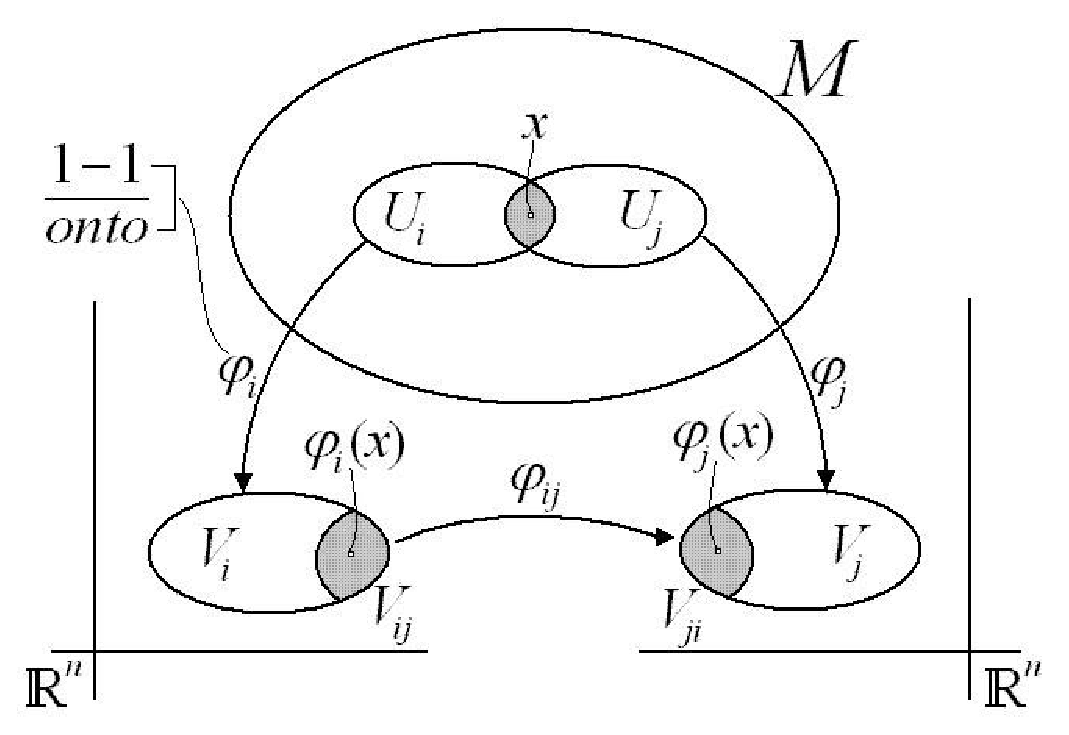
\includegraphics[width=9cm]{Manifold1}}
\caption{流形概念的几何图。}
\label{Manifold1}
\end{figure}

显然,任意一个点 $x\in M$ 可以有几个不同的图表(参见图 \ref{Manifold1})。考虑两个图表的情况, $\varphi _{i},\varphi
_{j}:M\rightarrow \mathbb{R}^{n}$,在它们的象中具有两个开集, $V_{ij}=\varphi _{i}(U_{i}\cap U_{j})$ 和 $V_{ji}=\varphi _{j}(U_{i}\cap
U_{j})$。那么我们在它们之间有转移函数(\textit{transition functions}) $\varphi _{ij}$,
\begin{equation*}
\varphi _{ij}=\varphi _{j}\circ \varphi _{i}^{-1}:V_{ij}\rightarrow
V_{ji},\qquad \text{locally given by\qquad }\varphi _{ij}(x)=\varphi
_{j}(\varphi _{i}^{-1}(x)).
\end{equation*}
如果转移函数 $\varphi _{ij}$ 存在,那么我们说,这两个图表,$\varphi _{i}$ 和 $\varphi _{j}$ 是兼容的(\emph{compatible})。转移函数表示一般(非线性)的坐标变换(\emph{transformations of coordinates}),这是经典张量微积分(\emph{tensor calculus})的核心。

一个兼容的图表 $\varphi _{i}:M\rightarrow \mathbb{R}^{n}$ 的集合,它使得每个点 $x\in M$ 在至少一个图表中有其欧几里得象,被称为一个图集(\textit{atlas})。两个图集是等价的(\emph{equivalent}),当且仅当它们的所有图表都是兼容的(即,它们之间存在转移函数),所以它们的并集同样也是一个图集。一个流形结构(\textit{manifold structure})是一类等价图集。

最后,由于图表 $\varphi _{i}:M\rightarrow \mathbb{R}^{n}$ 被认为是1--1并且是盖射映射,它们可以是同胚的(\emph{homeomorphism}\emph{s}),在这种情况下,我们有一个拓扑的(\emph{topological}) ($C^{0}$)流形,或者是微分同胚的(\emph{diffeomorphism}\emph{s}),在这种情况下,我们有一个光滑的(\emph{smooth}) ($C^{k}$)流形。

\subsection{光滑流形的形式定义}

给定一个图表 $( U,\varphi ) $,我们将集合U称为一个坐标域(\textit{coordinate domain}),或是其每个点的坐标邻域(coordinate neighborhood)。此外,如果在 $\mathbb{R}^{n}$ 中,$\varphi (U)$ 是一个开球,则 $U$ 被称为坐标球(\textit{coordinate ball})。映射 $\varphi $ 被称为局部的(\emph{local})坐标映射(\textit{coordinate map}),并且由 $\varphi (m)=( x^{1}(m),...,x^{n}(m)) $ 定义的 $\varphi $ 的分量函数 $( x^{1},...,x^{n}) $ 被称为 $U$ 上的局部坐标(\emph{local coordinates}) \cite{GaneshSprBig,GaneshADG}。

两个图表 $( U_{1},\varphi _{1}) $ 和 $( U_{2},\varphi _{2}) $ ,如果 $\varphi _{1}(U_{1}\cap U_{2})$ 和 $\varphi _{2}(U_{2}\cap U_{1})$ 是 $\mathbb{R}^{n}$ 的开子集,则使得 $U_{1}\cap U_{2}\neq \varnothing $ 被称为是兼容的(\emph{compatible})。一个在 $M$ 上的兼容图表 $( U_{\alpha },\varphi _{\alpha }) _{\alpha\in A}$ 族,使得 $U_{\alpha }$ 形成 $M$ 的覆盖(\emph{covering}),被称为一个图集(\emph{atlas})。对于图集$( U_{\alpha },\varphi _{\alpha }) _{\alpha \in A}$ 来说,其中 $U_{\alpha \beta }=U_{\alpha }\cap U_{\beta }$,映射 $\varphi _{\alpha \beta}=\varphi _{\beta }\circ \varphi _{\alpha }^{-1}:\varphi _{\alpha }(U_{\alpha \beta }) \rightarrow \varphi _{\beta }( U_{\alpha \beta }) $ 被称为转移映射(\emph{transition maps}),因此我们有一个可交换三角形:
\begin{equation*}
\Atriangle<1`1`1;500>[U_{\alpha \beta }\subseteq M`\varphi _{\alpha }(
U_{\alpha \beta }) `\varphi _{\beta }( U_{\alpha \beta }) ;\varphi _{\alpha
}`\varphi _{\beta }`\varphi _{\alpha \beta }]
\end{equation*}

对于流形 $M$ 的一个图集 $( U_{\alpha },\varphi _{\alpha }) _{\alpha \in A}$ 被称为 $C^{k}$ 图集($C^{k}-$\emph{atlas}),如果其所有转移映射 $\varphi
_{\alpha \beta }:\varphi _{\alpha }( U_{\alpha \beta }) \rightarrow \varphi
_{\beta }( U_{\alpha \beta }) $ 都是 $C^{k}$ 类型时。对于 $M$ ,两个 $C^{k}$ 图集被称为 $C^{k}$ 等价($C^{k}-$\emph{equivalent}),如果它们的并集再次是一个 $C^{k}$ 的图集时。一个 $C^{k}$ 图集的等价类被称为 $M$ 上的 $C^{k}$ 结构($C^{k}-$\emph{structure})。换句话说,一个 $M$ 上的光滑结构是 $M$ 上的一个最大的(\emph{maximal})光滑图集,即这样一个图集不包含在任何严格意义上更大的光滑图集中。我们所说的一个 $C^{k}$ 流形($C^{k}-$\emph{manifold}) $M$ ,是指一个带有 $C^{k}$ 结构的拓扑流形,并且 $M$ 上的图表将是属于 $C^{k}$ 结构的某个图集的图表。平滑流形是指 $C^{\infty }$流形($C^{\infty }-$manifold),``光滑(\emph{smooth})''一词与 $C^{\infty }$ 同义。

有时使用术语``局部坐标系统(local coordinate system)''或``参数化(parametrization)''来代替图表。 $M$ 不是用任何特定的图集来定义的,而是用图集的等价类来定义的,这是广义协变(\emph{general covariance})原理的一个数学表述。每一个合适的坐标系统都是同样的好。对于 $\mathbb{R}^{n}$ 的一个开放子集来说,一个欧几里得图表可能就足够了,但该坐标系统并不优于其它坐标系统,后者可能需要许多图表(如使用极坐标),但在其它方面更方便。

例如,一个$n$维球面的图集 $S^{n}$ 有两个图表。如果 $N=(1,0,...,0)$ 和 $S=(-1,...,0,0)$ 分别是 $S^{n}$ 的北极和南极,则这两个图表由 $N$ 和 $S$ 的立体投影给出为:
\begin{eqnarray*}
\varphi _{1} &:&S^{n}\backslash \{N\}\rightarrow \mathbb{R}^{n},\varphi
_{1}(x^{1},...,x^{n+1})=(x^{2}/(1-x^{1}),\ldots ,x^{n+1}/(1-x^{1})),\;\,
\text{and} \\
\varphi _{2} &:&S^{n}\backslash \{S\}\rightarrow \mathbb{R}^{n},\varphi
_{2}(x^{1},...,x^{n+1})=(x^{2}/(1+x^{1}),\ldots ,x^{n+1}/(1+x^{1})),
\end{eqnarray*}
而重叠映射 $\varphi _{2}\circ \varphi _{1}^{-1}:\mathbb{R}^{n}\backslash \{0\}\rightarrow \mathbb{R}^{n}\backslash \{0\}$ 由微分同胚 $(\varphi _{2}\circ \varphi _{1}^{-1})(z)=z/||z||^{2}$ 给出,对于 $\mathbb{R}^{n}\backslash \{0\}$ 中的 $z$,从 $\mathbb{R}^{n}\backslash \{0\}$ 映射到其自身。

可以在 $\mathbb{R}^{n}$ 上施加各种附加结构(\emph{additional structures}),相应的流形 $M$ 将通过其图表覆盖来继承这些结构。例如,如果图表覆盖在巴拿赫空间(\textit{Banach space}) $E$ 中取值,则 $E$ 被称为模型空间(\textit{model space}),并且  $M$ 被称为以 $E$ 为模型的 $C^{k}$ 巴拿赫流形($C^{k}-$\textit{Banach manifold})。同样地,如果图表覆盖在希尔伯特空间(\textit{Hilbert space}) $\mathcal{H}$ 中取值,则 $\mathcal{H}$ 被称为模型空间(\textit{model space}),并且  $M$ 被称为以 $\mathcal{H}$ 为模型的 $C^{k}$ 希尔伯特流形($C^{k}-$\textit{Hilbert manifold})。如果没有另外指定,我们将认为 $M$ 是欧几里得流形,其图表覆盖在 $\mathbb{R}^{n}$ 中获取它们的值。

对于 Hausdorff $C^{k}$ 流形来说,以下性质是等价的:(i) 它是仿紧的;(ii) 它是可度量的;(iii) 它允许黎曼度量;\footnote{%
回想欧几里得度量(\textit{Euclidean metric}) $d$ 的相应性质。对于任意三个点 $x,y,z\in \mathbb{R}^{n}$,以下公理是有效的:
\begin{eqnarray*}
M_{1} &:&d(x,y)>0,\text{ \ for \ }x\neq y;\qquad\text{and}\qquad d(x,y)=0,%
\text{ \ for \ }x=y; \\
M_{2} &:&d(x,y)=d(y,x); \qquad\qquad\quad M_{3}~: d(x,y)\leq d(x,z)+d(z,y).
\end{eqnarray*}%
} (iv) 每个连通部件是可分离的。

\subsection{光滑流形之间的光滑映射}

在两个流形 $M$ 和 $N$ 之间的映射 $\varphi :M\rightarrow N$ ,其中 $M\ni m\mapsto \varphi (m)\in N$,被称为光滑映射(\emph{smooth map}),或 $C^{k}$ 映射,如果我们有以下图表 \cite{GaneshSprBig,GaneshADG}:\newline
\bigbreak

\begin{equation*}
\bfig \putsquare<1`1`1`1;2000`1000>(0,0)[\odot`\odot`\odot`\odot;
\varphi`\phi`\psi`\psi \circ \varphi \circ \phi ^{-1}]
\put(50,1050){\oval(1000,600)}\put(1900,1050){\oval(1000,600)}
\put(-100,1050){\oval(450,400)}\put(2050,1050){\oval(450,400)}
\put(-150,1100){$U$}\put(-130,930){$m$} \put(2000,1100){$V$}\put(2020,930){$%
\varphi(m)$} \put(400,1100){$M$}\put(1450,1100){$N$}
\put(-20,-30){\oval(500,530)}\put(2000,-30){\oval(500,530)} \put(-220,100){$%
\phi(U)$}\put(2050,100){$\psi(V)$} \put(-120,-150){$\phi(m)$}\put(1830,-150){%
$\psi(\varphi(m))$} \putsquare<0`-1`0`1;1000`900>(-450,-450)[``\mathbb{R}%
^m`;```] \putsquare<0`0`-1`-1;1000`900>(1400,-450)[```\mathbb{R}^n;```] \efig
\end{equation*}

\noindent 这意味着对于每个 $m\in M$ 和 $N$ 上的每个图表,其中 $\varphi \left( m\right) \in V$ ,这是一个在 $M$ 上的图表 $\left( U,\phi \right) $,其中 $m\in U,\varphi \left( U\right)
\subseteq V$,并且 $\Phi =\psi \circ \varphi \circ \phi ^{-1}$ 是 $C^{k}$,也就是说,下面的图可交换:
\begin{equation*}
\square <1`1`1`1;1000`500>[M\supseteq U`V\subseteq N`\phi (U)`\psi
(V);\varphi `\phi `\psi `\Phi ]
\end{equation*}

设 $M$ 和 $N$ 是光滑流形,并且设 $\varphi :M\rightarrow N$ 是一个光滑映射。映射 $\varphi $ 被称为覆盖(\emph{covering}),或者等价地,$M$ 被称为覆盖(\emph{cover}) $N$,如果 $\varphi $ 是满射的,并且每个点 $n\in N$ 都有一个开放邻域 $V$ ,使得 $\varphi ^{-1}(V)$ 是一个不相交开集的并集,每个微分同胚都通过 $\varphi $ 映射到 $V$。

一个 $C^{k}$ 映射 $\varphi :M\rightarrow N$ 被称为 $C^{k}$ 微分同胚($C^{k}-$\textit{diffeomorphism}),如果 $\varphi $ 是一个双射,$\varphi ^{-1}:N\rightarrow M$ 存在并且也是 $C^{k}$。两个流形被称为是微分同胚的(diffeomorphic),如果两个流形之间存在一个微分同胚。所有的光滑流形和它们之间的光滑映射构成了范畴 $\mathcal{M}$。

\subsection{正切丛与拉格朗日动力学}

一个光滑 $n$ 维流形的正切丛(tangent bundle)是切向量所在的地方,并且它本身是一个光滑的 $2n$ 流形。向量–场是正切丛的横截面。拉格朗日量(\textit{Lagrangian})是正切丛上的自然能量函数(参见文献 \cite{GaneshSprBig,GaneshADG})。

在力学中,对于每个 $n$D 构型流形(\textit{configuration manifold}) $M$ 都有其 $2n$D 速度相空间流形(\textit{velocity phase--space manifold}),用 $TM$ 表示,并且其被称为 $M$ 的正切丛(参见图 \ref{TBun1})。原始的光滑流形 $M$ 被称为 $TM$ 的基(\emph{base})。这里有一个盖射映射 $\pi:TM\rightarrow M$,被称为投影(\emph{projection})。在每一个点 $x\in M$ 上方有一个在 $x$ 处与 $M$ 相切的切空间(\textit{tangent space}) $T_x M=\pi^{-1}(x)$ ,其被称为纤维丛(\textit{fibre})。纤维丛 $T_x M\subset TM$ 是 $TM$ 的子集,使得总的正切丛, $TM=\dbigsqcup\limits_{m\in M}T_x M$ ,是所有的点 $x\in M$ 的切空间 $T_x M$ 到 $M$ 的不相交并集(\emph{disjoint union})。从动力学角度来看,正切丛概念中最重要的量是光滑映射 $v:M\rightarrow TM$,它是投影 $\pi$ 的逆映射,即 $\pi\circ v=\func{Id}_M,\;\pi(v(x))=x$。它被称为速度向量–场(\textit{velocity vector--field})。它的图形 $(x,v(x))$ 表示正切丛 $TM$ 的横截面(\textit{cross--section})。这解释了动力学术语速度相空间(\textit{velocity phase--space}),为所给定的流形 $M$ 的正切丛 $TM$ 。
\begin{figure}[h]
\centerline{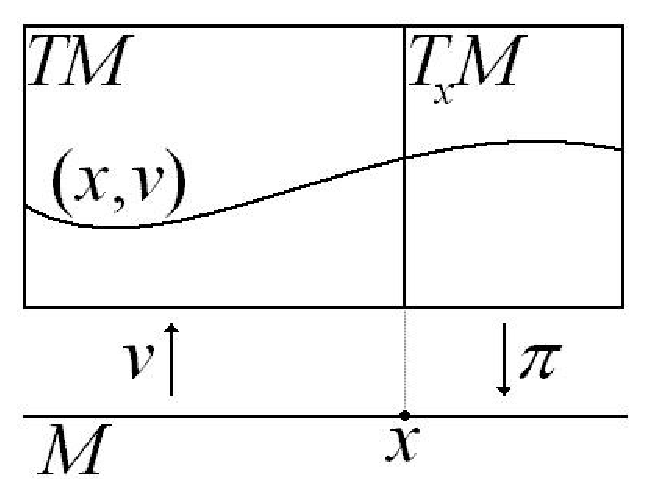
\includegraphics[width=4.5cm]{TanBundle1}}
\caption{光滑流形 $M$ 的正切丛 $TM$ 的速写。}
\label{TBun1}
\end{figure}

如果 $[a,b]$ 是封闭区间,则一个 $C^{0}$ 映射 $\gamma :[a,b]\rightarrow M$ 被称为在其端点 $a$ 处是可微的(\emph{differentiable}),如果在 $\gamma (a)$ 处有一个图表 $( U,\phi ) $ ,使得以下极限存在并且是有限的:
\begin{equation}
{\frac{d}{dt}}(\phi \circ \gamma )(a)\equiv(\phi \circ \gamma )^{\prime
}(a)=\lim_{t\rightarrow a}\frac{(\phi \circ \gamma )(t)-(\phi \circ \gamma
)(a)}{t-a}.  \label{limit}
\end{equation}
概化方程 (\ref{limit}),我们得到了流形上曲线(\emph{curve on a manifold})的概念。对于一个光滑流形 $M$ 和一个点 $m\in M$ ,在 $m$ 处的一条曲线为一个 $C^{0}$ 映射 $\gamma :I\rightarrow M$ ,它从区间 $I\subset \mathbb{R}$ 使用 $0\in I$ 和 $\gamma (0)=m$ 映射进入 $M$。

通过一个点 $m\in U$的两条曲线 $\gamma _{1}$ 和 $\gamma _{2}$ ,相对于图表 $( U,\phi ) $,相切于(\emph{tangent at})点 $m$ 处,如果 $(\phi \circ \gamma _{1})^{\prime }(0)=(\phi \circ \gamma _{2})^{\prime }(0)$。因此,如果两条曲线在流形上的局部图表中具有完全相同的切向量(相同的方向和速度),则它们是相切的。

对于一个光滑流形 $M$ 和一个点 $m\in M$ ,在 $m$ 处到 $M$ 的切空间(\emph{tangent space}) $T_{m}M$ 是在 $m$ 处的曲线的等价类集合(\emph{set of equivalence classes}):
\begin{equation*}
T_{m}M=\{ [ \gamma ] _{m}:\gamma \text{ is a curve at a point }m\in M\} .
\end{equation*}

两个流形 $M$ 和 $N$ 之间的一个 $C^{k}$ 映射 $\varphi :M\ni m\mapsto \varphi (m)\in N$ 对于每一点 $m\in M$ 诱导出一个线性映射 $T_{m}\varphi :T_{m}M\rightarrow T_{\varphi (m)}N$ ,则被称为切映射(\textit{tangent map}),如果我们有:\newline
$\quad$\newline

\begin{equation*}
\bfig \putsquare<1`1`1`1;2000`1000>(0,0)[\,\odot`\,\,\odot`\,\odot`\,\,%
\odot; T(\varphi)`\pi_M`\pi_N`\varphi]
\put(-500,750){\framebox(1000,600){}}\put(1500,750){\framebox(1030,600){}}
\put(0,0){\oval(1000,400)}\put(2000,0){\oval(1000,400)} \put(-100,-100){$m$%
}\put(2050,-100){$\varphi(m)$} \put(-400,0){$M$}\put(2300,0){$N$}
\multiput(-500,750)(100,0){10}{\line(0,1){600}}
\multiput(1500,750)(100,0){10}{\line(0,1){600}} \put(270,1400){$TM$%
}\put(1500,1400){$T(N)$} \put(-150,1400){$T_m(M)$}\put(1850,1400){$%
T_{\varphi(m)}(N)$} \linethickness{0.3mm}\put(0,750){\line(0,1){600}}
\put(2000,750){\line(0,1){600}} \efig
\end{equation*}
\bigbreak\bigbreak \noindent 即下图可交换:
\begin{equation*}
\square <1`1`1`1;1000`500>[T_{m}M`T_{\varphi (m)}N`M\ni m`\varphi (m)\in
N;T_{m}\varphi `\pi _{M}`\pi _{N}`\varphi ]
\end{equation*}
其中自然投影(\textit{natural projection}) $\pi _{M}:TM\rightarrow M$ ,由 $\pi_{M}( T_{m}M) =m$ 给出,它给点 $m\in M$ 带来一个切向量 $v$ ,并且向量 $v$ 附着在该点,即 $v\in T_{m}M$。

对于一个 $n$D 光滑流形M,其 $M$ 正切丛(\textit{tangent bundle}) $TM$ 是其在所有的点 $m\in M$ 处的所有切空间 $T_{m}M$ 的不相交并集,$TM=\dbigsqcup\limits_{m\in M}T_{m}M$。

为了定义 $TM$ 上的光滑结构,我们需要指定如何在 $TM$ 上构造局部坐标。为此,设 $( x^{1}(m),...,x^{n}(m)) $ 为 $M$ 上的一个点 $m$ 的局部坐标,设 $( v^{1}(m),...,v^{n}(m)) $ 为该坐标系统中切向量的分量。则 $2n$ 个数 $( x^{1}(m),...,x^{n}(m),\,v^{1}(m),...,v^{n}(m)) $ 给出 $TM$ 上的局部坐标系统(\emph{local coordinate system})。

$TM=\dbigsqcup\limits_{m\in M}T_{m}M$ 定义了一个由 $M$ 参数化的向量空间族。在自然投影 $\pi _{M}$ 下,一个点 $m\in M $ 的逆映射象 $\pi _{M}^{-1}(m)$ 是切空间 $T_{m}M$。该空间被称为在点 $m\in M $ 上的正切丛的纤维丛(\emph{fibre})。

两个流形 $M$ 和 $N$之间的 $C^{k}$ 映射 $\varphi :M\rightarrow N$ 在它们的正切丛之间诱导出一个线性切映射(\textit{tangent map}) $T\varphi:TM\rightarrow TN$ ,也就是说,以下的图是可交换的:
\begin{equation*}
\square <1`1`1`1;900`500>[TM`TN`M`N;T\varphi`\pi _{M}`\pi _{N}`\varphi ]
\end{equation*}

所有的正切丛和它们的切映射构成了范畴 $\mathcal{TB}$。范畴 $\mathcal{TB}$ 是拉格朗日动力学(\textit{Lagrangian dynamics})的自然框架。

现在,我们可以制定链式规则的全局版本(\emph{global version of the} \emph{chain rule})。如果 $\varphi :M\rightarrow N$ 和 $\psi :N\rightarrow P$ 是两个光滑映射,则我们有 $T(\psi \circ \varphi )=T\psi \circ T\varphi $。换句话说,我们有一个从光滑流形的范畴 $\mathcal{M}$ 到其正切丛的范畴 $\mathcal{TB}$ 的函子(functor) $T:\mathcal{M\Rightarrow TB}$ :
\begin{equation*}
\Atriangle<1`1`1;500>[M`N`P;\varphi `(\psi \circ \varphi )\qquad \overset{T}{%
\Longrightarrow }`\psi ]\qquad \Atriangle<1`1`1;500>[TM`TN`TP;T\varphi
`T(\psi \circ \varphi )`T\psi ]
\end{equation*}

\subsection{余切丛与哈密顿动力学}

一个光滑 $n$ 维流形的余切丛位于1–形式(1--forms)存在的地方,并且它本身是一个光滑的 $2n$ 维流形。协向量–场(Covector--fields, 1--forms)是余切丛的横截面。哈密顿量(\textit{Hamiltonian})是余切丛上的自然能量函数(参见文献 \cite{GaneshSprBig,GaneshADG})。

对于光滑流形 $M$ 在点 $m$ 处的切空间 $T_{m}M$ 的对偶(\emph{dual})概念是其在同一点 $m$ 处的余切空间(\textit{cotangent space}) $T_{m}^{\ast }M$。与正切丛相似,对于维数为 $n$ 的光滑流形 $M$,它的余切丛(\textit{cotangent bundle}) $T^{\ast }M$ 是其在所有的点 $m\in M$ 处的所有余切空间 $T_{m}^{\ast }M$ 的不相交并集,即 $T^{\ast }M=\dbigsqcup\limits_{m\in M}T_{m}^{\ast }M$。因此,$n$ 维流形 $M$ 的余切丛是向量丛 $T^{\ast}M=(TM)^{\ast }$,正切丛 $TM$ 的(实)对偶。

如果 $M$ 是一个 $n$ 维流形,则 $T^{\ast }M$ 是一个 $2n$ 维流形。为了定义 $T^{\ast }M$ 上的光滑结构,我们需要指定如何在 $T^{\ast }M$ 上构造局部坐标。为此,设 $( x^{1}(m),...,x^{n}(m))$ 为 $M$ 上一个点 $m$ 的局部坐标,并设 $(p_{1}(m),...,p_{n}(m)) $ 为该坐标系统中一个协向量(covector)的分量。则 $2n$ 个数 $(x^{1}(m),...,x^{n}(m),\,p_{1}(m),...,p_{n}(m)) $ 给出一个 $T^{\ast }M$ 上的局部坐标系统。这就是人们用来证明 $T^{\ast }M$ 确实是一个 $2n$ 维流形的基本思路。

$T^{\ast }M=\dbigsqcup\limits_{m\in M}T_{m}^{\ast }M$ 定义了一个由 $M$ 参数化的向量空间族,其中协自然投影(\textit{conatural projection}),$\pi _{M}^{\ast }:T^{\ast }M\rightarrow M$,由 $\pi _{M}^{\ast }(T_{m}^{\ast }M) =m$ 给出,它给点 $m\in M$ 带来一个余切向量 $p$,并且余切向量 $p$ 附着在该点,即 $p\in T_{m}^{\ast }M$。点 $m\in M$ 的逆映射象 $\pi _{M}^{-1}(m)$ 在协自然投影 $\pi _{M}^{\ast }$ 下是余切空间 $T_{m}^{\ast }M$。该空间被称为点 $m\in M$ 上的余切丛的纤维丛(\emph{fibre})。

以类似的方式,两个流形 $M$ 和 $N$ 之间的 $C^{k}$ 映射 $\varphi :M\rightarrow N$ 在它们的余切丛之间诱导出一个线性余切映射(\emph{cotangent map}) $T^{\ast}\varphi :T^{\ast }M\rightarrow T^{\ast }N$ ,也就是说,以下的图是可交换的:
\begin{equation*}
\square <1`1`1`1;900`500>[T^{\ast }M`T^{\ast }N`M`N;T^{\ast }\varphi `\pi
_{M}^{\ast }`\pi _{N}^{\ast }`\varphi ]
\end{equation*}

所有余切丛和它们的余切映射构成了范畴 $\mathcal{T^{\ast }B}$。范畴 $\mathcal{T^{\ast }B}$ 是哈密顿动力学(\textit{Hamiltonian dynamics})的自然阶段。

现在,我们可以制定全局链式规则的对偶版本(\emph{dual version of the global chain rule})。如果 $\varphi :M\rightarrow N$ 和 $\psi :N\rightarrow P$ 是两个光滑映射,则我们有 $T^{\ast }(\psi \circ \varphi )=T^{\ast }\psi \circ T^{\ast}\varphi $。换句话说,我们有一个从光滑流形的范畴 $\mathcal{M}$ 到它们的余切丛的范畴 $\mathcal{T^{\ast }B}$ 的协函子(cofunctor) $T^{\ast }:\mathcal{M\Rightarrow T^{\ast }B}$:
\begin{equation*}
\Atriangle<1`1`1;500>[M`N`P;\varphi `(\psi \circ \varphi )\qquad \overset{%
T^{\ast }}{\Longrightarrow }`\psi ]\qquad \Atriangle<-1`-1`-1;500>[T^{\ast
}M`T^{\ast }N`T^{\ast }P;T^{\ast }\varphi `T^{\ast }(\psi \circ \varphi
)`T^{\ast }\psi ]
\end{equation*}

\section{李群}

在本节中,我们介绍李群的经典理论(\textit{classical theory of Lie groups})基础及其李代数,它们主要由Sophus Lie、Elie Cartan、Felix Klein、Wilhelm Killing和Hermann Weyl开发。关于更多的综合资料,参见文献 \cite{Chevalley,Helgason,Gilmore,Fulton,Bourbaki}。

19世纪中叶,S.Lie 有一个影响深远的发现,即设计用于求解特定不相关类型的常微分方程(ODE)的技术,例如可分离的、齐次的和精确的方程,实际上都是基于微分方程在连续对称群下的不变性的一般形式群积分程序的特例。粗略地说,微分方程组的对称群是将一个系统的解转换为其它解的群。一旦确定了对称群,就可以使用一些技术来求解和分类这些微分方程。在 Lie 的经典框架中,这些群是局部群,并做为一些欧几里得空间上的变换群而产生于局部。从局部的李群到今天使用流形的定义是由E.Cartan在19世纪末完成的,他的工作是李理论、经典几何、微分几何和拓扑学的一个引人注目的综合。

这些连续群,最初做为微分方程的对称群出现,多年来对代数拓扑、微分几何、数值分析、控制理论、经典力学、量子力学等不同领域产生了深远影响。它们现在被普遍称为李群。

李群是光滑流形,它也具有一个群结构,其乘积和逆运算做为流形的映射是光滑的。这些对象在描述物理对称性时自然产生。\footnote{%
下面是一些李群的例子,以及它们与数学和物理学领域的关系:
\par
\begin{enumerate}
\item 欧几里得空间 $\mathbb{R}^{n}$ 是阿贝尔李群(以普通向量加法做为群运算)。
\par
\item 可逆矩阵(在矩阵乘法下)的群 $GL_{n}(\mathbb{R})$ 是维数为 $n^{2}$ 的李群。它有一个行列式为 1 的矩阵的子群 $SL_{n}(\mathbb{R})$,也是李群。
\par
\item 由 $n$D 向量空间的所有旋转和反射产生的群 $O_{n}(\mathbb{R})$ 是一个被称为正交群(\textit{orthogonal group})的李群。它有一个行列式为 1 的元素子群,被称为特殊正交群 $SO(n)$,它是 $\mathbb{R}^{n}$中的旋转群(\textit{group of rotations})。
\par
\item 自旋群是特殊正交群的双重覆盖(例如被用于研究量子场论中的费米子)。
\par
\item 所有保留对称形式的矩阵的群 $Sp_{2n}(\mathbb{R})$ 是一个李群,被称为对称群(\textit{symplectic group})。
\par
\item 时空等距的洛伦兹群和庞加莱群是维数为 6 和 10 的李群,在狭义相对论中使用。
\par
\item 海森堡群是一个维数为3的李群,在量子力学中使用。
\par
\item 酉群 $U(n)$ 是由酉矩阵组成的维数为 $n^{2}$ 的紧群。它有一个行列式为 1 的元素子群,被称为特殊酉群 $SU(n)$。
\par
\item 群 $U(1)\times SU(2)\times SU(3)$ 是一个维数为 $1+3+8=12$ 的李群,它是基本粒子标准模型的规整群,其维数对应于:1个光子 + 3个向量玻色子 + 8个胶子。
\end{enumerate}
}

李群是一个群,其元素可以用实数连续参数化,例如旋转群(\textit{rotation group}) $SO(3)$,它可以用欧拉角(\textit{Euler angles})参数化。更正式地说,李群是一个解析实流形或复流形,也是一个群,因此群运算乘法和逆是解析映射。李群在数学分析、物理学和几何学中很重要,因为它们有助于描述分析结构的对称性。它们由 \emph{Sophus} \textit{Lie} 于1870年提出,目的是研究微分方程的对称性。

虽然欧几里得空间 $\mathbb{R}^{n}$ 是一个实李群(\textit{real Lie group}) (以普通向量加法做为群运算),但是更典型的例子由矩阵李群给出,即可逆矩阵群(在矩阵乘法下)。例如,在 $\mathbb{R}^{3}$ 中所有旋转的群 $SO(3)$ 是一个矩阵李群。

人们根据李群的代数性质(\textit{algebraic properties})%
\footnote{%
如果 $G$ 和 $H$ 是李群(均为实李群或均为复李群),则一个李群同态(\textit{Lie--group--homomorphism}) $f:G\rightarrow H$ 是一个群同态(\textit{group homomorphism}),也是一个解析映射(\textit{analytic map}) (人们可以证明这是等价的,仅要求该 $f$ 是连续的)。两个这样的同态的组合再次是同态,并且所有(实数的或复数的)李群的种类与这些态射一起形成一个范畴。两个李群被称为同构(\textit{isomorphic}),当且仅当它们之间存在一个双射同态,其逆也是同态。同构李群不需要以所有实际意图做区分;它们仅在元素的符号上有所不同。} (简单的、半单的、可解的、幂零的、阿贝尔的)、它们的连通性(\textit{connectedness}) (连通的或单连通的) 和它们的紧性(\textit{compactness})来分类李群。\footnote{%
一个 $n$ 维环面 $T^n=S^1 \times S^1\times\cdots\times S^1$ (如上定义)是紧致阿贝尔李群(\textit{compact Abelian Lie group})的一个例子。这是因为单位圆 $S^1$ 是一个紧致阿贝尔李群(当用乘法的单位复数识别时)。然后,$T^n$ 上的群乘法由坐标乘法定义。
\par
环面群在紧致李群理论中起着重要作用。这在一定程度上是因为在任意紧致李群中,人们总能找到一个最大环面;即一个封闭子群,它是一个最大可能维数的环面。}

对于每个李群,我们可以关联一个李代数(\textit{Lie algebra}),该李代数完全捕获了群的局部结构(至少如果李群是连通的时候)。\footnote{%
传统上,人们可以将李群上切向量的任意场 $X$ 视为偏微分算子,用 $Xf$ 表示标量场 $f$ 在 $X$ 的方向上的李导数(\textit{Lie derivative})或方向导数(\textit{directional derivative})。然后,如果李群 $G$ 上的向量–场与左平移进行变换,则称其为左不变(left--invariant),这意味着如下性质。对于任意解析函数 $f:G\rightarrow \mathbb{R}$ 和所有的 $g,x\in G$,定义 $L_{g}[f](x)=f(gx)$。则向量–场 $X$ 是左不变的,当且仅当对于所有的 $g\in G$,$XL_{g}=L_{g}X$。类似地,我们可以使用 $\mathbb{C}$ 代替 $\mathbb{R}$。在解析流形上所有向量–场的集合是 $\mathbb{R}$ (或$\mathbb{C}$)上的李代数(\textit{Lie algebra})。
\par
在李群G上,左不变向量–场形成一个子代数,即与 $G$ 相关的李代数 $\mathfrak{g}$。这个李代数是有限维的(它与流形 $G$ 具有相同的维数),这使得它容易受到分类尝试的影响。通过对 $\mathfrak{g}$ 进行分类,人们也可以掌握该群 $G$。简单李群的表示理论是最好的和最重要的例子。
\par
在 $G$ 的单位元素 $e$ 处的切空间 $T_{e}$ 的每个元素 $v$ 确定唯一的左不变向量–场,其在 $G$ 的元素 $g$ 处的值由 $gv$ 表示;李代数 $\mathfrak{g}$ 下面的向量空间因此可以被标识为 $T_{e}$。
\par
李代数 $\mathfrak{g}$ 中的每个向量–场 $v$ 确定一个函数 $c:\mathbb{R}\rightarrow G$,其导数处处由相应的左不变向量–场: $c^{\prime}(t)=TL_{c(t)}v$ 给出,并且具有性质:$c(s+t)=c(s)c(t),\qquad (\text{对于所有的 $s$ 和 $t$})$ (在右手侧的运算是在 $G$ 中的群乘法)。对于初等指数函数,该公式用一种有效的形式相似性证明了定义:$\mathrm{exp}(v)=c(1)$。这被称为指数映射(\textit{exponential map}),并且它将李代数 $\mathfrak{g}$ 映射到李群 $G$ 中。它提供了 $\mathfrak{g}$\ 中 $0$ 的邻域和 $G$ 中 $e$ 的邻域之间的微分同胚(\textit{diffeomorphism})。该指数映射是指数函数对于实数(因为 $\mathbb{R}$ 是具有乘法的正实数的李群的李代数),对于复数(因为 $\mathbb{C}$ 是具有乘法的非零复数的李群的李代数)和对于矩阵(因为具有正则交换子的 $M(n,\mathbb{R})$ 是所有可逆矩阵的李群 $GL(n,\mathbb{R})$ 的李代数)的概化。由于指数映射在 $e$ 的某个邻域 $N$ 上是满射的,所以通常调用群 $G$ 的李代数无穷小生成元(\textit{infinitesimal generators})的元素。
\par
指数映射和李代数决定了每个连通李群的局部群结构,因为BCH公式(\textit{Baker--Campbell--Hausdorff formula}):李代数 $\mathfrak{g}$ 的零元素存在一个邻域 $U$,使得对于 $u,v\in U$,我们有
\begin{equation*}
\mathrm{exp}(u)\mathrm{exp}(v)=\mathrm{exp}%
(u+v+1/2[u,v]+1/12[[u,v],v]-1/12[[u,v],u]-...),
\end{equation*}
其中省略的项是已知的并且涉及四个或更多元素的李括号(\textit{Lie bracket}\emph{s})。在 $u$ 和 $v$ 可交换的情况下,该公式简化为熟悉的指数定律(\textit{exponential law}):
\begin{equation*}
\mathrm{exp}(u)\mathrm{exp}(v)=\mathrm{exp}(u+v).
\end{equation*}%
\par
李群的每个同态 $f:G\rightarrow H$ 在相应的李代数 $\mathfrak{g}$ 和 $\mathfrak{h}$ 之间引入一个同态。该关联 $G\Longrightarrow \mathfrak{g}$ 被称为李函子(\textit{Lie Functor})。}

\subsection{李群的定义}

李群(\textit{Lie group})是一个光滑的(Banach)流形 $M$,它同时具有与其流形 $M$ 结构一致的一个群 $G$ 结构,就其意义而言即群乘法(\textit{group multiplication}) $\mu :G\times G\rightarrow G,~~(g,h)\mapsto gh$,并且其群逆(\textit{group inversion}) $\nu :G\rightarrow G,~~g\mapsto g^{-1}$ 为 $C^{k}$ 映射。一个点 $e\in G$ 被称为群特征元素(\textit{group identity element}) (参见文献 \cite{Chevalley,Helgason,Arnold,Abraham})。

例如,任意 $n$D Banach 向量空间 $V$ 是一个阿贝尔李群,其具有群运算 $\mu :V\times V\rightarrow V$, $\mu (x,y)=x+y$,并且 $\nu :V\rightarrow V$, $\nu (x)=-x$。特征只是零向量。我们称这样的李群为向量群(\emph{vector group})。

设 $G$ 和 $H$ 是两个李群。一个映射被称为李群的态射(\emph{morphism}),或其光滑同态(\textit{smooth homomorphism}),如果它们是做为抽象群的同态和做为流形的光滑映射。

类似地,一个群 $G$,它在同一时间是一个拓扑空间,则它被称为拓扑群(\textit{topological group}),如果两个映射 ($\mu ,\nu $) 都是连续的,即对其是 $C^{0}$ 映射。拓扑群的同态 $G\rightarrow H$ 被称为是连续的,如果它是一个连续映射。

一个拓扑群(以及一个光滑流形)不一定是Hausdorff性质的。一个拓扑群 $G$ 是Hausdorff性质的,当且仅当其特征是封闭的。做为一个推论,我们得到每一个李群都是一个Hausdorff性质的拓扑群。

对于一个李群 $G$ 中的每一个 $g$,两个映射, \
\begin{eqnarray*}
L_{g} &:&G\rightarrow G,\qquad h\mapsto gh, \\
R_{h} &:&G\rightarrow G,\qquad g\mapsto gh,
\end{eqnarray*}
被称为左的(\emph{left})和右的平移(\textit{right translation})映射。因为 $L_{g}\circ L_{h}=L_{gh}$,以及 $R_{g}\circ R_{h}=R_{gh}$,由此可见 $\left( L_{g}\right) ^{-1}=L_{g^{-1}}$ 以及 $\left( R_{g}\right)^{-1}=R_{g^{-1}}$,因此 $L_{g}$ 和 $R_{g}$ 都是微分同胚。此外,$L_{g}\circ R_{h}=R_{h}\circ L_{g}$,即左的和右的平移可交换。

在 $G$ 上的一个向量–场 $X$ 被称为左不变向量–场(\emph{left--invariant vector--field}),如果对于每一个 $g\in G$,$L_{g}^{\ast }X=X$,这就是,如果对于所有的 $h\in G$,$(T_{h}L_{g})X(h)=X(gh)$,即下图可交换:
\begin{equation*}
\square <1`-1`-1`1;900`500>[TG`TG`G`G;TL_{g}`X`X`L_{g}]
\end{equation*}

一个李群 $G$ 上的黎曼度量(\textit{Riemannian metric})被称为左不变的,如果所有左平移 $L_{g}$ 都被保留,即如果左平移的导数将每个向量传输到一个相同长度的向量。类似地,在 $G$ 上的一个向量场 $X$ 被称为左不变的,如果对于每一个 $g\in G$,$L_{g}^{\ast }X=X$。

\subsection{李代数}

一个代数(\emph{algebra}) $A$ 是一个具有乘积的向量空间。该乘积必须具有以下性质
\begin{equation*}
a(uv)=(au)v=u(av),
\end{equation*}%
对于每一个 $a\in \mathbb{R}$ 和 $u,v\in A$。一个代数之间的映射 $\phi :A\rightarrow A^{\prime }$ 被称为代数同构(\textit{algebra homomorphism}),如果 $\phi (u\cdot v)=\phi (u)\cdot \phi (v)$。一个代数 $A$ 的一个向量子空间 $\mathfrak{I}$ 被称为左理想(\textit{left ideal}) (区别于右理想(\emph{right ideal})),如果它在代数乘法下是封闭的,并且如果 $u\in A$ 和 $i\in \mathfrak{I}$ 就意味着 $ui\in \mathfrak{I}$ (区别于 $iu\in \mathfrak{I}$%
)。一个子空间 $\mathfrak{I}$ 被称为双边理想(\emph{two--sided ideal}),如果它同时是左理想和右理想。一个理想可能不是一个代数本身,但是一个代数与一个双边理想的商(quotient)继承了来自 $A$ 的一个代数结构。

一个李代数(\emph{Lie algebra})是一个代数 $A$,其中的乘法,即李括号(\emph{Lie bracket}) $(u,v)\mapsto \lbrack u,v]$,具有以下性质:

LA 1. $[u,u]=0$ 对于每一个 $u\in A$,并且

LA 2. $[u,[v,w]]+[w,[u,v]]+[v,w,u]]=0$ 对于所有的 $u,v,w\in A$。

条件LA 2通常被称为雅可比恒等式(\textit{Jacobi identity})。一个李代数的子空间 $E\subset A$ 被称为李子代数(\textit{Lie subalgebra}),如果 $[u,v]\in E$ 对于每一个 $u,v\in E$。一个在李代数之间的映射 $\phi:A\rightarrow A^{\prime }$ 被称为李代数同态(\textit{Lie algebra homomorphism}),如果对于每一个 $u,v\in A$, $\phi
([u,v])=[\phi (u),\phi (v)]$。

所有李代数(在给定域 $\mathbb{K}$ 上)和它们之间的所有光滑同态形成范畴 $\mathcal{LAL}$,其本身是所有代数及其同态的范畴 $\mathcal{AL}$ 的完整子范畴。

设 $\mathcal{X}_{L}(G)$ 表示 $G$ 上的左不变向量–场集合;它是 $\mathcal{X}(G)$ 的一个李子代数,是 $G$ 上所有向量–场的集合,因为 $L_{g}^{\ast }[X,Y]=[L_{g}^{\ast }X,L_{g}^{\ast }Y]=[X,Y]$,所以李括号 $[X,Y]\in \mathcal{X}_{L}(G)$。

设 $e$ 是 $G$ 的特征元素。然后,对于切空间 $T_{e}G$ 上的每个 $\xi $,我们用 $X_{\xi}(g)=T_{e}L_{g}(\xi )$ 在 $G$ 上定义一个向量–场 $X_{\xi }$。$\mathcal{X}_{L}(G)$ 和 $T_{e}G$ 做为向量空间是同构的。对于所有的 $\xi ,\eta \in T_{e}G$,用 $\lbrack \xi ,\eta ]=\left[ X_{\xi },X_{\eta }\right] (e)$ 定义 $T_{e}G$ 上的李括号。这把 $T_{e}G$ 转变为李代数。此外,根据构造,我们有 $\left[X_{\xi },X_{\eta }\right] =X_{[\xi ,\eta ]}$;这在 $T_{e}G$ 中通过左延伸(\emph{left extension})定义了一个括号。具有上述代数结构的向量空间 $T_{e}G$ 被称为李群 $G$ 的李代数,并表示为 $\mathfrak{g}$。

例如,设 $V$ 是一个 $n$D 向量空间。则对于所有的 $\eta \in V$,$T_{e}V\simeq V$ 和由 $\xi \in T_{e}V$ 定义的左不变向量–场是恒定的向量–场 $X_{\xi }(\eta )=\xi $。$V$ 的李代数是 $V$ 本身。

由于阿贝尔李群 $G$ 的任意两个元素可交换,因此所有伴随算子 $Ad_{g}$,$g\in G$,等同于特征。因此,李代数 $g$ 是阿贝尔的;也就是说,对于所有的 $\xi ,\eta \in \mathfrak{g}$,$[\xi ,\eta ]=0$。

例如,$G=SO(3)$ 是3D欧几里得空间的旋转群,即固连在刚体上一个点的构型空间。机体的运动则由在 $SO(3)$ 群中的一条曲线 $g=g(t)$ 来描述。它的李代数 $\mathfrak{g}=\mathfrak{so}(3)$是所有可能的旋转的角速度的3D向量空间。该代数中的交换子是通常的向量(交叉)乘积(参见文献 \cite{Arnold,Abraham,GaneshADG})。

刚体(固连在一个点上)的旋转速度 $\dot{g}$ 是李群 $G=SO(3)$ 在该点 $g\in G$ 处的切向量。为了得到角速度,我们必须把这个向量带入群在特征处的切空间 $TG_{e}$,即带入它的李代数 $\mathfrak{g}=\mathfrak{so}(3)$。这可以通过两种方式实现:通过左平移 $L_{g}$ 和右平移 $R_{g}$。其结果是,我们在李代数中获得了两个不同的向量场 $\mathfrak{so}(3)$:

\begin{equation*}
\omega _{c}=L_{g^{-1}\ast }\dot{g}\in \mathfrak{so}(3)\qquad \text{and\qquad
}\omega _{x}=R_{g^{-1}\ast }\dot{g}\in \mathfrak{so}(3),
\end{equation*}%
它们分别被称为“机体中的角速度”和“空间中的角速度”。

对偶空间 $\mathfrak{g}^{\ast }$ 对于李代数 $\mathfrak{g}=\mathfrak{so}(3)$ 是角动量 $\mathbf{\pi }$ 的空间。机体的动能 $T$ 由机体中角速度的向量场决定,而不取决于机体在空间中的位置。因此,动能给出了在旋转群 $G=SO(3)$ 上的左不变黎曼度量。

\subsection{单参数子群}

设 $X_{\xi }$ 是 $G$ 上对应于 $\mathfrak{g}$ 中的 $\xi $ 的左不变向量–场,则存在 $X_{\xi }$ 的一条唯一的积分曲线 $\gamma _{\xi}:\mathbb{R}\rightarrow G$,起始于 $e$ 处,即(参见文献 \cite{GaneshSprBig,GaneshADG})
\begin{equation*}
\dot{\gamma}_{\xi }(t)=X_{\xi }\left( \gamma _{\xi }(t)\right) ,\qquad
\gamma _{\xi }(0)=e
\end{equation*}
$\gamma _{\xi }(t)$ 是 $G$ 的一个光滑单参数子群(\emph{one--parameter subgroup}),即$\gamma _{\xi }(t+s)=\gamma _{\xi }(t)\cdot \gamma _{\xi }(s)$,因为,做为 $t$ 的函数,两边在 $t=0$ 时都等于 $\gamma _{\xi }(s)$ ,并且通过 $X_{\xi }$ 的左不变性都满足微分方程 $\dot{\gamma}(t)=X_{\xi }\left( \gamma _{\xi}(t)\right) $,所以它们是相等的。左不变性也可以用来证明 $\gamma _{\xi }(t)$ 对所有的 $t\in \mathbb{R}$ 都是已定义的。此外,如果 $\phi :\mathbb{R}\rightarrow G$ 是 $G$ 的一个单参数子群,即加性群 $\mathbb{R}$ 进入 $G$ 的一个光滑同态(\emph{smooth homomorphism}),则 $\phi =\gamma _{\xi }$,其中 $\xi =\dot{\phi}(0)$,因为在关系式中于 $s=0$ 处取导数为
\begin{equation*}
\phi (t+s)=\phi (t)\cdot \phi (s)\qquad \text{gives\qquad }\dot{\phi}(t)=X_{%
\dot{\phi}(0)}\left( \phi (t)\right) ,
\end{equation*}%
所以 $\phi =\gamma _{\xi }$,因为在 $t=0$ 处两者都等于 $e$。因此,$G$ 的所有单参数子群对于某些 $\xi \in \mathfrak{g}$ 都是 $\gamma _{\xi }(t)$ 的形式。

\subsection{指数映射}

映射 $\exp :\mathfrak{g}\rightarrow G$,给出为 (参见文献 \cite{Abraham,GaneshSprBig,GaneshADG}):
\begin{equation*}
\exp (\xi )=\gamma _{\xi }(1),\qquad \exp (0) = e
\end{equation*}
其被称为 $G$ 的李代数 $\mathfrak{g}$ 进入 $G$ 的指数映射(\textit{exponential map})。$\exp $ 是一个 $C^{k}$ 映射,类似于正切丛和余切丛的投影 $\pi$;$\exp $ 是一个从在 $\mathfrak{g}$ 中的零邻域盖射到 $G$ 中的 $e$ 邻域的局部微分同胚;如果 $f:G\rightarrow H$ 是一个李群的光滑同态,则
\begin{equation*}
f\circ \exp _{G}=\exp _{H}\circ T_{e}f\,.
\end{equation*}

另外,在这种情况下
\begin{equation*}
\exp (s\xi )=\gamma _{\xi }(s).
\end{equation*}%
事实上,对于固连的 $s\in \mathbb{R}$,该曲线 $t\mapsto \gamma _{\xi }(ts)$,其在 $t=0$ 处通过 $e$,满足微分方程
\begin{equation*}
\frac{d}{dt}\gamma _{\xi }(ts)=sX_{\xi }\left( \gamma _{\xi }(ts)\right)
=X_{s\xi }\left( \gamma _{\xi }(ts)\right) .
\end{equation*}
由于 $\gamma _{s\xi }(t)$ 满足相同的微分方程,并在 $t=0$ 处通过 $e$,由此可见 $\gamma _{s\xi }(t)=\gamma _{\xi }(st)$。设置 $t=1$ 诱导出 $\exp (s\xi )=\gamma _{\xi }(s)$。

因此 $\exp $ 映射将 $\mathfrak{g}$ 中的直线 $s\xi$ 盖射到 $G$ 的单参数子群 $\gamma _{\xi }(s)$ 上,该子群在 $e$ 处与 $\xi$相切。从左不变性可知,$X$ 的流 $F_{t}^{\xi }$ 满足 $F_{t}^{\xi }(g)=g\exp (s\xi )$。

全局范围内,指数映射 $\exp$ 是一个自然操作,即,对于李群 $G$ 和 $H$ 的任意态射 $\varphi:G\rightarrow H$,以及一个李函子 $\mathcal{F}$,以下图可交换:
\begin{equation*}
\square <1`1`1`1;900`500>[\mathcal{F}(G)`\mathcal{F}(H)`G`H;\mathcal{F}%
(\varphi) `\exp`\exp`\varphi ]
\end{equation*}

设 $G_{1}$ 和 $G_{2}$ 是具有李代数 $\mathfrak{g}_{1}$ 和 $\mathfrak{g}_{2}$ 的李群。则 $G_{1}\times G_{2}$ 是一个具有李代数 $\mathfrak{g}_{1}\times \mathfrak{g}_{2}$ 的李群,并且指数映射给出为:
\begin{equation*}
\exp :\mathfrak{g}_{1}\times \mathfrak{g}_{2}\rightarrow G_{1}\times
G_{2},\qquad (\xi _{1},\xi _{2})\mapsto \left( \exp _{1}(\xi _{1}),\exp
_{2}(\xi _{2})\right) .
\end{equation*}

例如,在一个 $n$D 向量空间或无限维的Banach空间的情况下,指数映射就是特征(identity)。

在复平面中的单位圆 $S^{1}=\{z\in \mathbb{C}:\left\vert z\right\vert =1\}$ 是一个乘法下的阿贝尔李群。切空间 $T_{e}S^{1}$ 是虚轴,并且我们通过 $t\mapsto 2\pi it$ 来识别 $\mathbb{R}$ 与 $T_{e}S^{1}$。有了这种识别,指数映射 $\exp :\mathbb{R}\rightarrow S^{1}$ 由 $\exp (t)=\mathrm{e}^{2\pi it}$给出。

一个 $n$D 环面 $T^{n}=S^{1}\times $\textperiodcentered \textperiodcentered
\textperiodcentered $\times S^{1}$ ($n$ 次) 是一个阿贝尔李群。该指数映射 $\exp :\mathbb{R}^{n}\rightarrow T^{n}$ 给出为
\begin{equation*}
\exp (t_{1},...,t_{n})=(\mathrm{e}^{2\pi it_{1}},...,\mathrm{e}^{2\pi
it_{n}}).
\end{equation*}%
由于 $S^{1}=\mathbb{R}/\mathbb{Z}$,由此可见 $T^{n}=\mathbb{R}^{n}/\mathbb{Z}^{n}$,投影 $\mathbb{R}^{n}\rightarrow T^{n}$ 由 $\exp $ 映射给出。

\subsection{伴随表示}

对于每一个 $g\in G$,映射(参见文献 \cite{Arnold,Abraham,GaneshSprBig,GaneshADG}):
\begin{equation*}
Ad_{g}=T_{e}\left( R_{g^{-1}}\circ L_{g}\right) :\mathfrak{g}\rightarrow
\mathfrak{g}
\end{equation*}
被称为伴随映射(\textit{adjoint map})或与 $g$ 相关的伴随算子(\textit{adjoint operator})。

对于每一个 $\xi \in \mathfrak{g}$ 和 $g\in G$ 我们有
\begin{equation*}
\exp \left( Ad_{g}\xi \right) =g\left( \exp \xi \right) g^{-1}.
\end{equation*}

伴随映射和李括号之间的关系如下:对于所有的 $\xi ,\eta \in \mathfrak{g}$ 我们有
\begin{equation*}
\left. \frac{d}{dt}\right| _{t=0}Ad_{\exp (t\xi )}\eta =[\xi ,\eta ].
\end{equation*}

左平移和右平移诱导余切空间 $T^{\ast}G_{g}$ 上的算子对偶到 $L_{g\ast }$ 和 $R_{g\ast }$,表示为(对于每一个 $h\in G $):%
\begin{equation*}
L_{g}^{\ast }:T^{\ast }G_{gh}\rightarrow T^{\ast }G_{h},\qquad R_{g}^{\ast
}:T^{\ast }G_{hg}\rightarrow T^{\ast }G_{h}.
\end{equation*}%
转置算子 $Ad_{g}^{\ast }:\mathfrak{g}\rightarrow \mathfrak{g}$ 满足关系 $Ad_{gh}^{\ast }=Ad_{h}^{\ast }Ad_{g}^{\ast }$ (对于每一个 $g,h\in G$),并构成李群 $G$ 的协伴随表示(\textit{co-adjoint representation})。协伴随表示在与李群上的(左)不变度量相关的所有问题中起着重要作用。根据A.Kirillov的观点,在协伴随表示 $Ad_{g}^{\ast }$ 的李代数 $\mathfrak{g}$ 中的任意向量场 $X$ 的轨道本身就是一个辛流形,并且因此是哈密顿力学系统的相空间。

一个 $G$ 的李子群 $H$ 是 $G$ 的一个子群 $H$,它也是 $G$ 的一个子流形,则 $\mathfrak{h}$ 是 $\mathfrak{g}$ 的一个李子代数,并且此外 $\mathfrak{h}=\{\xi \in \mathfrak{g}|\exp (t\xi )\in H$, 对于所有的 $t\in \mathbb{R}\}$。

人们可以刻画勒贝格测度(\textit{Lebesgue measure})上到在 $\mathbb{R}^{n}$ 上的乘法常数,通过其在平移下的不变性来进行。类似地,在局部紧群上这里有一个唯一的(上到非零乘法常数的)左不变测度,被称为哈尔测度(\textit{Haar measure})。对于李群,这种测度的存在特别简单:设 $G$ 是李群。则有一个体积形式 $U{b5}$,上到非零乘法常数是唯一的,它是左不变的。如果 $G$ 是紧致的,$U{b5}$ 也是右不变的。

\subsection{李群在光滑流形上的作用}

设 $M$ 是一个光滑流形。一个李群 $G$ (具有单位元素 $e$)在 $M$ 上的一个李群作用(\textit{action of a Lie group})是一个光滑映射 $\phi :G\times M\rightarrow M$,使得对于所有的 $x\in M$ 和 $g,h\in G$,(i) $\phi (e,x)=x$ 并且 (ii) $\phi\left( g,\phi (h,x)\right) =\phi (gh,x)$。换句话说,设 $\phi _{g}:x\in M\mapsto \phi _{g}(x)=\phi (g,x)\in M$,我们有 (i') $\phi _{e}=id_{M}$ 并且 (ii') $\phi _{g}\circ \phi _{h}=\phi _{gh}$。$\phi _{g}$ 是一个微分同胚,因为 $(\phi _{g})^{-1}=\phi _{g^{-1}}$。我们说映射 $g\in G\mapsto \phi _{g}\in Diff(M)$ 是一个 $G$ 的同态进入到 $M$ 的微分同胚的群。在 $M$ 是向量空间并且每个 $\phi _{g}$ 是线性算子的情况下,$M$ 上 $G$ 的函数被称为 $M$ 上 $G$ 的表示(参见文献 \cite{Arnold,Abraham,GaneshSprBig,GaneshADG})。

李群 $G$ 在 $M$ 上的一个作用 $\phi$ 被称为传递群作用(\textit{transitive group action}),如果对于每个 $x,y\in M$,有 $g\in G$ 使得 $\phi (g,x)=y$;有效群作用(\textit{effective group action}),如果 $\phi _{g}=id_{M}$ 意味着 $g=e$,即 $g\mapsto \phi _{g}$ 为 1--1;以及自由群作用(\textit{free group action}),如果对于每个 $x\in M$,$g\mapsto \phi _{g}(x)$ 为 1--1。

例如,

\begin{enumerate}
\item $G=\mathbb{R}$ 通过变换作用于 $M=\mathbb{R}$ ;明确地,
\begin{equation*}
\phi :G\times M\rightarrow M,\qquad \phi (s,x)=x+s.
\end{equation*}
则对于 $x\in \mathbb{R}$, $O_{x}=\mathbb{R}$。因此 $M/G$ 是一个单点,并且动作是可传递的和自由的。

\item 向量–场 $X$ 在 $M$ 上的一个完整流 $\phi _{t}$ 给出 $\mathbb{R}$ 在 $M$ 上的一个作用,即
\begin{equation*}
(t,x)\in \mathbb{R}\times M\mapsto \phi _{t}(x)\in M.
\end{equation*}

\item 左平移 $L_{g}:G\rightarrow G$ 定义了 $G$ 对自身的有效作用。它也是可传递的。

\item 李群 $G$ 在 $\mathfrak{g}^{\ast }$ 上的协伴随作用给出为
\begin{equation*}
Ad^{\ast }:(g,\alpha )\in G\times \mathfrak{g}^{\ast }\mapsto
Ad_{g^{-1}}^{\ast }(\alpha )=\left( T_{e}(R_{g^{-1}}\circ L_{g})\right)
^{\ast }\alpha \in \mathfrak{g}^{\ast }.
\end{equation*}
\end{enumerate}

设 $\phi $ 是 $G$ 在 $M$ 上的一个作用。对于 $x\in M$,$x $的轨道(\emph{orbit})被定义为
\begin{equation*}
O_{x}=\{\phi _{g}(x)|g\in G\}\subset M
\end{equation*}
并且 $\phi $ 在 $x$ 处的迷向群(\textit{isotropy group})给出为
\begin{equation*}
G_{x}=\{g\in G|\phi (g,x)=x\}\subset G.
\end{equation*}

李群 $G$ 在流形 $M$ 上的一个作用 $\phi $ 通过属于同一轨道的关系定义了 $M$ 上的等价关系;明确地说,对于 $x,y\in M $,如果一个存在 $g\in G$,使得 $\phi (g,x)=y$,即,如果 $y\in O_{x}$,我们写为 $x\sim y$。所有轨道 $M/G$ 的集合被称为群轨道空间(\textit{group orbit space}) (参见文献 \cite{Arnold,Abraham,GaneshSprBig,GaneshADG})。

例如,设 $M=\mathbb{R}^{2}\backslash \{0\}$,$G=SO(2)$,平面内的旋转群,并且 $G$ 在 $M$ 上的一个作用给出为:
\begin{equation*}
\left( \left[
\begin{array}{cc}
\cos \theta & -\sin \theta \\
\sin \theta & \cos \theta%
\end{array}
\right] ,(x,y)\right) \longmapsto (x\cos \theta -y\sin \theta ,\,x\sin
\theta +y\cos \theta ).
\end{equation*}
作用总是自由的和有效的,并且轨道是同心圆,因此轨道空间是 $M/G\simeq \mathbb{R}_{+}^{\ast }$。

力学中的一个关键概念是对一个作用的无穷小描述(\textit{infinitesimal description of an action})。设 $\phi :G\times M\rightarrow M$ 是一个李群 $G$ 在一个光滑流形 $M$ 上的作用。对于每一个 $\xi \in \mathfrak{g}$,%
\begin{equation*}
\phi _{\xi }:\mathbb{R}\times M\rightarrow M,\qquad \phi _{\xi }(t,x)=\phi
\left( \exp (t\xi ),x\right)
\end{equation*}
是 $M$ 上的一个 $\mathbb{R}$ 作用。因此,$\phi _{\exp (t\xi)}:M\rightarrow M$ 是 $M$ 上的一个流;在 $M$ 上相应的向量–场,给出为
\begin{equation*}
\xi _{M}(x)=\left. \frac{d}{dt}\right| _{t=0}\phi _{\exp (t\xi )}(x)
\end{equation*}
其被称为作用的无穷小生成元,对应于 $\mathfrak{g}$ 中的 $\xi $。

在 $x$ 处与一个轨道 $O_{x}$ 的切线空间给出为
\begin{equation*}
T_{x}O_{x}=\{\xi _{M}(x)|\xi \in \mathfrak{g}\}.
\end{equation*}

设 $\phi :G\times M\rightarrow M$ 是一个光滑的 $G$ 作用。对于所有的 $g\in G$,所有的 $\xi ,\eta \in \mathfrak{g}$ 和所有的 $\alpha ,\beta \in \mathbb{R}$,我们有:

$\left( Ad_{g}\xi \right) _{M}=\phi _{g^{-1}}^{\ast }\xi _{M}$, $\left[ \xi
_{M},\eta _{M}\right] =-\left[ \xi ,\eta \right] _{M}$, and $(\alpha \xi
+\beta \eta )_{M}=\alpha \xi _{M}+\beta \eta _{M}$.

设 $M$ 是一个光滑流形,$G$ 是一个李群,并且 $\phi :G\times M\rightarrow M$ 是 $M$ 上的一个 $G$ 作用。我们说,如果对于所有的 $g\in G$,一个光滑映射 $f:M\rightarrow M$ 是关于这个作用的,
\begin{equation*}
f\circ \phi _{g}=\phi _{g}\circ f\text{.}
\end{equation*}
设 $f:M\rightarrow M$ 是一个等变光滑映射。则对于任意 $\xi \in \mathfrak{g}$ 我们有
\begin{equation*}
Tf\circ \xi _{M}=\xi _{M}\circ f.
\end{equation*}

\subsection{李群及其李代数的基本表格}

人们根据李群它们的代数性质(简单的、半单的、可解的、幂零的、阿贝尔的),它们的连通性(连通的或单连通的)和它们的紧性(参见表 A.1--A.3)对李群进行分类。这是希尔伯特第5问题(\textit{Hilbert 5th problem})的内容。\newpage

\noindent\textbf{Some real Lie groups and their Lie algebras:}\newline

\noindent{\footnotesize
\begin{tabular}{|p{36pt}|p{65pt}|p{65pt}|p{25pt}|p{65pt}|p{11pt}|}
\hline
\textbf{Lie group} & \textbf{Description} & \textbf{Remarks} & \textbf{Lie
\,\,\, algb.} & \textbf{Description} & \textbf{dim /$\mathbb{R}$} \\
\hline\hline
$\mathbb{R}^{n}$ & Euclidean space with addition & Abelian, simply
connected, not compact & $\mathbb{R}^{n}$ & the Lie bracket is zero & $n$ \\
\hline
$\mathbb{R}^{\mathrm{\times} }$ & nonzero real numbers with multiplication &
Abelian, not connected, not compact & $\mathbb{R}$ & the Lie bracket is zero
& 1 \\ \hline
$\mathbb{R}^{\mathrm{>} \mathrm{0}}$ & positive real numbers with
multiplication & Abelian, simply connected, not compact & $\mathbb{R}$ & the
Lie bracket is zero & 1 \\ \hline
$S^1 = \mathbb{R}/\mathbb{Z}$ & complex numbers of absolute value 1, with
multiplication & Abelian, connected, not simply connected, compact & $%
\mathbb{R} $ & the Lie bracket is zero & 1 \\ \hline
$\mathbb{H}^{\mathrm{\times} }$ & non--zero quaternions with multiplication
& simply connected, not compact & $\mathbb{H}$ & quaternions, with Lie
bracket the commutator & 4 \\ \hline
$S^{\mathrm{3}}$ & quaternions of absolute value 1, with multiplication; a $%
3-$sphere & simply connected, compact, simple and semi--simple, isomorphic
to $SU(2)$, $SO(3)$ and to $Spin(3)$ & $\mathbb{R}^{\mathrm{3}}$ & real $3-$%
vectors, with Lie bracket the cross product; isomorphic to $\mathfrak{su}(2)$
and to $\mathfrak{so}(3)$ & 3 \\ \hline
$GL(n,\mathbb{R})$ & general linear group: invertible $n-$by-$n$ real
matrices & not connected, not compact & M($n,\mathbb{R}$) & $n-$by-$n$
matrices, with Lie bracket the commutator & $n^{\mathrm{2}}$ \\ \hline
$GL^+(n,\mathbb{R})$ & $n-$by-$n$ real matrices with positive determinant &
simply connected, not compact & M($n,\mathbb{R}$) & $n-$by-$n$ matrices,
with Lie bracket the commutator & $n^{\mathrm{2}}$ \\ \hline\hline
\end{tabular}
}\newpage

\noindent\textbf{Classical real Lie groups and their Lie algebras:}\newline

\noindent{\footnotesize
\begin{tabular}{|p{36pt}|p{65pt}|p{65pt}|p{25pt}|p{65pt}|p{13pt}|}
\hline
\textbf{Lie group} & \textbf{Description} & \textbf{Remarks} & \textbf{Lie
\,\,\, algb.} & \textbf{Description} & \textbf{dim /$\mathbb{R}$} \\
\hline\hline
$SL(n,\mathbb{R})$ & special linear group: real matrices with determinant 1
& simply connected, not compact if $n>1$ & $\mathfrak{sl}(n,\mathbb{R})$ &
square matrices with trace 0, with Lie bracket the commutator & $n^2-1$ \\
\hline
$O(n,\mathbb{R})$ & orthogonal group: real orthogonal matrices & not
connected, compact & $\mathfrak{so}(n,\mathbb{R})$ & skew--symmetric square
real matrices, with Lie bracket the commutator; $\mathfrak{so}(3,\mathbb{R})$
is isomorphic to $\mathfrak{su}(2)$ and to $\mathbb{R }^{\mathrm{3}}$ with
the cross product & $n(n-1)/2$ \\ \hline
$SO(n,\mathbb{R})$ & special orthogonal group: real orthogonal matrices with
determinant 1 & connected, compact, for $n \ge 2$: not simply connected, for
$n=3$ and $n \ge 5$: simple and semisimple & $\mathfrak{so}(n,\mathbb{R})$ &
skew--symmetric square real matrices, with Lie bracket the commutator & $%
n(n-1)/2$ \\ \hline
$Spin(n)$ & spinor group & simply connected, compact, for $n=3$ and $n \ge 5$%
: simple and semisimple & $\mathfrak{so}(n,\mathbb{R})$ & skew--symmetric
square real matrices, with Lie bracket the commutator & $n(n-1)/2$ \\ \hline
$U(n)$ & unitary group: complex unitary $n-$by-$n$ matrices & isomorphic to $%
S^1$ for $n=1$, not simply connected, compact & $\mathfrak{u}(n)$ & square
complex matrices $A$ satisfying $A = -A^\ast$, with Lie bracket the
commutator & $n^{\mathrm{2}}$ \\ \hline
$SU(n)$ & special unitary group: complex unitary $n-$by-$n$ matrices with
determinant 1 & simply connected, compact, for $n \ge 2$: simple and
semisimple & $\mathfrak{su}(n)$ & square complex matrices $A$ with trace 0
satisfying $A = -A^\ast$, with Lie bracket the commutator & $n^2-1$ \\
\hline\hline
\end{tabular}
}\newpage

\noindent \textbf{Basic complex Lie groups and their Lie algebras:}\footnote{%
The dimensions given are dimensions over $\mathbb{C}$. Note that every
complex Lie group/algebra can also be viewed as a real Lie group/algebra of
twice the dimension.}\newline

\noindent{\footnotesize
\begin{tabular}{|p{36pt}|p{65pt}|p{65pt}|p{25pt}|p{65pt}|p{11pt}|}
\hline
\textbf{Lie group} & \textbf{Description} & \textbf{Remarks} & \textbf{Lie
\,\,\, algb.} & \textbf{Description} & \textbf{dim /$\mathbb{C}$} \\
\hline\hline
$\mathbb{C}^{n}$ & group operation is addition & Abelian, simply connected,
not compact & $\mathbb{C}^{n}$ & the Lie bracket is zero & $n$ \\ \hline
$\mathbb{C}^\times$ & nonzero complex numbers with multiplication & Abelian,
not simply connected, not compact & $\mathbb{C}$ & the Lie bracket is zero &
1 \\ \hline
$GL(n,\mathbb{C})$ & general linear group: invertible $n-$by-$n$ complex
matrices & simply connected, not compact, for $n=1$: isomorphic to $\mathbb{C%
}^{\mathrm{\times} }$ & $M(n,\mathbb{C})$ & $n-$by-$n$ matrices, with Lie
bracket the commutator & $n^{\mathrm{2}}$ \\ \hline
$SL(n,\mathbb{C})$ & special linear group: complex matrices with determinant
1 & simple, semisimple, simply connected, for $n \ge 2$: not compact & $%
\mathfrak{sl}(n, \mathbb{C})$ & square matrices with trace 0, with Lie
bracket the commutator & $n^{\mathrm{2}}-1$ \\ \hline
$O(n,\mathbb{C})$ & orthogonal group: complex orthogonal matrices & not
connected, for $n \ge 2$: not compact & $\mathfrak{so}(n,\mathbb{C})$ &
skew--symmetric square complex matrices, with Lie bracket the commutator & $%
n(n-1)/2$ \\ \hline
$SO(n,\mathbb{C})$ & special orthogonal group: complex orthogonal matrices
with determinant 1 & for $n \ge 2$: not compact, not simply connected, for $%
n=3$ and $n \ge 5$: simple and semisimple & $\mathfrak{so}(n,\mathbb{C})$ &
skew--symmetric square complex matrices, with Lie bracket the commutator & $%
n(n-1)/2$ \\ \hline\hline
\end{tabular}
}

\subsection{李群的表征}

一个李群的表征(\textit{representation of a Lie group})的思想在连续对称性的研究中起着重要作用(参见文献 \cite{Helgason})。关于这种表征,人们已经有很多了解,在他们的研究中一个基本工具是使用李代数的相应“无穷小”表征。

形式上,一个李群 $G$ 在一个向量空间 $V$ 上的表征(在一个场 $K$ 上)是一个从 $G$ 到 $V$ 的自同构群的群同态 $G\rightarrow Aut(V)$。如果选择了向量空间 $V$ 的基,该表征可以表示为一个进入 $GL(n,K)$ 同态。这就是所谓的矩阵表征(\textit{matrix representation})。

在李代数层面上,这里有一个从 $G$ 的李代数到 $End(V)$ 的相应的线性映射,保留了李括号 $[\cdot,\cdot]$。

如果同态实际上是一个单态,该表征被称为忠实的(\emph{faithful})。

酉表征以相同的方式定义,除了 $G$ 映射到酉矩阵;然后李代数将映射到偏斜–厄米矩阵(skew--Hermitian matrices)。

现在,如果G是半单群,其有限维表征可以被分解为不可约的表征的直和。不可约性以最高权重为索引;容许的、占主导地位的(\emph{dominant})最高权重满足一个适当的正性条件。特别是,存在一组基本权重(\emph{fundamental weights}),以 $G$ 的邓肯图(\textit{Dynkin diagram})的顶点为索引(见下文),使得主导权重只是基本权重的非负整数的线性组合。

如果 $G$ 是一个交换紧李群,则它的不可约表征仅仅是 $G$ 的连续特性。商表征(\textit{quotient representation}) $G$ 是群环的一个商模。

\subsection{根系统和邓肯图}

一个根系统(\textit{root system})是欧几里得空间中的一种特殊构型(configuration),在李理论及其应用中被证明是基本的。此外,根系统的分类方案,通过邓肯图(\emph{Dynkin diagrams}),出现在数学中与李群没有明显联系的部分(例如奇点理论,例如参见文献 \cite{Helgason})。

\subsubsection{定义}

形式上,一个根系统(\emph{root system})是一个由非零向量(根 \emph{roots})组成的一个有限集合 $\Phi $,其张成有限维度的欧几里得空间 $V$,并满足以下性质:

\begin{enumerate}
\item 在 $V$ 中属于$ \Phi $的一个根 $\alpha $ 的唯一标量倍数是 $\alpha $ 本身和 $-\alpha $。

\item 对于在 $V$ 中的每一个根 $\alpha $,集合 $\Phi $ 在通过垂直于 $\alpha $的向量超平面的反射下是对称的。

\item 如果 $\alpha $ 和 $\beta $ 是在 $\Phi $中的向量,则 $ 2\beta $ 在通过 $\alpha $ 的直线上的投影是 $\alpha $ 的整数倍。
\end{enumerate}

一个根系统 $\Phi $ 的秩(\emph{rank})是 $V$ 的维度。两个根系统可以通过将它们所张成的欧几里得空间视为共同的欧几里得空间的相互正交的子空间来组合。一个不是由这种组合产生的根系统,例如在图 \ref{Root} 中的系统A$_{\mathrm{2}}$、B$_{\mathrm{2}}$ 和 G$_{\mathrm{2}}$ ,被称为不可约的(\emph{irreducible})。

如果存在一个可逆线性变换 $ V_1\rightarrow V_2 $,其将距离保持到一个比例因子,并将 $\Phi _{\mathrm{1}}$ 发送到 $\Phi _{\mathrm{2}}$,则两个不可约根系统 $(V_1,\Phi _1)$ 和 $(V_ 2,\Phi _2)$ 被认为是相同的。

通过与 $\Phi $ 的根相关联的超平面的反射产生的 $V$ 的等距群被称为 $\Phi $ 的Weyl群,因为它忠实地作用于有限集合 $\Phi $,该Weyl群总是有限的。

\subsubsection{分类}

对秩2的根系统进行分类并不太困难(参见图 \ref{Root})。

\begin{figure}[tbh]
\centerline{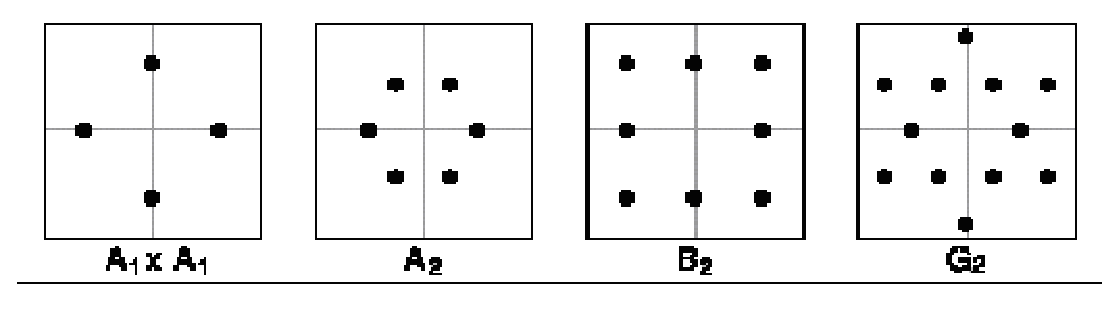
\includegraphics[width=9cm]{Root}}
\caption{秩2的根系统分类。}
\label{Root}
\end{figure}

每当 $\Phi $ 是 $V$ 中的根系统,而 $W$ 是由 $\Psi =\Phi \cap W$ 所张成的 $V$ 的子空间时,则 $\Psi $ 是在 $W$ 中的一个根系统。因此,我们对秩2的根系统的详尽列表显示在一个根系统中任意两个根的几何可能性。特别地,两个这样的根以0、30、45、60、90、120、135、150或180度的角度相交。

通常,不可约的根系统由一个族(用字母 $A$ 到 $G$ 表示)和秩(用下标 $n$ 表示)来指定。有四个无限族(\emph{infinite families}):

\begin{itemize}
\item $A_{n}\,(n\geq 1)$,其对应于特殊酉群, $%
SU(n+1)$;

\item $B_{n}\,(n\geq 2)$,其对应于特殊正交群,
$SO(2n+1)$;

\item $C_{n}\,(n\geq 3)$,其对应于辛群, $Sp(2n)
$;

\item $D_{n}\,(n\geq 4)$,其对应于特殊正交组,
$SO(2n)$,
\end{itemize}

以及五种例外情况(\emph{exceptional cases}): $E_{\mathrm{6}},E_{\mathrm{7}},E_{%
\mathrm{8}},F_{\mathrm{4}},G_{\mathrm{2}}$。

\subsubsection{邓肯图}

一个邓肯图是一个具有几种不同类型的可能边的图(参见图 \ref{Dynkin})。图的连通分量对应于 $\mathfrak{g}$ 的不可约子代数。所以一个简单的李代数的邓肯图只有一个分量。这些规则是限制性的。事实上,每个成分都只有一定的可能性,这与半单李代数的分类相对应(例如,参见文献 \cite{Conway})。

\begin{figure}[tbh]
\centerline{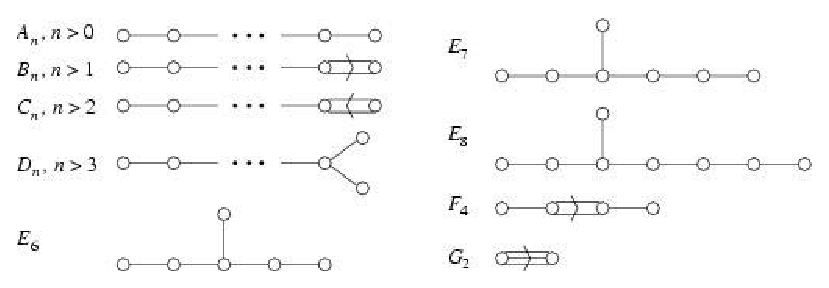
\includegraphics[width=10cm]{Dynkin}}
\caption{分类不可约根系统的问题归结为分类连通邓肯图的问题。}
\label{Dynkin}
\end{figure}

复李代数的根(\emph{roots})在一个Cartan子代数(\textit{Cartan subalgebra}) $\mathfrak{h\subset g}$中形成一个秩为 $k$ 的格(lattice),其中 $k$ 是 $\mathfrak{g}$ 的李代数秩。因此,根格(\emph{root lattice})可被认为是在 $\mathbb{R}^{k}$ 中的格。邓肯图中的顶点或节点是为每个李代数简单根(\textit{Lie algebra simple root})绘制的,其对应于根格的生成元。在两个节点 $\alpha $ 和 $\beta $ 之间,如果简单根不垂直,则绘制一条边。如果它们之间的角度为 $2\pi /3$,则绘制一条线,如果角度为 $3\pi /4$,则两条线,而如果角度为$5\pi/6$,则三条线。李代数简单根之间没有其他可能的角度。或者,简单根 $\alpha $ 和 $\beta $ 之间的线数量 $N$ 给出为
\begin{equation*}
N=A_{\alpha \beta }A_{\beta \alpha }=\frac{2\left\langle \alpha ,\beta
\right\rangle }{|\alpha |^{2}}\frac{2\left\langle \beta ,\alpha
\right\rangle }{|\beta |^{2}}=4\cos ^{2}\theta ,
\end{equation*}%
其中 $A_{\alpha \beta }=\frac{2\left\langle \alpha ,\beta \right\rangle }{ |\alpha |^{2}}$ 是在Cartan矩阵(\emph{Cartan matrix }) $(A_{\alpha \beta }) $ 中的一个条目(有关Cartan矩阵的详细信息,例如参见文献 \cite{Helgason})。在邓肯图中,一个箭头从长根绘制到短根(当角度为 $3\pi /4$ 或 $5\pi /6$ 时)。

以下是可接受的邓肯图(\textit{admissible Dynkin diagrams})的一些性质:

\begin{enumerate}
\item 通过从一个可接受图中移除一个节点而获得的图是可接受的。

\item 一个可接受的图没有循环。

\item 没有一个节点有三条以上的线连接到它。

\item 一个只有两条单线的节点序列可以被折叠,从而得到一个可接受的图。

\item 唯一有三条线的连通图有两个节点。
\end{enumerate}

一个考柯西特–邓肯图(\textit{Coxeter--Dynkin diagram}),又称考柯西特图(\textit{Coxeter graph}),其与邓肯图相同,但没有箭头。考柯西特图足以刻画代数,这可以通过列举连通图来看出。

从邓肯图中恢复简单李代数的最简单方法是首先重建其Cartan矩阵 $(A_{ij})$。第$i$个节点和第$j$个节点由 $A_{ij}A_{ji}$ 线连接。由于 $A_{ij}=0$ 当且仅当 $A_{ji}=0$ 时,否则 $A_{ij}\in \{-3,-2,-1\}$,因此很容易从他们的乘积中找到$A_{ij}$ 和 $A_{ji}$。图中的箭头指示哪个更大。例如,如果节点1和节点2之间有两条线,从节点1到节点2,则 $A_{12}=-1$ 并且 $A_{21}=-2$。

然而,值得指出的是,每个简单的李代数都可以具体构造。例如,无限族 $A_{n}$、$B_{n}$、$C_{n}$和 $D_{n}$ 对应于特殊线性李代数$ \mathfrak{gl}(n+1,\mathbb{C})$、奇数正交李代数 $\mathfrak{so} (2n+1,\mathbb{C})$、辛李代数$\mathfrak{sp}(2n,\mathbb{C})$,以及偶数正交李代数$\mathfrak{so}(2n,\mathbb{C})$。其它简单李代数被称为例外李代数(\emph{exceptional Lie algebras}),并且具有与八元数(\emph{octonions})相关的构造。

为了证明这一分类定理,人们使用根对(pairs of roots)之间的角度来编码根系统,使之成为更简单的组合对象,即邓肯图。然后邓肯图可以根据上面给出的方案进行分类。

每个根系统都有相应的邓肯图。否则,邓肯图可以通过选择一个基(\emph{base})从根系统中提取出来,这是 $\Phi $ 的一个子集 $\Delta $,它是 $V$ 的一个基,具有特殊的性质,即当在 $\Phi $ 中的每个向量在基 $\Delta $ 中写入时,或者所有都具有系数 $\geq 0$ 或者所有都是 $\leq 0$。

邓肯图的顶点对应于 $\Delta $中的向量。在每个非正交向量对之间绘制一条边;如果它们成135度角,则为双边线,如果它们成150度角,则为一条三边线。此外,双边线和三边线标记都有指向较短向量的角度符号。

尽管一个给定的根系统有一个以上的基,但Weyl群在基的集合上起传递作用。因此,根系统决定邓肯图。给定具有相同邓肯图的两个根系统,我们可以从基中的根开始匹配根,并表明这些系统实际上是相同的。

因此,根系统的分类问题可以简化为可能的邓肯图的分类问题,而不可还原根系的分类问题可以简化为连接邓肯图的分类问题。邓肯图根据基 $\Delta $ 编码 $E$ 上的内积,而这个内积必须是正定的条件,事实证明这是获得所需分类的全部条件(参见图 \ref{Dynkin})。

具体而言,各个根系统可以逐个实现,如以下段落所示:

\textbf{A$_{n}$.} 设 $V$ 为 $\mathbb{R}^{n\mathrm{+}\mathrm{1}}$ 的子空间,其坐标之和为0,并设 $\Phi $ 为 $V$ 中的向量集合,其长度为 $\sqrt{2}$,并在 $\mathbb{R}^{n\mathrm{+}\mathrm{1}}$ 中具有整数坐标。这样的向量除两个坐标等于0之外,剩余所有坐标必须具有,一个坐标等于 $1$,而另一个等于$-1$,因此总共有 $n^{\mathrm{2}}+n$ 个根。

\textbf{B$_{n}$.} 设 $V=\mathbb{R}^{n}$,并设 $\Phi $ 为包括在 $V$ 中的长度为1或 $\sqrt{2}$ 的所有整数向量。根的总数为 $2n^{\mathrm{2}}$。

\textbf{C$_{n}$:} 设 $V=\mathbb{R}^{n}$,并设 $\Phi $ 由在$V$中的长度为 $\sqrt{2}$ 的所有整数向量,以及 $2\lambda $ 形式的所有向量组成,其中 $\lambda $ 是长度为1的整数向量。根的总数为 $2n^{\mathrm{2}}$。

\textbf{D$_{n}$.} 设 $V=\mathbb{R}^{n}$,并设 $\Phi $ 由在 $V$ 中长度为 $\sqrt{2}$ 的所有整数向量组成。根的总数为$2n(n-1)$。

\textbf{E$_{n}$.} 对于 $V_{\mathrm{8}}$,设 $V=\mathbb{R}^{8}$,并设 $E_{8}$ 表示长度为 $\sqrt{2}$ 的向量集合 $\alpha $,使得 $2\alpha $ 的坐标都是整数,并且都是偶数或奇数。则$E_{\mathrm{7}}$ 可被构造为 $E_{\mathrm{8}}$ 与垂直于在 $E_{\mathrm{8}}$ 中的固定根 $\alpha $ 的向量超平面的交集。而 $E_{\mathrm{6}}$ 可被构造为与两个这样的超平面的交集,这两个超平面分别对应于根 $\alpha $ 和 $\beta $,它们既不是相互正交的也不是相互为标量倍数的。根系统 $E_{\mathrm{6}}$、$E_{\mathrm{7}}$ 和 $E_{\mathrm{8}}$ 分别具有72、126和240个根。

\textbf{F$_{4}$.} 对于 $F_{\mathrm{4}}$,设 $V=\mathbb{R}^{4}$,并设 $\Phi $ 表示长度为1或 $\sqrt{2}$ 的向量集合 $\alpha $,使得 $2\alpha $ 的坐标都是整数,并且都是偶数或奇数。在这个系统中有48个根。

\textbf{G$_{2}$.} 在 $G_{\mathrm{2}}$ 中有12个根,它们构成了六角形(\emph{hexagram})的顶点。

\subsubsection{不可约根系统}

不可约根系统对李理论中的许多相关的对象进行了分类,特别是:

\begin{enumerate}
\item 简单复李代数;

\item 简单复李群;

\item 简单连通复李群是简单模中心;
以及

\item 简单紧致李群。
\end{enumerate}

在每种情况下,根都是伴随表示的非零权重。

一个根系统也可以说是描述一个植物的根(\emph{plant's root})与相关系统。

\subsection{简单和半单李群与代数}

一个简单李群(\textit{simple Lie group})是一个李群,它也是一个简单群。这些群,以及与之密切相关的群,包括许多所谓的几何学的经典群(\emph{classical groups}),它们位于射影几何学和由 Felix Klein 的埃尔朗根程序(\textit{Erlangen programme})推导出的其它几何学的背后。它们还包括一些“例外群(\emph{exceptional groups})”,这些群是那些追求简单李群分类的人首先发现的。这些例外群在数学的其它分支中解释了许多例外的示例和配置。特别是有限简单群的分类取决于事先对“例外”可能性的彻底先验知识。

简单李群的完整列表是半单李群和可简约群及其表示理论的基础。事实证明,这不仅是紧致李群理论(及其表示理论)的一个主要扩展,而且在数学物理学中具有基本意义。

使用复数简单李代数的先验分类对这样的群进行分类。已经证明,一个简单的李群具有一个简单李代数,一旦它被复数化(即,制成一个复向量空间而不是一个实向量空间),它就会出现在给定的列表上。这将分类简化为两个进一步的事项。

例如,群 $SO(p,q,\mathbb{R})$ 和 $SO(p+q,\mathbb{R})$ 产生不同的实李代数,但具有相同的邓肯图。一般来说,同一复数李代数可能有不同的实数形式(\emph{real forms})。

其次,李代数仅唯一地确定包含李群$G$的特征的分量的单连通的(泛)覆盖 $G^{\ast }$。很可能 $G^{\ast }$ 实际上不是一个简单群,例如具有一个非平凡的中心。因此,我们必须通过计算$G$的基本群(一个阿贝尔群:一个李群是一个$H$空间)来担心全局拓扑。这是由Elie Cartan完成的。

例如,以偶数维度的特殊正交群为例。由于$-I$是一个位于中心的标量矩阵,这些群实际上不是简单群;并且有一个双折叠的自旋覆盖,它们也不是简单地连通在一起。在上面的表示法中,它们“位于” $G^{\ast }$ 和 $G$ 之间。

回想一下,半单模(\emph{semisimple module})是一个其每个子模都是直和的模。特别地,一个半单表示(\textit{semisimple representation})是完全可简约的,即,是不可约表示的直和(在下降链条件下)。类似地,当每个对象都具有相应的性质时,人们可以将阿贝尔范畴称为半单范畴。此外,一个半单环是一个它作为在它自身上的模的半单环。

一个半单矩阵(\emph{semisimple matrix})在包含其条目的任意代数闭域上是可对角化的。在实践中,这意味着它有一个对角矩阵作为其约当标准型。

当一个李代数(\emph{Lie algebra}) $\mathfrak{g}$ 被称为是半单的(\emph{semisimple}),当它是简单李代数(\emph{simple Lie algebras})的一个直和时,即非平凡李代数 $\mathfrak{L}$ ,其唯一理想是 $\{0\}$ 和 $\mathfrak{L}$ 本身。一个等价条件是该 \textit{Killing form}
\begin{equation*}
\mathcal{B}(X,Y)=\limfunc{Tr}(Ad(X)\,Ad(Y))
\end{equation*}
是非退化的 \cite{Schafer}。可以证明以下性质对于特征 $0$ 域上的一个有限维代数 $\mathfrak{L}$ 是等价的:

1. $\mathfrak{L}$ 是半单的。

2. $\mathfrak{L}$ 没有非零阿贝尔理想。

3. $\mathfrak{L}$ 具有零根数(radical) (根数是最大的可解理想)。

4. $\mathfrak{L}$ 的每个表示都是完全可简约的,即是一个不可约表示的加和。

5. $\mathfrak{L}$ 是简单李代数的一个(有限)直积(如果一个李代数不是阿贝尔代数并且没有非零理想,则称为简单李代数)。

一个连通李群(\textit{connected Lie group})被称为半单的(\emph{semisimple}),当其李代数为半单时;并且代数群也是如此。一个半单李代数、李群,或在特征为$0$中的代数群,它们的每一个有限维表示都是半单的,即完全可简约的,但反之则不成立。此外,在特征 $p>0$中,半单李群和李代数具有非半单的有限维表示。如果半单李群或李代数的元素在每个有限维表示中的象在矩阵意义上是半单的,则它本身就是半单的。

每个半单李代数 $\mathfrak{g}$ 都可以通过其邓肯图来分类 \cite{Helgason}。

\section{李群的几个经典例子}

\subsection{伽利略群}

伽利略群(\textit{Galilei group})是连通那些在牛顿力学中被称为“惯性帧”的笛卡尔系统的空间和时间变换群。两种这样的帧之间最一般的关系如下。在惯性帧$ S^{\prime }$中的时间尺度的原点可能会与在$S$中的时间标尺的原点发生偏移;在 $S^{\prime }$ 中笛卡尔轴的方向可能与在$S$中的方向不同;在 $S^{\prime }$ 中的笛卡尔帧的原点$O$可以以均匀的速度相对于在$S$中的原点$O$移动。从$S$到 $S^{\prime }$ 的转换涉及十个参数;因此伽利略群是十元参数群。在伽利略–牛顿相对论中固有的基本假设是存在绝对时间尺度,因此,两个不同的“惯性观测者”使用的时间变量可能不同的唯一方式是,其中一个观测者的时间零点可能会相对于另一个观者的时间点发生偏移(例如参见文献 \cite{Arnold,GaneshSprBig,GaneshADG})。

伽利略时空结构包括以下三种要素:

\begin{enumerate}
\item 世界(\emph{World}),作为4D仿射空间 $A^{4}$。$A^{4}$ 的点被称为世界点(\emph{world points})或事件(\emph{events})。世界 $A^{4}$ 的平行转换形成线性(即欧几里得)空间 $\mathbb{R}^{4}$。

\item 时间(\emph{Time}),作为线性映射 $t:\mathbb{R}^{4}\rightarrow \mathbb{R}$,将世界的线性空间的平行转换到实时“时间轴”上。从事件 $a\in A^{4}$ 到 $b\in A^{4}$ 的时间间隔称为数字 $t(b-a)$;如果 $t(b-a)=0$ ,则事件 $a$ 和 $b$ 称为同步。所有相互同步事件的集合包括3D仿射空间 $A^{3}$,其是世界 $A^{4}$ 的子空间。映射 $t$ 的内核包括 $A^{4}$ 的并行转换,它将任意(和每个)事件转换为同步事件;它是空间 $\mathbb{R}^{4}$ 的线性3D子空间 $\mathbb{R}^{3}$。

\item 距离(度量),在同步事件之间,
\begin{equation*}
\rho (a,b)=\parallel a-b\parallel ,\qquad \text{for all}\quad a,b\in \mathop %
A\nolimits^{3},
\end{equation*}%
由 $\mathbb{R}^{3}$ 中的标量乘积给出。该距离将同步事件的任意空间转换为众所周知的3D欧几里得空间 $E^{3}$。
\end{enumerate}

该空间 $A^4$,加上伽利略时空结构,被称为伽利略空间。伽利略群是伽利略空间的所有可能变换的群,保持其结构。伽利略群的元素称为伽利略变换。因此,伽利略变换是世界 $A^4$ 的仿射变换,保留了同步事件之间的时间间隔和距离。

时间轴与具有固定欧几里得结构的3D线性空间 $\mathbb{R}^{3}$ 的直积 $\mathbb{R}\times \mathbb{R}^{3}$,具有自然的伽利略结构。它被称为伽利略坐标系统。

\subsection{一般线性群}

$\mathbb{R}^{n}$ 到 $\mathbb{R}^{n}$ 的线性同构群是维度为 $n^{2}$ 的李群,被称为一般线性群(\textit{general linear group}),并被表示为 $Gl(n,\mathbb{R})$。它是一个光滑流形,因为它是 $\mathbb{R}^{n}$ 到 $\mathbb{R}^{n}$ 的所有线性映射的向量空间 $L(\mathbb{R}^{n},\mathbb{R}^{n})$ 的子集,因为 $Gl(n,\mathbb{R})$ 是 $\mathbb{R}\backslash \{0\}$ 在 $L(\mathbb{R}^{n},\mathbb{R}^{n})$ 到 $\mathbb{R}$ 的连续映射 $ A\mapsto \det A$ 下的逆象(inverse image)。该群的运算是组合(例如参见文献 \cite{Arnold,Abraham,GaneshSprBig,GaneshADG})。
\begin{equation*}
(A,B)\in Gl(n,\mathbb{R})\times Gl(n,\mathbb{R})\mapsto A\circ B\in Gl(n,%
\mathbb{R})
\end{equation*}%
并且其逆映射为
\begin{equation*}
A\in Gl(n,\mathbb{R})\mapsto A^{-1}\in Gl(n,\mathbb{R}).
\end{equation*}%
如果我们在 $\mathbb{R}^{n}$ 中选择一个基,我们可以用一个可逆的 $(n\times n)$ 矩阵来表示每个元素 $ A\in Gl(n,\mathbb{R})$。则群运算是矩阵乘法,逆运算是矩阵逆运算。其特征是特征矩阵 $I_{n}$。群运算是光滑的,因为矩阵的乘积和逆的公式在矩阵分量中是光滑的。

群 $Gl(n,\mathbb{R})$ 的李代数是 $\mathfrak{gl}(n)$,即 $\mathbb{R}^{n}$的所有线性变换的向量空间 $L(\mathbb{R}^{n},\mathbb{R}^{n})$,具有交换子(commutator)括号
\begin{equation*}
\lbrack A,B]=AB-BA.
\end{equation*}%
对于每个 $A\in L(\mathbb{R}^{n},\mathbb{R}^{n})$,
\begin{equation*}
\gamma _{A}:t\in \mathbb{R\mapsto }\gamma _{A}(t)=\sum_{i=0}^{\infty }\frac{%
t^{i}}{i!}A^{i}\in Gl(n,\mathbb{R})
\end{equation*}%
是 $Gl(n,\mathbb{R})$ 的单参数子群,因为
\begin{equation*}
\gamma _{A}(0)=I\qquad \text{and\qquad }\dot{\gamma}_{A}(t)=\sum_{i=0}^{%
\infty }\frac{t^{i-1}}{(i-1)!}A^{i}=\gamma _{A}(t)\,A
\end{equation*}
因此 $\gamma _{A}$ 是左不变向量–场 $X_{A}$ 的积分曲线。因此,指数映射给出为
\begin{equation*}
\exp :A\in L(\mathbb{R}^{n},\mathbb{R}^{n})\mapsto \exp (A)\equiv \mathrm{e}%
^{A}=\gamma _{A}(1)=\sum_{i=0}^{\infty }\frac{A^{i}}{i!}\in Gl(n,\mathbb{R}).
\end{equation*}

对于每个 $A\in Gl(n,\mathbb{R})$ ,对应的伴随映射
\begin{equation*}
Ad_{A}:L(\mathbb{R}^{n},\mathbb{R}^{n})\rightarrow L(\mathbb{R}^{n},\mathbb{R%
}^{n})
\end{equation*}%
由下式给出为
\begin{equation*}
Ad_{A}B=A\cdot B\cdot A^{-1}.
\end{equation*}

\subsection{人类/类人生物力学中的旋转李群}

在每个旋转机器人或(滑膜)人类关节处的局部运动学被定义为一个在欧几里得空间 $\mathbb{R}^{n}$ 上的一个$n$D约束旋转李群 $SO(n)$ 的群作用(\emph{group action})。特别是,在单轴人体关节(圆柱形或铰链关节(\emph{hinge joints}),如膝盖和肘部)中有一个 $SO(2)$ 群作用,在三轴人体关节中(球形或球窝关节(\emph{ball--and--socket joints}),如臀部、肩部、颈部、手腕和脚踝)有一个 $SO(3)$ 群作用。在这两种情况下,$SO(n)$ 以其旋转算子作用于父机体段的外部笛卡尔坐标的向量 $x=\{x^{\mu }\},\,(i=1,2,3)$,同时取决于$n$维群参数上的向量 $q=\{q^{s}\},\,(s=1,\cdots ,n)$,即关节角度(参见文献 \cite{SIAM,GaneshSprSml,GaneshSprBig,GaneshADG})。

每个关节旋转 $R\in SO(n)$ 定义一个映射
\begin{equation*}
R:x^{\mu }\mapsto \dot{x}{}^{\mu }, \qquad R(x^{\mu },q^{s})=R_{q^{s}}x^{\mu
},
\end{equation*}
是 $R_{q^{s}}\in SO(n)$ 是关节群算子。这些旋转的 $n$ 维无穷小生成元的向量 $v=\{v_{s}\},\,(s=1,\cdots ,n)$,即关节角速度,给出为
\begin{equation*}
v_{s}=-\left[\frac{\partial R(x^{\mu },q^{s})}{\partial q^{s}}\right]_{q=0}%
\frac{\partial }{\partial x^{\mu }}
\end{equation*}
其构成对应于关节旋转群 $SO(n)$ 的 $n$D 李代数 $\mathfrak{so}(n)$。相反,表示 $SO(n)$ 的一个单参数子群的每个关节群算子 $R_{q^{s}}$ 被定义为相应关节群生成元 $v_{s}$ 的指数映射
\begin{equation*}
R_{q^{s}}=\exp (q^{s}v_{s})
\end{equation*}
该指数映射表示在关节群–参数空间 $\{q^{s}\}$ 中关节算子微分方程的一个解
\begin{equation*}
\frac{dR_{q^{s}}}{dq^{s}}=v_{s}R_{q^{s}}.
\end{equation*}

\subsubsection{关节旋转的单轴群}

单轴关节旋转为在单一笛卡尔平面中围绕垂直轴,例如 $xy$ 平面所围绕的 $z$ 轴,旋转一个内部关节角度 $\theta$ ,导致关节坐标的变换为:
\begin{equation*}
x^{\prime }=x\cos \theta -y\sin \theta ,\qquad y^{\prime }=x\sin \theta
+y\cos \theta .
\end{equation*}
这样,关节 $SO(2)$ 群给出为
\begin{equation*}
SO(2)=\left\{ R_{\theta }=\left(
\begin{array}{cc}
\cos \theta & -\sin \theta \\
\sin \theta & \cos \theta%
\end{array}%
\right) |\theta \in \lbrack 0,2\pi ]\right\},
\end{equation*}%
其以规范的方式作用于欧几里得平面 $\mathbb{R}^{2}$,通过下式
\begin{equation*}
SO(2)=\left( \left(
\begin{array}{cc}
\cos \theta & -\sin \theta \\
\sin \theta & \cos \theta%
\end{array}%
\right) ,\left(
\begin{array}{c}
x \\
y%
\end{array}%
\right) \right) \longmapsto \left(
\begin{array}{cc}
x\cos \theta & -y\sin \theta \\
x\sin \theta & y\cos \theta%
\end{array}%
\right).
\end{equation*}
其关联的李代数 $\mathfrak{so}(2)$ 给出为
\begin{equation*}
\mathfrak{so}(2)=\left\{ \left(
\begin{array}{cc}
0 & -t \\
t & 0%
\end{array}%
\right) |t\in \mathbb{R}\right\} ,
\end{equation*}%
由于曲线 $\gamma _{\theta }\in SO(2)$ 由下式给出
\begin{equation*}
\gamma _{\theta }:t\in \mathbb{R}\longmapsto \gamma _{\theta }(t)=\left(
\begin{array}{cc}
\cos t\theta & -\sin t\theta \\
\sin t\theta & \cos t\theta%
\end{array}%
\right) \in SO(2),
\end{equation*}%
其通过特征式 $I_{2}=\left(
\begin{array}{cc}
1 & 0 \\
0 & 1%
\end{array}%
\right) $ 给出,并然后有
\begin{equation*}
\left. \frac{d}{dt}\right\vert _{t=0}\gamma _{\theta }(t)=\left(
\begin{array}{cc}
0 & -\theta \\
\theta & 0%
\end{array}%
\right) ,
\end{equation*}%
所以这个 $I_{2}$ 是 $\mathfrak{so}(2)$ 的一个基,由于 $\dim \left(
SO(2)\right) =1$。

指数映射(\emph{exponential map}) $\exp :\mathfrak{so}(2)\rightarrow SO(2)$ 给出为
\begin{equation*}
\exp \left(
\begin{array}{cc}
0 & -\theta \\
\theta & 0%
\end{array}
\right) =\gamma _{\theta }(1)=\left(
\begin{array}{cc}
\cos t\theta & -\sin t\theta \\
\sin t\theta & \cos t\theta%
\end{array}
\right).
\end{equation*}

$SO(2)$ 在 $\mathbb{R}^{2}$ 上作用的无穷小生成元(\emph{infinitesimal generator}),即关节角速度 $v$,给出为
\begin{equation*}
v=-y\frac{\partial }{\partial x}+x\frac{\partial }{\partial y},
\end{equation*}
由于
\begin{equation*}
v_{\mathbb{R}^{2}}\left( x,y\right) =\left. \frac{d}{dt}\right\vert
_{t=0}\exp (tv)\left( x,y\right) =\left. \frac{d}{dt}\right\vert
_{t=0}\left(
\begin{array}{cc}
\cos tv & -\sin tv \\
\sin tv & \cos tv%
\end{array}%
\right) \left(
\begin{array}{c}
x \\
y%
\end{array}%
\right) .
\end{equation*}

动量映射(\emph{momentum map}) $J:T^{\ast }\mathbb{R}^{2}\rightarrow \mathbb{R}$,关联到在 $T^{\ast }\mathbb{R}^{2}\simeq \mathbb{R}^{4}$ 上的 $SO(2)$ 的提升作用,给出为
\begin{eqnarray*}
J\left( x,y,p_{1},p_{2}\right) &=&xp_{y}-yp_{x},\qquad \text{since} \\
J\left( x,y,p_{x},p_{y}\right) (\xi ) &=&(p_{x}dx+p_{y}dy)(v_{\mathbb{R}%
^{2}})=-vp_{x}y+-vp_{y}x.
\end{eqnarray*}

李群 $SO(2)$ 通过下式作用于辛流形 $(\mathbb{R}%
^{4},\omega =dp_{x}\wedge dx+dp_{y}\wedge dx)$  
\begin{eqnarray*}
&&\qquad\phi \left( \left(
\begin{array}{cc}
\cos \theta & -\sin \theta \\
\sin \theta & \cos \theta%
\end{array}
\right) ,\left( x,y,p_{x},p_{y}\right) \right) \\
&=&\left( x\cos \theta -y\sin \theta ,\,x\sin \theta +y\cos \theta
,\,p_{x}\cos \theta -p_{y}\sin \theta ,\,p_{x}\sin \theta +p_{y}\cos \theta
\right) .
\end{eqnarray*}%
\bigbreak

\subsubsection{关节旋转的三轴群}

类人关节旋转的三轴 $SO(3)$ 群取决于三个参数,即欧拉关节角度 $q^{i}=(\varphi ,\psi ,\theta )$,定义了围绕放置在关节枢轴点的笛卡尔三轴坐标 $(x,y,z)$ 的旋转。每个欧拉角都定义在受约束范围 $(-\pi ,\pi )$ 内,因此关节群空间是半径为 $\pi $ 的约束球面 (参见文献 \cite{SIAM,GaneshSprSml,GaneshSprBig,GaneshADG})。

设 $G=SO(3)=\{A\in \mathcal{M}_{3\times 3}(\mathbb{R}):A^{t}A=I_{3},\det
(A)=1\}$ 是在 $\mathbb{R}^{3}$ 中的旋转群。它是一个李群,并且 $\dim(G)=3$。让我们隔离它的单参数关节子群,即考虑有限关节旋转的三个算子 $R_{\varphi
},R_{\psi },R_{\theta }\in SO(3)$,给出为
\begin{equation*}
R_{\varphi } =\left[
\begin{array}{ccc}
1 & 0 & 0 \\
0 & \cos \varphi & -\sin \varphi \\
0 & \sin \varphi & \cos \varphi%
\end{array}
\right] , ~~ R_{\psi } =\left[
\begin{array}{ccc}
\cos \psi & 0 & \sin \psi \\
0 & 1 & 0 \\
-\sin \psi & 0 & \cos \psi%
\end{array}
\right] , ~~ R_{\theta } =\left[
\begin{array}{ccc}
\cos \theta & -\sin \theta & 0 \\
\sin \theta & \cos \theta & 0 \\
0 & 0 & 1%
\end{array}
\right]
\end{equation*}%
\noindent 它们分别对应于绕 $x$ 轴旋转一个角度$\varphi$,绕 $y$ 轴旋转一个角度 $\psi$,绕 $z$ 轴旋转一个角度 $\theta $。

总的三轴关节旋转 $A$ 定义为上述单参数旋转 $R_{\varphi },R_{\psi },R_{\theta }$ 的乘积,即 $A=R_{\varphi }\cdot R_{\psi }\cdot R_{\theta }$ 等于\footnote{%
注意,这个乘积是非交换的,所以它确实取决于乘法的顺序。} 
\begin{equation*}
A=\left[
\begin{array}{ccc}
\cos \psi \cos \varphi -\cos \theta \sin \varphi \sin \psi & \cos \psi \cos
\varphi +\cos \theta \cos \varphi \sin \psi & \sin \theta \sin \psi \\
-\sin \psi \cos \varphi -\cos \theta \sin \varphi \sin \psi & -\sin \psi
\sin \varphi +\cos \theta \cos \varphi \cos \psi & \sin \theta \cos \psi \\
\sin \theta \sin \varphi & -\sin \theta \cos \varphi & \cos \theta%
\end{array}
\right] .
\end{equation*}
然而,这些矩阵积的顺序很重要:不同的顺序积给出不同的结果,因为矩阵积是非交换积(\textit{noncommutative product})。这就是为什么汉密尔顿的四元数(\textit{quaternions})\footnote{%
回想一下,汉密尔顿四元数(\textit{quaternions}) $\mathbb{H}$ 的集合表示复数 $\mathbb{C}$ 集合的扩展。我们可以计算围绕单位向量 $\mathbf{u}$ 的旋转角度 $\theta $。计算此旋转的四元数 $q$ 为
\begin{equation*}
q=\left( \cos \frac{\theta }{2}~,~u\sin \frac{\theta }{2}\right) .
\end{equation*}%
}今天通常被用来参数化 $SO(3)$ 群的原因,特别是在3D计算机图形学领域。

单参数旋转 $R_{\varphi },R_{\psi },R_{\theta }$ 定义在 $SO(3)$ 中从 $I_{3}={\small \left(
\begin{array}{ccc}
1 & 0 & 0 \\
0 & 1 & 0 \\
0 & 0 & 1%
\end{array}
\right)}$ 开始的曲线。它们在 $\varphi =0,\psi =0$ 和 $\theta =0$ 中的导数属于相关的正切李代数(\emph{tangent Lie algebra}) $\mathfrak{so}(3)$。也就是说,关节旋转的相应无穷小生成元 -- 关节角速度 $v_{\varphi },v_{\psi },v_{\theta }\in \mathfrak{so}(3)$ -- 分别给出为
\begin{eqnarray*}
v_{\varphi } &=&{\small \left[
\begin{array}{ccc}
0 & 0 & 0 \\
0 & 0 & -1 \\
0 & 1 & 0%
\end{array}%
\right]} =-y\frac{\partial }{\partial z}+z\frac{\partial }{\partial y}%
,\qquad v_{\psi }={\small \left[
\begin{array}{ccc}
0 & 0 & 1 \\
0 & 0 & 0 \\
-1 & 0 & 0%
\end{array}%
\right]} =-z\frac{\partial }{\partial x}+x\frac{\partial }{\partial z}, \\
v_{\theta } &=&{\small \left[
\begin{array}{ccc}
0 & -1 & 0 \\
1 & 0 & 0 \\
0 & 0 & 0%
\end{array}%
\right]} =-x\frac{\partial }{\partial y}+y\frac{\partial }{\partial x}.
\end{eqnarray*}
此外,这些元素是线性独立的,并因此
\begin{equation*}
\mathfrak{so}(3)=\left\{ \left[
\begin{array}{ccc}
0 & -a & b \\
a & 0 & -\gamma \\
-b & \gamma & 0%
\end{array}
\right] |a,b,\gamma \in \mathbb{R}\right\}.
\end{equation*}
该李代数 $\mathfrak{so}(3)$ 通过与每个 $v=(v_{\varphi },v_{\psi },v_{\theta })\in \mathbb{R}^{3} $ 相关联而与 $\mathbb{R}^{3}$ 标识,矩阵 $v\in \mathfrak{so}(3)$ 由 $v={\small \left[
\begin{array}{ccc}
0 & -a & b \\
a & 0 & -\gamma \\
-b & \gamma & 0%
\end{array}
\right]}$ 给出。则我们有以下标识:

\begin{enumerate}
\item $\widehat{u\times v}=[\hat{u},v]$; and

\item $u\cdot v=-\frac{1}{2}\limfunc{Tr}(\hat{u}\cdot v)$.
\end{enumerate}

指数映射 $\exp :\mathfrak{so}(3)\rightarrow SO(3)$ 由罗德里格斯关系式(\emph{Rodrigues relation})给出为
\begin{equation*}
\exp (v)=I+\frac{\sin \left\Vert v\right\Vert }{\left\Vert v\right\Vert }v+%
\frac{1}{2}\left( \frac{\sin \frac{\left\Vert v\right\Vert }{2}}{\frac{%
\left\Vert v\right\Vert }{2}}\right) ^{2}v^{2}
\end{equation*}
其中模 $\left\Vert v\right\Vert $ 给出为
\begin{equation*}
\left\Vert v\right\Vert =\sqrt{(v^{1})^{2}+(v^{2})^{2}+(v^{3})^{2}}.
\end{equation*}

对偶的余切李代数(\emph{cotangent Lie algebra}) $\mathfrak{so}(3)^{\ast }$ 包括三个关节角动量 $p_{\varphi },p_{\psi },p_{\theta}\in \mathfrak{so}(3)^{\ast }$,由关节速度 $v$ 乘以相应的转动惯量得出。

注意,$SO(3)$ 旋转的参数化是许多力学理论与应用领域不断研究和开发的主题,例如刚体、结构和多体动力学、机器人、航天器姿态动力学、导航、图像处理等领域。

\subsubsection{沉重的顶端}

考虑一个刚体在重力作用下以一个固定点移动。这个问题仍然有一个构型空间 $SO(3)$,但对称群只是圆群 $S^{1}$,由围绕重力方向的旋转组成。有人说重力打破了从 $SO(3)$ 到 $S^{1}$ 的对称性。这一次,消除 $S^{1}$ 对称性神秘地导致 $\mathbb{R}^{3}$ 的刚性运动的更大的欧几里得群 $SE(3)$。相反,我们可以从 $SE(3)$ 开始作为刚体的构型空间,并“减少”平移,以达到 $SO(3)$ 作为的构型空间。在重力场中具有固定点的刚体的运动方程给出了哈密顿系统的一个有趣的例子。底层李代数包括在 $\mathbb{R}^{3}$ 中无穷小的欧几里得运动的代数(参见文献 \cite{Arnold,Abraham,GaneshSprBig,GaneshADG})。

我们开始的基本相空间还是 $T^{\ast }SO(3)$,由欧拉角及其共轭动量参数化。在这些变量中,方程是正则哈密顿形式。然而,重力的存在打破了对称性,系统不再是 $SO(3)$ 不变的,因此不能完全用机体角动量 $p$ 来表示。我们还需要跟踪 $\Gamma $,即从机体上看的“重力方向”。这是由 $\Gamma =A^{-1}k$ 定义的,其中 $k$ 指向上方,并且 $A$ 是 $SO(3)$ 的元素,用以描述物体当前构型。这些运动方程组为
\begin{eqnarray*}
\dot{p}_{1} &=&\frac{I_{2}-I_{3}}{I_{2}I_{3}}p_{2}p_{3}+Mgl(\Gamma ^{2}\chi
^{3}-\Gamma ^{3}\chi ^{2}), \\
\dot{p}_{2} &=&\frac{I_{3}-I_{1}}{I_{3}I_{1}}p_{3}p_{1}+Mgl(\Gamma ^{3}\chi
^{1}-\Gamma ^{1}\chi ^{3}), \\
\dot{p}_{3} &=&\frac{I_{1}-I_{2}}{I_{1}I_{2}}p_{1}p_{2}+Mgl(\Gamma ^{1}\chi
^{2}-\Gamma ^{2}\chi ^{1}), \\
&&\text{and\qquad }\dot{\Gamma}\;=\;\Gamma \times \Omega ,
\end{eqnarray*}%
其中 $\Omega $ 是机体的角速度向量,$I_{1},I_{2},I_{3}$ 是机体的主要转动惯量,$M$ 是机体的质量,$g$ 是重力加速度,$\chi $ 是连接固定点和机体质心的线段上的机体固定单位向量,并且 $l$ 是该线段的长度。

\subsection{刚体运动的欧几里得群}

在本小节中,我们分别描述在2D和3D中的在经典力学中两个最重要的李群,即 $SE(2)$ 和 $SE(3)$ (参见文献 \cite{Marsden,GaneshSprBig,GaneshADG})。

\subsubsection{在平面中的特殊欧几里得群 $SE(2)$}

\label{SE(2)}

单轴人体关节的运动自然地由在平面中的特殊欧几里得群(\emph{special Euclidean group in the plane}) $SE(2)$ 建模。它由形式为 $Az+a$ 的 $\mathbb{R}^{2}$ 的所有变换组成,其中 $z,a\in \mathbb{R}^{2}$,并且% 
\begin{equation*}
A\in SO(2)=\left\{ \text{matrices of the form }\left(
\begin{array}{cc}
\cos \theta & -\sin \theta \\
\sin \theta & \cos \theta%
\end{array}%
\right) \right\} .
\end{equation*}%
换句话说,群 $SE(2)$ 由以下形式的矩阵组成:\newline
$(R_{\theta },a) ={\small \left(
\begin{array}{cc}
R_{\theta } & a \\
0 & I%
\end{array}%
\right)}$,其中 $a\in \mathbb{R}^{2}$ 和 $R_{\theta }$ 是旋转矩阵:\newline
$R_{\theta }={\small \left(
\begin{array}{cc}
\cos \theta & -\sin \theta \\
\sin \theta & \cos \theta%
\end{array}%
\right)}$,而 $I$ 是 $3\times 3$ 单位矩阵。其逆矩阵 $%
\left( R_{\theta },a\right) ^{-1}$ 给出为%
\begin{equation*}
\left( R_{\theta },a\right) ^{-1}=\left(
\begin{array}{cc}
R_{\theta } & a \\
0 & I%
\end{array}%
\right) ^{-1}=\left(
\begin{array}{cc}
R_{-\theta } & -R_{-\theta }a \\
0 & I%
\end{array}%
\right) .
\end{equation*}%
$SE(2)$ 的李代数 $\mathfrak{se}(2)$ 由 $3\times 3$ 块状矩阵组成,其形式为% 
\begin{equation*}
\left(
\begin{array}{cc}
-\xi J & v \\
0 & 0%
\end{array}%
\right) ,\qquad \text{其中}\qquad J=\left(
\begin{array}{cc}
0 & 1 \\
-1 & 0%
\end{array}%
\right), \qquad (J^{T}=J^{-1}=-J),
\end{equation*}%
具有通常的交换子括号。如果我们标识 $\mathfrak{se}(2)$ 与 $%
\mathbb{R}^{3}$ 通过同构%
\begin{equation*}
\left(
\begin{array}{cc}
-\xi J & v \\
0 & 0%
\end{array}%
\right) \in \mathfrak{se}(2)\longmapsto (\xi ,v)\in \mathbb{R}^{3},
\end{equation*}%
则李代数括号的表达式变为

\begin{equation*}
\lbrack (\xi ,v_{1},v_{2}),(\zeta ,w_{1},w_{2})]=(0,\zeta v_{2}-\xi
w_{2},\xi w_{1}-\zeta v1)=(0,\xi J^{T}w-\zeta J^{T}v),
\end{equation*}%
其中 $v=(v_{1},v_{2})$ 并且 $w=(w_{1},w_{2})$。

以下的伴随群作用(\emph{adjoint group action})%
\begin{equation*}
\left( R_{\theta },a\right) \left(
\begin{array}{cc}
R_{\theta } & a \\
0 & I%
\end{array}%
\right) \qquad \text{其在}\qquad (\xi ,v)=\left(
\begin{array}{cc}
-\xi J & v \\
0 & 0%
\end{array}%
\right)
\end{equation*}%
之上,由群共轭(\emph{group conjugation})给出为%
\begin{equation*}
\left(
\begin{array}{cc}
R_{\theta } & a \\
0 & I%
\end{array}%
\right) \left(
\begin{array}{cc}
-\xi J & v \\
0 & 0%
\end{array}%
\right) \left(
\begin{array}{cc}
R_{-\theta } & -R_{-\theta }a \\
0 & I%
\end{array}%
\right) =\left(
\begin{array}{cc}
-\xi J & \xi Ja+R_{\theta }v \\
0 & 0%
\end{array}%
\right) ,
\end{equation*}%
或者,在以下坐标中,
\begin{equation}
Ad_{\left( R_{\theta },a\right) }(\xi ,v)=(\xi ,\xi Ja+R_{\theta }v).
\label{adse2}
\end{equation}

在证明方程(\ref{adse2})中,我们使用特征式 $R_{\theta }J=JR_{\theta }$。通过乘积的迹给出的非退化配对,将对偶代数 $\mathfrak{se}(2)^{\ast }$,用形式为 $\left(
\begin{array}{cc}
\frac{\mu }{2}J & 0 \\
\alpha & 0%
\end{array}%
\right)$ 的矩阵识别。因此,$\mathfrak{se}(2)^{\ast }$ 通过以下方式与 $\mathbb{R}^{3}$ 同构%
\begin{equation*}
\left(
\begin{array}{cc}
\frac{\mu }{2}J & 0 \\
\alpha & 0%
\end{array}%
\right) \in \mathfrak{se}(2)^{\ast }\longmapsto (\mu ,\alpha )\in \mathbb{R}%
^{3},
\end{equation*}%
因此,在这些坐标中,$\mathfrak{se}(2)^{\ast }$ 和 $\mathfrak{se}(2)$ 变为%
\begin{equation*}
\left\langle (\mu ,\alpha ),(\xi ,v)\right\rangle =\mu \xi +\alpha \cdot v,
\end{equation*}%
也就是在 $\mathbb{R}^{3}$ 中通常的点积。因此,共轭群作用(\emph{coadjoint group action})给出为%
\begin{equation}
Ad_{\left( R_{\theta },a\right) ^{-1}}^{\ast }(\mu ,\alpha )=(\mu -R_{\theta
}\alpha \cdot Ja+R_{\theta }\alpha ).  \label{ad*se2}
\end{equation}

公式(\ref{ad*se2})表明,如果 $\alpha \neq 0$ 连同在 $\mu$ 轴上的点一起,则协伴随轨道是圆柱体 $T^{\ast }S_{\alpha }^{1}=\{(\mu ,\alpha )|\left\Vert \alpha \right\Vert=\text{const}\}$。规范余切丛投影 $\pi :T^{\ast }S_{\alpha
}^{1}\rightarrow S_{\alpha }^{1}$ 定义为 $\pi (\mu ,\alpha )=\alpha$。

\subsubsection{在 3D 空间中的特殊欧几里得群 $SE(3)$}

\label{SE(3)}

人类生物动力学中最常见的群结构是在 3D 空间中的特殊欧几里得群(\emph{special Euclidean group in 3D space}),$SE(3)$。简而言之,欧几里得 $SE(3)$ 群被定义为 3D 旋转和 3D 平移的半直(非交换)积,$SE(3):=SO(3)\rhd \mathbb{R}^{3}$ (参见文献 \cite{Marsden,GaneshSprBig,GaneshADG})。其最重要的子群如下:\newline

{{\frame{$%
\begin{array}{cc}
\mathbf{Subgroup} & \mathbf{Definition} \\ \hline
\begin{array}{c}
SO(3),\text{ group of rotations} \\
\text{in 3D (a spherical joint)}%
\end{array}
&
\begin{array}{c}
\text{Set of all proper orthogonal } \\
3\times 3-\text{rotational matrices}%
\end{array}
\\ \hline
\begin{array}{c}
SE(2),\text{ special Euclidean group} \\
\text{in 2D (all planar motions)}%
\end{array}
&
\begin{array}{c}
\text{Set of all }3\times 3-\text{matrices:} \\
\left[
\begin{array}{ccc}
\cos \theta & \sin \theta & r_{x} \\
-\sin \theta & \cos \theta & r_{y} \\
0 & 0 & 1%
\end{array}%
\right]%
\end{array}
\\ \hline
\begin{array}{c}
SO(2),\text{ group of rotations in 2D} \\
\text{subgroup of }SE(2)\text{--group} \\
\text{(a revolute joint)}%
\end{array}
&
\begin{array}{c}
\text{Set of all proper orthogonal } \\
2\times 2-\text{rotational matrices} \\
\text{ included in }SE(2)-\text{group}%
\end{array}
\\ \hline
\begin{array}{c}
\mathbb{R}^{3},\text{ group of translations in 3D} \\
\text{(all spatial displacements)}%
\end{array}
& \text{Euclidean 3D vector space}%
\end{array}%
$}}} \bigskip

\paragraph{李群 $SE(3)$ 及其李代数}

$SE(3)$ 的一个元素是一对 $(A,a)$,其中 $A\in SO(3)$ 并且 $a\in \mathbb{R}^{3}$。$SE(3)$ 在 $\mathbb{R}^{3}$ 上的作用是先旋转 $A$,然后通过向量 $a$ 进行平移,并且其表达式为
\begin{equation*}
(A,a)\cdot x=Ax+a.
\end{equation*}
使用此公式,人们可以看到,对于 $A,B\in SO(3)$ 和 $a,b\in \mathbb{R}^{3}$,$SE(3)$中的乘法与求逆给出为
\begin{equation*}
(A,a)(B,b)=(AB,Ab+a)\qquad \text{and\qquad }(A,a)^{-1}=(A^{-1},-A^{-1}a).
\end{equation*}
其特征元素为 $(l,0)$。

欧几里得群 $SE(3)$ 的李代数是 $\mathfrak{se}(3)=\mathbb{R}^{3}\times \mathbb{R}^{3}$,具有李括号为
\begin{equation}
\lbrack (\xi ,u),(\eta ,v)]=(\xi \times \eta ,\xi \times v-\eta \times u).
\label{lbse3}
\end{equation}

欧几里得群的李代数具有一种结构,这是所谓的半直积(\emph{semidirect product})的特殊情况。这里它是旋转群与相应的平移群的乘积(\emph{product of the group of rotations with the corresponding group of translations})。结果表明,当在 $T^{\ast }G$ 中的对称性被破坏时,半直积会在相当普遍的情况下发生(参见文献 \cite{Marsden,GaneshSprBig,GaneshADG})。

欧几里得群 $SE(3)$ 的对偶李代数是 $\mathfrak{se}(3)^{\ast }=\mathbb{R}^{3}\times \mathbb{R}^{3}$,具有相同的李括号方程(\ref{lbse3})。

\paragraph{$SE(3)$ 的表示}

换句话说,$SE(3):=SO(3)\rhd \mathbb{R}^{3}$ 是由 $\mathbb{R}^{3}$ 的等距变换(isometries)构成的李群。

使用齐次坐标,我们可以如下表示 $SE(3)$,
\begin{equation*}
SE(3)=\ \ \left\{ \left(
\begin{array}{cc}
R & p \\
0 & 1%
\end{array}%
\right) \in GL(4,\mathbb{R}):R\in SO(3),\,p\in \mathbb{R}^{3}\right\} ,
\end{equation*}%
当我们用项 $\mathbb{R}^{3}\times \{1\}\subset \mathbb{R}^{4}$标识 $\mathbb{R}^{3}$ 时,对 $\mathbb{R}^{3}$ 的作用由通常的矩阵–向量积给出。特别是,给定%
\begin{equation*}
g=\left(
\begin{array}{cc}
R & p \\
0 & 1%
\end{array}%
\right) \in SE(3),
\end{equation*}%
和 $q\in \mathbb{R}^{3}$,我们有%
\begin{equation*}
g\cdot q=Rq+p,
\end{equation*}%
或者作为一个矩阵–向量乘积,%
\begin{equation*}
\left(
\begin{array}{cc}
R & p \\
0 & 1%
\end{array}%
\right) \left(
\begin{array}{c}
q \\
1%
\end{array}%
\right) =\left(
\begin{array}{c}
Rq+p \\
1%
\end{array}%
\right) .
\end{equation*}

\paragraph{$SE(3)$ 的李代数}

$SE(3)$ 的李代数给出为 \
\begin{equation*}
\mathfrak{se}(3)=\ \ \left\{ \left(
\begin{array}{cc}
\mathbf{\omega} & v \\
0 & 0%
\end{array}%
\right) \in M_{4}(\mathbb{R}):\mathbf{\omega}\in \mathfrak{so}(3),\,v\in
\mathbb{R}^{3}\right\} ,
\end{equation*}%
其中姿态矩阵 $\mathbf{\omega}:\mathbb{R}^{3}\rightarrow
\mathfrak{so}(3)$ 给出为%
\begin{equation*}
\mathbf{\omega}=\left(
\begin{array}{ccc}
0 & -\omega _{z} & \omega _{y} \\
\omega _{z} & 0 & -\omega _{x} \\
-\omega _{y} & \omega _{x} & 0%
\end{array}%
\right) .
\end{equation*}

\paragraph{$SE(3)$ 的指数映射}

指数映射, $\exp :\mathfrak{se}(3)\rightarrow SE(3)$,给出为%
\begin{equation*}
\exp \left(
\begin{array}{cc}
\mathbf{\omega} & v \\
0 & 0%
\end{array}%
\right) =\left(
\begin{array}{cc}
\exp (\mathbf{\omega}) & Av \\
0 & 1%
\end{array}%
\right) ,
\end{equation*}%
其中

\begin{equation*}
A=I+\frac{1-\cos \left\Vert \omega \right\Vert }{\left\Vert \omega
\right\Vert ^{2}}\mathbf{\omega}+\frac{\left\Vert \omega \right\Vert -\sin
\left\Vert \omega \right\Vert }{\left\Vert \omega \right\Vert ^{3}}\mathbf{%
\omega}^{2},
\end{equation*}%
并且 $\exp (\mathbf{\omega})$ 由 Rodriguez 公式给出为%
\begin{equation*}
\exp (\mathbf{\omega})=I+\frac{\sin \left\Vert \omega \right\Vert }{%
\left\Vert \omega \right\Vert }\mathbf{\omega}+\frac{1-\cos \left\Vert
\omega \right\Vert }{\left\Vert \omega \right\Vert ^{2}}\mathbf{\omega}^{2}.
\end{equation*}

换句话说,特殊欧几里得群 $SE(3):=SO(3)\rhd \Bbb{R}^{3}$ 是由欧几里得3D空间 $\Bbb{R}^{3}$ 的等距变换构成的李群。$SE(3)$ 的一个元素是一对 $(A,a)$,其中 $A\in SO(3)$ 并且 $a\in \Bbb{R}^{3}$。$SE(3)$ 在 $\Bbb{R}^{3}$ 上的作用是先旋转 $A$,然后通过向量 $a$ 进行平移,并且其表达式为
\[
(A,a)\cdot x=Ax+a.
\]

欧几里得群 $SE(3)$ 的李代数为 $\mathfrak{se}(3)=\Bbb{R}^{3}\times \Bbb{R}^{3}$,具有李括号为

\begin{equation}
\lbrack (\xi ,u),(\eta ,v)]=(\xi \times \eta ,\xi \times v-\eta \times u).
\label{lbse3}
\end{equation}

使用齐次坐标,我们可以表示 $SE(3)$ 如下,


\[
SE(3)=\ \ \left\{ \left(
\begin{array}{cc}
R & p \\
0 & 1
\end{array}
\right) \in GL(4,\Bbb{R}):R\in SO(3),\,p\in \Bbb{R}^{3}\right\} ,
\]
当我们用项 $\Bbb{R}^{3}\times
\{1\}\subset \Bbb{R}^{4}$ 标识 $\Bbb{R}^{3}$ 时,对 $\Bbb{R}^{3}$ 的作用由通常的矩阵–向量积给出。特别是,给定
\[
g=\left(
\begin{array}{cc}
R & p \\
0 & 1
\end{array}
\right) \in SE(3),
\]
和 $q\in \Bbb{R}^{3}$,我们有
\[
g\cdot q=Rq+p,
\]
或者作为一个矩阵–向量乘积,
\[
\left(
\begin{array}{cc}
R & p \\
0 & 1
\end{array}
\right) \left(
\begin{array}{c}
q \\
1
\end{array}
\right) =\left(
\begin{array}{c}
Rq+p \\
1
\end{array}
\right) .
\]

$SE(3)$ 的李代数,表示为 $\mathfrak{se}(3)$,给出为 \
\[
\mathfrak{se}(3)=\ \ \left\{ \left(
\begin{array}{cc}
\omega & v \\
0 & 0
\end{array}
\right) \in M_{4}(\Bbb{R}):\omega\in \mathfrak{so}(3),\,v\in \Bbb{R}%
^{3}\right\} ,
\]
其中姿态 (或者角速度) 矩阵 $\omega:\Bbb{R}%
^{3}\rightarrow \mathfrak{so}(3)$ 给出为
\[
\omega=\left(
\begin{array}{ccc}
0 & -\omega _{z} & \omega _{y} \\
\omega _{z} & 0 & -\omega _{x} \\
-\omega _{y} & \omega _{x} & 0
\end{array}
\right) .
\]

指数映射(\emph{exponential map}), $\exp :\mathfrak{se}(3)\rightarrow
SE(3)$,给出为
\[
\exp \left(
\begin{array}{cc}
\omega & v \\
0 & 0
\end{array}
\right) =\left(
\begin{array}{cc}
\exp (\omega) & Av \\
0 & 1
\end{array}
\right) ,
\]
其中

\[
A=I+\frac{1-\cos \left\Vert \omega \right\Vert }{\left\Vert \omega
\right\Vert ^{2}}\omega+\frac{\left\Vert \omega \right\Vert -\sin
\left\Vert \omega \right\Vert }{\left\Vert \omega \right\Vert
^{3}} \omega^{2},
\]
并且 $\exp (\omega)$ 由罗德里格斯公式(\emph{Rodriguez' formula})给出为,
\[
\exp (\omega)=I+\frac{\sin \left\Vert \omega \right\Vert }{%
\left\Vert \omega \right\Vert }\omega+\frac{1-\cos \left\Vert
\omega \right\Vert }{\left\Vert \omega \right\Vert
^{2}}\omega^{2}.
\]

\subsection{基本机械示例}

\subsubsection{$SE(2)$–气垫船}

构型流形为 $(\theta,x,y)\in SE(2)$,由矩阵给出为
\begin{equation*}
P=\left[
\begin{array}{ccc}
\cos \theta & \sin \theta & x \\
-\sin \theta & \cos \theta & y \\
0 & 0 & 1%
\end{array}
\right] .
\end{equation*}

在李代数 $\mathfrak{se}(2)$ 中运动的运动学方程为:
\begin{equation*}
\dot{P}=P\left[
\begin{array}{ccc}
0 & \omega & v_{x} \\
-\omega & 0 & v_{y} \\
0 & 0 & 0%
\end{array}
\right] ,\qquad (\omega =\dot{\theta},\,v_{x}=\dot{x},v_{y}=\dot{y}).
\end{equation*}

$\bigskip $动能为:
\begin{equation*}
E_{k}=\frac{1}{2}m(v_{x}^{2}+v_{y}^{2})+\frac{1}{2}I\omega ^{2},
\end{equation*}
其中 $m,I$ 是气垫船的质量和转动惯量。

运动的动力学方程为:
\begin{eqnarray*}
m\dot{v}_{x} &=&m\omega v_{y}+u_{1}, \\
m\dot{v}_{y} &=&-m\omega v_{x}+u_{2}, \\
I\dot{\omega} &=&\tau u_{2},
\end{eqnarray*}
其中 $\tau =-h$ 是在距离质心 $h$ 处施加的扭矩,而 $u_{1},u_{2}$ 是控制输入。

\subsubsection{$SO(3)$–卫星}

构型流形为旋转矩阵 $R\in SO(3)$,相关的角速度(姿态)矩阵 $\mathbf{\omega}=(\omega_1,\omega_2,\omega_3)\in \mathfrak{so}(3)\approx \mathbb{R}^{3}$,给出为
\begin{equation*}
\mathbf{\omega}\in \mathfrak{so}(3)\longmapsto \left[
\begin{array}{ccc}
0 & -\omega _{3} & \omega _{2} \\
\omega _{3} & 0 & -\omega _{1} \\
-\omega _{2} & \omega _{1} & 0%
\end{array}
\right] .
\end{equation*}

在 $\mathfrak{so}(3)$中运动的运动学方程为:
\begin{equation*}
\dot{R}=R\mathbf{\omega},
\end{equation*}

动能为:
\begin{equation*}
E_{k}=\frac{1}{2}\mathbf{\omega }^{T}\mathbf{I\omega },
\end{equation*}
其中惯性张量 $\mathbf{I}$ 由对角矩阵给出为,
\begin{equation*}
\mathbf{I}=diag\{I_{1},I_{2},I_{3}\}.
\end{equation*}

运动的动力学欧拉方程为:
\begin{equation*}
\mathbf{I}\boldsymbol{\dot{\omega}}=\mathbf{I\omega \times \omega } + \tau_iu^i,
\end{equation*}
其中,$\times$ 是在3D中的叉积,$\tau_i$ 是三个外部扭矩,并且 $u^i=u^i(t)$ 是控制输入。

\subsubsection{$SE(3)$–潜艇}

刚体在不可压缩、无旋转和无粘性的流体中的运动由构型流形 $SE(3)$ 定义,由一对旋转矩阵和平移向量 $(R,p)\in SE(3)$ 给出,即角速度(姿态)矩阵和线速度向量$(\mathbf{\omega },\mathbf{v})\in\mathfrak{se}(3)\approx \mathbb{R}^{6}$。\bigskip

在 $\mathfrak{se}(3)$ 中运动的运动学方程为:
\begin{equation*}
\dot{p}=R\mathbf{v},\qquad \dot{R}=R\mathbf{\omega}.
\end{equation*}

(对称的)动能为:
\begin{equation*}
E_{k}=\frac{1}{2}\mathbf{v}^{T}\mathbf{Mv}+\frac{1}{2}\mathbf{\omega }^{T}%
\mathbf{I\omega },
\end{equation*}
其中质量和惯性矩阵是对角的(对于具有均匀分布质量的中性浮力椭球体),
\begin{eqnarray*}
\mathbf{M} &=&diag\{m_{1},m_{2},m_{3}\}, \\
\mathbf{I} &=&diag\{I_{1},I_{2},I_{3}\}.
\end{eqnarray*}

动力学的基尔霍夫运动方程(\textit{Kirchhoff equations of motion})读取为:
\begin{equation*}
\mathbf{M\dot{v}=Mv\times \omega },\qquad \mathbf{I}\boldsymbol{\dot{\omega}}=\mathbf{%
I\omega \times \omega }+\mathbf{Mv\times v}.
\end{equation*}
通过包括与机体固定的外部的力和扭矩,$f_{i},\tau _{i}$,以及输入控制 $u^{i}=u^{i}(t)$,动力学方程变为:
\begin{eqnarray*}
\mathbf{M\dot{v}} &=&\mathbf{Mv\times \omega }+f_{i}u^{i}, \\
\mathbf{I}\boldsymbol{\dot{\omega}} &=&\mathbf{I\omega \times \omega }+\mathbf{Mv\times v}%
+\tau _{i}u^{i}.
\end{eqnarray*}

\subsection{牛顿–欧拉 $SE(3)$–动力学}

\subsubsection{$SO(3):$ 刚性旋转的欧拉方程}

不受力的欧拉方程在向量形式中读取为
\begin{equation*}
\boldsymbol{\dot{\,\pi }}\equiv \mathbf{I}\boldsymbol{\dot{\omega}}=\mathbf{\pi \times \omega
},\qquad \text{其中}\quad\mathbf{I}=diag\{I_{1},I_{2},I_{3}\}
\end{equation*}
并且在标量形式中为
\begin{equation*}
\begin{matrix}
I_{1}\dot{\omega}_{1}=(I_{2}-I_{3})\omega _{2}\omega _{3} \\
I_{2}\dot{\omega}_{2}=(I_{3}-I_{1})\omega _{3}\omega _{1} \\
I_{3}\dot{\omega}_{3}=(I_{1}-I_{2})\omega _{1}\omega _{2}%
\end{matrix}%
.
\end{equation*}
使用旋转动能拉格朗日量
\begin{equation*}
L(\mathbf{\omega })=E_{k}^{rot}={\frac{1}{2}}\mathbf{\omega }^{t}\mathbf{%
I\omega }=\frac{1}{2}(I_{1}\omega _{1}^{2}+I_{2}\omega _{2}^{2}+I_{3}\omega
_{3}^{2})\qquad (^t=\text{`转置'})
\end{equation*}
将角动量$\mathbf{\pi }=\partial _{\mathbf{\omega }}L=\mathbf{I\omega }$ = $(I_{1}\omega _{1},I_{2}\omega _{2},I_{3}\omega _{3})$作为一个向量,我们可以推导出不受力的欧拉方程:$\boldsymbol{\dot{\,\pi }}=\mathbf{\pi \times \omega }$ 作为欧拉–拉格朗日–基尔霍夫方程(\textit{Euler--Lagrange--Kirchhoff equations})的一个系统
\begin{equation*}
\frac{d}{dt}\partial _{\mathbf{\omega }}L=\partial _{\mathbf{\omega }%
}L\times \mathbf{\omega }.
\end{equation*}

受力的欧拉方程在向量形式中读取为
\begin{equation*}
\boldsymbol{\dot{\,\pi }}+\mathbf{\omega }\times \mathbf{\pi }=\mathbf{T}
\end{equation*}
并且在标量形式中为
\begin{equation*}
\begin{matrix}
I_{1}\dot{\omega}_{1}+(I_{3}-I_{2})\omega _{2}\omega _{3} & = & T_{1}\, \\
I_{2}\dot{\omega}_{2}+(I_{1}-I_{3})\omega _{3}\omega _{1} & = & T_{2} \\
I_{3}\dot{\omega}_{3}+(I_{2}-I_{1})\omega _{1}\omega _{2} & = & T_{3}%
\end{matrix}%
\end{equation*}

\subsubsection{$SE(3):$ 耦合牛顿–欧拉方程}

受力的耦合欧拉方程在向量形式中读取为
\begin{eqnarray*}
&&\boldsymbol{\dot{\mathbf{p}}}~ \mathbf{\equiv M}\boldsymbol{\dot{\mathbf{v}}}\mathbf{=F+p\times \omega },\qquad \text{%
其中}~~\,\mathbf{M}=diag\{m_{1},m_{2},m_{3}\} \\
&&\boldsymbol{\dot{\pi}}~ \mathbf{\equiv I}\boldsymbol{\dot{\omega}}\mathbf{=T+\pi \times \omega
+p\times v},\qquad \mathbf{I}=diag\{I_{1},I_{2},I_{3}\},
\end{eqnarray*}
其中主要的转动惯量在笛卡尔坐标 ($x,y,z$) 中由密度$\rho$相关的体积积分给出为
\begin{equation*}
I_{1}=\iiint \rho (z^{2}+y^{2})dxdydz, ~~ I_{2}=\iiint \rho
(x^{2}+y^{2})dxdydz, ~~ I_{3}=\iiint \rho (x^{2}+y^{2})dxdydz,
\end{equation*}

在张量形式中,受力的耦合的牛顿–欧拉方程为
\begin{eqnarray*}
\dot{p}_{i} &\equiv &M_{ij}\dot{v}^{j}=F_{i}+\varepsilon _{ik}^{j}p_{j}{%
\omega }^{k}, \\
\dot{\pi}_{i} &\equiv &I_{ij}\dot{\omega}^{j}=T_{i}+\varepsilon _{ik}^{j}\pi
_{j}\omega ^{k}+\varepsilon _{ik}^{j}p_{j}v^{k},
\end{eqnarray*}
其中,置换符号 $\varepsilon _{ik}^{j}$ 定义为
\begin{equation*}
\varepsilon _{ik}^{j}=
\begin{cases}
+1 & \text{if }(i,j,k)\text{ is }(1,2,3),(3,1,2)\text{ or }(2,3,1), \\
-1 & \text{if }(i,j,k)\text{ is }(3,2,1),(1,3,2)\text{ or }(2,1,3), \\
0 & \text{otherwise: }i=j\text{ or }j=k\text{ or }k=i.%
\end{cases}%
\end{equation*}

在标量形式中,这些方程读取为
\begin{equation*}
\begin{array}{c}
\dot{p}_{_1}={F_1}-{m_3}{v_3}{\omega _2}+{m_2}{v_2}{\omega _3} \\
\dot{p}_{_2}={F_2}+{m_3}{v_3}{\omega _1}-{m_1}{v_1}{\omega _3} \\
\dot{p}_{_3}={F_3}-{m_2}{v_2}{\omega _1}+{m_1}{v_1}{\omega _2} \\
\\
\dot{\pi}_{_1}={T_1}+({m_2}-{m_3}){v_2}{v_3}+({I_2}-{I_3}){\omega _2}{\omega
_3} \\
\dot{\pi}_{_2}={T_2}+({m_3}-{m_1}){v_1}{v_3}+({I_3}-{I_1}){\omega _1}{\omega
_3} \\
\dot{\pi}_{_3}={T_3}+({m_1}-{m_2}){v_1}{v_2}+({I_1}-{I_2}){\omega _1}{\omega
_2}%
\end{array}%
.
\end{equation*}
这些耦合刚体方程可以从牛顿–欧拉动能(\textit{Newton--Euler kinetic energy})推导出
\begin{equation*}
E_{k}={\frac{1}{2}}\mathbf{v}^{t}\mathbf{Mv}+{\frac{1}{2}}\mathbf{\omega }%
^{t}\mathbf{I\omega }
\end{equation*}
或者,在张量形式中为
\begin{equation*}
E={\frac{1}{2}}M_{ij}\dot{v}^{i}\dot{v}^{j}+{\frac{1}{2}}I_{ij}\dot{\omega}%
^{i}\dot{\omega}^{j}.
\end{equation*}
使用基尔霍夫–拉格朗日方程(\emph{Kirchhoff--Lagrangian equations})
\begin{eqnarray*}
\frac{d}{{dt}}\partial _{\mathbf{v}}E_{k} &=&\partial _{\mathbf{v}%
}E_{k}\times \mathbf{\omega }+\mathbf{F} \\
{\frac{d}{{dt}}}\partial _{\mathbf{\omega }}E_{k} &=&\partial _{\mathbf{%
\omega }}E_{k}\times \mathbf{\omega }+\partial _{\mathbf{v}}E_{k}\times
\mathbf{v}+\mathbf{T},
\end{eqnarray*}
或者,在张量形式中为
\begin{eqnarray*}
\frac{d}{dt}\partial _{v^{i}}E &=&\varepsilon _{ik}^{j}\left( \partial
_{v^{j}}E\right) \omega ^{k}+F_{i}, \\
\frac{d}{dt}\partial _{{\omega }^{i}}E &=&\varepsilon _{ik}^{j}\left(
\partial _{{\omega }^{j}}E\right) {\omega }^{k}+\varepsilon _{ik}^{j}\left(
\partial _{v^{j}}E\right) v^{k}+T_{i}
\end{eqnarray*}
我们可以推导出线性动量和角动量的协向量
\begin{equation*}
\mathbf{p}=\partial _{\mathbf{v}}E_{k}{,\qquad \mathbf{\pi }=\partial _{%
\mathbf{\omega }}E_{k}}
\end{equation*}
或者,在张量形式中为
\begin{equation*}
p_{i}=\partial _{v^{i}}E{,\qquad }\pi _{i}=\partial _{{\omega }^{i}}E,
\end{equation*}
并且在标量形式中为
\begin{eqnarray*}
\mathbf{p} &=&[p_{1},p_{2},p_{3}]=[m_{1}v_{1},m_{2}v_{2},m_{2}v_{3}] \\
\mathbf{\pi } &=&[\pi _{1},\pi _{2},\pi _{3}]=[I_{1}\omega _{1},I_{2}\omega
_{2},I_{3}\omega _{3}],
\end{eqnarray*}
以及它们各自的时间导数,在向量形式中为
\begin{equation*}
~\boldsymbol{\dot{\mathbf{p}}}=\frac{d}{dt}\mathbf{p=}\frac{d}{{dt}}\partial _{\mathbf{v}%
}E_{k}{,\qquad \boldsymbol{\dot{\pi}}=}\frac{d}{dt}\mathbf{\pi =}{\frac{d}{{dt}}}%
\partial _{\mathbf{\omega }}E_{k}
\end{equation*}
或者,在张量形式中为
\begin{equation*}
~\dot{p}_{i}=\frac{d}{dt}p_{i}=\frac{d}{dt}\partial _{v^{i}}E{,\qquad \dot{%
\pi}_{i}=}\frac{d}{dt}\pi _{i}=\frac{d}{dt}\partial _{{\omega }^{i}}E,
\end{equation*}
并且在标量形式中为
\begin{eqnarray*}
\boldsymbol{\dot{\mathbf{p}}} &=&[\dot{p}_{1},\dot{p}_{2},\dot{p}_{3}]=[m_{1}\dot{v}%
_{1},m_{2}\dot{v}_{2},m_{3}\dot{v}_{3}] \\
{\boldsymbol{\dot{\pi}}} &=&[\dot{\pi}_{1},\dot{\pi}_{2},\dot{\pi}_{3}]=[I_{1}%
\dot{\omega}_{1},I_{2}\dot{\omega}_{2},I_{3}\dot{\omega}_{3}].
\end{eqnarray*}

此外,为了生物力学损伤预测/预防的目的,我们有线性和角向震动(jolts),分别在向量形式中给出为:
\begin{eqnarray*}
~&&\boldsymbol{\dot{\mathbf{F}}=\ddot{\mathbf{p}}-\dot{\mathbf{p}}\times \omega -p\times \dot{\omega}}\qquad
\\
~&&\boldsymbol{\dot{\mathbf{T}}=\ddot{\pi}}~\boldsymbol{-\dot{\pi}\times \omega -\pi \times
\dot{\omega}-\dot{\mathbf p}\times \mathbf v - \mathbf p\times \dot{\mathbf v}},
\end{eqnarray*}
或者,在张量形式中为\footnote{%
在这一段中,符号上的点实际上表示绝对的 Bianchi (协变)导数,因此震动保持了适当的协向量特征,如果使用普通时间导数,就会失去这些特征。然而,为了简单起见,我们坚持使用相同的符号。}
\begin{eqnarray*}
~\dot{F}_{i} &=&\ddot{p}_{i}-\varepsilon _{ik}^{j}\dot{p}_{j}{\omega }%
^{k}-\varepsilon _{ik}^{j}p_{j}{\dot{\omega}}^{k}, \\
~\dot{T}_{{i}} &=&\ddot{\pi}_{i}~-\varepsilon _{ik}^{j}\dot{\pi}_{j}\omega
^{k}-\varepsilon _{ik}^{j}\pi _{j}{\dot{\omega}}^{k}-\varepsilon _{ik}^{j}%
\dot{p}_{j}v^{k}-\varepsilon _{ik}^{j}p_{j}\dot{v}^{k},
\end{eqnarray*}
其中线性和角向震动协向量为
\begin{eqnarray*}
\boldsymbol{\dot{\mathbf F}} &\equiv &\dot{F}_{i}=\mathbf{M\boldsymbol{\ddot{\mathbf v}}}\,\equiv \mathbf{\,}%
M_{ij}\ddot{v}^{j}=[\dot{F}_{1},\dot{F}_{2},\dot{F}_{3}], \\
\boldsymbol{\dot{\mathbf T}} &\equiv &\dot{T}_{{i}}=\mathbf{I\boldsymbol{\ddot{\omega}}\equiv \,}%
I_{ij}\ddot{\omega}^{j}=[\dot{T}_{{1}},\dot{T}_{{2}},\dot{T}_{{3}}],
\end{eqnarray*}
其中
\begin{equation*}
\boldsymbol{\ddot{\mathbf v}}=\ddot{v}^{{i}}=[\ddot{v}^{{1}},\ddot{v}^{{2}},\ddot{v}^{{3}%
}]^{t},\qquad \boldsymbol{\ddot{\omega}}=\ddot{\omega}^{{i}}=[\ddot{\omega}^{{1}%
},\ddot{\omega}^{{2}},\ddot{\omega}^{{3}}]^{t},
\end{equation*}
是线性和角度急动度(jerk)向量。

在标量形式中, $SE(3)$ 震动展开为
\begin{eqnarray*}
&&\left\{
\begin{array}{l}
\dot{F}_{{1}}=\ddot{p}_{1}-m_{{2}}\omega _{{3}}\dot{v}_{{2}}+m_{{3}}\left( {%
\omega }_{{2}}\dot{v}_{{3}}+v_{{3}}\dot{\omega}_{{2}}\right) -m_{{2}}v_{{2}}{%
\dot{\omega}}_{{3}}, \\
\dot{F}_{{2}}=\ddot{p}_{2}+m_{{1}}\omega _{{3}}\dot{v}_{{1}}-m_{{3}}\omega _{%
{1}}\dot{v}_{{3}}-m_{{3}}v_{{3}}\dot{\omega}_{{1}}+m_{{1}}v_{{1}}\dot{\omega}%
_{{3}}, \\
\dot{F}_{{3}}=\ddot{p}_{3}-m_{{1}}\omega _{{2}}\dot{v}_{{1}}+m_{{2}}\omega _{%
{1}}\dot{v}_{{2}}-v_{{2}}\dot{\omega}_{{1}}-m_{{1}}v_{{1}}\dot{\omega}_{{2}},%
\end{array}
\right. \\
&& \\
&&\left\{
\begin{array}{l}
\dot{T}_{{1}}=\ddot{\pi}_{1}-(m_{{2}}-m_{{3}})\left( v_{{3}}\dot{v}_{{2}}+v_{%
{2}}\dot{v}_{{3}}\right) -(I_{{2}}-I_{{3}})\left( \omega _{{3}}\dot{\omega}_{%
{2}}+{\omega }_{{2}}{\dot{\omega}}_{{3}}\right) , \\
\dot{T}_{{2}}=\ddot{\pi}_{2}+(m_{{1}}-m_{{3}})\left( v_{{3}}\dot{v}_{{1}}+v_{%
{1}}\dot{v}_{{3}}\right) +(I_{{1}}-I_{{3}})\left( {\omega }_{{3}}{\dot{\omega%
}}_{{1}}+{\omega }_{{1}}{\dot{\omega}}_{{3}}\right) , \\
\dot{T}_{{3}}=\ddot{\pi}_{3}-(m_{{1}}-m_{{2}})\left( v_{{2}}\dot{v}_{{1}}+v_{%
{1}}\dot{v}_{{2}}\right) -(I_{{1}}-I_{{2}})\left( {\omega }_{{2}}{\dot{\omega%
}}_{{1}}+{\omega }_{{1}}{\dot{\omega}}_{{2}}\right).%
\end{array}
\right.
\end{eqnarray*}

\subsection{哈密顿力学中的辛群}

\label{Sp}

在这里我们对辛群做一个简要描述 (参见文献 \cite%
{Marsden,GaneshSprBig,GaneshADG})。

设 $J=\left(
\begin{array}{cc}
0 & I \\
-I & 0%
\end{array}
\right)$,其中 $I$ 是 $n\times n$ 单位矩阵。现在, $A\in L(\mathbb{R}%
^{2n}, \mathbb{R}^{2n})$ 被称为辛矩阵(\emph{symplectic matrix}),如果 $A^{T}J%
\mathbf{\,}A=J$。设 $Sp(2n,\mathbb{R})$ 是 $2n\times 2n$
的辛矩阵集合。取条件 $A^{T}J\mathbf{\,}%
A=J$ 的行列式给出 $\det A=\pm 1$,并因此 $A\in GL(2n,\mathbb{R})$。 此外,如果 $%
A,B\in Sp(2n,R)$,则 $(AB)^{T}J(AB)=B^{T}A^{T}JAB=J$。因此, $AB\in Sp(2n,%
\mathbb{R})$,并且如果 $A^{T}J\mathbf{\,}A=J$,则 $%
JA=(A^{T})^{-1}J=(A^{-1})^{T}J$,所以 $J=\left( A-1\right) ^{T}JA^{-1}$,或者 $%
A^{-1}\in Sp(2n,\mathbb{R})$。因此, $Sp(2n,\mathbb{R}) $ 是一个群。

辛李群(\emph{symplectic Lie group})
\begin{equation*}
Sp(2n,\mathbb{R})=\left\{ A\in GL(2n,\mathbb{R}):A^{T}J\mathbf{\,}A=J\right\}
\end{equation*}
是一个维数为 $2n^{2}+n$的非紧致的连通李群。它的李代数
\begin{equation*}
\mathfrak{sp}(2n,\mathbb{R})=\left\{ A\in L(\mathbb{R}^{2n},\mathbb{R}%
^{2n}):A^{T}J\mathbf{\,}A=J=0\right\} ,
\end{equation*}
被称为辛李代数(\emph{symplectic Lie algebra}),由满足 $A^{T}J\mathbf{\,}A=0$ 的 $2n\times 2n$ 矩阵 $A$ 组成。

考虑质量为 $m$ 的粒子在电势 $V(q)$中移动,其中 $q^{i}=(q^{1},q^{2},q^{3})\in \mathbb{R}^{3}$。牛顿第二定律指出,粒子沿着在 $\mathbb{R}^{3}$ 中的曲线 $q(t)$ 移动,其方式为 $m\ddot{q}^{i}=-\limfunc{grad}V(q^{i})$。引入3D–动量 $p_{i}=m\dot{q}^{i}$ 和能量(哈密顿量)
\begin{equation*}
H(q,p)=\frac{1}{2m}\sum_{i=1}^{3}p_{i}^{2}+V(q).
\end{equation*}
则
\begin{eqnarray*}
\frac{\partial H}{\partial q^{i}} &=&\frac{\partial V}{\partial q^{i}}=-m%
\ddot{q}^{i}=-\dot{p}_{i},\text{ \ \ and} \\
\frac{\partial H}{\partial p_{i}} &=&\frac{1}{m}p_{i}=\dot{q}^{i},\qquad
(i=1,2,3),
\end{eqnarray*}
并因此牛顿定律 \fbox{$F=m\ddot{q}^{i}$} 等价于哈密顿方程(\textit{Hamiltonian equations})
\begin{equation*}
\dot{q}^{i}=\frac{\partial H}{\partial p_{i}},\qquad \dot{p}_{i}=-\frac{%
\partial H}{\partial q^{i}}.
\end{equation*}

现在,写出 $z=(q^{i},p_{i})$,
\begin{equation*}
J\limfunc{grad}H(z)=\left(
\begin{array}{cc}
0 & I \\
-I & 0%
\end{array}
\right) \left(
\begin{array}{c}
\frac{\partial H}{\partial q^{i}} \\
\frac{\partial H}{\partial p_{i}}%
\end{array}
\right) =\left( \dot{q}^{i},\dot{p}_{i}\right) =\dot{z},
\end{equation*}
所以复哈密顿方程(\textit{complex Hamiltonian equations})读取为
\begin{equation*}
\dot{z}=J\limfunc{grad}H(z).
\end{equation*}
现在设 $f:\mathbb{R}^{3}\times \mathbb{R}^{3}\rightarrow \mathbb{R}%
^{3}\times \mathbb{R}^{3}$ 并写出 $w=f(z)$。如果 $z(t)$ 满足复哈密顿方程,则 $w(t)=f(z(t))$ 满足 $\dot{w}=A^{T}\dot{z}$,其中 $A^{T}=[\partial w^{i}/\partial z^{j}]$ 是 $f$ 的雅可比矩阵。通过链式规则,

\begin{equation*}
\dot{w}=A^{T}J\limfunc{grad}_{z}H(z)=A^{T}J\mathbf{\,}A\limfunc{grad}%
_{w}H(z(w)).
\end{equation*}%
因此,对于 $w(t)$ 的方程具有哈密顿方程的形式,其能量为 $K(w)=H(z(w))$ 当且仅当 $A^{T}J\mathbf{\,}A=J$ 时,即,当且仅当 $A$ 是辛矩阵时。一个非线性变换 $f$ 是正则的,当且仅当其雅可比矩阵是辛矩阵时。$Sp(2n,\mathbb{R})$ 是经典力学的线性不变量群(linear invariance group)。

\section{医学应用:损伤的预测}

\subsection{肌肉–骨骼损伤力学的一般理论}

预测和预防创伤性脑损伤、脊柱损伤和肌肉骨骼损伤是预防医学的一个非常重要的方面。最近,在一系列的论文中 \cite{ivbrain,ivspine,ivgen},我们提出了一个新的耦合负载率假说,作为所有上述伤害的唯一原因。这个新假说指出,大脑、脊柱和肌肉骨骼损伤的独特原因是欧几里得震动(Euclidean Jolt),它是一种冲击的负载,同时冲击人体的任何部分(头部、脊柱或任何骨骼/关节) -- 在几个耦合的自由度上。它从不只在一个方向上进行。此外,它从来都不是一个静态力。它总是一个冲击的平移和/或旋转力,与一些质量偏心率相耦合。简而言之,这就是我们关于所有机械伤害的通用的震动理论(Jolt theory)。%
\begin{figure}[h]
\centerline{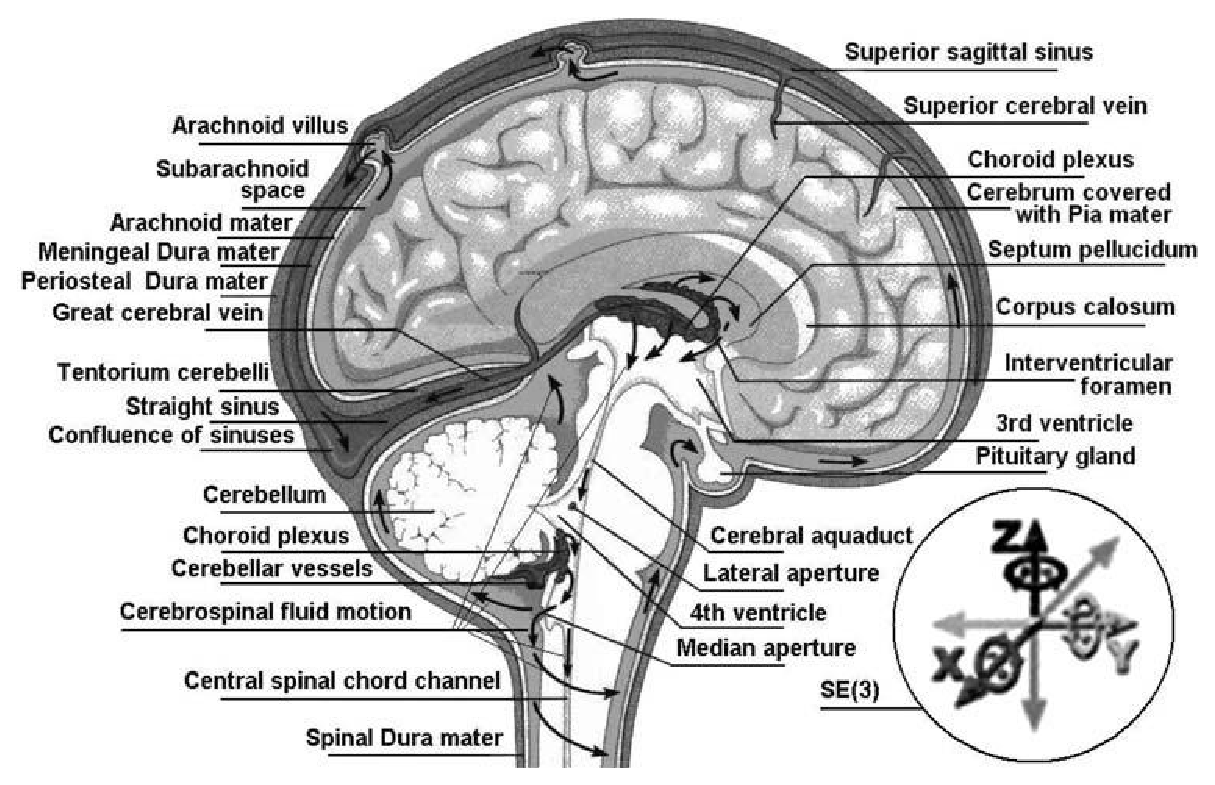
\includegraphics[width=13cm]{BrainInj}}
\caption{人脑和它的颅腔内脑脊液内的微观三维运动$SE(3)$群。}
\label{BrainInj}
\end{figure}


为了证明这一点,基于先前定义的协变力定律,我们首先建立了完全耦合的牛顿–欧拉动力学:

1.\quad 脑在颅腔内脑脊液中的微运动;

2.\quad 沿着脊柱的任何局部椎体间运动;以及

3.\quad 人体肌肉骨骼系统中的任何局部关节运动。\newline

然后,我们从中定义了\textbf{欧几里得震动(Euclidean Jolt)}的基本概念,这是所有机械损伤的主要原因。欧几里得震动有两个主要组成部分:

1.\quad 突然的运动,由意外的撞击或轻微扭曲的人体运动引起;以及

2.\quad 人体不自然的质量分布(可能有一些附加的质量),这会导致一些质量偏离自然生理的身体状态。
\begin{figure}[h]
\centerline{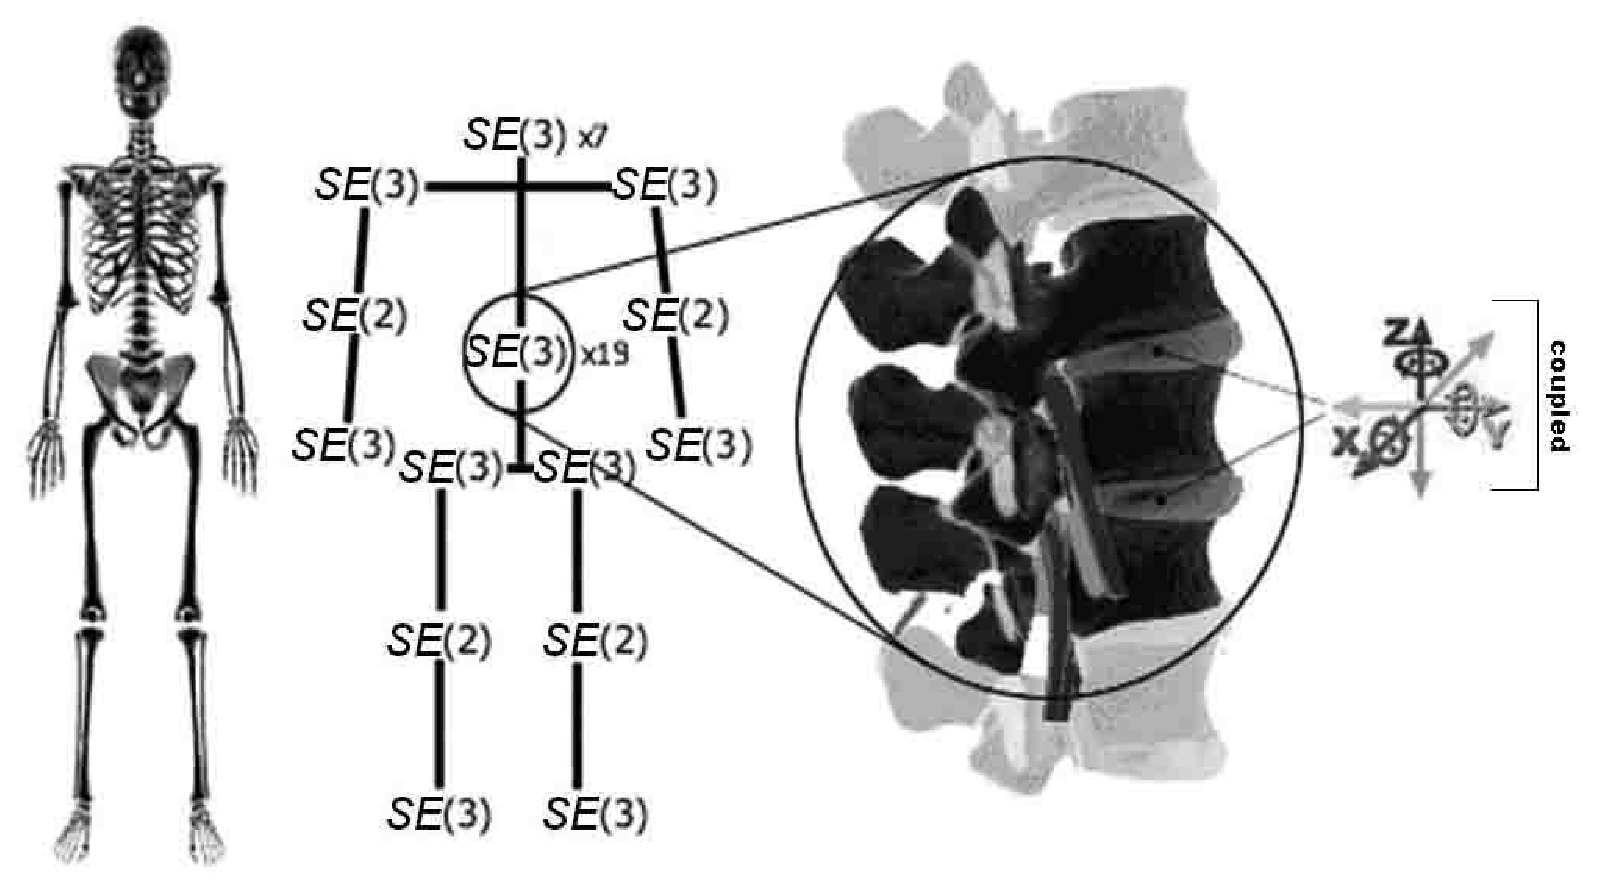
\includegraphics[width=13cm]{SpineSE3}}
\caption{以刚体运动的$SE(3)/SE(2)$群表示人体,其中脊柱表示为$26$个挠性耦合的$SE(3)$群的链。}
\label{SpineSE3}
\end{figure}

这一切意味着什么?我们将尝试用“简单英语”来解释。由于我们生活在一个三维空间中,人们可能会认为,人体的任何部分的运动,无论是由意外撞击还是由人类自愿运动引起的,“都只在6个自由度上遵循经典力学:三次平移和三次旋转”。然而,这6个自由度并不是标准术语“自由度”所暗示的独立运动。在现实中,空间中任何物体的这六种运动都是耦合的。首先,在所谓的旋转群(或矩阵,或四元数)中耦合三个旋转。其次,将三个平移与旋转群相结合,以给出空间中刚体运动的完整欧几里得群。看到这一点的一个简单方法是观察某人向空中投掷物体或击打网球:它将飞多远和飞到哪里不仅取决于标准的“抛射体”力学,还取决于它同时围绕所有三个轴的局部“自旋(spin)”。每个高尔夫和网球运动员都知道这个简单的事实。一旦正确定义了自旋,我们就有了“完全耦合的牛顿–欧拉动力学” -- 从这里开始。\newline

任何生物动力学系统的协变力定律(我们早些时候在我们的生物动力书籍和论文中介绍过,见我们在上面引用的论文中的参考资料)比牛顿–欧拉动力学更进了一步。它指出:
\begin{eqnarray*}
\mathbf{Euclidean\ Force\ covector\ field\ } \qquad\mathbf{=\newline
} \\
\mathbf{Body\ mass\ distribution\ \times \ Euclidean\ Acceleration\
vector\ field}
\end{eqnarray*}

这是对牛顿关于作用在单个粒子上的力的基本定义的一个非平凡的生物力学概括。与多体系统的经典工程力学不同,生物力学的这一基本定律提出,作用在多体系统上并导致其运动的力与由此产生的加速度是根本不同的物理量。简单地说,力是有质量的量,而加速度是无质量的量。更准确地说,加速度向量场包括各个身体节段的所有线性和角度加速度。当我们将它们与所有身体节段(包括所有质量和惯性矩)的总身体质量分布矩阵相耦合时,我们得到了力向量场,包括作用在各个身体节段上的所有力和力矩。通过这种方式,我们就为一个任意的生物力学系统定义了6维欧几里得力。
\begin{figure}[h]
\centerline{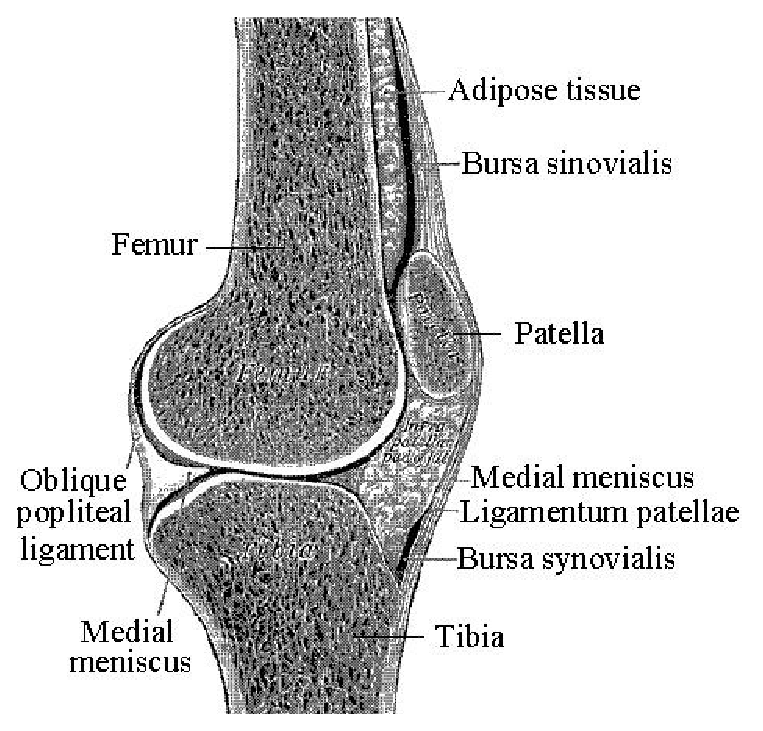
\includegraphics[width=7cm]{KneeInj}}
\caption{左膝关节的侧视正视图。尽管设计主要用于弯曲/伸展(严格地在矢状面上),但在半屈曲位置时有一些受限的内侧/外侧旋转,很明显膝关节确实有至少六个自由度,包括三个微平移。这种伤害实际上发生在某些微观翻译变得宏观时,通常只有在外部震动后才会发生。}
\label{KneeInj}
\end{figure}

现在,为了预测损伤,我们需要采用上述欧几里得生物力学的力的变化率(或相对于时间的导数)。通过这种方式,我们得到欧几里得震动,这是6维欧几里得力(在时间上)的突然变化:
\begin{eqnarray*}
\mathbf{Euclidean\ Jolt\ covector\ field\ } \qquad\mathbf{=\ } \\
\mathbf{Body\ mass\ distribution\ \times \ Euclidean\ Jerk\ vector\ field}
\end{eqnarray*}

同样,它由两个部分组成: (i) 无质量的线性和角度急动(所有包含的身体节段),以及 (ii) 它们的质量分布。为了简化,我们可以说质量分布矩阵包括所有涉及的节段的质量和惯性矩,以及来自正常生理状态的“偏心”或“病理杠杆”。\newline

因此,所有大脑、脊柱和肌肉骨骼损伤的唯一原因有两个部分:

1.\quad 耦合线性和角度急动;以及

2.\quad 具有“偏心”的质量分布。\newline

\noindent 换句话说,\textbf{在没有任何质量偏心的静态条件下就没有任何损伤;所有的损伤都是由相互耦合的线性和角度急动(jerk)引起的,这些急动也与所涉及的人体质量分布相耦合。}\newline


欧几里得震动导致两种形式的不连续的大脑、脊柱或肌肉骨骼损伤:

1.\quad 轻度旋转错向;以及

2.\quad 严重的平移错位(或骨折)。\newline

在上述引用的论文中,我们使用Cosserat多极粘弹性连续体模型,开发了由欧几里得震动引起的生物力学错向和错位的柔体动力学。\\

新的通用理论的含义是多方面的,如下所示。\newline

\noindent\textbf{A.} ~~创伤性脑损伤(TBI,参见图 \ref{BrainInj})的研究到目前为止已经确定,由于各种碰撞/撞击,脑干旋转是导致TBI的主要原因。我们的通用震动理论对TBI研究的贡献如下:\newline

1.\quad 严格地将这种大脑旋转定义为通过Cosserat多极柔体模型建模的脑干组织的机械错向;

2.\quad 表明大脑旋转从来不是单轴的,而总是三轴的;

3.\quad 表明大脑旋转总是伴随着平移错位。这是我们通用的震动理论的直接结果。\newline

这些看似“显而易见”的事实实际上是\textbf{全新的}:我们无法从平移中单独分析大脑的快速旋转,因为事实上它们总是耦合的。\newline

大脑震动理论的一个实际应用是头盔的设计。简言之,“硬”头盔可以拯救头骨,但不能拯救大脑;或者,“软”头盔可以保护大脑免受碰撞震动,但不能保护头骨。好的头盔既“硬”又“软”。一个合适的头盔需要有一个坚硬的外壳(保护头骨)和一个柔软的内部部分(这将通过自身的破坏来消散碰撞震动产生的能量,就像汽车通过自身的毁灭来保护乘客免受碰撞震动一样)。\newline

同样,在设计更安全的汽车安全气囊时,两个关键点将是 (i) 它们在汽车内的位置,以及 (ii) 它们的“软硬特性”,与上述头盔特性类似。\newline

\noindent\textbf{B.} ~~在脊柱损伤的情况下(参见图 \ref{SpineSE3}),我们通用的震动理论的贡献如下:\newline

1.\quad 脊柱损伤总是局限于某一椎体或椎间点;

2.\quad 在严重平移损伤(椎体骨折或盘状疝)的情况下,可以使用X射线或其它医学成像扫描进行识别;如果是显微旋转损伤(导致背痛综合征),则无法使用当前的医学成像扫描进行识别;

3.\quad 没有以下两种原因之一的脊柱损伤:

\qquad a.~~~由人体快速运动或各种碰撞/撞击引起的冲击性旋转 + 平移载荷;和/或

\qquad b.~~~由外部负荷引起的与正常生理脊柱形态的静态偏心;

\qquad c.~~~任何脊柱损伤都是由上述两点的组合造成的:冲击性旋转 + 平移负荷和静态偏心率。\newline

这是我们通用的震动理论的直接结果。我们不能单独分析平移和旋转的脊柱损伤。此外,没有偏心就没有“静态损伤”。几个世纪以来,印度妇女在头上背负着沉重的重物,没有任何脊椎损伤;她们只是防止了负载偏心和运动中的任何震动。\newline

目前使用的“主要负荷假设”以脊柱张力、压缩、弯曲和剪切来描述脊柱损伤,仅涵盖了我们通用的震动理论所涵盖的所有脊柱损伤的一小部分。为了防止脊柱损伤,我们需要发展脊柱震动意识:控制所有可能的冲击性脊柱负荷以及静态偏心的能力。%
\newline

\noindent\textbf{C.} ~~在一般肌肉骨骼损伤的情况下(膝盖损伤的具体情况见图 \ref{KneeInj}),我们通用的震动理论的贡献如下:\newline

1.\quad 损伤总是局限于某个关节或骨骼,并由同时以多个耦合自由度撞击该特定关节/骨骼的脉冲负载引起;

2.\quad 当大部分身体质量悬挂在该关节上时,会发生损伤;例如,在膝盖受伤的情况下,当大部分身体质量压在一条腿上,膝盖半弯曲时,然后,由于一些外部冲击,膝盖突然“急动” (这可能发生在跑步、滑雪和球类运动中,以及各种碰撞/撞击中);或者,在肩部受伤的情况下,当大部分身体质量挂在一只手臂上,然后突然急动。\newline

为了防止这些损伤,我们需要发展肌肉骨骼震动意识。例如,切勿使弯曲的膝盖过载,避免任何不受控制的运动(如滑倒)或与外部物体碰撞。

\subsection{创伤性脑损伤(TBI)的分析力学}

\subsubsection{$SE(3)$震动:TBI的原因}

在本小节中,我们简要介绍TBI力学。有关更多详细信息和参考文献,参见文献 \cite{ivbrain}。

在现代动力学的语言中,人脑在颅内内的微观运动,由3D运动的欧几里得$SE(3)$群(见下一小节)控制。在大脑的$SE(3)$群中,我们既有$SE(3)$运动学(由$SE(3)$速度及其两个时间导数组成:$SE(3)$加速度和$SE(3)$急动度(jerk)),也有$SE(3)$动力学(包括$SE(3)$动量及其两个时间导数:$SE(3)$力和$SE(3)$)震动(jolt)),这是大脑的运动学 $\times$ 大脑的质量–惯性分布。

非正式地说,外部$SE(3)$震动\footnote{机械$SE(3)$震动概念基于更高阶相切(tangency)的数学概念(在头部的构型流形的射流丛(jet bundle)中严格定义),如下所示:当物体撞击人类头部或头部撞击外部物体时,我们会发生碰撞。这自然由$SE(3)$动量来描述,它是3个线性牛顿动量与3个角度欧拉动量的非线性耦合。$SE(3)$动量的相切,由(绝对的)时间导数定义,是$SE(3)$力。二阶相切由$SE(3)$震动给出,它是$SE(3)$力的相切,也由时间导数定义。}是作用于大脑质量–惯性分布(由大脑质量和惯性矩阵给出)的$SE(3)$力的急剧和突然变化。也就是说,一个3D力向量的“增量”变化与一个3D扭矩向量耦合,在大脑浸入脑脊液的情况下撞击头部外壳。换句话说,$SE(3)$震动是大脑在脑脊液中连续微运动的所有6个耦合维度上,即在三个笛卡尔($x,y,z$)平移和围绕笛卡尔轴的三个对应的欧拉角内:横滚、俯仰和偏航,突然、剧烈和不连续的冲击(图 \ref{BrainInj})。如果$SE(3)$震动对大脑产生轻微的冲击(例如强烈的头部震动),则会导致轻度TBI,相关的感觉运动和/或认知功能暂时丧失,呼吸和运动受到影响。如果$SE(3)$震动产生强烈的冲击(用外部质量撞击头部),则会导致严重的TBI,完全丧失手势、言语和动作。

$SE(3)$震动是协变力1–形式(或,协向量场)的绝对时间导数。生物力学的基本定律是协变力定律(\emph{covariant force law}):
$$\text{Force co-vector field}=\text{Mass distribution}\times \text{%
Acceleration vector--field},$$ 其被正式写为(使用爱因斯坦求和惯例,索引标记三个笛卡尔平移和三个对应的欧拉角):
\begin{equation*}
F_{{\mu}}=m_{{\mu}{\nu}}a^{{\nu}},\qquad ({\mu,\nu}%
=1,...,6)
\end{equation*}
其中,$F_{{\mu}}$表示外部“推动”$SE(3)$力协向量场的6个协变分量,$m_{{\mu}{\nu}}$表示大脑惯性–度量张量的6$\times $6个协变量分量,而$a^{{\nu}}$对应于大脑内部$SE(3)$加速度向量场的6个逆变分量。

现在,协变$SE(3)$力 $F_{{\mu }}$ 的协变(绝对的,Bianchi)时间导数 $\frac{{D}}{dt}(\cdot )$ 定义了相应的外部“打击”$SE(3)$震动协向量场:
\begin{equation}
\frac{{D}}{dt}(F_{{\mu }})=m_{{\mu }{\nu }}\frac{{D}}{dt}(a^{{\nu }})=m_{{%
\mu }{\nu }}\left( \dot{a}^{{\nu }}+\Gamma _{\mu \lambda }^{{\nu }}a^{{\mu }%
}a^{{\lambda }}\right) ,  \label{Bianchi}
\end{equation}%
其中 ${\frac{{D}}{dt}}{(}a^{{\nu }})$ 表示大脑内部$SE(3)$急动度向量场的6个逆变分量,而上标点 ($\dot{~}$) 表示时间导数。$\Gamma _{\mu \lambda }^{{\nu }}$ 是$SE(3)$群的Levi–Civita连通的Christoffel符号,其在纯笛卡尔平移情况下为零,在旋转以及平移和旋转的完全耦合情况下为非零。

在下文中,我们详细阐述$SE(3)$震动概念(使用向量和张量方法),及其以大脑错位和错向的形式产生的生物物理TBI后果。

\subsubsection{在脑脊液中的大脑微运动$SE(3)$群}

在正常心率的频率范围内,大脑和脑脊液以脉动的方式共同表现出周期性的微观平移和旋转运动(伴随着脑室的周期性挤压)。这种微运动在数学上由欧几里得(度量) $SE(3)$ 群定义。

换言之,浸入颅腔内脑脊液中的大脑的欧几里得微运动的规范 $SE(3)$ 群包含形式 {\small $ \left(
\begin{array}{cc}
{\bf R} & {\bf b} \\
0 & 1
\end{array}
\right)$}的矩阵,其中${\bf b}$是大脑的3D微平移向量,并且${\bf R}$ 是大脑的3D旋转矩阵,由大脑的三个欧拉微旋转的乘积${\bf R}=R_{\varphi }\cdot R_{\psi }\cdot R_{\theta }$给出,$\text{roll}=R_{\varphi },~\text{pitch}=R_{\psi },~\text{yaw}=R_{\theta }$,分别围绕$x$轴以角度$ \varphi $、围绕$y$轴以角度$\psi$和围绕$z$轴以角度$\theta $执行旋转,
{\small
\begin{equation*}
R_{\varphi } =\left[
\begin{array}{ccc}
1 & 0 & 0 \\
0 & \cos \varphi & -\sin \varphi \\
0 & \sin \varphi & \cos \varphi%
\end{array}
\right] , ~~ R_{\psi } =\left[
\begin{array}{ccc}
\cos \psi & 0 & \sin \psi \\
0 & 1 & 0 \\
-\sin \psi & 0 & \cos \psi%
\end{array}
\right] , ~~ R_{\theta } =\left[
\begin{array}{ccc}
\cos \theta & -\sin \theta & 0 \\
\sin \theta & \cos \theta & 0 \\
0 & 0 & 1%
\end{array}
\right].
\end{equation*}}

因此,大脑在脑脊液中的自然 $SE(3)$ 动力学由牛顿(平移)和欧拉(旋转)微运动方程的耦合给出。


\subsubsection{大脑的自然 $SE(3)$ 动力学}

为了支持我们的耦合负载速率假设,我们在头骨的$SE(3)$运动群中建立了大脑微运动的耦合牛顿−欧拉动力学。力的牛顿−欧拉方程以向量(粗体)形式读取为
\begin{eqnarray}
\text{Newton} &:&~\boldsymbol{\dot{\mathbf p}}~\boldsymbol{\equiv \mathbf M\dot{\mathbf v}=\mathbf{F+p}\times \omega }%
,  \label{vecForm} \\
\text{Euler} &:&~\boldsymbol{\dot{\pi}}~\boldsymbol{\equiv \mathbf I\dot{\omega}=\mathbf T+\pi
\times \omega +\mathbf p\times \mathbf v},  \notag
\end{eqnarray}
其中$\times $ 表示向量叉积,\footnote{回想一下,两个向量$\mathbf{u} $和$\mathbf{v}$的叉积$\mathbf{u\times v}$等于$\mathbf{u\times v}=uv\func{sin}\theta \mathbf{n}$,其中$\theta $是$\mathbf{u} $和$\mathbf{v}$之间的角度,而$ \mathbf{n}$是垂直于$\mathbf{u} $和$\mathbf{v}$平面的单位向量,因此$\mathbf{u} $和$\mathbf{v}$形成右手系统。}
\begin{equation*}
\mathbf{M}\equiv M_{ij}=diag\{m_{1},m_{2},m_{3}\}\qquad \text{and}\qquad
\mathbf{I}\equiv I_{ij}=diag\{I_{1},I_{2},I_{3}\},\qquad(i,j=1,2,3)
\end{equation*}
是大脑的(对角)质量和惯性矩阵,\footnote{实际上,质量和惯性矩阵($\mathbf{M,I}$)不是对角的,而是完整的$3\times 3$正定对称矩阵,具有耦合的质量和惯性乘积。更现实的是,浸没在(不可压缩的、非旋转的和非粘性的)脑脊液中的大脑的完全耦合质量–惯性特性单一的非对角线的$6\times 6$正定对称质量–惯性矩阵$ \mathcal{M}_{SE(3)}$定义,即$SE(3)$群的所谓原料度量张量,它具有所有非零质量–惯性耦合乘积。换句话说,$6\times 6$矩阵$\mathcal{M}_{SE(3)}$包含: (i) 大脑自身质量加上与液体相关的附加质量矩阵, (ii) 大脑自身惯性加上与液体潜在流量相关的附加惯性矩阵,以及 (iii) 线性动量和角度动量之间的所有耦合项。然而,为了简单起见,在本文中,我们将只考虑两个独立的对角$3\times 3$矩阵($\mathbf{M,I}$)的简单情况。}定义了大脑的质量–惯性分布,其主要惯性矩在笛卡尔坐标($x,y,z$)中通过体积积分给出
\begin{equation*}
I_{1}=\iiint \rho (z^{2}+y^{2})dxdydz,~~I_{2}=\iiint \rho
(x^{2}+z^{2})dxdydz,~~I_{3}=\iiint \rho (x^{2}+y^{2})dxdydz,
\end{equation*}
这取决于大脑密度$\rho =\rho (x,y,z)$,
\begin{equation*}
\mathbf{v}\equiv v^{i}=[v_{1},v_{2},v_{3}]^{t}\qquad \text{and\qquad }%
\mathbf{\omega }\equiv {\omega }^{i}=[\omega _{1},\omega _{2},\omega
_{3}]^{t}
\end{equation*}
(其中$[~]^{t}$表示向量转置)是大脑的线性和角度速度向量\footnote{实际上,$\mathbf{\omega }$是一个$3\times 3$的姿态矩阵(\emph{attitude matrix})。然而,为了简单起见,我们将坚持(大部分)对称的平移-旋转向量形式。}(即列向量),
\begin{equation*}
\mathbf{F}\equiv F_{i}=[F_{1},F_{2},F_{3}]\qquad \text{and}\qquad \mathbf{T}%
\equiv T_{i}=[T_{1},T_{2},T_{3}]
\end{equation*}
是作用在头骨内的大脑上的重力和其它外力和扭矩协向量(即行向量),
\begin{eqnarray*}
\mathbf{p} &\equiv &p_{i}\equiv \mathbf{Mv}%
=[p_{1},p_{2},p_{3}]=[m_{1}v_{1},m_{2}v_{2},m_{2}v_{2}]\qquad \text{and} \\
\mathbf{\pi } &\equiv &\pi _{i}\equiv \mathbf{I\omega }=[\pi _{1},\pi
_{2},\pi _{3}]=[I_{1}\omega _{1},I_{2}\omega _{2},I_{3}\omega _{3}]
\end{eqnarray*}
是大脑的线性和角动量协向量。

在张量形式中,力的牛顿-欧拉方程(\ref{vecForm})读取为
\begin{eqnarray*}
\dot{p}_{i} &\equiv &M_{ij}\dot{v}^{j}=F_{i}+\varepsilon _{ik}^{j}p_{j}{%
\omega }^{k},\qquad(i,j,k=1,2,3) \\
\dot{\pi}_{i} &\equiv &I_{ij}\dot{\omega}^{j}=T_{i}+\varepsilon _{ik}^{j}\pi
_{j}\omega ^{k}+\varepsilon _{ik}^{j}p_{j}v^{k},
\end{eqnarray*}
其中置换符号$\varepsilon _{ik}^{j}$定义为
\begin{equation*}
\varepsilon _{ik}^{j}=
\begin{cases}
+1 & \text{if }(i,j,k)\text{ is }(1,2,3),(3,1,2)\text{ or }(2,3,1), \\
-1 & \text{if }(i,j,k)\text{ is }(3,2,1),(1,3,2)\text{ or }(2,1,3), \\
0 & \text{otherwise: }i=j\text{ or }j=k\text{ or }k=i.
\end{cases}
\end{equation*}

在标量形式中,力的牛顿-欧拉方程(\ref{vecForm})展开为
\begin{eqnarray}
\text{Newton} &:&\left\{
\begin{array}{c}
\dot{p}_{_{1}}={F_{1}}-{m_{3}}{v_{3}}{\omega _{2}}+{m_{2}}{v_{2}}{\omega _{3}%
} \\
\dot{p}_{_{2}}={F_{2}}+{m_{3}}{v_{3}}{\omega _{1}}-{m_{1}}{v_{1}}{\omega _{3}%
} \\
\dot{p}_{_{3}}={F_{3}}-{m_{2}}{v_{2}}{\omega _{1}}+{m_{1}}{v_{1}}{\omega _{2}%
}
\end{array}
\right. ,  \label{scalarForm} \\
\text{Euler} &:&\left\{
\begin{array}{c}
\dot{\pi}_{_{1}}={T_{1}}+({m_{2}}-{m_{3}}){v_{2}}{v_{3}}+({I_{2}}-{I_{3}}){%
\omega _{2}}{\omega _{3}} \\
\dot{\pi}_{_{2}}={T_{2}}+({m_{3}}-{m_{1}}){v_{1}}{v_{3}}+({I_{3}}-{I_{1}}){%
\omega _{1}}{\omega _{3}} \\
\dot{\pi}_{_{3}}={T_{3}}+({m_{1}}-{m_{2}}){v_{1}}{v_{2}}+({I_{1}}-{I_{2}}){%
\omega _{1}}{\omega _{2}}
\end{array}
\right. ,  \notag
\end{eqnarray}
这显示了大脑的个体质量和惯性的耦合。

方程(\ref{vecForm})–(\ref{scalarForm})可以从大脑的平移 + 旋转动能推导出来\footnote{%
在完全耦合的牛顿 -- 欧拉大脑动力学中,代替方程(\ref {Ek}),我们将用内积来定义大脑的动能:
\begin{equation*}
E_{k}=\frac{1}{2}\left[ \QOVERD( ) {\mathbf{p}}{\mathbf{\pi }}\left|
\mathcal{M}_{SE(3)}\right. \QOVERD( ) {\mathbf{p}}{\mathbf{\pi }}\right] .
\end{equation*}
}
\begin{equation}
E_{k}={\frac{1}{2}}\mathbf{v}^{t}\mathbf{Mv}+{\frac{1}{2}}\mathbf{\omega }%
^{t}\mathbf{I\omega },  \label{Ek}
\end{equation}
或,以张量形式
\begin{equation*}
E={\frac{1}{2}}M_{ij}{v}^{i}{v}^{j}+{\frac{1}{2}}I_{ij}{\omega}%
^{i}{\omega}^{j}.
\end{equation*}

为此,我们使用基尔霍夫 -- 拉格朗日方程(\emph{Kirchhoff--Lagrangian equations}):
\begin{eqnarray}
\frac{d}{{dt}}\partial _{\mathbf{v}}E_{k} &=&\partial _{\mathbf{v}%
}E_{k}\times \mathbf{\omega }+\mathbf{F},  \label{Kirch} \\
{\frac{d}{{dt}}}\partial _{\mathbf{\omega }}E_{k} &=&\partial _{\mathbf{%
\omega }}E_{k}\times \mathbf{\omega }+\partial _{\mathbf{v}}E_{k}\times
\mathbf{v}+\mathbf{T},  \notag
\end{eqnarray}
其中 $\partial _{\mathbf{v}}E_{k}=\frac{\partial E_{k}}{\partial \mathbf{v}}%
,~\partial _{\mathbf{\omega }}E_{k}=\frac{\partial E_{k}}{\partial \mathbf{%
\omega }}$;这些方程以张量形式读取为
\begin{eqnarray*}
\frac{d}{dt}\partial _{v^{i}}E &=&\varepsilon _{ik}^{j}\left( \partial
_{v^{j}}E\right) \omega ^{k}+F_{i}, \\
\frac{d}{dt}\partial _{{\omega }^{i}}E &=&\varepsilon _{ik}^{j}\left(
\partial _{{\omega }^{j}}E\right) {\omega }^{k}+\varepsilon _{ik}^{j}\left(
\partial _{v^{j}}E\right) v^{k}+T_{i}.
\end{eqnarray*}

使用方程(\ref{Ek})--(\ref{Kirch}),大脑的线性和角动量协向量定义为
\begin{equation*}
\mathbf{p}=\partial _{\mathbf{v}}E_{k}{,\qquad \mathbf{\pi }=\partial _{%
\mathbf{\omega }}E_{k},}
\end{equation*}
或,以张量形式
\begin{equation*}
p_{i}=\partial _{v^{i}}E{,\qquad }\pi _{i}=\partial _{{\omega }^{i}}E,
\end{equation*}
及其相应的时间导数,以向量形式
\begin{equation*}
~\boldsymbol{\dot{\mathbf p}}=\frac{d}{dt}\mathbf{p=}\frac{d}{dt}\partial _{\mathbf{v}}E{%
,\qquad \boldsymbol{\dot{\pi}}=}\frac{d}{dt}\mathbf{\pi =}\frac{d}{dt}\partial _{%
\mathbf{\omega }}E,
\end{equation*}
或,以张量形式
\begin{equation*}
~\dot{p}_{i}=\frac{d}{dt}p_{i}=\frac{d}{dt}\partial _{v^{i}}E{,\qquad \dot{%
\pi}_{i}=}\frac{d}{dt}\pi _{i}=\frac{d}{dt}\partial _{{\omega }^{i}}E,
\end{equation*}
或,以标量形式
\begin{equation*}
\boldsymbol{\dot{\mathbf p}}=[\dot{p}_{1},\dot{p}_{2},\dot{p}_{3}]=[m_{1}\dot{v}%
_{1},m_{2}\dot{v}_{2},m_{3}\dot{v}_{3}],\qquad {\boldsymbol{\dot{\pi}}}=[\dot{\pi%
}_{1},\dot{\pi}_{2},\dot{\pi}_{3}]=[I_{1}\dot{\omega}_{1},I_{2}\dot{\omega}%
_{2},I_{3}\dot{\omega}_{3}].
\end{equation*}

虽然脑脊髓液中健康的$SE(3)$动力学由耦合的牛顿−欧拉微动力学给出,但TBI实际上是由这种自然$SE(3)$微动力学中的剧烈和不连续变化引起的,以$SE(3)$震动的形式,导致大脑的不连续变形。


\subsubsection{大脑的创伤动力学:$SE(3)$震动}

$SE(3)$震动,即TBI的实际原因(以大脑的塑性变形的形式),被定义为牛顿 + 欧拉的耦合震动;在(协)向量形式中,$SE(3)$震动读取为\footnote{%
注意,两个向量的叉积的导数遵循标准微积分积规则: $\frac{d}{dt}(\mathbf{u\times v})=\dot{\mathbf{u}}\times \mathbf{v}+\mathbf{u}\times \dot{\mathbf{v}}.$}
\begin{equation*}
SE(3)-\text{jolt}:\left\{
\begin{array}{l}
\text{Newton~jolt}:\boldsymbol{\dot{\mathbf F}=\ddot{\mathbf p}-\dot{\mathbf p}\times \omega -\mathbf p\times
\dot{\omega}}~,\qquad \\
\text{Euler~jolt}:\boldsymbol{\dot{\mathbf T}=\ddot{\pi}}~\boldsymbol{-\dot{\pi}\times
\omega -\pi \times \dot{\omega}-\dot{\mathbf p}\times \mathbf v-\mathbf p\times \dot{\mathbf v}},
\end{array}
\right.
\end{equation*}
其中,线性和角度震动协向量为
\begin{equation*}
\boldsymbol{\dot{\mathbf F}\equiv \mathbf M\ddot{\mathbf v}}=[\dot{F}_{{1}},\dot{F}_{{2}},\dot{F}_{{3}%
}],\qquad \boldsymbol{\dot{\mathbf T}\equiv \mathbf I\ddot{\omega}}=[\dot{T}_{{1}},\dot{T}_{{2}},%
\dot{T}_{{3}}],
\end{equation*}
其中
\begin{equation*}
\boldsymbol{\ddot{\mathbf v}}=[\ddot{v}_{{1}},\ddot{v}_{{2}},\ddot{v}_{{3}}]^{t},\qquad
\boldsymbol{\ddot{\omega}}=[\ddot{\omega}_{{1}},\ddot{\omega}_{{2}},\ddot{\omega}%
_{{3}}]^{t},
\end{equation*}
是线性和角度急动度向量。

在张量形式中,$SE(3)$震动读取为\footnote{%
在本段中,上标点实际上表示绝对Bianchi (协变)时间导数方程(\ref{Bianchi}),因此震动保持正确的协向量特征,如果使用普通时间导数,则会丢失该特征。然而,为了简单和更广泛的可读性,我们坚持使用相同的上标点符号。}
\begin{eqnarray*}
~\dot{F}_{i} &=&\ddot{p}_{i}-\varepsilon _{ik}^{j}\dot{p}_{j}{\omega }%
^{k}-\varepsilon _{ik}^{j}p_{j}{\dot{\omega}}^{k}, \qquad(i,j,k=1,2,3) \\
~\dot{T}_{{i}} &=&\ddot{\pi}_{i}~-\varepsilon _{ik}^{j}\dot{\pi}_{j}\omega
^{k}-\varepsilon _{ik}^{j}\pi _{j}{\dot{\omega}}^{k}-\varepsilon _{ik}^{j}%
\dot{p}_{j}v^{k}-\varepsilon _{ik}^{j}p_{j}\dot{v}^{k},
\end{eqnarray*}
其中,线性和角度震动协向量定义为
\begin{eqnarray*}
\boldsymbol{\dot{\mathbf F}} &\equiv &\dot{F}_{i}=\boldsymbol{\mathbf M\ddot{\mathbf v}}\,\equiv \mathbf{\,}%
M_{ij}\ddot{v}^{j}=[\dot{F}_{1},\dot{F}_{2},\dot{F}_{3}], \\
\boldsymbol{\dot{\mathbf T}} &\equiv &\dot{T}_{{i}}=\boldsymbol{\mathbf I\ddot{\omega}\equiv \,}%
I_{ij}\ddot{\omega}^{j}=[\dot{T}_{{1}},\dot{T}_{{2}},\dot{T}_{{3}}],
\end{eqnarray*}
其中 $\mathbf{\ddot{v}}=\ddot{v}^{{i}}$,以及 $\mathbf{\ddot{\omega}}=%
\ddot{\omega}^{{i}}$ 是线性和角度急动度向量。

在标量形式中,$SE(3)$震动展开为
\begin{eqnarray*}
\text{Newton~jolt} &:&\left\{
\begin{array}{l}
\dot{F}_{{1}}=\ddot{p}_{1}-m_{{2}}\omega _{{3}}\dot{v}_{{2}}+m_{{3}}\left( {%
\omega }_{{2}}\dot{v}_{{3}}+v_{{3}}\dot{\omega}_{{2}}\right) -m_{{2}}v_{{2}}{%
\dot{\omega}}_{{3}}, \\
\dot{F}_{{2}}=\ddot{p}_{2}+m_{{1}}\omega _{{3}}\dot{v}_{{1}}-m_{{3}}\omega _{%
{1}}\dot{v}_{{3}}-m_{{3}}v_{{3}}\dot{\omega}_{{1}}+m_{{1}}v_{{1}}\dot{\omega}%
_{{3}}, \\
\dot{F}_{{3}}=\ddot{p}_{3}-m_{{1}}\omega _{{2}}\dot{v}_{{1}}+m_{{2}}\omega _{%
{1}}\dot{v}_{{2}}-v_{{2}}\dot{\omega}_{{1}}-m_{{1}}v_{{1}}\dot{\omega}_{{2}},
\end{array}
\right. \\
&& \\
\text{Euler~jolt} &:&\left\{
\begin{array}{l}
\dot{T}_{{1}}=\ddot{\pi}_{1}-(m_{{2}}-m_{{3}})\left( v_{{3}}\dot{v}_{{2}}+v_{%
{2}}\dot{v}_{{3}}\right) -(I_{{2}}-I_{{3}})\left( \omega _{{3}}\dot{\omega}_{%
{2}}+{\omega }_{{2}}{\dot{\omega}}_{{3}}\right) , \\
\dot{T}_{{2}}=\ddot{\pi}_{2}+(m_{{1}}-m_{{3}})\left( v_{{3}}\dot{v}_{{1}}+v_{%
{1}}\dot{v}_{{3}}\right) +(I_{{1}}-I_{{3}})\left( {\omega }_{{3}}{\dot{\omega%
}}_{{1}}+{\omega }_{{1}}{\dot{\omega}}_{{3}}\right) , \\
\dot{T}_{{3}}=\ddot{\pi}_{3}-(m_{{1}}-m_{{2}})\left( v_{{2}}\dot{v}_{{1}}+v_{%
{1}}\dot{v}_{{2}}\right) -(I_{{1}}-I_{{2}})\left( {\omega }_{{2}}{\dot{\omega%
}}_{{1}}+{\omega }_{{1}}{\dot{\omega}}_{{2}}\right).
\end{array}
\right.
\end{eqnarray*}

我们在此指出,线性和角动量($\mathbf{p,\pi }$)、力($\mathbf{F,T}$)和震动($\boldsymbol{\dot{\mathbf F},\dot{\mathbf T}}$)是协向量(行向量),而线速度和角速度($\mathbf{ v,\omega }$)、加速度($\boldsymbol{\dot{\mathbf v},\dot{\omega}}$)和急动度($ \boldsymbol{\ddot{\mathbf v},\ddot{\omega}}$)是向量(列向量)。这在生物物理意义上意味着,“急动”向量不应与“震动”协向量混淆。例如,“急动”意味着晃动头部自身的质量惯性矩阵(主要是寰枕关节和寰枢关节),而“震动”则意味着实际用一些外部质量惯性矩阵撞击头部,包括在“撞击”$SE(3)$震动中的,或者用头部撞击一些外部静止/大质量的物体(例如,地面–重力效应或墙壁–惯性效应)。因此,无质量的“急动”向量表示(平移+旋转)非碰撞效应(\textit{non-collision effect}),只会导致较弱的脑损伤,而惯性“震动”协向量表示(平移+旋转)碰撞效应(\textit{collision effect}),会导致严重的脑损伤。

\subsubsection{$SE(3)$震动引起的大脑错位和错向}

从介绍中回想一下,对于轻度TBI,最好的损伤预测器被认为是大脑应变和应变率的乘积,这是标准的各向同性粘弹性连续体概念。为了改进这一标准概念,在本小节中,我们将人脑视为3D各向异性多极Cosserat粘弹性连续体(\emph{Cosserat viscoelastic continuum}),表现出耦合–应力–应变弹性特性。该非标准连续体模型适用于分析具有微观结构的多层材料中的塑性(不可逆)变形和断裂力学(其中的层的滑移和弯曲引入了额外的自由度,在标准连续体模型中不存在)。

$SE(3)$震动$(\boldsymbol{\dot{\mathbf F},\dot{\mathbf T}})$导致两种类型的大脑快速不连续变形:

\begin{enumerate}
\item  牛顿震动$\boldsymbol{\dot{\mathbf F}}$可导以致微平移错位(\emph{dislocations})或Cosserat平移中的不连续;

\item  欧拉震动$\boldsymbol{\dot{\mathbf T}}$可以导致微旋转错向(\emph{disclinations})或Cosserat旋转中的不连续。
\end{enumerate}

为精确定义$SE(3)$震动引起的大脑错位和错向$(\boldsymbol{\dot{\mathbf F},\dot{\mathbf T}})$, 我们首先定义坐标协帧(coordinate co-frame),即基的1-形式$\{dx^{i}\}$的集合,以局部坐标$x^{i}=(x^{1},x^{2},x^{3})=(x,y,z)$给出,附着到大脑的质心。然后,在坐标协帧$\{dx^{i}\}$中,我们引入了以下一组与大脑塑性变形相关的基于$SE(3)$的微分$p$-形式\footnote{%
微分$p$-形式是完全斜对称协变张量,使用外楔积和外导数定义。在光滑流形$M$上$p$-形式$\beta $的外导数$d$的正确定义包括庞加莱引理(\textit{Poincar\'{e} lemma}):{$d(d\beta )=0$},并验证了一般斯托克斯公式(\textit{general Stokes formula})
\[
\int_{\partial M}\beta =\int_{M}d\beta ,
\]
其中$M$是一个$p$维具有边界的流形(\emph{manifold with a boundary}),并且$\partial M$是其$(p-1)$维边界(\emph{boundary}),而积分具有适当的维数。
\par
如果一个$p$-形式$\beta $的外导数等于零,则称其为封闭的(\emph{closed}),
\[
d\beta =0.
\]
从这个条件可以看出,封闭形式(外导数算子$d$的核(\emph{kernel}))是守恒量。因此,封闭$p$-形式具有某些不变的性质,在物理上对应于守恒定律。
\par
一个$p$-形式$\beta $是某些$(p-1)$-形式$ \alpha $的外导数,
\[
\beta =d\alpha ,
\]
被称为是精确的(\emph{exact}) (外导数算子$d$的象(\emph{image}))。通过庞加莱引理(\textit{Poincar\'{e} lemma}),精确形式证明是自动封闭的,
\[
d\beta =d(d\alpha )=0.
\]
该引理是 de Rham 同调理论的基础。}:\newline\\
$~~~~$错位电流(\emph{dislocation current }) 1-形式,$\mathbf{J}=J_{i}\,dx^{i}$;%
\newline
$~~~~$错位密度(\emph{dislocation density }) 2-形式,$\mathbf{\alpha }=\frac{1}{2} \alpha _{ij}\,dx^{i}\wedge dx^{j}$;\newline
$~~~~$错向电流(\emph{disclination current }) 2-形式,$\mathbf{S}=\frac{1}{2} S_{ij}\,dx^{i}\wedge dx^{j}$;以及\newline
$~~~~$错向密度(\emph{disclination density }) 3-形式,$\mathbf{Q}=\frac{1}{3!} Q_{ijk}\,dx^{i}\wedge dx^{j}\wedge dx^{k}$,\newline
其中$\wedge $ 表示外部楔积(wedge--product)。这四种基于$SE(3)$的微分形式满足以下连续性方程组:
\begin{eqnarray}
&&\boldsymbol{\dot{\alpha}}=\mathbf{-dJ-S,}  \label{dis1} \\
&&\boldsymbol{\dot{\mathbf Q}}=\mathbf{-dS,}  \label{dis2} \\
&&\mathbf{d\alpha }=\mathbf{Q,}  \label{dis3} \\
&&\mathbf{dQ}=\mathbf{0,}\qquad   \label{dis4}
\end{eqnarray}
其中$\mathbf{d}$表示外导数。

在这方程组中,最简单的第四个方程(\ref{dis4}),表示比安基恒等式(\emph{Bianchi identity}),可被改写为
\[
\mathbf{dQ}=\partial _{l}Q_{[ijk]}\,dx^{l}\wedge dx^{i}\wedge
dx^{j}\wedge dx^{k}=0,
\]
其中,$\partial _{i}\equiv\partial /\partial x^{i}$,而$\theta _{\lbrack ij...]}$表示$\theta _{ij...}$的斜对称部分。

类似地,方程组中的第三个方程(\ref{dis3})读为
\begin{eqnarray*}
\frac{1}{3!}Q_{ijk}\,dx^{i}\wedge dx^{j}\wedge dx^{k} &=&\partial
_{k}\alpha
_{\lbrack ij]}\,dx^{k}\wedge dx^{i}\wedge dx^{j},\text{\qquad or} \\
Q_{ijk} &=&-6\partial _{k}\alpha _{\lbrack ij]}.
\end{eqnarray*}

方程组中的第二个方程(\ref{dis2})读为
\begin{eqnarray*}
\frac{1}{3!}\dot{Q}_{ijk}\,dx^{i}\wedge dx^{j}\wedge dx^{k}
&=&-\partial
_{k}S_{[ij]}\,dx^{k}\wedge dx^{i}\wedge dx^{j},\text{\qquad or} \\
\dot{Q}_{ijk} &=&6\partial _{k}S_{[ij]}.
\end{eqnarray*}

最后,方程组中的第一个方程(\ref{dis1})读为
\begin{eqnarray*}
\frac{1}{2}\dot{\alpha}_{ij}\,dx^{i}\wedge dx^{j} &=&(\partial _{j}J_{i}-%
\frac{1}{2}S_{ij})\,dx^{i}\wedge dx^{j},\text{\qquad or} \\
\dot{\alpha}_{ij}\, &=&2\partial _{j}J_{i}-S_{ij}\,.
\end{eqnarray*}

换句话说,我们有:

\begin{itemize}
\item  2-形式方程(\ref{dis1})将错位密度$\mathbf{\alpha }$的时间导数$\boldsymbol{\dot{\alpha}=}\frac{1}{2}\dot{\alpha}_{ij}\,dx^{i}\wedge dx^{j}$定义为错向电流$\mathbf{S}$和位错电流$\mathbf{J}$的旋度的(负)加和。

\item  3-形式方程(\ref{dis2})表明,错向密度$\mathbf{Q}$的时间导数$\boldsymbol{\dot{\mathbf Q}=}\frac{1}{3!}\dot{Q}_{ijk}\,dx^{i}\wedge dx^{j}\wedge dx^{k}$是错向电流$\mathbf{S}$的(负)散度。

\item  3-形式方程(\ref{dis3})将错向密度$\mathbf{Q}$定义为错位密度$\mathbf{\alpha }$的散度,即$\mathbf{Q}$是精确的(\emph{exact}) 3-形式。

\item  比安基恒等式方程(\ref{dis4})由庞加莱引理(\textit{Poincar\'{e} lemma})从方程(\ref{dis3})得出,并指出错向密度$\mathbf{Q}$是守恒量,即$\mathbf{Q}$是封闭的(\emph{closed}) 3-形式。此外,在3D空间中的每个4-形式都为零。
\end{itemize}

从这些方程中,我们可以推导出两个重要结论:

\begin{enumerate}
\item  作为错位的导数,大脑的错向是更高阶的张量,并因此是更复杂的量,这意味着它们比错位具有更高的严重TBI风险,这一事实\textbf{得到}文献的支持(参见文献\cite{ivbrain}引言中对现有TBI模型的回顾)。

\item  大脑的错位和错向由底层$SE(3)$群相互耦合,这意味着我们不能单独分析平移和旋转的TBI — 这一事实\textbf{没有得到}文献的支持。
\end{enumerate}

有关更多医疗细节和参考文献,参见文献\cite{ivbrain}。


\begin{thebibliography}{99}
\bibitem{Arnold} Arnold, V.I., Mathematical Methods of Classical Mechanics.
Springer, New York, (1978)

\bibitem{AbrahamMeh} Abraham, R., Marsden, J., Foundations of Mechanics.
Benjamin, Reading, MA, (1978)

\bibitem{Abraham} Abraham, R., Marsden, J., Ratiu, T., Manifolds, Tensor
Analysis and Applications. Springer, New York, (1988)

\bibitem{Marsden} Marsden, J.E., Ratiu, T.S., Introduction to Mechanics and
Symmetry, A Basic Exposition of Classical Mechanical Systems. (2nd ed),
Springer, New York, (1999)

\bibitem{SIAM} Ivancevic, V. Symplectic Rotational Geometry in Human
Biomechanics. SIAM Rev. 46(3), 455--474, (2004)

\bibitem{GaneshSprSml} Ivancevic, V., Ivancevic, T., Human-Like
Biomechanics, A Unified Mathematical Approach to Human Biomechanics and
Humanoid Robotics. Springer, Berlin, (2005)

\bibitem{GaneshWSc} Ivancevic, V., Ivancevic, T., Natural Biodynamics. World
Scientific, Singapore (2006)

\bibitem{GaneshSprBig} Ivancevic, V., Ivancevic, T., Geometrical Dynamics of
Complex Systems, A Unified Modelling Approach to Physics, Control,
Biomechanics, Neurodynamics and Psycho-Socio-Economical Dynamics. Springer,
Dordrecht, (2006)

\bibitem{GaneshADG} Ivancevic, V., Ivancevic, T., Applied Differential
Geometry, A Modern Introduction. World Scientific, Singapore, (2007)

\bibitem{Switzer} Switzer, R.K., Algebraic Topology -- Homology and
Homotopy. (in Classics in Mathematics), Springer, New York, (1975)

\bibitem{de Rham} de Rham, G., Differentiable Manifolds. Springer, Berlin,
(1984)

\bibitem{LangDg} Lang, S., Fundamentals of Differential Geometry. Graduate
Texts in Mathematics, Springer, New York, (1999)

\bibitem{LangMan} Lang, S., Introduction to Differentiable Manifolds (2nd
ed.). Graduate Texts in Mathematics, Springer, New York, (2002)

\bibitem{Dieudonne} Dieudonne, J.A., Foundations of Modern Analysis (in four
volumes). Academic Press, New York, (1969)

\bibitem{Dieudonne2} Dieudonne, J.A., A History of Algebraic and
Differential Topology 1900-1960. Birkh\'{'}auser, Basel, (1988)

\bibitem{Spivak} Spivak, M., Calculus on Manifolds, A Modern Approach to
Classical Theorems of Advanced Calculus. HarperCollins Publishers, (1965)

\bibitem{SpivakDG} Spivak, M., A comprehensive introduction to differential
geometry, Vol.I-V, Publish or Perish Inc., Berkeley, (1970-75)

\bibitem{Bruhat} Choquet-Bruhat, Y., DeWitt-Morete, C., Analysis, Manifolds
and Physics (2nd ed). North-Holland, Amsterdam, (1982)

\bibitem{Choquet} Choquet-Bruhat, Y., DeWitt-Morete, C., Analysis, Manifolds
and Physics, Part II, 92 Applications (rev. ed). North-Holland, Amsterdam,
(2000)

\bibitem{Bott} Bott, R., Tu, L.W., Differential Forms in Algebraic Topology.
Graduate Texts in Mathematics, Springer, New York, (1982)

\bibitem{Chevalley} Chevalley, C., Theory of Lie groups, Princeton Univ.
Press, Princeton, (1946)

\bibitem{Helgason} Helgason, S., Differential Geometry, Lie Groups and
Symmetric Spaces. (2nd ed.) American Mathematical Society, Providence, RI,
(2001)

\bibitem{Gilmore} Gilmore, R., Lie Groups, Lie Algebras and Some of their
Applications (2nd ed.), Dover, (2002)

\bibitem{Fulton} Fulton, W., Harris, J., Representation theory. A first
course, Graduate Texts in Mathematics, Springer, New York, (1991)

\bibitem{Bourbaki} Bourbaki, N., Elements of Mathematics, Lie Groups and Lie
Algebras, Springer, (2002)

\bibitem{Conway} Conway, J.H., Curtis, R.T., Norton, S.P., Parker, R.A.,
Wilson, R.A., Atlas of Finite Groups: Maximal Subgroups and
Ordinary Characters for Simple Groups. Clarendon Press, Oxford, (1985)

\bibitem{Schafer} Schafer, R.D., An Introduction to Nonassociative Algebras.
Dover, New York, (1996)

\bibitem{ivbrain} V.G. Ivancevic, New mechanics of traumatic brain injury,
Cogn. Neurodyn. \textbf{3}:281-293, (2009)\\
\underline{http://www.springerlink.com/content/p27023577564202h/?p=4351a9d0d76a4fd4b45d6720dad056f3\&pi=8}

\bibitem{ivspine} V.G. Ivancevic, New mechanics of spinal injury, IJAM,
\textbf{1}(2): 387--401, (2009)\\
\underline{http://www.worldscinet.com/ijam/01/0102/S1758825109000174.html}

\bibitem{ivgen} V.G. Ivancevic, New mechanics of generic musculo-skeletal
injury, BRL, \textbf{4}(3):273--287, (2009)\\
\underline{http://www.worldscinet.com/brl/04/0403/S1793048009001022.html}
\end{thebibliography}

\end{document}
